\documentclass[9pt]{beamer}

\usetheme{metropolis}

\usepackage{adjustbox}
\usepackage{amssymb}
\usepackage{float}
\usepackage{hyperref}
\usepackage{pgfplots}
\usepackage{pgfplotstable}
%\usepackage{showframe}
\usepackage{subcaption}
\usepackage{tikz}
\usepackage{transparent}
\usepackage{xcolor}

\pgfplotsset{compat=1.18}

\usepgfplotslibrary{fillbetween}
\usepgfplotslibrary{groupplots}

\usetikzlibrary{arrows.meta}
\usetikzlibrary{calc}
\usetikzlibrary{decorations}
\usetikzlibrary{matrix}

\hypersetup{
    colorlinks=true,
    linkcolor=blue,
	urlcolor=blue
}

\pgfplotsset{compat=1.18}

\def\logoheight{1.2cm}
\def\logosep{0.5cm}

\date{03.07.23}
\title{Midway assessment}
\subtitle{Characterizing the brain using deep neural networks}
\author{Esten H. Leonardsen}

\titlegraphic{
	\centering
	\vspace{7.5cm}
	
\includegraphics[height=\logoheight]{data/norment.png}
	\hspace{\logosep}
	
\includegraphics[height=\logoheight]{data/lifescience.png}
	\hspace{\logosep}
	
\includegraphics[height=\logoheight]{data/lcbc.png}
	\hspace{\logosep}
}
\definecolor{hbn-clr}{RGB}{255, 0, 40}
\definecolor{adhd200-clr}{RGB}{255, 27, 0}
\definecolor{ping-clr}{RGB}{255, 96, 0}
\definecolor{ds000119-clr}{RGB}{255, 165, 0}
\definecolor{abide-clr}{RGB}{255, 234, 0}
\definecolor{slim-clr}{RGB}{206, 255, 0}
\definecolor{abide2-clr}{RGB}{137, 255, 0}
\definecolor{beijing-clr}{RGB}{68, 255, 0}
\definecolor{aomic-clr}{RGB}{0, 255, 0}
\definecolor{corr-clr}{RGB}{0, 255, 68}
\definecolor{mpi-clr}{RGB}{0, 255, 137}
\definecolor{hcp-clr}{RGB}{0, 255, 205}
\definecolor{fcon-clr}{RGB}{0, 235, 255}
\definecolor{nki-clr}{RGB}{0, 166, 255}
\definecolor{sald-clr}{RGB}{0, 97, 255}
\definecolor{ds000222-clr}{RGB}{0, 27, 255}
\definecolor{dlbs-clr}{RGB}{41, 0, 255}
\definecolor{camcan-clr}{RGB}{110, 0, 255}
\definecolor{ukb-clr}{RGB}{180, 0, 255}
\definecolor{oasis-clr}{RGB}{249, 0, 255}
\definecolor{ds000202-clr}{RGB}{255, 0, 191}

\definecolor{conv-clr}{HTML}{FCFF99}
\definecolor{bn-clr}{HTML}{AAFF99}
\definecolor{relu-clr}{HTML}{70F3FF}
\definecolor{pool-clr}{HTML}{A899FF}
\definecolor{conv1x1-clr}{HTML}{FFCC99}
\definecolor{avgpool-clr}{HTML}{FFADFF}
\definecolor{dropout-clr}{HTML}{FF8585}

\definecolor{dataset}{HTML}{AAFF99}
\definecolor{process}{HTML}{70F3FF}
\definecolor{application}{HTML}{A899FF}

\definecolor{delta}{HTML}{FF8585}
\definecolor{model}{rgb}{0.77, 0.84, 0.84}
\definecolor{nodes}{HTML}{AAFF99}
\definecolor{prediction}{HTML}{85B4FF}

\definecolor{base}{HTML}{AAFF99}
\definecolor{lasso}{HTML}{A899FF}
\definecolor{features}{HTML}{FF8585}

\definecolor{cases-default}{HTML}{EB5353}
\definecolor{controls-default}{HTML}{0079FF}
\definecolor{healthy-default}{HTML}{36AE7C}

\definecolor{baseline}{HTML}{FAEAB1}
\definecolor{preds}{HTML}{E5BA73}
\definecolor{maps}{HTML}{C58940}

\definecolor{color0}{rgb}{0.62, 0.004, 0.259}
\definecolor{color1}{rgb}{0.755, 0.154, 0.291}
\definecolor{color2}{rgb}{0.866, 0.29, 0.298}
\definecolor{color3}{rgb}{0.943, 0.406, 0.268}
\definecolor{color4}{rgb}{0.975, 0.557, 0.323}
\definecolor{color5}{rgb}{0.993, 0.709, 0.403}
\definecolor{color6}{rgb}{0.995, 0.832, 0.506}
\definecolor{color7}{rgb}{0.998, 0.926, 0.625}
\definecolor{color8}{rgb}{0.998, 0.999, 0.746}
\definecolor{color9}{rgb}{0.937, 0.975, 0.65}
\definecolor{color10}{rgb}{0.838, 0.935, 0.609}
\definecolor{color11}{rgb}{0.693, 0.876, 0.639}
\definecolor{color12}{rgb}{0.527, 0.811, 0.645}
\definecolor{color13}{rgb}{0.368, 0.725, 0.662}
\definecolor{color14}{rgb}{0.24, 0.582, 0.721}
\definecolor{color15}{rgb}{0.267, 0.441, 0.698}
\definecolor{color16}{rgb}{0.369, 0.31, 0.635}

\definecolor{input}{HTML}{22577A}
\definecolor{first}{HTML}{38A3A5}
\definecolor{second}{HTML}{57CC99}
\definecolor{third}{HTML}{80ED99}
\definecolor{output}{HTML}{C7F9CC}

\definecolor{ds002424}{HTML}{FF0028}
\definecolor{HBN}{HTML}{FF000E}
\definecolor{ABCD}{HTML}{FF0C00}
\definecolor{QTAB}{HTML}{FF2D00}
\definecolor{PING}{HTML}{FF4800}
\definecolor{ADHD200}{HTML}{FF6800}
\definecolor{PNC}{HTML}{FF8300}
\definecolor{ABIDE II}{HTML}{FFA400}
\definecolor{ds000119}{HTML}{FFBF00}
\definecolor{ABIDE I}{HTML}{FFDF00}
\definecolor{BRAINMINT}{HTML}{FFFA00}
\definecolor{SLIM}{HTML}{E8FF00}
\definecolor{QTIM}{HTML}{C7FF00}
\definecolor{Beijing}{HTML}{ACFF00}
\definecolor{AOMIC-PIOP2}{HTML}{8CFF00}
\definecolor{ds000202}{HTML}{71FF00}
\definecolor{AOMIC-PIOP1}{HTML}{51FF00}
\definecolor{AOMIC-ID1000}{HTML}{36FF00}
\definecolor{CoRR}{HTML}{15FF00}
\definecolor{HCP}{HTML}{00FF05}
\definecolor{FCON1000}{HTML}{00FF20}
\definecolor{ds000171}{HTML}{00FF40}
\definecolor{TOP}{HTML}{00FF5B}
\definecolor{SCZ-Z}{HTML}{00FF7B}
\definecolor{NIMH}{HTML}{00FF96}
\definecolor{NKI-RS}{HTML}{00FFB6}
\definecolor{MPI-LEMON}{HTML}{00FFD1}
\definecolor{ds003592}{HTML}{00FFF1}
\definecolor{ds004302}{HTML}{00F1FF}
\definecolor{ds000222}{HTML}{00D5FF}
\definecolor{SALD}{HTML}{00B5FF}
\definecolor{IXI}{HTML}{009AFF}
\definecolor{DLBS}{HTML}{0079FF}
\definecolor{Cam-CAN}{HTML}{005EFF}
\definecolor{StrokeMRI}{HTML}{003DFF}
\definecolor{PPMI}{HTML}{0022FF}
\definecolor{UKBB}{HTML}{0001FF}
\definecolor{Tao-Wu}{HTML}{1900FF}
\definecolor{ds000245}{HTML}{3400FF}
\definecolor{OASIS3}{HTML}{5500FF}
\definecolor{Demgen}{HTML}{7000FF}
\definecolor{NEUROCON}{HTML}{9000FF}
\definecolor{MIRIAD}{HTML}{AC00FF}
\definecolor{ds004392}{HTML}{CC00FF}
\definecolor{AIBL}{HTML}{E700FF}
\definecolor{ANM}{HTML}{FF00F5}
\definecolor{ADNI}{HTML}{FF00DA}

\pgfplotstableread[col sep=comma]{data/paper1/disorders/MS/baseline_roc.csv}\MSbaselineroc
\pgfplotstableread[col sep=comma]{data/paper1/disorders/MS/delta_roc.csv}\MSdeltaroc
\pgfplotstableread[col sep=comma]{data/paper1/disorders/MS/features_roc.csv}\MSfeaturesroc
\pgfplotstableread[col sep=comma]{data/paper1/disorders/MS/nn_roc.csv}\MSnnroc

\pgfplotstableread[col sep=comma]{data/paper1/disorders/AD/baseline_roc.csv}\ADbaselineroc
\pgfplotstableread[col sep=comma]{data/paper1/disorders/AD/delta_roc.csv}\ADdeltaroc
\pgfplotstableread[col sep=comma]{data/paper1/disorders/AD/features_roc.csv}\ADfeaturesroc
\pgfplotstableread[col sep=comma]{data/paper1/disorders/AD/nn_roc.csv}\ADnnroc

\pgfplotstableread[col sep=comma]{data/paper1/disorders/MCI/baseline_roc.csv}\MCIbaselineroc
\pgfplotstableread[col sep=comma]{data/paper1/disorders/MCI/delta_roc.csv}\MCIdeltaroc
\pgfplotstableread[col sep=comma]{data/paper1/disorders/MCI/features_roc.csv}\MCIfeaturesroc
\pgfplotstableread[col sep=comma]{data/paper1/disorders/MCI/nn_roc.csv}\MCInnroc

\pgfplotstableread[col sep=comma]{data/paper1/disorders/SCZ/baseline_roc.csv}\SCZbaselineroc
\pgfplotstableread[col sep=comma]{data/paper1/disorders/SCZ/delta_roc.csv}\SCZdeltaroc
\pgfplotstableread[col sep=comma]{data/paper1/disorders/SCZ/features_roc.csv}\SCZfeaturesroc
\pgfplotstableread[col sep=comma]{data/paper1/disorders/SCZ/nn_roc.csv}\SCZnnroc

\pgfplotstableread[col sep=comma]{data/paper1/disorders/BD/baseline_roc.csv}\BDbaselineroc
\pgfplotstableread[col sep=comma]{data/paper1/disorders/BD/delta_roc.csv}\BDdeltaroc
\pgfplotstableread[col sep=comma]{data/paper1/disorders/BD/features_roc.csv}\BDfeaturesroc
\pgfplotstableread[col sep=comma]{data/paper1/disorders/BD/nn_roc.csv}\BDnnroc


\pgfplotstableread[col sep=comma]{data/paper1/disorders/PSY/baseline_roc.csv}\PSYbaselineroc
\pgfplotstableread[col sep=comma]{data/paper1/disorders/PSY/delta_roc.csv}\PSYdeltaroc
\pgfplotstableread[col sep=comma]{data/paper1/disorders/PSY/features_roc.csv}\PSYfeaturesroc
\pgfplotstableread[col sep=comma]{data/paper1/disorders/PSY/nn_roc.csv}\PSYnnroc


\pgfplotstableread[col sep=comma]{data/paper1/disorders/DEP/baseline_roc.csv}\DEPbaselineroc
\pgfplotstableread[col sep=comma]{data/paper1/disorders/DEP/delta_roc.csv}\DEPdeltaroc
\pgfplotstableread[col sep=comma]{data/paper1/disorders/DEP/features_roc.csv}\DEPfeaturesroc
\pgfplotstableread[col sep=comma]{data/paper1/disorders/DEP/nn_roc.csv}\DEPnnroc

\pgfplotstableread[col sep=comma]{data/paper1/disorders/MOOD/baseline_roc.csv}\MOODbaselineroc
\pgfplotstableread[col sep=comma]{data/paper1/disorders/MOOD/delta_roc.csv}\MOODdeltaroc
\pgfplotstableread[col sep=comma]{data/paper1/disorders/MOOD/features_roc.csv}\MOODfeaturesroc
\pgfplotstableread[col sep=comma]{data/paper1/disorders/MOOD/nn_roc.csv}\MOODnnroc

\begin{document}
	\begin{frame}
	 	\maketitle
	\end{frame}

	\begin{frame}{Overview of progress}
		\centering
		\begin{itemize}
			\item Paper 1: Published Neuroimage 01.08.22
			\item Paper 2: Published Molecular Psyhiatry 10.05.23
			\item Paper 3: Preprint medRxiv 27.06.23
			\item Paper 4 (pls don't tell Lars): Finishing modelling
		\end{itemize}
	\end{frame}


	\begin{frame}{Introduction} % Group differences
		\centering
		\vfill
		\begin{tikzpicture}
			\node[inner sep=4pt, draw=black, fill=white] (image) {
				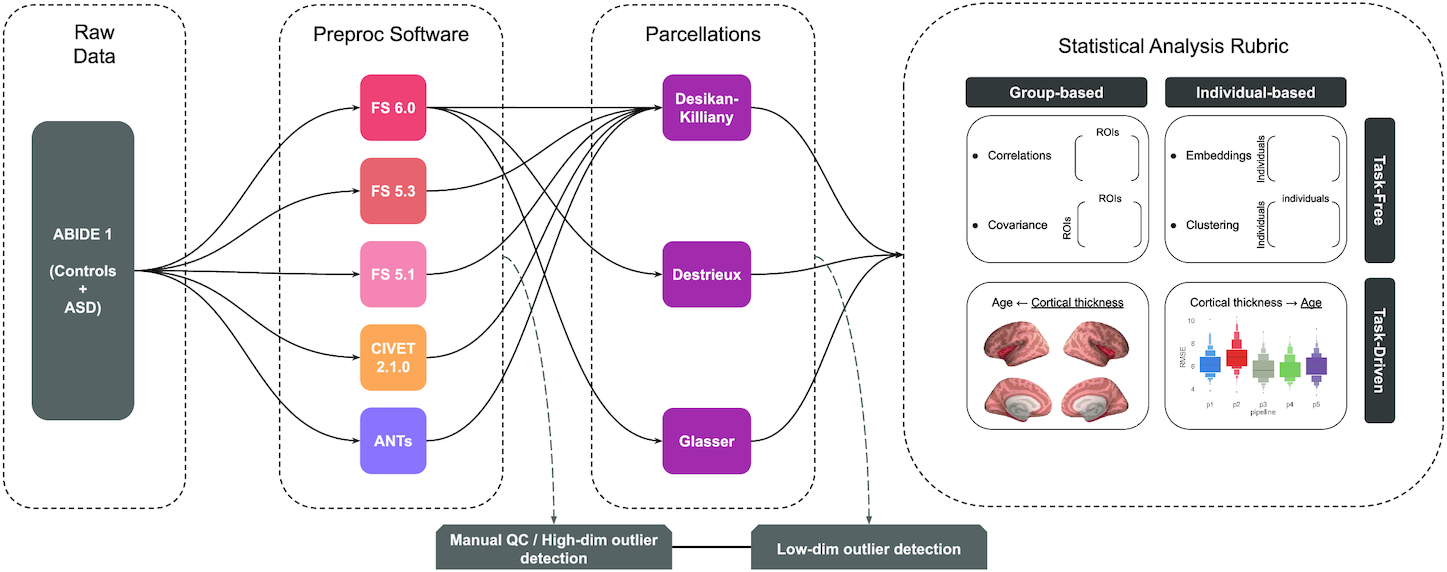
\includegraphics[width=10cm]{data/pipeline.jpeg}
			};
			\node[align=center, font=\scriptsize\linespread{1.1}\selectfont] at ($ (image.south) - (0, 0.7) $) {
				"Understanding the impact of preprocessing pipelines on neuroimaging cortical surface analyses.", \\
				Bhagwat et al. 2021, \textit{GigaScience}, \href{https://doi.org/10.1093/gigascience/giaa155}{https://doi.org/10.1093/gigascience/giaa155}
			};
		\end{tikzpicture}
		\vfill
	\end{frame}

	\begin{frame}{Introduction} % Group differences
		\centering
		\vfill
		\begin{tikzpicture}
			\node[inner sep=4pt, draw=black, fill=white] (image) {
				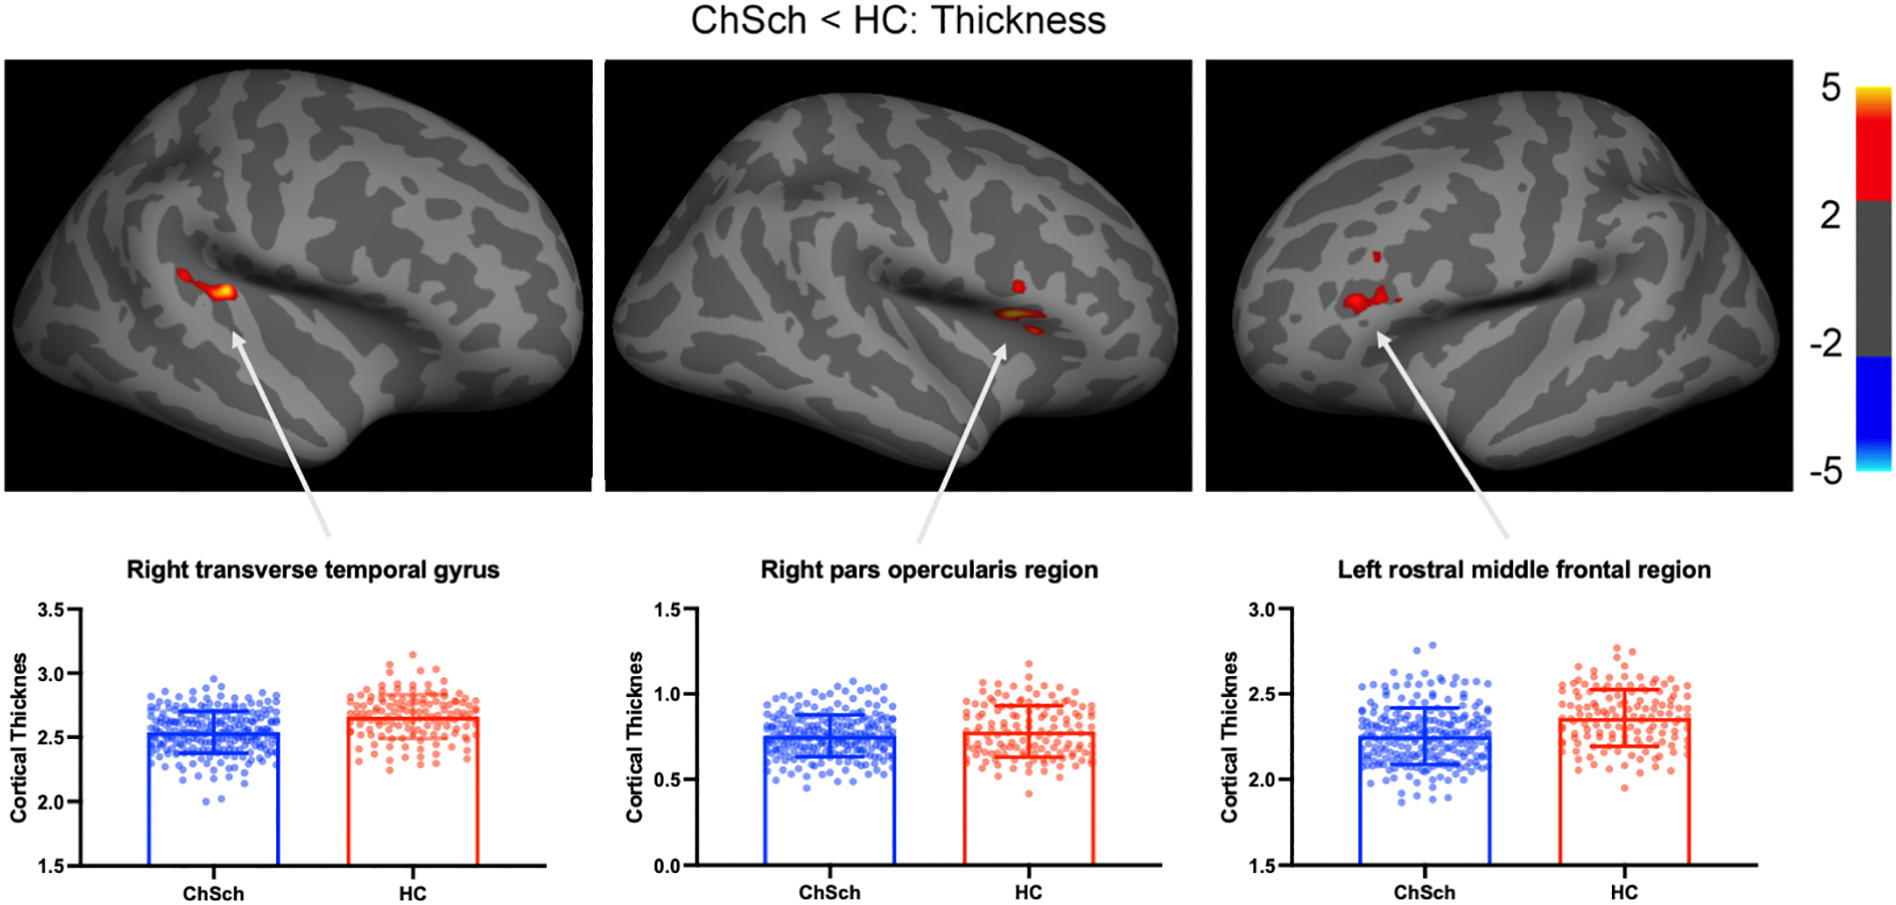
\includegraphics[width=10cm]{data/traditional.jpg}
			};
			\node[align=center, font=\scriptsize\linespread{1.1}\selectfont] at ($ (image.south) - (0, 0.7) $) {
				"Cortical surface abnormalities are different depending on the stage of schizophrenia: A cross-sectional \\
				vertexwise mega-analysis of thickness, area and gyrification.",\\ Rosa et al. 2021, \textit{Schizophrenia Research}, \href{https://doi.org/10.1016/j.schres.2021.08.011}{https://doi.org/10.1016/j.schres.2021.08.011}
			};
		\end{tikzpicture}
		\vfill
	\end{frame}

	\begin{frame}{Introduction} % Little predictive value
		\centering
		\vfill
		\begin{tikzpicture}
			\node[inner sep=4pt, draw=black, fill=white] (image) {
				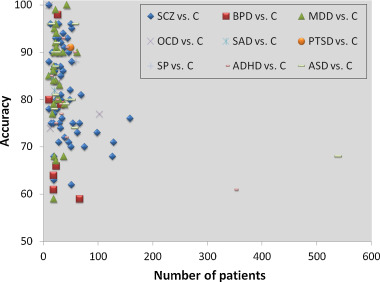
\includegraphics[width=5cm]{data/wolfers.jpg}
			};
			\node[align=center, font=\scriptsize\linespread{1.1}\selectfont] at ($ (image.south) - (0, 0.7) $) {
				"From estimating activation locality to predicting\\
				disorder: A review of pattern recognition for\\
				neuroimaging-based psychiatric diagnostics.",\\
				Wolfers et al. 2015, \textit{Neuroscience \& Biobehavioral Reviews},\\
				\href{https://doi.org/10.1016/j.neubiorev.2015.08.001}{https://doi.org/10.1016/j.neubiorev.2015.08.001}
			};
		\end{tikzpicture}
		\vfill
	\end{frame}

	\begin{frame}{Introduction} % Assumptions
		\centering
		\vfill
		\begin{tikzpicture}
			\node[inner sep=4pt, draw=black, fill=white] (image) {
				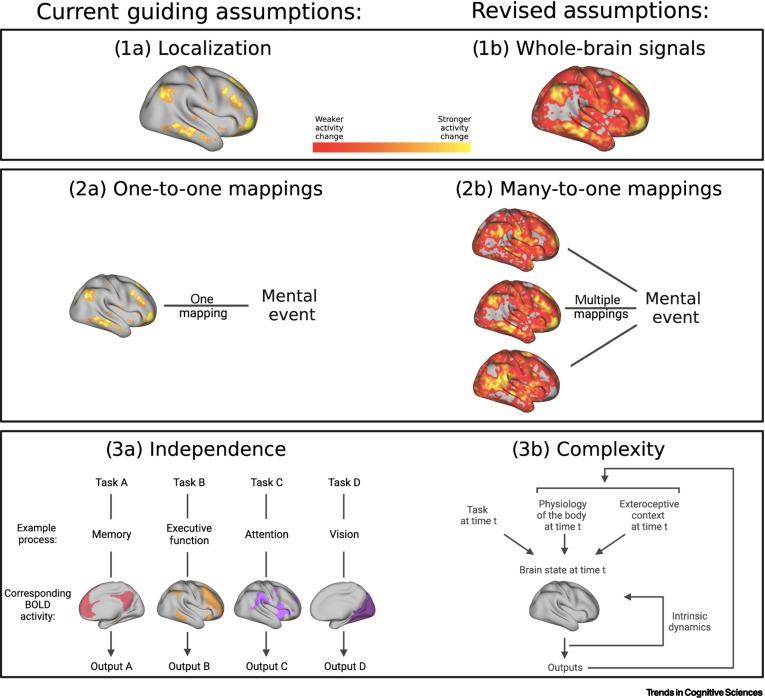
\includegraphics[width=6cm]{data/westlin.jpeg}
			};
			\node[align=center, font=\scriptsize\linespread{1.1}\selectfont] at ($ (image.south) - (0, 0.7) $) {
				"Improving the study of brain-behavior relationships by revisiting\\
				basic assumptions.",\\
				Westlin et al. 2023, \textit{Trends in Cognitive Sciences},\\
				\href{https://doi.org/10.1016/j.tics.2022.12.015}{https://doi.org/10.1016/j.tics.2022.12.015}
			};
		\end{tikzpicture}
		\vfill
	\end{frame}

	\begin{frame}{Introduction} % Simulated data
		\centering
		\vfill

		\begin{tikzpicture}
			\begin{axis}[
				xlabel=\small{Left hippocampus volume},
				ylabel=\small{Right hippocampus volume},
				xtick=\empty,
				ytick=\empty,
				height=7cm,
				width=7cm,
				xmin=-3,
				xmax=15,
				ymin=-4,
				ymax=13,
				clip=false
			]
				\addplot[
					only marks,
					mark=*,
					draw=blue,
					opacity=0.5,
					fill=blue!50
				] table [
					col sep=comma,
					x=control_x,
					y=control_y
				] {data/case_control_points.csv};
				\addplot[
					only marks,
					mark=*,
					draw=red,
					opacity=0.5,
					fill=red!50
				] table [
					col sep=comma,
					x=case_x,
					y=case_y
				] {data/case_control_points.csv};

				\node[
					draw=red,
					fill=red!50,
					circle,
					opacity=0.5,
					inner sep=1.4pt
				] (cases-legend) at (axis cs: 10.3, -3) {};
				\node[anchor=west, text depth=0] at ($ (cases-legend.east) + (-1, 0) $) {\small{Patients}};
				\node[
					draw=blue,
					fill=blue!50,
					circle,
					opacity=0.5,
					inner sep=1.4pt
				] (control-legend) at ($ (cases-legend.north) + (0, 6) $) {};
				\node[anchor=west, text depth=0] at ($ (control-legend.east) + (-1, 0) $) {\small{Controls}};
				\node[] at (axis cs: -5, -5) {};
				\node[] at (axis cs: 19.6, 17.3) {};
			\end{axis}
		\end{tikzpicture}
		\vfill
	\end{frame}

	\begin{frame}{Introduction} % Decision line
		\centering
		\vfill

		\begin{tikzpicture}
			\begin{axis}[
				xlabel=\small{Left hippocampus volume},
				ylabel=\small{Right hippocampus volume},
				xtick=\empty,
				ytick=\empty,
				height=7cm,
				width=7cm,
				xmin=-3,
				xmax=15,
				ymin=-4,
				ymax=13,
				clip=false
			]
				\addplot[
					only marks,
					mark=*,
					draw=blue,
					opacity=0.5,
					fill=blue!50
				] table [
					col sep=comma,
					x=control_x,
					y=control_y
				] {data/case_control_points.csv};
				\addplot[
					only marks,
					mark=*,
					draw=red,
					opacity=0.5,
					fill=red!50
				] table [
					col sep=comma,
					x=case_x,
					y=case_y
				] {data/case_control_points.csv};
				\addplot[dashed] coordinates {
					(-1.7, -3)
					(12.9, 11.6)
				};
				\node[
					draw=red,
					fill=red!50,
					circle,
					opacity=0.5,
					inner sep=1.4pt
				] (cases-legend) at (axis cs: 10.3, -3) {};
				\node[anchor=west, text depth=0] at ($ (cases-legend.east) + (-1, 0) $) {\small{Patients}};
				\node[
					draw=blue,
					fill=blue!50,
					circle,
					opacity=0.5,
					inner sep=1.4pt
				] (control-legend) at ($ (cases-legend.north) + (0, 6) $) {};
				\node[anchor=west, text depth=0] at ($ (control-legend.east) + (-1, 0) $) {\small{Controls}};
				\node[] at (axis cs: -5, -5) {};
				\node[] at (axis cs: 19.6, 17.3) {};
			\end{axis}
		\end{tikzpicture}
		\vfill
	\end{frame}

	\begin{frame}{Introduction} % Group differences
		\newsavebox{\xbox}
		\sbox{\xbox}{%
			\begin{tikzpicture}
				\begin{axis}[
					xmin=-3,
					xmax=16,
					ymin=0,
					ymax=1,
					width=7cm,
					height=3cm,
					axis line style={draw=none},
					tick style={draw=none},
					x dir=reverse,
					xtick=\empty,
					ytick=\empty
				]
					\addplot[draw=none, name path=zero] coordinates {
						(-5.80, 0)
						(17.38, 0)
					};
					\addplot[name path=case,draw=none] table [
						col sep=comma,
						x=x,
						y=case
					] {data/case_control_x_distributions.csv};
					\tikzfillbetween[of=zero and case]{blue, opacity=0.2};
					\addplot[name path=control,draw=none] table [
						col sep=comma,
						x=x,
						y=control
					] {data/case_control_x_distributions.csv};
					\tikzfillbetween[of=zero and control]{red, opacity=0.2};
				\end{axis}
			\end{tikzpicture}
		}


		\newsavebox{\ybox}
		\sbox{\ybox}{%
			\begin{tikzpicture}
				\begin{axis}[
					xmin=-5,
					xmax=15,
					ymin=0,
					ymax=1,
					width=7cm,
					height=3cm,
					axis line style={draw=none},
					tick style={draw=none},
					xtick=\empty,
					ytick=\empty
				]
					\addplot[draw=none, name path=zero] coordinates {
						(-5.80, 0)
						(17.38, 0)
					};
					\addplot[name path=case,draw=none] table [
						col sep=comma,
						x=y,
						y=case
					] {data/case_control_y_distributions.csv};
					\tikzfillbetween[of=zero and case]{blue, opacity=0.2};
					\addplot[name path=control,draw=none] table [
						col sep=comma,
						x=y,
						y=control
					] {data/case_control_y_distributions.csv};
					\tikzfillbetween[of=zero and control]{red, opacity=0.2};
				\end{axis}
			\end{tikzpicture}
		}

		\centering
		\vfill

		\begin{tikzpicture}
			\begin{axis}[
				xlabel=\small{Left hippocampus volume},
				ylabel=\small{Right hippocampus volume},
				xtick=\empty,
				ytick=\empty,
				height=7cm,
				width=7cm,
				xmin=-3,
				xmax=15,
				ymin=-4,
				ymax=13,
				clip=false
			]
				\addplot[
					only marks,
					mark=*,
					draw=blue,
					opacity=0.5,
					fill=blue!50
				] table [
					col sep=comma,
					x=control_x,
					y=control_y
				] {data/case_control_points.csv};
				\addplot[
					only marks,
					mark=*,
					draw=red,
					opacity=0.5,
					fill=red!50
				] table [
					col sep=comma,
					x=case_x,
					y=case_y
				] {data/case_control_points.csv};
				\addplot[dashed] coordinates {
					(-1.7, -3)
					(12.9, 11.6)
				};
				\node[anchor=south,rotate=270, inner sep=0pt, outer sep=0pt] at (axis cs: 15, 4.454) {\usebox{\xbox}};
				\node[anchor=south, inner sep=0pt, outer sep=0pt] at (axis cs: 6.15, 13) {\usebox{\ybox}};
				\node[
					draw=red,
					fill=red!50,
					circle,
					opacity=0.5,
					inner sep=1.4pt
				] (cases-legend) at (axis cs: 10.3, -3) {};
				\node[anchor=west, text depth=0] at ($ (cases-legend.east) + (-1, 0) $) {\small{Patients}};
				\node[
					draw=blue,
					fill=blue!50,
					circle,
					opacity=0.5,
					inner sep=1.4pt
				] (control-legend) at ($ (cases-legend.north) + (0, 6) $) {};
				\node[anchor=west, text depth=0] at ($ (control-legend.east) + (-1, 0) $) {\small{Controls}};
				\node[] at (axis cs: -5, -5) {};
				\node[] at (axis cs: 19.6, 17.3) {};
			\end{axis}
		\end{tikzpicture}
		\vfill
	\end{frame}

	\begin{frame}{Introduction} % GLM
		\centering
		\vfill
		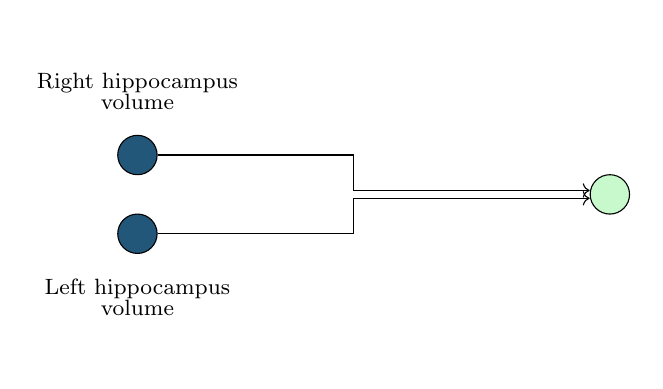
\begin{tikzpicture}
			\node[
				draw=black,
				fill=input,
				circle,
				minimum size=0.5cm,
				label={[align=center, font=\footnotesize\linespread{0.8}\selectfont, label distance=0.2cm]above:{Right hippocampus\\volume}}
			] (in1)at (0, 0) {};
			\node[
				draw=black,
				fill=input,
				circle,
				minimum size=0.5cm,
				label={[align=center, font=\footnotesize\linespread{0.8}\selectfont, label distance=0.2cm]below:{Left hippocampus\\volume}}
			] (in2) at (0, -1) {};

			\node[
				draw=black,
				minimum size=0.5cm,
				circle,
				fill=output
			] (out) at (6, -0.5) {};

			\draw[->] (in1) -| ($ (out.west) - (3, -0.05) $) -- ($ (out.west) + (0, 0.05) $);
			\draw[->] (in2) -| ($ (out.west) - (3, 0.05) $) -- ($ (out.west) + (0, -0.05) $);

			\node[] at (-0.9, -2.5) {};
			\node[] at (6.2, 1.5) {};
		\end{tikzpicture}
		\vfill
	\end{frame}

	\begin{frame}{Introduction} % Interaction
		\centering
		\vfill
		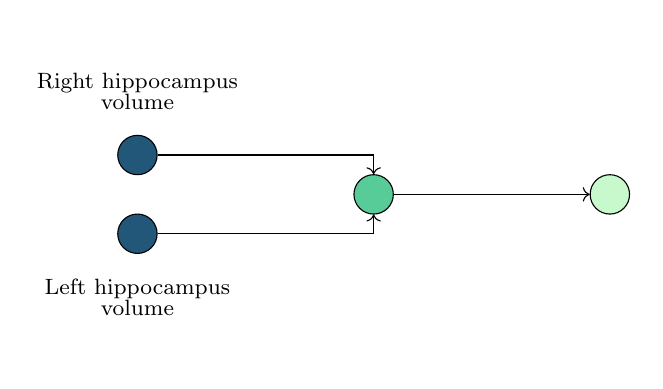
\begin{tikzpicture}
			\node[
				draw=black,
				fill=input,
				circle,
				minimum size=0.5cm,
				label={[align=center, font=\footnotesize\linespread{0.8}\selectfont, label distance=0.2cm]above:{Right hippocampus\\volume}}
			] (in1)at (0, 0) {};
			\node[
				draw=black,
				fill=input,
				circle,
				minimum size=0.5cm,
				label={[align=center, font=\footnotesize\linespread{0.8}\selectfont, label distance=0.2cm]below:{Left hippocampus\\volume}}
			] (in2) at (0, -1) {};


			\node[
				draw=black,
				minimum size=0.5cm,
				circle,
				fill=second
			] (n10) at (3, -0.5) {};

			\node[
				draw=black,
				minimum size=0.5cm,
				circle,
				fill=output
			] (out) at (6, -0.5) {};

			\draw[->] (in1) -| (n10.north);
			\draw[->] (in2) -| (n10.south);
			\draw[->] (n10) -- (out);

			\node[] at (-0.9, -2.5) {};
			\node[] at (6.2, 1.5) {};
		\end{tikzpicture}
		\vfill
	\end{frame}

	\begin{frame}{Introduction} % Neural network
		\centering
		\vfill
		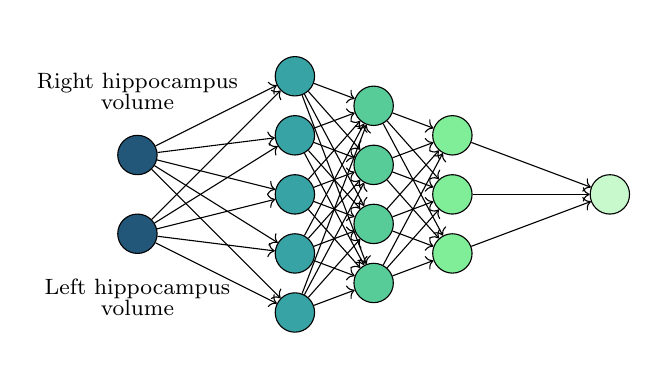
\begin{tikzpicture}
			\node[
				draw=black,
				fill=input,
				circle,
				minimum size=0.5cm,
				label={[align=center, font=\footnotesize\linespread{0.8}\selectfont, label distance=0.2cm]above:{Right hippocampus\\volume}}
			] (in1)at (0, 0) {};
			\node[
				draw=black,
				fill=input,
				circle,
				minimum size=0.5cm,
				label={[align=center, font=\footnotesize\linespread{0.8}\selectfont, label distance=0.2cm]below:{Left hippocampus\\volume}}
			] (in2) at (0, -1) {};

			\node[
				draw=black,
				minimum size=0.5cm,
				circle,
				fill=first
			] (n00) at (2, 1) {};
			\node[
				draw=black,
				minimum size=0.5cm,
				circle,
				fill=first
			] (n01) at (2, 0.25) {};
			\node[
				draw=black,
				minimum size=0.5cm,
				circle,
				fill=first
			] (n02) at (2, -0.5) {};
			\node[
				draw=black,
				minimum size=0.5cm,
				circle,
				fill=first
			] (n03) at (2, -1.25) {};
			\node[
				draw=black,
				minimum size=0.5cm,
				circle,
				fill=first
			] (n04) at (2, -2) {};

			\node[
				draw=black,
				minimum size=0.5cm,
				circle,
				fill=second
			] (n10) at (3, 0.625) {};
			\node[
				draw=black,
				minimum size=0.5cm,
				circle,
				fill=second
			] (n11) at (3, -0.125) {};
			\node[
				draw=black,
				minimum size=0.5cm,
				circle,
				fill=second
			] (n12) at (3, -0.875) {};
			\node[
				draw=black,
				minimum size=0.5cm,
				circle,
				fill=second
			] (n13) at (3, -1.625) {};

			\node[
				draw=black,
				minimum size=0.5cm,
				circle,
				fill=third
			] (n20) at (4, 0.25) {};
			\node[
				draw=black,
				minimum size=0.5cm,
				circle,
				fill=third
			] (n21) at (4, -0.5) {};
			\node[
				draw=black,
				minimum size=0.5cm,
				circle,
				fill=third
			] (n22) at (4, -1.25) {};

			\node[
				draw=black,
				minimum size=0.5cm,
				circle,
				fill=output
			] (out) at (6, -0.5) {};

			\draw[->] (in1) -- (n00);
			\draw[->] (in1) -- (n01);
			\draw[->] (in1) -- (n02);
			\draw[->] (in1) -- (n03);
			\draw[->] (in1) -- (n04);

			\draw[->] (in2) -- (n00);
			\draw[->] (in2) -- (n01);
			\draw[->] (in2) -- (n02);
			\draw[->] (in2) -- (n03);
			\draw[->] (in2) -- (n04);

			\draw[->] (n00) -- (n10);
			\draw[->] (n00) -- (n11);
			\draw[->] (n00) -- (n12);
			\draw[->] (n00) -- (n13);

			\draw[->] (n01) -- (n10);
			\draw[->] (n01) -- (n11);
			\draw[->] (n01) -- (n12);
			\draw[->] (n01) -- (n13);

			\draw[->] (n02) -- (n10);
			\draw[->] (n02) -- (n11);
			\draw[->] (n02) -- (n12);
			\draw[->] (n02) -- (n13);

			\draw[->] (n03) -- (n10);
			\draw[->] (n03) -- (n11);
			\draw[->] (n03) -- (n12);
			\draw[->] (n03) -- (n13);

			\draw[->] (n04) -- (n10);
			\draw[->] (n04) -- (n11);
			\draw[->] (n04) -- (n12);
			\draw[->] (n04) -- (n13);

			\draw[->] (n10) -- (n20);
			\draw[->] (n10) -- (n21);
			\draw[->] (n10) -- (n22);

			\draw[->] (n11) -- (n20);
			\draw[->] (n11) -- (n21);
			\draw[->] (n11) -- (n22);

			\draw[->] (n12) -- (n20);
			\draw[->] (n12) -- (n21);
			\draw[->] (n12) -- (n22);

			\draw[->] (n13) -- (n20);
			\draw[->] (n13) -- (n21);
			\draw[->] (n13) -- (n22);

			\draw[->] (n20) -- (out);
			\draw[->] (n21) -- (out);
			\draw[->] (n22) -- (out);

			\node[] at (-0.9, -2.5) {};
			\node[] at (6.2, 1.5) {};
		\end{tikzpicture}
		\vfill
	\end{frame}

	\begin{frame}{Introduction} % Neural network
		\centering
		\vfill
		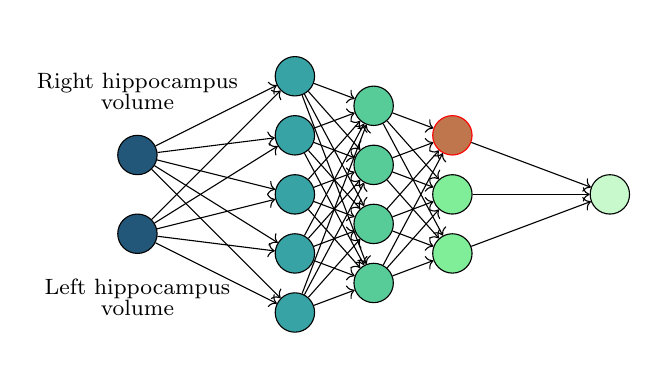
\begin{tikzpicture}
			\node[
				draw=black,
				fill=input,
				circle,
				minimum size=0.5cm,
				label={[align=center, font=\footnotesize\linespread{0.8}\selectfont, label distance=0.2cm]above:{Right hippocampus\\volume}}
			] (in1)at (0, 0) {};
			\node[
				draw=black,
				fill=input,
				circle,
				minimum size=0.5cm,
				label={[align=center, font=\footnotesize\linespread{0.8}\selectfont, label distance=0.2cm]below:{Left hippocampus\\volume}}
			] (in2) at (0, -1) {};

			\node[
				draw=black,
				minimum size=0.5cm,
				circle,
				fill=first
			] (n00) at (2, 1) {};
			\node[
				draw=black,
				minimum size=0.5cm,
				circle,
				fill=first
			] (n01) at (2, 0.25) {};
			\node[
				draw=black,
				minimum size=0.5cm,
				circle,
				fill=first
			] (n02) at (2, -0.5) {};
			\node[
				draw=black,
				minimum size=0.5cm,
				circle,
				fill=first
			] (n03) at (2, -1.25) {};
			\node[
				draw=black,
				minimum size=0.5cm,
				circle,
				fill=first
			] (n04) at (2, -2) {};

			\node[
				draw=black,
				minimum size=0.5cm,
				circle,
				fill=second
			] (n10) at (3, 0.625) {};
			\node[
				draw=black,
				minimum size=0.5cm,
				circle,
				fill=second
			] (n11) at (3, -0.125) {};
			\node[
				draw=black,
				minimum size=0.5cm,
				circle,
				fill=second
			] (n12) at (3, -0.875) {};
			\node[
				draw=black,
				minimum size=0.5cm,
				circle,
				fill=second
			] (n13) at (3, -1.625) {};

			\node[
				draw=red,
				minimum size=0.5cm,
				circle,
				fill=third!50!red
			] (n20) at (4, 0.25) {};
			\node[
				draw=black,
				minimum size=0.5cm,
				circle,
				fill=third
			] (n21) at (4, -0.5) {};
			\node[
				draw=black,
				minimum size=0.5cm,
				circle,
				fill=third
			] (n22) at (4, -1.25) {};

			\node[
				draw=black,
				minimum size=0.5cm,
				circle,
				fill=output
			] (out) at (6, -0.5) {};

			\draw[->] (in1) -- (n00);
			\draw[->] (in1) -- (n01);
			\draw[->] (in1) -- (n02);
			\draw[->] (in1) -- (n03);
			\draw[->] (in1) -- (n04);

			\draw[->] (in2) -- (n00);
			\draw[->] (in2) -- (n01);
			\draw[->] (in2) -- (n02);
			\draw[->] (in2) -- (n03);
			\draw[->] (in2) -- (n04);

			\draw[->] (n00) -- (n10);
			\draw[->] (n00) -- (n11);
			\draw[->] (n00) -- (n12);
			\draw[->] (n00) -- (n13);

			\draw[->] (n01) -- (n10);
			\draw[->] (n01) -- (n11);
			\draw[->] (n01) -- (n12);
			\draw[->] (n01) -- (n13);

			\draw[->] (n02) -- (n10);
			\draw[->] (n02) -- (n11);
			\draw[->] (n02) -- (n12);
			\draw[->] (n02) -- (n13);

			\draw[->] (n03) -- (n10);
			\draw[->] (n03) -- (n11);
			\draw[->] (n03) -- (n12);
			\draw[->] (n03) -- (n13);

			\draw[->] (n04) -- (n10);
			\draw[->] (n04) -- (n11);
			\draw[->] (n04) -- (n12);
			\draw[->] (n04) -- (n13);

			\draw[->] (n10) -- (n20);
			\draw[->] (n10) -- (n21);
			\draw[->] (n10) -- (n22);

			\draw[->] (n11) -- (n20);
			\draw[->] (n11) -- (n21);
			\draw[->] (n11) -- (n22);

			\draw[->] (n12) -- (n20);
			\draw[->] (n12) -- (n21);
			\draw[->] (n12) -- (n22);

			\draw[->] (n13) -- (n20);
			\draw[->] (n13) -- (n21);
			\draw[->] (n13) -- (n22);

			\draw[->] (n20) -- (out);
			\draw[->] (n21) -- (out);
			\draw[->] (n22) -- (out);

			\node[] at (-0.9, -2.5) {};
			\node[] at (6.2, 1.5) {};
		\end{tikzpicture}
		\vfill
	\end{frame}

	\begin{frame}{Introduction} % Neural network
		\centering
		\vfill
		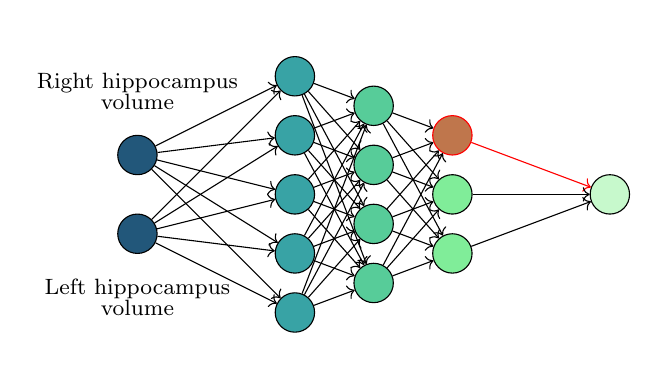
\begin{tikzpicture}
			\node[
				draw=black,
				fill=input,
				circle,
				minimum size=0.5cm,
				label={[align=center, font=\footnotesize\linespread{0.8}\selectfont, label distance=0.2cm]above:{Right hippocampus\\volume}}
			] (in1)at (0, 0) {};
			\node[
				draw=black,
				fill=input,
				circle,
				minimum size=0.5cm,
				label={[align=center, font=\footnotesize\linespread{0.8}\selectfont, label distance=0.2cm]below:{Left hippocampus\\volume}}
			] (in2) at (0, -1) {};

			\node[
				draw=black,
				minimum size=0.5cm,
				circle,
				fill=first
			] (n00) at (2, 1) {};
			\node[
				draw=black,
				minimum size=0.5cm,
				circle,
				fill=first
			] (n01) at (2, 0.25) {};
			\node[
				draw=black,
				minimum size=0.5cm,
				circle,
				fill=first
			] (n02) at (2, -0.5) {};
			\node[
				draw=black,
				minimum size=0.5cm,
				circle,
				fill=first
			] (n03) at (2, -1.25) {};
			\node[
				draw=black,
				minimum size=0.5cm,
				circle,
				fill=first
			] (n04) at (2, -2) {};

			\node[
				draw=black,
				minimum size=0.5cm,
				circle,
				fill=second
			] (n10) at (3, 0.625) {};
			\node[
				draw=black,
				minimum size=0.5cm,
				circle,
				fill=second
			] (n11) at (3, -0.125) {};
			\node[
				draw=black,
				minimum size=0.5cm,
				circle,
				fill=second
			] (n12) at (3, -0.875) {};
			\node[
				draw=black,
				minimum size=0.5cm,
				circle,
				fill=second
			] (n13) at (3, -1.625) {};

			\node[
				draw=red,
				minimum size=0.5cm,
				circle,
				fill=third!50!red
			] (n20) at (4, 0.25) {};
			\node[
				draw=black,
				minimum size=0.5cm,
				circle,
				fill=third
			] (n21) at (4, -0.5) {};
			\node[
				draw=black,
				minimum size=0.5cm,
				circle,
				fill=third
			] (n22) at (4, -1.25) {};

			\node[
				draw=black,
				minimum size=0.5cm,
				circle,
				fill=output
			] (out) at (6, -0.5) {};

			\draw[->] (in1) -- (n00);
			\draw[->] (in1) -- (n01);
			\draw[->] (in1) -- (n02);
			\draw[->] (in1) -- (n03);
			\draw[->] (in1) -- (n04);

			\draw[->] (in2) -- (n00);
			\draw[->] (in2) -- (n01);
			\draw[->] (in2) -- (n02);
			\draw[->] (in2) -- (n03);
			\draw[->] (in2) -- (n04);

			\draw[->] (n00) -- (n10);
			\draw[->] (n00) -- (n11);
			\draw[->] (n00) -- (n12);
			\draw[->] (n00) -- (n13);

			\draw[->] (n01) -- (n10);
			\draw[->] (n01) -- (n11);
			\draw[->] (n01) -- (n12);
			\draw[->] (n01) -- (n13);

			\draw[->] (n02) -- (n10);
			\draw[->] (n02) -- (n11);
			\draw[->] (n02) -- (n12);
			\draw[->] (n02) -- (n13);

			\draw[->] (n03) -- (n10);
			\draw[->] (n03) -- (n11);
			\draw[->] (n03) -- (n12);
			\draw[->] (n03) -- (n13);

			\draw[->] (n04) -- (n10);
			\draw[->] (n04) -- (n11);
			\draw[->] (n04) -- (n12);
			\draw[->] (n04) -- (n13);

			\draw[->] (n10) -- (n20);
			\draw[->] (n10) -- (n21);
			\draw[->] (n10) -- (n22);

			\draw[->] (n11) -- (n20);
			\draw[->] (n11) -- (n21);
			\draw[->] (n11) -- (n22);

			\draw[->] (n12) -- (n20);
			\draw[->] (n12) -- (n21);
			\draw[->] (n12) -- (n22);

			\draw[->] (n13) -- (n20);
			\draw[->] (n13) -- (n21);
			\draw[->] (n13) -- (n22);

			\draw[red,->] (n20) -- (out);
			\draw[->] (n21) -- (out);
			\draw[->] (n22) -- (out);

			\node[] at (-0.9, -2.5) {};
			\node[] at (6.2, 1.5) {};
		\end{tikzpicture}
		\vfill
	\end{frame}

	\begin{frame}{Introduction} % Black box
		\centering
		\vfill
		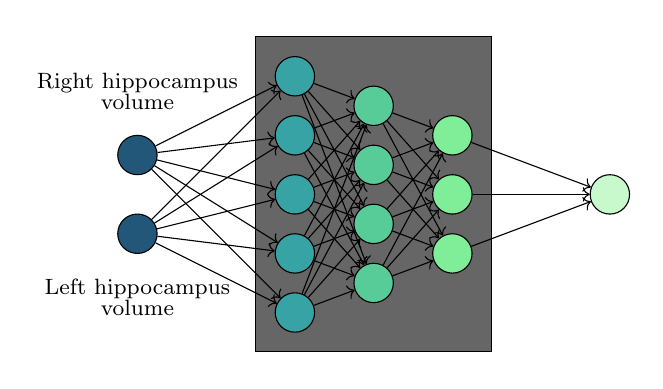
\begin{tikzpicture}
			% Box which emcopasses the nodes in the three middle layers
			\draw[draw=black, fill=black!60] (1.5, -2.5) rectangle (4.5, 1.5);
			\node[
				draw=black,
				fill=input,
				circle,
				minimum size=0.5cm,
				label={[align=center, font=\footnotesize\linespread{0.8}\selectfont, label distance=0.2cm]above:{Right hippocampus\\volume}}
			] (in1)at (0, 0) {};
			\node[
				draw=black,
				fill=input,
				circle,
				minimum size=0.5cm,
				label={[align=center, font=\footnotesize\linespread{0.8}\selectfont, label distance=0.2cm]below:{Left hippocampus\\volume}}
			] (in2) at (0, -1) {};

			\node[
				draw=black,
				minimum size=0.5cm,
				circle,
				fill=first
			] (n00) at (2, 1) {};
			\node[
				draw=black,
				minimum size=0.5cm,
				circle,
				fill=first
			] (n01) at (2, 0.25) {};
			\node[
				draw=black,
				minimum size=0.5cm,
				circle,
				fill=first
			] (n02) at (2, -0.5) {};
			\node[
				draw=black,
				minimum size=0.5cm,
				circle,
				fill=first
			] (n03) at (2, -1.25) {};
			\node[
				draw=black,
				minimum size=0.5cm,
				circle,
				fill=first
			] (n04) at (2, -2) {};

			\node[
				draw=black,
				minimum size=0.5cm,
				circle,
				fill=second
			] (n10) at (3, 0.625) {};
			\node[
				draw=black,
				minimum size=0.5cm,
				circle,
				fill=second
			] (n11) at (3, -0.125) {};
			\node[
				draw=black,
				minimum size=0.5cm,
				circle,
				fill=second
			] (n12) at (3, -0.875) {};
			\node[
				draw=black,
				minimum size=0.5cm,
				circle,
				fill=second
			] (n13) at (3, -1.625) {};

			\node[
				draw=black,
				minimum size=0.5cm,
				circle,
				fill=third
			] (n20) at (4, 0.25) {};
			\node[
				draw=black,
				minimum size=0.5cm,
				circle,
				fill=third
			] (n21) at (4, -0.5) {};
			\node[
				draw=black,
				minimum size=0.5cm,
				circle,
				fill=third
			] (n22) at (4, -1.25) {};

			\node[
				draw=black,
				minimum size=0.5cm,
				circle,
				fill=output
			] (out) at (6, -0.5) {};

			\draw[->] (in1) -- (n00);
			\draw[->] (in1) -- (n01);
			\draw[->] (in1) -- (n02);
			\draw[->] (in1) -- (n03);
			\draw[->] (in1) -- (n04);

			\draw[->] (in2) -- (n00);
			\draw[->] (in2) -- (n01);
			\draw[->] (in2) -- (n02);
			\draw[->] (in2) -- (n03);
			\draw[->] (in2) -- (n04);

			\draw[->] (n00) -- (n10);
			\draw[->] (n00) -- (n11);
			\draw[->] (n00) -- (n12);
			\draw[->] (n00) -- (n13);

			\draw[->] (n01) -- (n10);
			\draw[->] (n01) -- (n11);
			\draw[->] (n01) -- (n12);
			\draw[->] (n01) -- (n13);

			\draw[->] (n02) -- (n10);
			\draw[->] (n02) -- (n11);
			\draw[->] (n02) -- (n12);
			\draw[->] (n02) -- (n13);

			\draw[->] (n03) -- (n10);
			\draw[->] (n03) -- (n11);
			\draw[->] (n03) -- (n12);
			\draw[->] (n03) -- (n13);

			\draw[->] (n04) -- (n10);
			\draw[->] (n04) -- (n11);
			\draw[->] (n04) -- (n12);
			\draw[->] (n04) -- (n13);

			\draw[->] (n10) -- (n20);
			\draw[->] (n10) -- (n21);
			\draw[->] (n10) -- (n22);

			\draw[->] (n11) -- (n20);
			\draw[->] (n11) -- (n21);
			\draw[->] (n11) -- (n22);

			\draw[->] (n12) -- (n20);
			\draw[->] (n12) -- (n21);
			\draw[->] (n12) -- (n22);

			\draw[->] (n13) -- (n20);
			\draw[->] (n13) -- (n21);
			\draw[->] (n13) -- (n22);

			\draw[->] (n20) -- (out);
			\draw[->] (n21) -- (out);
			\draw[->] (n22) -- (out);

			\node[] at (-0.9, -2.5) {};
			\node[] at (6.2, 1.5) {};
		\end{tikzpicture}
		\vfill
	\end{frame}

	\begin{frame}{Introduction}
		\begin{itemize}
			\item There are high level abstractions that could help delineate the relationship between the brain as represented in neuroimaging data and mental and neurological conditions.
			\item Deep neural networks epitomize the expressive capacity to learn and utilize these abstractions.
			\item Approaches need to allow for interpretations of the abstractions themselves.
		\end{itemize}
	\end{frame}

	\begin{frame}{Paper 1: Brain age} % Title
		\centering
		\vfill
		\begin{tikzpicture}
			\node[inner sep=1pt, fill=white, draw=black] {
				
\includegraphics[width=8cm]{data/paper1.png}
			};
		\end{tikzpicture}
		\vfill
	\end{frame}

	\begin{frame}{Paper 1: Brain age} % Dataset
		\centering
		\vfill
		\begin{tikzpicture}
			\begin{axis}[
				width=0.9\textwidth,
				height=0.65\textwidth,
				xmin=0,
				xmax=100,
				ymin=-1200,
				ymax=1200,
				yticklabels={,,},
				ytick=\empty,
				xtick pos=bottom,
				y dir=reverse,
				axis x line=middle,
				axis y line=none,
				xtick={0,10,20,30,40,50,60,70,80}
			]
				\addplot [draw=none, name path=zero] coordinates {
					(0, 0)
					(100, 0)
				};

				\addplot [draw=none, name path=hbn] table [col sep=comma, x=age,y=hbn] {data/paper1/dataset/M.csv};
				\addplot [hbn-clr] fill between [of=zero and hbn];
				\addplot [draw=none, name path=adhd200] table [col sep=comma, x=age,y=adhd200-hc] {data/paper1/dataset/M.csv};
				\addplot [adhd200-clr] fill between [of=hbn and adhd200];\label{trace:adhd200}
				\addplot [draw=none, name path=ping] table [col sep=comma, x=age,y=ping] {data/paper1/dataset/M.csv};
				\addplot [ping-clr] fill between [of=adhd200 and ping];\label{trace:ping}

				\addplot [draw=none, name path=ds000119] table [col sep=comma, x=age,y=ds000119] {data/paper1/dataset/M.csv};
				\addplot [ds000119-clr] fill between [of=ping and ds000119];\label{trace:ds000119}
				\addplot [draw=none, name path=abide] table [col sep=comma, x=age,y=abide-hc] {data/paper1/dataset/M.csv};
				\addplot [abide-clr] fill between [of=ds000119 and abide];\label{trace:abide}
				\addplot [draw=none, name path=slim] table [col sep=comma, x=age,y=slim] {data/paper1/dataset/M.csv};
				\addplot [slim-clr] fill between [of=abide and slim];\label{trace:slim}
				\addplot [draw=none, name path=abide2] table [col sep=comma, x=age,y=abide2-hc] {data/paper1/dataset/M.csv};
				\addplot [abide2-clr] fill between [of=slim and abide2];\label{trace:abide2}
				\addplot [draw=none, name path=beijing] table [col sep=comma, x=age,y=beijing-enhanced] {data/paper1/dataset/M.csv};
				\addplot [beijing-clr] fill between [of=slim and beijing];\label{trace:beijing}
				\addplot [draw=none, name path=aomic] table [col sep=comma, x=age,y=aomic-id1000] {data/paper1/dataset/M.csv};
				\addplot [aomic-clr] fill between [of=beijing and aomic];\label{trace:aomic}
				\addplot [draw=none, name path=corr] table [col sep=comma, x=age,y=corr] {data/paper1/dataset/M.csv};
				\addplot [corr-clr] fill between [of=aomic and corr];\label{trace:corr}
				\addplot [draw=none, name path=mpi] table [col sep=comma, x=age,y=mpi-lemon] {data/paper1/dataset/M.csv};
				\addplot [mpi-clr] fill between [of=corr and mpi];\label{trace:mpi}
				\addplot [draw=none, name path=hcp] table [col sep=comma, x=age,y=hcp] {data/paper1/dataset/M.csv};
				\addplot [hcp-clr] fill between [of=mpi and hcp];\label{trace:hcp}
				\addplot [draw=none, name path=fcon] table [col sep=comma, x=age,y=fcon1000] {data/paper1/dataset/M.csv};
				\addplot [fcon-clr] fill between [of=hcp and fcon];\label{trace:fcon}
				\addplot [draw=none, name path=nki] table [col sep=comma, x=age,y=nki-rockland] {data/paper1/dataset/M.csv};
				\addplot [nki-clr] fill between [of=fcon and nki];\label{trace:nki}
				\addplot [draw=none, name path=sald] table [col sep=comma, x=age,y=sald] {data/paper1/dataset/M.csv};
				\addplot [sald-clr] fill between [of=nki and sald];\label{trace:sald}
				\addplot [draw=none, name path=ds000222] table [col sep=comma, x=age,y=ds000222] {data/paper1/dataset/M.csv};
				\addplot [ds000222-clr] fill between [of=sald and ds000222];\label{trace:ds000222}
				\addplot [draw=none, name path=dlbs] table [col sep=comma, x=age,y=dlbs] {data/paper1/dataset/M.csv};
				\addplot [dlbs-clr] fill between [of=ds000222 and dlbs];\label{trace:dlbs}
				\addplot [draw=none, name path=camcan] table [col sep=comma, x=age,y=camcan] {data/paper1/dataset/M.csv};
				\addplot [camcan-clr] fill between [of=dlbs and camcan];\label{trace:camcan}
				\addplot [draw=none, name path=ukb] table [col sep=comma, x=age,y=ukb] {data/paper1/dataset/M.csv};
				\addplot [ukb-clr] fill between [of=camcan and ukb];\label{trace:ukb}
				\addplot [draw=black, name path=oasis] table [col sep=comma, x=age,y=oasis3-hc] {data/paper1/dataset/M.csv};
				\addplot [oasis-clr] fill between [of=ukb and oasis];\label{trace:oasis}

				\addplot [draw=none, name path=hbn] table [col sep=comma, x=age,y expr=\thisrow{hbn}*-1] {data/paper1/dataset/F.csv};
				\addplot [hbn-clr] fill between [of=zero and hbn];\label{trace:hbn}
				\addplot [draw=none, name path=adhd200] table [col sep=comma, x=age,y=,y expr=\thisrow{adhd200-hc}*-1] {data/paper1/dataset/F.csv};
				\addplot [adhd200-clr] fill between [of=hbn and adhd200];
				\addplot [draw=none, name path=ping] table [col sep=comma, x=age,y expr=\thisrow{ping}*-1] {data/paper1/dataset/F.csv};
				\addplot [ping-clr] fill between [of=adhd200 and ping];
				\addplot [draw=none, name path=abide] table [col sep=comma, x=age,y expr=\thisrow{abide-hc}*-1] {data/paper1/dataset/F.csv};
				\addplot [abide-clr] fill between [of=ping and abide];
				\addplot [draw=none, name path=abide2] table [col sep=comma, x=age,y expr=\thisrow{abide2-hc}*-1] {data/paper1/dataset/F.csv};
				\addplot [abide2-clr] fill between [of=abide and abide2];
				\addplot [draw=none, name path=ds000119] table [col sep=comma, x=age,y=,y expr=\thisrow{ds000119}*-1] {data/paper1/dataset/F.csv};
				\addplot [ds000119-clr] fill between [of=abide2 and ds000119];
				\addplot [draw=none, name path=slim] table [col sep=comma, x=age,y expr=\thisrow{slim}*-1] {data/paper1/dataset/F.csv};
				\addplot [slim-clr] fill between [of=ds000119 and slim];
				\addplot [draw=none, name path=beijing] table [col sep=comma, x=age,y expr=\thisrow{beijing-enhanced}*-1] {data/paper1/dataset/F.csv};
				\addplot [beijing-clr] fill between [of=slim and beijing];
				\addplot [draw=none, name path=ds000202] table [col sep=comma, x=age,y expr=\thisrow{ds000202}*-1] {data/paper1/dataset/F.csv};
				\addplot [ds000202-clr] fill between [of=beijing and ds000202];\label{trace:ds000202}
				\addplot [draw=none, name path=aomic] table [col sep=comma, x=age,y expr=\thisrow{aomic-id1000}*-1] {data/paper1/dataset/F.csv};
				\addplot [aomic-clr] fill between [of=beijing and aomic];
				\addplot [draw=none, name path=mpi] table [col sep=comma, x=age,y expr=\thisrow{mpi-lemon}*-1] {data/paper1/dataset/F.csv};
				\addplot [mpi-clr] fill between [of=aomic and mpi];
				\addplot [draw=none, name path=corr] table [col sep=comma, x=age,y expr=\thisrow{corr}*-1] {data/paper1/dataset/F.csv};
				\addplot [corr-clr] fill between [of=mpi and corr];
				\addplot [draw=none, name path=fcon] table [col sep=comma, x=age,y expr=\thisrow{fcon1000}*-1] {data/paper1/dataset/F.csv};
				\addplot [fcon-clr] fill between [of=corr and fcon];
				\addplot [draw=none, name path=hcp] table [col sep=comma, x=age, y expr=\thisrow{hcp}*-1] {data/paper1/dataset/F.csv};
				\addplot [hcp-clr] fill between [of=fcon and hcp];
				\addplot [draw=none, name path=nki] table [col sep=comma, x=age,y expr=\thisrow{nki-rockland}*-1] {data/paper1/dataset/F.csv};
				\addplot [nki-clr] fill between [of=hcp and nki];
				\addplot [draw=none, name path=ds000222] table [col sep=comma, x=age,y expr=\thisrow{ds000222}*-1] {data/paper1/dataset/F.csv};
				\addplot [ds000222-clr] fill between [of=nki and ds000222];
				\addplot [draw=none, name path=sald] table [col sep=comma, x=age,y expr=\thisrow{sald}*-1] {data/paper1/dataset/F.csv};
				\addplot [sald-clr] fill between [of=ds000222 and sald];
				\addplot [draw=none, name path=camcan] table [col sep=comma, x=age,y expr=\thisrow{camcan}*-1] {data/paper1/dataset/F.csv};
				\addplot [camcan-clr] fill between [of=sald and camcan];
				\addplot [draw=none, name path=dlbs] table [col sep=comma, x=age,y expr=\thisrow{dlbs}*-1] {data/paper1/dataset/F.csv};
				\addplot [dlbs-clr] fill between [of=camcan and dlbs];

				\addplot [draw=none, name path=ukb] table [col sep=comma, x=age,y expr=\thisrow{ukb}*-1] {data/paper1/dataset/F.csv};
				\addplot [ukb-clr] fill between [of=dlbs and ukb];
				\addplot [draw=black, name path=oasis] table [col sep=comma, x=age,y expr=\thisrow{oasis3-hc}*-1] {data/paper1/dataset/F.csv};
				\addplot [oasis-clr] fill between [of=ukb and oasis];

				\addplot [] coordinates {
					(0, 0)
					(100, 0)
				};
				\coordinate (male) at (axis cs:100,35) {};
				\coordinate (female) at (axis cs:100,-35) {};

				\node[] at (50,1056) {\textbf{\footnotesize{n=53542}}};
			\end{axis}
			\matrix [
				draw=none,
				matrix of nodes,
				anchor=north west,
				row sep=-0.1cm,
				font=\footnotesize,
				column 1/.style={anchor=base west}
			] at (8.2, 6.31) {
				\ref{trace:hbn} HBN \\
				\ref{trace:adhd200} ADHD200 \\
				\ref{trace:ping} PING \\
				\ref{trace:ds000119} ds000119 \\
				\ref{trace:abide} ABIDE \\
				\ref{trace:slim} SLIM \\
				\ref{trace:abide2} ABIDE2 \\
				\ref{trace:beijing} Beijing \\
				\ref{trace:aomic} AOMIC \\
				\ref{trace:corr} CoRR \\
				\ref{trace:mpi} MPI-Lemon \\
				\ref{trace:hcp} HCP \\
				\ref{trace:fcon} FCON1000 \\
				\ref{trace:nki} NKI Rockland \\
				\ref{trace:sald} SALD \\
				\ref{trace:ds000222} ds000222 \\
				\ref{trace:dlbs} DLBS \\
				\ref{trace:camcan} CamCAN \\
				\ref{trace:ukb} UKB \\
				\ref{trace:oasis} OASIS3 \\
				\ref{trace:ds000202} ds000202 \\
			};
			\node [anchor=north east] at (male) {\footnotesize{MALE}};
			\node [anchor=south east] at (female) {\footnotesize{FEMALE}};
		\end{tikzpicture}
		\vfill
	\end{frame}

	\begin{frame}{Paper 1: Brain age} % Model
		\begin{tikzpicture}
			\begin{axis}[
				axis line style={draw=none},
				xmin=-18.5,
				xmax=62,
				ymin=-8,
				ymax=12,
				width=1.125\textwidth,
				height=0.395\textwidth,
				ticks=none
			]

				\coordinate (start) at (axis cs: -4.75,3.9);
				\coordinate (input) at (axis cs: -1,3.9);

				\addplot[fill=conv-clr] coordinates {(0,0) (-1,0) (-1,6) (2,7.8) (3,7.8) (0,6) (0,0)};
				\addplot[fill=bn-clr] coordinates {(1,0) (0,0) (0,6) (3,7.8) (4,7.8) (1,6) (1,0)};
				\addplot[fill=relu-clr] coordinates {(2,0) (1,0) (1,6) (4,7.8) (5,7.8) (2,6) (2,0)};
				\addplot[fill=pool-clr] coordinates {(3,0) (2,0) (2,6) (5,7.8) (6,7.8) (3,6) (3,0)};
				\addplot[fill=pool-clr] coordinates {(3,0) (3,6) (6,7.8) (6,1.8) (3,0)};

				\draw [] (axis cs: 4.5,3.9) -- (axis cs: 8,3.9);

				\addplot[fill=conv-clr] coordinates {(8,0.65) (7,0.65) (7,5.65) (9.5,7.15) (10.5,7.15) (8,5.65) (8,0.65)};
				\addplot[fill=bn-clr] coordinates {(9,0.65) (8,0.65)  (8,5.65) (10.5,7.15) (11.5,7.15) (9,5.65) (9,0.65)};
				\addplot[fill=relu-clr] coordinates {(10,0.65) (9,0.65) (9,5.65) (11.5,7.15) (12.5,7.15) (10,5.65) (10,0.65)};
				\addplot[fill=pool-clr] coordinates {(11,0.65) (10,0.65) (10,5.65) (12.5,7.15) (13.5,7.15) (11,5.65) (11,0.65)};
				\addplot[fill=pool-clr] coordinates {(11,0.65) (11,5.65) (13.5,7.15) (13.5,2.15) (11,0.65)};

				\draw [] (axis cs: 12.25,3.9) -- (axis cs: 15.5,3.9);

				\addplot[fill=conv-clr] coordinates {(15.5,1.3) (14.5,1.3) (14.5,5.3) (16.5,6.5) (17.5,6.5) (15.5,5.3) (15.5,1.3)};
				\addplot[fill=bn-clr] coordinates {(16.5,1.3) (15.5,1.3) (15.5,5.3) (17.5,6.5) (18.5,6.5) (16.5,5.3) (16.5,1.3)};
				\addplot[fill=relu-clr] coordinates {(17.5,1.3) (16.5,1.3) (16.5,5.3) (18.5,6.5) (19.5,6.5) (17.5,5.3) (17.5,1.3)};
				\addplot[fill=pool-clr] coordinates {(18.5,1.3) (17.5,1.3) (17.5,5.3) (19.5,6.5) (20.5,6.5) (18.5,5.3) (18.5,1.3)};
				\addplot[fill=pool-clr] coordinates {(18.5,1.3) (18.5,5.3) (20.5,6.5) (20.5,2.5) (18.5,1.3)};

				\draw [] (axis cs: 19.5,3.9) -- (axis cs: 22.5,3.9);

				\addplot[fill=conv-clr] coordinates {(22.5,1.95) (21.5,1.95) (21.5,4.95) (23,5.85) (24,5.85) (22.5,4.95) (22.5,1.95)};
				\addplot[fill=bn-clr] coordinates {(23.5,1.95) (22.5,1.95) (22.5,4.95) (24,5.85) (25,5.85) (23.5,4.95) (23.5,1.95)};
				\addplot[fill=relu-clr] coordinates {(24.5,1.95) (23.5,1.95) (23.5,4.95) (25,5.85) (26,5.85) (24.5,4.95) (24.5,1.95)};
				\addplot[fill=pool-clr] coordinates {(25.5,1.95) (24.5,1.95) (24.5,4.95) (26,5.85) (27,5.85) (25.5,4.95) (25.5,1.95)};
				\addplot[fill=pool-clr] coordinates {(25.5,1.95) (25.5,4.95) (27,5.85) (27,2.85) (25.5,1.95)};

				\draw [] (axis cs: 26.25,3.9) -- (axis cs: 29,3.9);

				\addplot[fill=conv-clr] coordinates {(29,2.6) (28,2.6) (28,4.6) (29,5.2) (30,5.2) (29,4.6) (29,2.6)};
				\addplot[fill=bn-clr] coordinates {(30,2.6) (29,2.6) (29,4.6) (30,5.2) (31,5.2) (30,4.6) (30,2.6)};
				\addplot[fill=relu-clr] coordinates {(31,2.6) (30,2.6) (30,4.6) (31,5.2) (32,5.2) (31,4.6) (31,2.6)};
				\addplot[fill=pool-clr] coordinates {(32,2.6) (31,2.6) (31,4.6) (32,5.2) (33,5.2) (32,4.6) (32,2.6)};
				\addplot[fill=pool-clr] coordinates {(32,2.6) (32,4.6) (33,5.2) (33,3.2) (32,2.6)};

				\draw [] (axis cs: 32.5,3.9) -- (axis cs: 35,3.9);

				\addplot[fill=conv1x1-clr] coordinates {(35,3.25) (34,3.25) (34,4.25) (34.5,4.55) (35.5,4.55) (35,4.25) (35,3.25)};
				\addplot[fill=bn-clr] coordinates {(36,3.25) (35,3.25) (35,4.25) (35.5,4.55) (36.5,4.55) (36,4.25) (36,3.25)};
				\addplot[fill=relu-clr] coordinates {(37,3.25) (36,3.25) (36,4.25) (36.5,4.55) (37.5,4.55) (37,4.25) (37,3.25)};
				\addplot[fill=avgpool-clr] coordinates {(38,3.25) (37,3.25) (37,4.25) (37.5,4.55) (38.5,4.55) (38,4.25) (38,3.25)};
				\addplot[fill=dropout-clr] coordinates {(39,3.25) (38,3.25) (38,4.25) (38.5,4.55) (39.5,4.55) (39,4.25) (39,3.25)};
				\addplot[fill=dropout-clr] coordinates {(39,3.25) (39,4.25) (39.5,4.55) (39.5,3.55) (39,3.25)};

				\addplot[mark=square*,draw=black,fill=conv-clr,only marks] coordinates {(4,4)};\label{trace:conv}
				\addplot[mark=square*,draw=black,fill=bn-clr,only marks] coordinates {(4,4)};\label{trace:bn}
				\addplot[mark=square*,draw=black,fill=relu-clr,only marks] coordinates {(4,4)};\label{trace:relu}
				\addplot[mark=square*,draw=black,fill=pool-clr,only marks] coordinates {(4,4)};\label{trace:pool}
				\addplot[mark=square*,draw=black,fill=conv1x1-clr,only marks] coordinates {(4,4)};\label{trace:conv1}
				\addplot[mark=square*,draw=black,fill=avgpool-clr,only marks] coordinates {(4,4)};\label{trace:avgpool}
				\addplot[mark=square*,draw=black,fill=dropout-clr,only marks] coordinates {(4,4)};\label{trace:dropout}
				\addplot[mark=square*,draw=pool-clr,fill=pool-clr,only marks,mark size=0.1cm] coordinates {(4,4)};

				\coordinate (end) at (axis cs: 39.25,3.9);
				\node[draw=black,anchor=west,minimum height=0.3cm,minimum width=2.4cm,align=left, text depth=0] (regression) at (axis cs: 42.5,3.9) {\footnotesize{Regression}};
				\node[draw=black,anchor=west,minimum height=0.3cm,minimum width=2.4cm,align=right, text depth=0] (classification) at (axis cs: 42.5,6.9) {\footnotesize{Soft Classification}};
				\node[draw=black,anchor=west,minimum height=0.3cm,minimum width=2.4cm,align=left, text depth=0] (ranking) at (axis cs: 42.5,0.9) {\footnotesize{Ranking}};

				\draw[dashed] (axis cs: -2,8.8) -- (axis cs: 40.5,8.8) -- (axis cs: 40.5,-1) -- (axis cs: -2,-1) -- (axis cs: -2,8.8) ;
				\node [anchor=south] at (axis cs: 19.25,9.3) {\footnotesize{SFCN backbone}};

				\path [draw=black,->] (end) -- (regression.west) {};
				\path [draw=black,->] (end) -- (classification.west) {};
				\path [draw=black,->] (end) -- (ranking.west) {};

				\path [draw=black,-] (start) -- (input) {};

				\node [] at (axis cs: -9,4.5) {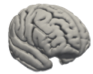
\includegraphics[scale=0.3]{data/brain.png}};

				\node [
					anchor=north,
					font=\footnotesize,
					align=center,
					draw=black
				] at (axis cs: 19.25,-2) {
					\ref{trace:conv} Conv3D (3,3,3) \ref{trace:conv1} Conv3D (1,1,1) \ref{trace:bn} BatchNorm \ref{trace:relu} ReLU \\ \ref{trace:pool} MaxPool3D (2,2,2) \ref{trace:avgpool} Global AvgPool3D \ref{trace:dropout} Dropout
				};

			\end{axis}
		\end{tikzpicture}
	\end{frame}

	\begin{frame}{Paper 1: Brain age} % Modelling approach
		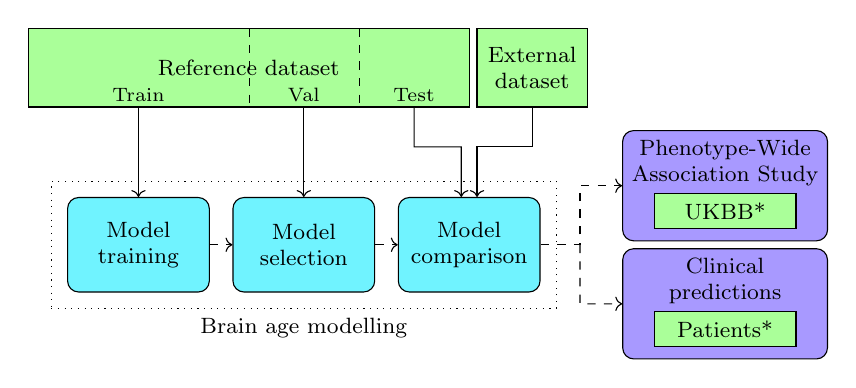
\begin{tikzpicture}[
			every node/.append style={font=\footnotesize}
		]
			\node[draw=black,minimum width=5.6cm,minimum height=1cm,fill=dataset] at (0.2,-1) {Reference dataset};
			\node[draw=none,minimum width=2.8cm,minimum height=1cm] (train) at (-1.2,-1.35) {\scriptsize{Train}};
			\node[draw=none,minimum width=1.4cm,minimum height=1cm] at (0.9,-1.35) (val) {\scriptsize{Val}};
			\node[draw=none,minimum width=1.4cm,minimum height=1cm] at (2.3,-1.35) (test) {\scriptsize{Test}};
			\node[draw=black,minimum height=1cm,minimum width=1.4cm,fill=dataset,align=center] (external) at (3.8,-1) {External\\dataset};
			\node[draw=black,rounded corners,align=center,minimum height=1.2cm, minimum width=1.8cm,fill=process] (training) at (-1.2,-3.25) {Model \\ training};
			\node[draw=black,rounded corners,align=center,minimum height=1.2cm, minimum width=1.8cm,fill=process] (selection) at (0.9,-3.25) {Model \\ selection};
			\node[draw=black,rounded corners,align=center,minimum height=1.2cm, minimum width=1.8cm,fill=process] (comparison) at (3,-3.25) {Model \\ comparison};
			\node[draw=black,rounded corners,align=center,minimum height=1.4cm, minimum width=2.6cm,fill=application, text depth=0.3cm] (pwas) at (6.25,-2.5) {Phenotype-Wide \\ Association Study \\};
			\node[draw=black,rounded corners,align=center,minimum height=1.4cm, minimum width=2.6cm,fill=application, text depth=0.3cm] (preds) at (6.25,-4) {Clinical \\ predictions \\};
			\node[draw=black,minimum height=0.4cm,minimum width=1.8cm,fill=dataset,align=center] at (6.25,-2.82) {UKBB*};
			\node[draw=black,minimum height=0.4cm,minimum width=1.8cm,fill=dataset,align=center] at (6.25,-4.32) {Patients*};
			\path[draw=black,->] ($ (train.south) + (0,0.35) $) -- (training) {};
			\path[draw=black,->] ($ (val.south) + (0,0.35) $) -- (selection) {};
			\path[draw=black,->] ($ (test.south) + (0,0.35) $) -- ($ (test.south) + (0,-0.15) $) -- ($ (test.south) + (0.6,-0.15) $) -- ($ (comparison.north) + (-0.1,0) $) {};
			\path[draw=black,->] (external.south) -- ($ (external.south) + (0,-0.5) $) -- ($ (external.south) + (-0.7,-0.5) $) -- ($ (comparison.north) + (0.1,0) $) {};
			\path[draw=black,->,dashed] (training) -- (selection) {};
			\path[draw=black,->,dashed] (selection) -- (comparison) {};
			\path[draw=black,->,dashed] (comparison.east) -- ($ (comparison.east) + (0.5,0) $) -- ($ (comparison.east) + (0.5,0.75) $) -- (pwas.west) {};
			\path[draw=black,->,dashed]($ (comparison.east) + (0.5,0) $) -- ($ (comparison.east) + (0.5,-0.75) $) -- (preds.west) {};
			\draw[dashed] ($ (train.east) + (0,0.85) $) -- ($ (train.east) + (0,-0.15) $) {};
			\draw[dashed] ($ (val.east) + (0,0.85) $) -- ($ (val.east) + (0,-0.15) $) {};

			\draw[dotted] ($ (training.south west) + (-0.2,-0.2) $) -- node[below] {Brain age modelling} ($ (comparison.south east) + (0.2,-0.2) $) -- ($ (comparison.north east) + (0.2,0.2) $) -- ($ (training.north west) + (-0.2,0.2) $) -- ($ (training.south west) + (-0.2,-0.2) $) {};
		\end{tikzpicture}
	\end{frame}

	\begin{frame}{Paper 1: Brain age} % Predictions
		\def\N{1}
		\centering
		\vfill
		\begin{tikzpicture}
			\begin{groupplot}[
				group style={
					group size=3 by 2,
					horizontal sep=0.4cm,
					vertical sep=0.8cm
				},
				width=0.4\linewidth,
				height=0.4\linewidth
			]

			  \nextgroupplot[
				  xmin=0,
				  xmax=100,
				  ymin=0,
				  ymax=100,
				  xtick pos=bottom,
				  ytick pos=left,
				  xticklabels={,,},
				  ticklabel style = {font=\footnotesize}
			  ]
				  \addplot [red] coordinates {(0,0) (100,100)};
				  \addplot [
					  only marks,
					  mark size=0.75pt,
					  color=black,
					  opacity=0.35
				  ] table [
					  x=classification,
					  y=age,
					  each nth point={\N},
					  col sep=comma
				  ] {data/paper1/prediction/test_predictions.csv};
				  \node [anchor=south east,inner sep=0pt,outer sep=0pt] (outofsample) at (rel axis cs:0.92,0.08) {\footnotesize{\textcolor{red}{MAE=2.23}}};
			  \nextgroupplot[
				  xmin=0,
				  xmax=100,
				  ymin=0,
				  ymax=100,
				  xtick pos=bottom,
				  ytick pos=left,
				  xticklabels={,,},
				  yticklabels={,,}
			  ]
				  \addplot [red] coordinates {(0,0) (100,100)};
				  \addplot [
					  only marks,
					  mark size=0.75pt,
					  color=black,
					  opacity=0.35
				  ] table [
					  x=regression,
					  y=age,
					  each nth point={\N},
					  col sep=comma
				  ] {data/paper1/prediction/test_predictions.csv};
				  \node [anchor=south east,inner sep=0pt,outer sep=0pt] (outofsample) at (rel axis cs:0.92,0.08) {\footnotesize{\textcolor{red}{MAE=2.47}}};

			  \nextgroupplot[
				  xmin=0,
				  xmax=100,
				  ymin=0,
				  ymax=100,
				  xtick pos=bottom,
				  ytick pos=left,
				  xticklabels={,,},
				  yticklabels={,,}
			  ]
				  \addplot [red] coordinates {(0,0) (100,100)};
				  \addplot [
					  only marks,
					  mark size=0.75pt,
					  color=black,
					  opacity=0.35
				  ] table [
					  x=ranking,
					  y=age,
					  each nth point={\N},
					  col sep=comma
				  ] {data/paper1/prediction/test_predictions.csv};
				  \node [anchor=south east,inner sep=0pt,outer sep=0pt] (outofsample) at (rel axis cs:0.92,0.08) {\footnotesize{\textcolor{red}{MAE=2.55}}};

			  \nextgroupplot[
				  xmin=0,
				  xmax=100,
				  ymin=0,
				  ymax=100,
				  xtick pos=bottom,
				  ytick pos=left,
				  ticklabel style = {font=\footnotesize}
			  ]
				  \addplot [red] coordinates {(0,0) (100,100)};
				  \addplot [
					  only marks,
					  mark size=0.75pt,
					  color=black,
					  opacity=0.35
				  ] table [
					  x=classification,
					  y=age,
					  each nth point={\N},
					  col sep=comma
				  ] {data/paper1/prediction/external_predictions.csv};
				  \node [anchor=south east,inner sep=0pt,outer sep=0pt] (outofsample) at (rel axis cs:0.92,0.08) {\footnotesize{\textcolor{red}{MAE=5.04}}};
			  \nextgroupplot[
				  xmin=0,
				  xmax=100,
				  ymin=0,
				  ymax=100,
				  xtick pos=bottom,
				  ytick pos=left,
				  yticklabels={,,},
				  ticklabel style = {font=\footnotesize}
			  ]
				  \addplot [red] coordinates {(0,0) (100,100)};
				  \addplot [
					  only marks,
					  mark size=0.75pt,
					  color=black,
					  opacity=0.35
				  ] table [
					  x=regression,
					  y=age,
					  each nth point={\N},
					  col sep=comma
				  ] {data/paper1/prediction/external_predictions.csv};
				  \node [anchor=south east,inner sep=0pt,outer sep=0pt] (outofsample) at (rel axis cs:0.92,0.08) {\footnotesize{\textcolor{red}{MAE=3.90}}};

			  \nextgroupplot[
				  xmin=0,
				  xmax=100,
				  ymin=0,
				  ymax=100,
				  xtick pos=bottom,
				  ytick pos=left,
				  yticklabels={,,},
				  ticklabel style = {font=\footnotesize}
			  ]
				  \addplot [red] coordinates {(0,0) (100,100)};
				  \addplot [
					  only marks,
					  mark size=0.75pt,
					  color=black,
					  opacity=0.35
				  ] table [
					  x=ranking,
					  y=age,
					  each nth point={\N},
					  col sep=comma
				  ] {data/paper1/prediction/external_predictions.csv};
				  \node [anchor=south east,inner sep=0pt,outer sep=0pt] (outofsample) at (rel axis cs:0.92,0.08) {\footnotesize{\textcolor{red}{MAE=5.92}}};
		  \end{groupplot}
		  \node [] at ($ (group c1r1.north) + (0,0.25) $) {Soft Classification};
		  \node [] at ($ (group c2r1.north) + (0,0.25) $) {Regression};
		  \node [] at ($ (group c3r1.north) + (0,0.25) $) {Ranking};
		  \node [rotate=90] (ylabel) at ($(group c1r1.west)!0.5!(group c1r2.west)+(-0.9,0cm)$) {\footnotesize{Chronological age}};
		  \node [] (xlabel) at ($(group c2r2.south)+(0,-0.7cm)$) {\footnotesize{Predicted brain age}};
		  \node (left) at ($(group c1r1.west)!0.5!(group c1r2.west) + (-0.3,0cm) $) {};
		  \node (right) at ($(group c3r1.east)!0.5!(group c3r2.east) + (0.3,0cm) $) {};
		  \path [draw=black,dotted](left) -- (right) {};
		  \node [anchor=south east,align=right,inner sep=1pt,outer sep=0pt] at ($(group c3r1.east)!0.5!(group c3r2.east) + (0.3,0cm) $) {\scriptsize{Test split}};
		  \node [anchor=north east,align=right,inner sep=1pt,outer sep=0pt] at ($(group c3r1.east)!0.5!(group c3r2.east) + (0.3,0cm) $) {\scriptsize{External dataset}};
	  \end{tikzpicture}
	  \vfill
	\end{frame}

	\begin{frame}{Paper 1: Brain age} % PheWAS
		\begin{tikzpicture}[scale=0.8]
			\begin{groupplot}[
				group style={
					  group size=1 by 2,
					  vertical sep=0.4cm
				  },
				  width=1.1\linewidth,
				  height=0.45\linewidth
			  ]
			  \nextgroupplot[
				width=1.05\textwidth,
				height=0.4\textwidth,
				xmin=-2,
				xmax=350,
				ymin=-9,
				ymax=0,
				xticklabels={,,},
				ytick={-2,-4,-6,-8},
				yticklabels={2, 4, 6, 8},
				axis x line*=bottom,
				axis y line=left,
				y axis line style={stealth-},
				y dir=reverse
			]
				\addplot [draw=black,fill=red!80,only marks,mark size=1.5pt] table [col sep=comma, x=idx,y expr=\thisrow{female} * -1] {data/paper1/phewas/pvalues.csv};\label{trace:female}
				\addplot [black,line width=0.5,dotted] coordinates {(65,-10) (65,10)};
				\addplot [black,line width=0.5,dotted] coordinates {(88,-10) (88,10)};
				\addplot [black,line width=0.5,dotted] coordinates {(150,-10) (150,10)};
				\addplot [black,line width=0.5,dotted] coordinates {(182,-10) (182,10)};
				\addplot [black,line width=0.5,dotted] coordinates {(205,-10) (205,10)};
				\addplot [black,line width=0.5,dotted] coordinates {(230,-10) (230,10)};
				\addplot [black,line width=0.5,dotted] coordinates {(247,-10) (247,10)};
				\addplot [black,line width=0.5,dotted] coordinates {(270,-10) (270,10)};
				\addplot [black,line width=0.5,dotted] coordinates {(289,-10) (289,10)};
				\addplot [black,line width=0.5,dotted] coordinates {(317,-10) (317,10)};
				\addplot [black,line width=0.5,dotted] coordinates {(324,-10) (324,10)};
				\addplot [black,line width=0.5,dotted] coordinates {(336,-10) (336,10)};
				\addplot [black,dashed] coordinates {(-10,-3.833) (400,-3.822)};
				\addplot [black,dashed] coordinates {(-10,-2.700) (400,-2.598)};
				\node [] at (axis cs:25,-4.78) {\scriptsize{IGF-1}};
				\node [] at (axis cs:113,-4.49) {\scriptsize{Diabetes diagnosis}};
				\node (dbpa) [circle,draw=none,inner sep=0pt,minimum size=2.4pt] at (axis cs:208,-4.38) {};
				\node (dbpatext) at (axis cs:125,-6.2) {\scriptsize{Diastolic blood pressure}};
				\path [draw=black,->] (dbpatext) -- (dbpa) {};
				\node (dbpm) [circle,draw=none,inner sep=0pt,minimum size=2.4pt] at (axis cs:209,-4.65) {};
				\node (dbpmtext) at (axis cs:202,-8.2) {\scriptsize{Diastolic blood pressure (manual)}};
				\path [draw=black,->] (dbpmtext) -- (dbpm) {};
				\node (sbpa) [circle,draw=none,inner sep=0pt,minimum size=2.4pt] at (axis cs:224,-4.56) {};
				\node (sbpatext) at (axis cs:280,-6.7) {\scriptsize{Systolic blood pressure}};
				\path [draw=black,->] (sbpatext) -- (sbpa) {};

			\nextgroupplot[
				width=1.05\textwidth,
				height=0.4\textwidth,
				xmin=-2,
				xmax=350,
				ymin=0,
				ymax=9,
				xticklabels={,,},
				ytick={0,2,4,6,8},
				axis x line*=top,
				axis y line=left,
				y dir=reverse
			]
				\addplot [draw=black,fill=blue!80,only marks,mark size=1.5pt] table [col sep=comma, x=idx,y=male] {data/paper1/phewas/pvalues.csv};\label{trace:male}
				\addplot [black,line width=0.5,dotted] coordinates {(65,-10) (65,10)};
				\addplot [black,line width=0.5,dotted] coordinates {(88,-10) (88,10)};
				\addplot [black,line width=0.5,dotted] coordinates {(150,-10) (150,10)};
				\addplot [black,line width=0.5,dotted] coordinates {(182,-10) (182,10)};
				\addplot [black,line width=0.5,dotted] coordinates {(205,-10) (205,10)};
				\addplot [black,line width=0.5,dotted] coordinates {(230,-10) (230,10)};
				\addplot [black,line width=0.5,dotted] coordinates {(247,-10) (247,10)};
				\addplot [black,line width=0.5,dotted] coordinates {(270,-10) (270,10)};
				\addplot [black,line width=0.5,dotted] coordinates {(289,-10) (289,10)};
				\addplot [black,line width=0.5,dotted] coordinates {(317,-10) (317,10)};
				\addplot [black,line width=0.5,dotted] coordinates {(324,-10) (324,10)};
				\addplot [black,line width=0.5,dotted] coordinates {(336,-10) (336,10)};
				\addplot [black,dashed] coordinates {(-10,3.822) (400,3.822)};
				\addplot [black,dashed] coordinates {(-10,2.598) (400,2.598)};
				\node [] at (axis cs:18,7.85) {\scriptsize{Glucose}};
				\node [] at (axis cs:25,6.53) {\scriptsize{IGF-1}};
				\node (mcv) [circle,draw=none,inner sep=0pt,minimum size=2.4pt] at (axis cs:33,4.85) {};
				\node (mcvtext) at (axis cs:80,8.6) {\scriptsize{Mean corpuscular volume}};
				\path [draw=black,->] (mcvtext) -- (mcv) {};
				\node (pc) [circle,draw=none,inner sep=0pt,minimum size=2.4pt] at (axis cs:47,4.50) {};
				\node (pctext) at (axis cs:100,6.4) {\scriptsize{Platelet crit}};
				\path [draw=black,->] (pctext) -- (pc) {};
				\node [] at (axis cs:113,4.43) {\scriptsize{Diabetes diagnosis}};
				\node (cereal) [circle,draw=none,inner sep=0pt,minimum size=2.4pt] at (axis cs:250,4.62) {};
				\node (cerealtext) [] at (axis cs:225,6.52) {\scriptsize{Cereal intake}};
				\path [draw=black,->] (cerealtext) -- (cereal) {};
				\node (beer) [circle,draw=none,inner sep=0pt,minimum size=2.4pt] at (axis cs:280,6.05) {};
				\node (beertext) [] at (axis cs:272,8) {\scriptsize{Average weekly beer plus cider intake}};
				\path [draw=black,->] (beertext) -- (beer) {};
				\node [] at (axis cs:291,5.23) {\scriptsize{Age stopped smoking}};


			\end{groupplot}

			\node [rotate=90] (ylabel) at ($(group c1r1.center)!0.5!(group c1r2.center)+(-6.25,0cm)$) {$-log_{10}(p)$};
			\node[draw=black] at ($ (group c1r2.center) + (0,-2cm) $) {\ref{trace:male} \footnotesize{Male} \ref{trace:female} \footnotesize{Female}};
			\end{tikzpicture}
	\end{frame}

	\begin{frame}{Paper 1: Brain age} % Disorders
		\begin{minipage}{0.4\textwidth}
			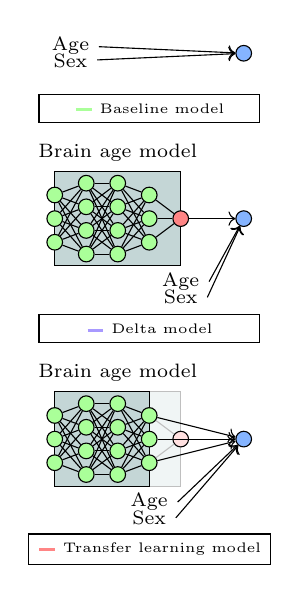
\begin{tikzpicture}
				\def\nodesize{2pt}
				\def\hsep{0.3}
				\def\vsep{0.4}
				\def\boxsize{2.8cm}

				\def\basey{9.6}
				\def\deltay{7.5}
				\def\transfery{4.7}
				\node [] (age) at (0.5 * \vsep, \basey + 0.1) {\scriptsize{Age}};
				\node [] (sex) at (0.5 * \vsep, \basey - 0.1) {\scriptsize{Sex}};
				\node [circle,draw=black,fill=prediction, inner sep=\nodesize] (pred) at (6 * \vsep,\basey) {};

				\path [->,draw=black] (age) -- (pred) {};
				\path [->,draw=black] (sex) -- (pred) {};
				\node [font=\tiny,draw=black,minimum width=\boxsize] at (3 * \vsep, \basey - 0.7) {\adjustbox{valign=c}{\tikz \draw[base, very thick] (0,0) -- (0.2,0);} Baseline model};

			\node [rectangle, draw=black,minimum height=1.2cm,minimum width=1.6cm,label=\scriptsize{Brain age model},fill=model] at (2 * \vsep,\deltay) {};
				\node [circle, draw=black,fill=nodes, inner sep=\nodesize] (00) at (0,\deltay - \hsep) {};
				\node [circle, draw=black,fill=nodes, inner sep=\nodesize] (01) at (0,\deltay) {};
				\node [circle, draw=black,fill=nodes, inner sep=\nodesize] (02) at (0,\deltay + \hsep) {};
				\node [circle, draw=black,fill=nodes, inner sep=\nodesize] (10) at (\vsep,\deltay - 1.5 * \hsep) {};
				\node [circle, draw=black,fill=nodes, inner sep=\nodesize] (11) at (\vsep,\deltay - 0.5 * \hsep) {};
				\node [circle, draw=black,fill=nodes, inner sep=\nodesize] (12) at (\vsep,\deltay + 0.5 * \hsep) {};
				\node [circle, draw=black,fill=nodes, inner sep=\nodesize] (13) at (\vsep,\deltay + 1.5 * \hsep) {};
				\node [circle, draw=black,fill=nodes, inner sep=\nodesize] (20) at (2 * \vsep,\deltay - 1.5 * \hsep) {};
				\node [circle, draw=black,fill=nodes, inner sep=\nodesize] (21) at (2 * \vsep,\deltay - 0.5 * \hsep) {};
				\node [circle, draw=black,fill=nodes, inner sep=\nodesize] (22) at (2 * \vsep,\deltay + 0.5 * \hsep) {};
				\node [circle, draw=black,fill=nodes, inner sep=\nodesize] (23) at (2 * \vsep,\deltay + 1.5 * \hsep) {};
				\node [circle, draw=black,fill=nodes, inner sep=\nodesize] (30) at (3 * \vsep,\deltay -  \hsep) {};
				\node [circle, draw=black,fill=nodes, inner sep=\nodesize] (31) at (3 * \vsep,\deltay) {};
				\node [circle, draw=black,fill=nodes, inner sep=\nodesize] (32) at (3 * \vsep,\deltay + \hsep) {};
				\node [circle, draw=black,fill=delta, inner sep=\nodesize] (40) at (4 * \vsep,\deltay) {};

				\node [draw=none] (age) at (4 * \vsep,\deltay - 0.8) {\scriptsize{Age}};
				\node [draw=none] (sex) at (4 * \vsep,\deltay - 1.0) {\scriptsize{Sex}};

				\node [circle,draw=black,fill=prediction, inner sep=\nodesize] (pred) at (6 * \vsep,\deltay) {};

				\path [-,draw=black] (00) -- (10) {};
				\path [-,draw=black] (00) -- (11) {};
				\path [-,draw=black] (00) -- (12) {};
				\path [-,draw=black] (00) -- (13) {};
				\path [-,draw=black] (01) -- (10) {};
				\path [-,draw=black] (01) -- (11) {};
				\path [-,draw=black] (01) -- (12) {};
				\path [-,draw=black] (01) -- (13) {};
				\path [-,draw=black] (02) -- (10) {};
				\path [-,draw=black] (02) -- (11) {};
				\path [-,draw=black] (02) -- (12) {};
				\path [-,draw=black] (02) -- (13) {};

				\path [-,draw=black] (10) -- (20) {};
				\path [-,draw=black] (10) -- (21) {};
				\path [-,draw=black] (10) -- (22) {};
				\path [-,draw=black] (10) -- (23) {};
				\path [-,draw=black] (11) -- (20) {};
				\path [-,draw=black] (11) -- (21) {};
				\path [-,draw=black] (11) -- (22) {};
				\path [-,draw=black] (11) -- (23) {};
				\path [-,draw=black] (12) -- (20) {};
				\path [-,draw=black] (12) -- (21) {};
				\path [-,draw=black] (12) -- (22) {};
				\path [-,draw=black] (12) -- (23) {};
				\path [-,draw=black] (13) -- (20) {};
				\path [-,draw=black] (13) -- (21) {};
				\path [-,draw=black] (13) -- (22) {};
				\path [-,draw=black] (13) -- (23) {};

				\path [-,draw=black] (20) -- (30) {};
				\path [-,draw=black] (20) -- (31) {};
				\path [-,draw=black] (20) -- (32) {};
				\path [-,draw=black] (21) -- (30) {};
				\path [-,draw=black] (21) -- (31) {};
				\path [-,draw=black] (21) -- (32) {};
				\path [-,draw=black] (22) -- (30) {};
				\path [-,draw=black] (22) -- (31) {};
				\path [-,draw=black] (22) -- (32) {};
				\path [-,draw=black] (23) -- (30) {};
				\path [-,draw=black] (23) -- (31) {};
				\path [-,draw=black] (23) -- (32) {};

				\path [-,draw=black] (30) -- (40) {};
				\path [-,draw=black] (31) -- (40) {};
				\path [-,draw=black] (32) -- (40) {};

				\path [-> ,draw=black] (40) -- (pred) {};
				\path [->,draw=black] (sex.east) -- (pred) {};
				\path [->,draw=black] (age.east) -- (pred) {};

				\node [font=\tiny,draw=black,minimum width=\boxsize] at (3 * \vsep, \deltay - 1.4) {\adjustbox{valign=c}{\tikz \draw[lasso, very thick] (0,0) -- (0.2,0);} Delta model};


				\node [rectangle, draw=black!25,minimum height=1.2cm,minimum width=1.6cm,label=\scriptsize{Brain age model},fill=model!25] at (2 * \vsep,\transfery) {};
				\node [rectangle, draw=black,minimum height=1.2cm,minimum width=1.2cm,fill=model] at (1.5 * \vsep, \transfery) {};
				\node [circle, draw=black,fill=nodes, inner sep=\nodesize] (00) at (0,\transfery - \hsep) {};
				\node [circle, draw=black,fill=nodes, inner sep=\nodesize] (01) at (0,\transfery) {};
				\node [circle, draw=black,fill=nodes, inner sep=\nodesize] (02) at (0,\transfery + \hsep) {};
				\node [circle, draw=black,fill=nodes, inner sep=\nodesize] (10) at (\vsep,\transfery - 1.5 * \hsep) {};
				\node [circle, draw=black,fill=nodes, inner sep=\nodesize] (11) at (\vsep,\transfery - 0.5 * \hsep) {};
				\node [circle, draw=black,fill=nodes, inner sep=\nodesize] (12) at (\vsep,\transfery + 0.5 * \hsep) {};
				\node [circle, draw=black,fill=nodes, inner sep=\nodesize] (13) at (\vsep,\transfery + 1.5 * \hsep) {};
				\node [circle, draw=black,fill=nodes, inner sep=\nodesize] (20) at (2 * \vsep,\transfery - 1.5 * \hsep) {};
				\node [circle, draw=black,fill=nodes, inner sep=\nodesize] (21)  at (2 * \vsep,\transfery - 0.5 * \hsep) {};
				\node [circle, draw=black,fill=nodes, inner sep=\nodesize] (22)  at (2 * \vsep,\transfery + 0.5 * \hsep) {};
				\node [circle, draw=black,fill=nodes, inner sep=\nodesize] (23)  at (2 * \vsep,\transfery + 1.5 * \hsep) {};
				\node [circle, draw=black,fill=nodes, inner sep=\nodesize] (30)  at (3 * \vsep,\transfery - \hsep) {};
				\node [circle, draw=black,fill=nodes, inner sep=\nodesize] (31)  at (3 * \vsep,\transfery) {};
				\node [circle, draw=black,fill=nodes, inner sep=\nodesize] (32)  at (3 * \vsep,\transfery + \hsep) {};
				\node [circle, draw=black,fill=delta!25, inner sep=\nodesize] (40)  at (4 * \vsep,\transfery) {};

				\node [draw=none] (age) at (3 * \vsep, \transfery - 0.8) {\scriptsize{Age}};
				\node [draw=none] (sex) at (3 * \vsep, \transfery - 1.0) {\scriptsize{Sex}};

				\node [circle,draw=black,fill=prediction, inner sep=\nodesize] (pred) at (6 * \vsep,\transfery) {};

				\path [-,draw=black] (00) -- (10) {};
				\path [-,draw=black] (00) -- (11) {};
				\path [-,draw=black] (00) -- (12) {};
				\path [-,draw=black] (00) -- (13) {};
				\path [-,draw=black] (01) -- (10) {};
				\path [-,draw=black] (01) -- (11) {};
				\path [-,draw=black] (01) -- (12) {};
				\path [-,draw=black] (01) -- (13) {};
				\path [-,draw=black] (02) -- (10) {};
				\path [-,draw=black] (02) -- (11) {};
				\path [-,draw=black] (02) -- (12) {};
				\path [-,draw=black] (02) -- (13) {};

				\path [-,draw=black] (10) -- (20) {};
				\path [-,draw=black] (10) -- (21) {};
				\path [-,draw=black] (10) -- (22) {};
				\path [-,draw=black] (10) -- (23) {};
				\path [-,draw=black] (11) -- (20) {};
				\path [-,draw=black] (11) -- (21) {};
				\path [-,draw=black] (11) -- (22) {};
				\path [-,draw=black] (11) -- (23) {};
				\path [-,draw=black] (12) -- (20) {};
				\path [-,draw=black] (12) -- (21) {};
				\path [-,draw=black] (12) -- (22) {};
				\path [-,draw=black] (12) -- (23) {};
				\path [-,draw=black] (13) -- (20) {};
				\path [-,draw=black] (13) -- (21) {};
				\path [-,draw=black] (13) -- (22) {};
				\path [-,draw=black] (13) -- (23) {};

				\path [-,draw=black] (20) -- (30) {};
				\path [-,draw=black] (20) -- (31) {};
				\path [-,draw=black] (20) -- (32) {};
				\path [-,draw=black] (21) -- (30) {};
				\path [-,draw=black] (21) -- (31) {};
				\path [-,draw=black] (21) -- (32) {};
				\path [-,draw=black] (22) -- (30) {};
				\path [-,draw=black] (22) -- (31) {};
				\path [-,draw=black] (22) -- (32) {};
				\path [-,draw=black] (23) -- (30) {};
				\path [-,draw=black] (23) -- (31) {};
				\path [-,draw=black] (23) -- (32) {};

				\path [-,draw=black!25] (30) -- (40) {};
				\path [-,draw=black!25] (31) -- (40) {};
				\path [-,draw=black!25] (32) -- (40) {};

				\path [-> ,draw=black] (30) -- (pred) {};
				\path [-> ,draw=black] (31) -- (pred) {};
				\path [-> ,draw=black] (32) -- (pred) {};
				\path [->,draw=black] (sex.east) -- (pred) {};
				\path [->,draw=black] (age.east) -- (pred) {};

				\node [font=\tiny,draw=black,minimum width=\boxsize] at (3 * \vsep, \transfery - 1.4) {\adjustbox{valign=c}{\tikz \draw[features, very thick] (0,0) -- (0.2,0);} Transfer learning model};
			\end{tikzpicture}
		\end{minipage}
		\begin{minipage}{0.59\textwidth}
			\begin{tikzpicture}
				\newcommand \ymin {-1.2}
				\newcommand \ymax {1.2}

				\begin{groupplot}[
					group style={
						group size=3 by 3,
						horizontal sep=0.25cm,
						vertical sep=0.25cm
					},
					height=0.55\textwidth,
					width=0.55\textwidth
				]
					\nextgroupplot[
						xmin=0,
						xmax=1,
						ymin=0,
						ymax=1,
						xticklabels={,,},
						yticklabels={,,},
						ticks=none
					]

					\addplot [black] coordinates {(0,0) (1,1)};
					\addplot [base,very thick] table [x=fpr,y=tpr] {\MSbaselineroc};\label{trace:baseline}
					\addplot [lasso,very thick] table [x=fpr,y=tpr] {\MSdeltaroc};\label{trace:delta}
					\addplot [features,very thick] table [x=fpr,y=tpr] {\MSfeaturesroc};\label{trace:features}

					\coordinate (MS) at (axis cs:1,0) {};

					\node [anchor=north west] at (axis cs: 0,1) {\textbf{\footnotesize{MS}}};

					\nextgroupplot[
						xmin=0,
						xmax=1,
						ymin=0,
						ymax=1,
						xticklabels={,,},
						yticklabels={,,},
						ticks=none
					]

					\addplot [black] coordinates {(0,0) (1,1)};
					\addplot [base,very thick] table [x=fpr,y=tpr] {\ADbaselineroc};
					\addplot [lasso,very thick] table [x=fpr,y=tpr] {\ADdeltaroc};
					\addplot [features,very thick] table [x=fpr,y=tpr] {\ADfeaturesroc};

					\coordinate (AD) at (axis cs:1,0) {};

					\node [anchor=north west] at (axis cs: 0,1) {\textbf{\footnotesize{AD}}};

					\nextgroupplot[
						xmin=0,
						xmax=1,
						ymin=0,
						ymax=1,
						xticklabels={,,},
						yticklabels={,,},
						ticks=none
					]

					\addplot [black] coordinates {(0,0) (1,1)};
					\addplot [base,very thick] table [x=fpr,y=tpr] {\MCIbaselineroc};
					\addplot [lasso,very thick] table [x=fpr,y=tpr] {\MCIdeltaroc};
					\addplot [features,very thick] table [x=fpr,y=tpr] {\MCIfeaturesroc};

					\coordinate (MCI) at (axis cs:1,0) {};

					\node [anchor=north west] at (axis cs: 0,1) {\textbf{\footnotesize{MCI}}};

					\nextgroupplot[
						xmin=0,
						xmax=1,
						ymin=0,
						ymax=1,
						xticklabels={,,},
						yticklabels={,,},
						ticks=none
					]

					\addplot [black] coordinates {(0,0) (1,1)};
					\addplot [base,very thick] table [x=fpr,y=tpr] {\SCZbaselineroc};
					\addplot [lasso,very thick] table [x=fpr,y=tpr] {\SCZdeltaroc};
					\addplot [features,very thick] table [x=fpr,y=tpr] {\SCZfeaturesroc};

					\coordinate (SCZ) at (axis cs:1,0) {};

					\node [anchor=north west] at (axis cs: 0,1) {\textbf{\footnotesize{SCZ}}};

					\nextgroupplot[
						xmin=0,
						xmax=1,
						ymin=0,
						ymax=1,
						xticklabels={,,},
						yticklabels={,,},
						ticks=none
					]

					\addplot [black] coordinates {(0,0) (1,1)};
					\addplot [base,very thick] table [x=fpr,y=tpr] {\PSYbaselineroc};
					\addplot [lasso,very thick] table [x=fpr,y=tpr] {\PSYdeltaroc};
					\addplot [features,very thick] table [x=fpr,y=tpr] {\PSYfeaturesroc};

					\coordinate (PSY) at (axis cs:1,0) {};

					\node [anchor=north west] at (axis cs: 0,1) {\textbf{\footnotesize{PSY}}};

					\nextgroupplot[
						xmin=0,
						xmax=1,
						ymin=0,
						ymax=1,
						xticklabels={,,},
						yticklabels={,,},
						ticks=none
					]

					\addplot [black] coordinates {(0,0) (1,1)};
					\addplot [base,very thick] table [x=fpr,y=tpr] {\MOODbaselineroc};
					\addplot [lasso,very thick] table [x=fpr,y=tpr] {\MOODdeltaroc};
					\addplot [features,very thick] table [x=fpr,y=tpr] {\MOODfeaturesroc};

					\coordinate (MOOD) at (axis cs:1,0) {};

					\node [anchor=north west] at (axis cs: 0,1) {\textbf{\footnotesize{MOOD}}};

				\end{groupplot}

				\matrix [
					matrix of nodes,
					draw=none,
					row sep=-0.15cm,
					column sep=-0.2cm,
					anchor=south east,
					column 2/.style={nodes={font=\tiny}},
					outer sep=-2pt,
					ampersand replacement=\&
				] at (MS) {
					\&\underline{AUC}\\
					\adjustbox{valign=c}{\tikz \draw[base, very thick] (0,0) -- (0.2,0);}\&0.50\\
					\adjustbox{valign=c}{\tikz \draw[lasso, very thick] (0,0) -- (0.2,0);}\&0.71\\
					\adjustbox{valign=c}{\tikz \draw[features, very thick] (0,0) -- (0.2,0);}\&0.79\\
				};

				\matrix [
					matrix of nodes,
					draw=none,
					row sep=-0.15cm,
					column sep=-0.2cm,
					anchor=south east,
					column 2/.style={nodes={font=\tiny}},
					outer sep=-2pt,
					ampersand replacement=\&
				] at (AD) {
					\&\underline{AUC}\\
					\adjustbox{valign=c}{\tikz \draw[base, very thick] (0,0) -- (0.2,0);}\&0.51\\
					\adjustbox{valign=c}{\tikz \draw[lasso, very thick] (0,0) -- (0.2,0);}\&0.69\\
					\adjustbox{valign=c}{\tikz \draw[features, very thick] (0,0) -- (0.2,0);}\&0.83\\
				};

				\matrix [
					matrix of nodes,
					draw=none,
					row sep=-0.15cm,
					column sep=-0.2cm,
					anchor=south east,
					column 2/.style={nodes={font=\tiny}},
					outer sep=-2pt,
					ampersand replacement=\&
				] at (MCI) {
					\&\underline{AUC}\\
					\adjustbox{valign=c}{\tikz \draw[base, very thick] (0,0) -- (0.2,0);}\&0.54\\
					\adjustbox{valign=c}{\tikz \draw[lasso, very thick] (0,0) -- (0.2,0);}\&0.65\\
					\adjustbox{valign=c}{\tikz \draw[features, very thick] (0,0) -- (0.2,0);}\&0.73\\
				};

				\matrix [
					matrix of nodes,
					draw=none,
					row sep=-0.15cm,
					column sep=-0.2cm,
					anchor=south east,
					column 2/.style={nodes={font=\tiny}},
					outer sep=-2pt,
					ampersand replacement=\&
				] at (SCZ) {
					\&\underline{AUC}\\
					\adjustbox{valign=c}{\tikz \draw[base, very thick] (0,0) -- (0.2,0);}\&0.50\\
					\adjustbox{valign=c}{\tikz \draw[lasso, very thick] (0,0) -- (0.2,0);}\&0.58\\
					\adjustbox{valign=c}{\tikz \draw[features, very thick] (0,0) -- (0.2,0);}\&0.62\\
				};

				\matrix [
					matrix of nodes,
					draw=none,
					row sep=-0.15cm,
					column sep=-0.2cm,
					anchor=south east,
					column 2/.style={nodes={font=\tiny}},
					outer sep=-2pt,
					ampersand replacement=\&
				] at (PSY) {
					\&\underline{AUC}\\
					\adjustbox{valign=c}{\tikz \draw[base, very thick] (0,0) -- (0.2,0);}\&0.47\\
					\adjustbox{valign=c}{\tikz \draw[lasso, very thick] (0,0) -- (0.2,0);}\&0.52\\
					\adjustbox{valign=c}{\tikz \draw[features, very thick] (0,0) -- (0.2,0);}\&0.62\\
				};

				\matrix [
					matrix of nodes,
					draw=none,
					row sep=-0.15cm,
					column sep=-0.2cm,
					anchor=south east,
					column 2/.style={nodes={font=\tiny}},
					outer sep=-2pt,
					ampersand replacement=\&
				] at (MOOD) {
					\&\underline{AUC}\\
					\adjustbox{valign=c}{\tikz \draw[base, very thick] (0,0) -- (0.2,0);}\&0.52\\
					\adjustbox{valign=c}{\tikz \draw[lasso, very thick] (0,0) -- (0.2,0);}\&0.55\\
					\adjustbox{valign=c}{\tikz \draw[features, very thick] (0,0) -- (0.2,0);}\&0.59\\
				};

			\end{tikzpicture}
		\end{minipage}
	\end{frame}

	\begin{frame}{Paper 2: Genetic architecture of brain age}
		\centering
		\vfill
		\begin{tikzpicture}
			\node[inner sep=1pt, fill=white, draw=black] {
				
\includegraphics[width=8cm]{data/paper2.png}
			};
		\end{tikzpicture}
		\vfill
	\end{frame}

	\begin{frame}{Paper 2: Genetic architecture of brain age}
		\centering
		\vfill
		\begin{tikzpicture}
			\node[inner sep=1pt, fill=white, draw=black] {
				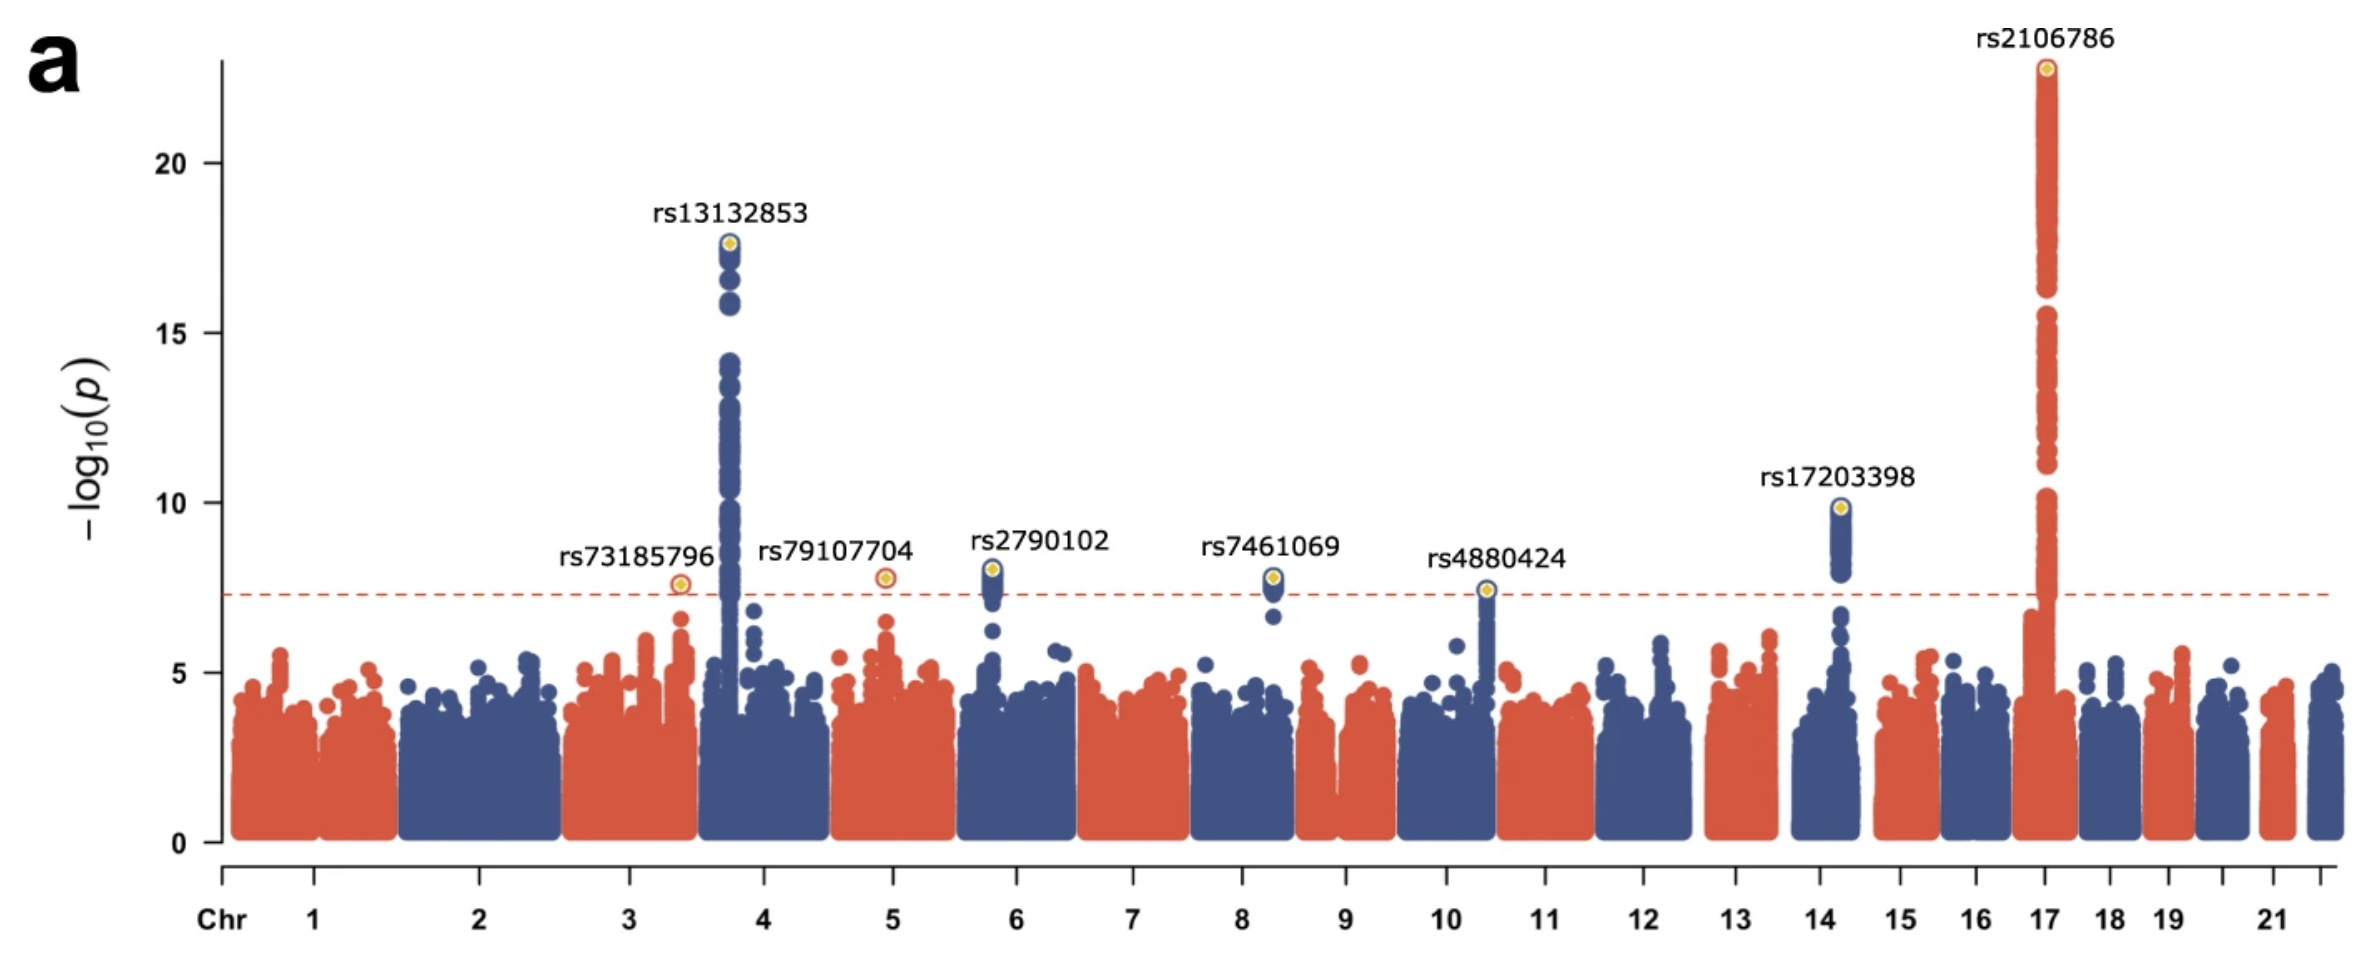
\includegraphics[width=10cm]{data/gwas.png}
			};
		\end{tikzpicture}
		\vfill
	\end{frame}

	\begin{frame}{Paper 2: Genetic architecture of brain age}
		\centering
		\vfill
		\begin{tikzpicture}
			\node[inner sep=1pt, fill=white, draw=black] {
				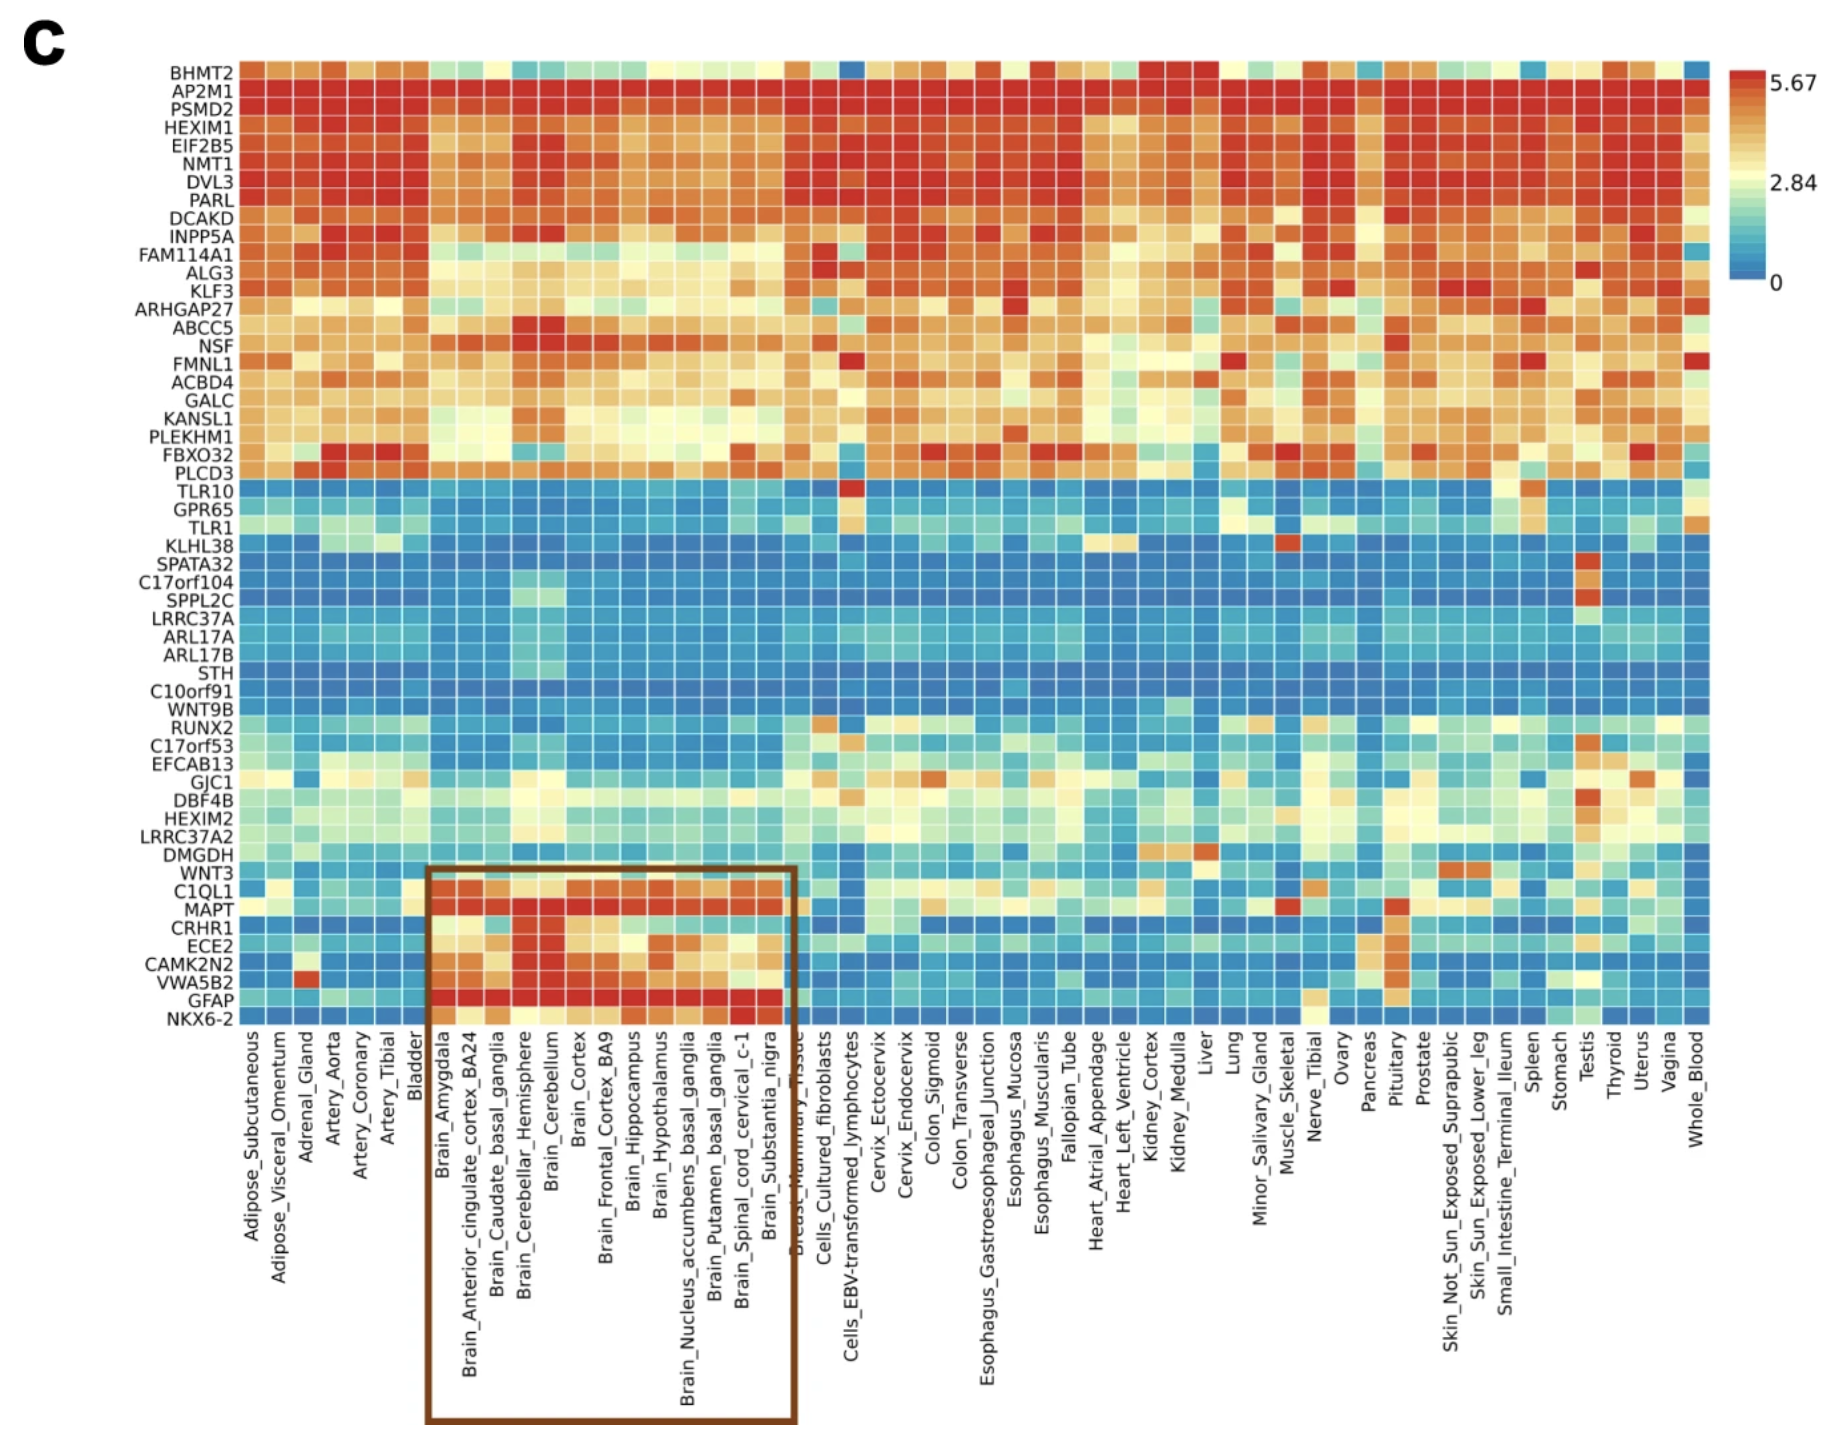
\includegraphics[width=8cm]{data/expression.png}
			};
		\end{tikzpicture}
		\vfill
	\end{frame}

	\begin{frame}{Paper 2: Genetic architecture of brain age}
		\centering
		\vfill
		\begin{tikzpicture}
			\node[inner sep=1pt, fill=white, draw=black] {
				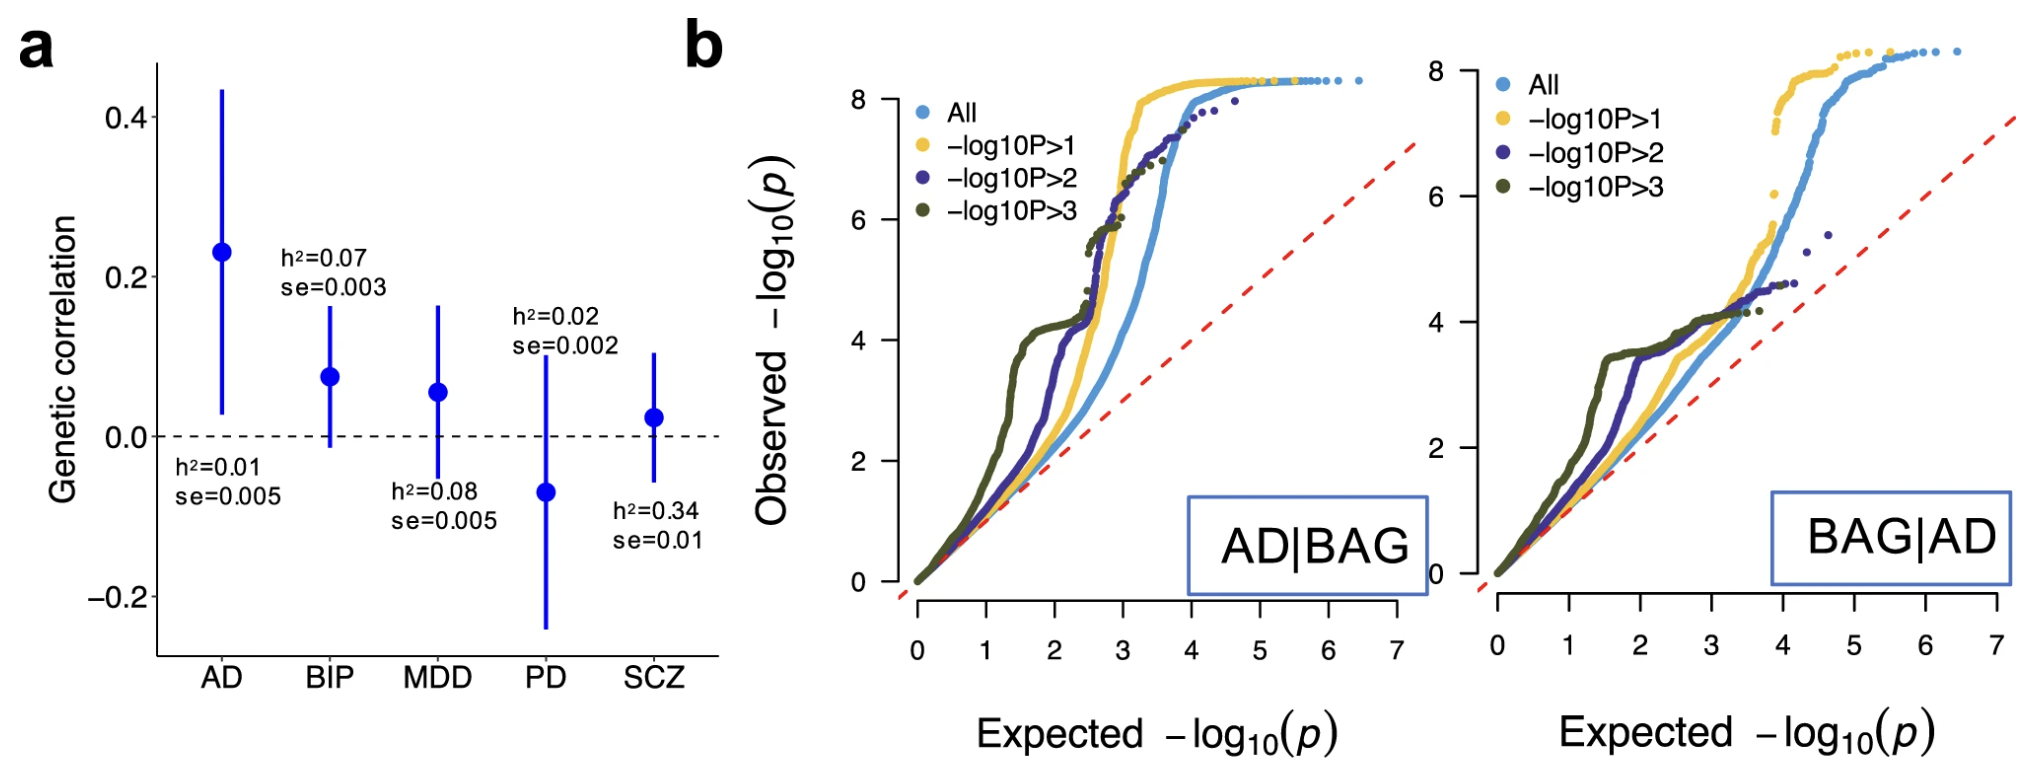
\includegraphics[width=10.5cm]{data/correlation.png}
			};
		\end{tikzpicture}
		\vfill
	\end{frame}

	\begin{frame}{Paper 2: Genetic architecture of brain age}
		\centering
		\vfill
		\begin{tikzpicture}
			\node[inner sep=1pt, fill=white, draw=black] {
				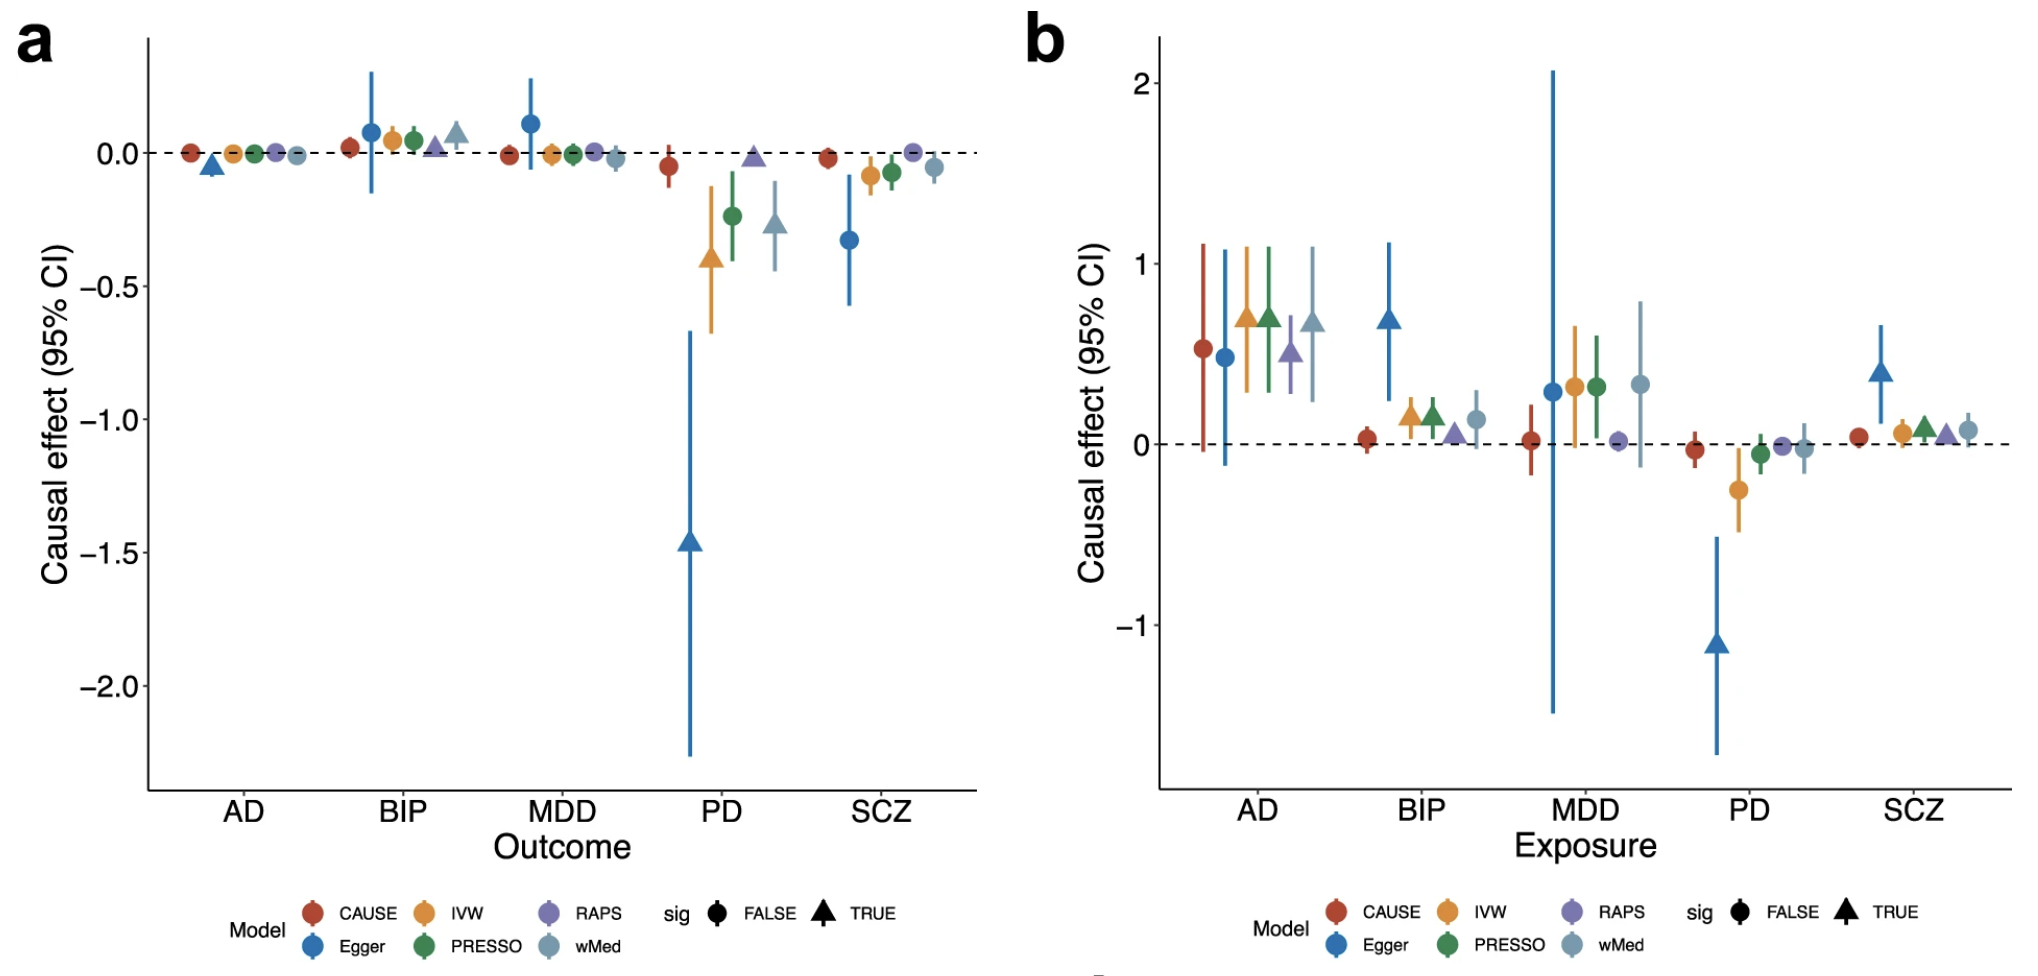
\includegraphics[width=10.5cm]{data/causality.png}
			};
		\end{tikzpicture}
		\vfill
	\end{frame}

	\begin{frame}{Paper 3: Explainable AI and dementia} % Frontpage
		\centering
		\vfill
		\begin{tikzpicture}
			\node[inner sep=1pt, fill=white, draw=black] {
				
\includegraphics[width=8cm]{data/paper3.png}
			};
		\end{tikzpicture}
		\vfill
	\end{frame}

	\begin{frame}{Paper 3: Explainable AI and dementia} % Dataset
		\pgfplotstableread[col sep=comma]{data/dementia_dataset/dementia_full.csv}\dementiafull
		\pgfplotstableread[col sep=comma]{data/dementia_dataset/dementia_addneuromed_GE_MEDICAL_SYSTEMS.csv}\dementiage
		\pgfplotstableread[col sep=comma]{data/dementia_dataset/dementia_addneuromed_PICKER_International_Inc.csv}\dementiapicker
		\pgfplotstableread[col sep=comma]{data/dementia_dataset/dementia_ADNI_15T.csv}\dementiaadnione
		\pgfplotstableread[col sep=comma]{data/dementia_dataset/dementia_ADNI_30T.csv}\dementiaadnithree
		\pgfplotstableread[col sep=comma]{data/dementia_dataset/dementia_AIBL_10.csv}\dementiaaiblone
		\pgfplotstableread[col sep=comma]{data/dementia_dataset/dementia_AIBL_20.csv}\dementiaaibltwo
		\pgfplotstableread[col sep=comma]{data/dementia_dataset/dementia_miriad_15_T_Signa.csv}\dementiamiriad
		\pgfplotstableread[col sep=comma]{data/dementia_dataset/dementia_oasis3_15T.csv}\dementiaoasisone
		\pgfplotstableread[col sep=comma]{data/dementia_dataset/dementia_oasis3_30T.csv}\dementiaoasisthree
		\pgfplotstableread[col sep=comma]{data/dementia_dataset/dementia_Oslo_GE750.csv}\dementiaoslo
		\pgfplotstableread[col sep=comma]{data/dementia_dataset/dementia_timepoints.csv}\dementiatimepoints

		\def\xmin{46}
		\def\xmax{99}
		\def\ymin{-1.4}
		\def\ymax{1.2}

		\centering
		\vfill
		\begin{tikzpicture}
            \begin{axis}[
                width=\textwidth,
                height=0.45\textwidth,
                xmin=\xmin,
                xmax=\xmax,
                ymin=-1.6,
                ymax=\ymax,
                xtick={55,60,65,70,75,80,85,90,95},
				axis lines=center,
				axis y line=none,
				clip=false
            ]
                \addplot[name path=zero, draw=none] coordinates {(47,0) (97,0)};
                \addplot[name path=fcases, draw=cases-default, very thick] table [x=x, y=F-cases]{\dementiafull};\label{trace:cases}
                \addplot[fill=cases-default, opacity=0.2] fill between [of=zero and fcases];
                \addplot[name path=fcontrols, draw=controls-default, very thick] table [x=x, y=F-controls]{\dementiafull};\label{trace:controls}
                \addplot[fill=controls-default, opacity=0.2] fill between [of=zero and fcontrols];
                \addplot[name path=mcases, draw=cases-default, very thick] table [x=x,y expr=\thisrow{M-cases} * -1]{\dementiafull};
                \addplot[fill=cases-default, opacity=0.2] fill between [of=zero and mcases];
                \addplot[name path=mcontrols, draw=controls-default, very thick] table [x=x,y expr=\thisrow{M-controls} * -1]{\dementiafull};
                \addplot[fill=controls-default, opacity=0.2] fill between [of=zero and mcontrols];
                \node[anchor=south west] at (axis cs: 46, 0.07) {\textbf{FEMALE}};
                \node[anchor=north west] at (axis cs: 46, -0.07) {\textbf{MALE}};
                \node[anchor=south, align=center] (n) at (axis cs: 72.5,-1.6) {n=1708};
                \node[anchor=north,font=\footnotesize] at ($(n.south) + (0,-2.5) $) {\ref{trace:controls} Controls\hspace{0.3cm}\ref{trace:cases} Cases};
            \end{axis}
        \end{tikzpicture}
		\vspace{-0.1cm}

			\newcommand{\scannersubplot}[3]{
				\nextgroupplot[
						axis lines=center,
						axis y line=none,
						xmin=\xmin,
						xmax=\xmax,
						ymin=\ymin - 0.25,
						ymax=\ymax + 0.25,
						xmajorticks=false,
						axis line style={-}
					]

						\addplot[name path=zero, draw=none] coordinates {(\xmin,0) (\xmax,0)};
						\addplot[name path=fcases, draw=cases-default, very thick] table [x=x, y=F-cases]{####1};
						\addplot[fill=cases-default, opacity=0.2] fill between [of=zero and fcases];
						\addplot[name path=fcontrols, draw=controls-default, very thick] table [x=x, y=F-controls]{####1};
						\addplot[fill=controls-default, opacity=0.2] fill between [of=zero and fcontrols];
						\addplot[name path=mcases, draw=cases-default, very thick] table [x=x,y expr=\thisrow{M-cases} * -1]{####1};
						\addplot[fill=cases-default, opacity=0.2] fill between [of=zero and mcases];
						\addplot[name path=mcontrols, draw=controls-default, very thick] table [x=x,y expr=\thisrow{M-controls} * -1]{####1};
						\addplot[fill=controls-default, opacity=0.2] fill between [of=zero and mcontrols];
						\node[anchor=south] at (axis cs: 72.5,1) {\tiny{####2}};
						\node[anchor=north] at (axis cs: 72.5,-1) {\tiny{\textbf{n=####3}}};
			}
			\begin{tikzpicture}
				\begin{groupplot}[
					group style={
						group size=5 by 2,
						horizontal sep=0.25cm,
						vertical sep=0.25cm
					},
					height=0.314\textwidth,
					width=0.314\textwidth
				]
					\scannersubplot{\dementiaadnithree}{ADNI 3.0T}{506}
					\scannersubplot{\dementiaoasisthree}{OASIS3 3.0T}{438}
					\scannersubplot{\dementiaadnione}{ADNI 1.5T}{290}
					\scannersubplot{\dementiaoslo}{Oslo GE750}{226}
					\scannersubplot{\dementiaaiblone}{AIBL Site 1}{92}
					\scannersubplot{\dementiage}{ANM GE}{74}
					\scannersubplot{\dementiamiriad}{MIRIAD}{38}
					\scannersubplot{\dementiaaibltwo}{AIBL Site 2}{22}
					\scannersubplot{\dementiapicker}{ANM Picker}{12}
					\scannersubplot{\dementiaoasisone}{OASIS3 1.5T}{10}
				\end{groupplot}
		\end{tikzpicture}

		\vfill
	\end{frame}

	\begin{frame}{Paper 3: Explainable AI and dementia} % Predictive performance
		\pgfplotstableread[col sep=comma]{data/test_distributions.csv}\testdistributions
		\pgfplotstableread[col sep=comma]{data/test_predictions.csv}\testpredictions

		\newcommand{\ymin}{-0.35}
		\newcommand{\ymax}{1.05}

		\begin{tikzpicture}
			\begin{axis}[
				name=distributions,
				height=0.4\textwidth,
				width=0.94\textwidth,
				xtick pos=bottom,
				ymajorticks=false,
				xmin=0,
				xmax=1,
				ymin=\ymin,
				ymax=\ymax,
				xlabel=\small{Prediction},
				every tick label/.append style={font=\footnotesize}
			]
				\addplot[name path=controls, draw=controls-default, very thick] table [x=prediction,y=controls]{\testdistributions};
				\addplot[name path=cases, draw=cases-default, very thick] table [x=prediction,y=cases]{\testdistributions};
				\addplot[name path=zero, draw=black] coordinates {(0,0) (1,0)};
				\addplot[fill=controls-default, opacity=0.2] fill between [of=zero and controls];
				\addplot[fill=cases-default, opacity=0.2] fill between [of=zero and cases];
				\addplot[
					scatter/classes={
						control={controls-default, draw=black, opacity=0.5},
						case={cases-default, draw=black, opacity=0.5}
					},
					scatter,
					mark=*,
					only marks,
					point meta=explicit symbolic
				] table [
					y expr=\thisrow{y} * -0.15 - 0.1,
					meta=class,
				] {\testpredictions};
				\addplot[dashed] coordinates {(0.5, \ymin) (0.5, \ymax)};
			\end{axis}
			% ONLY FOR ALIGNMENT
			\node[anchor=south east] at ($ (distributions.south west) + (0,0.28) $) {\textcolor{white}{\tiny{Controls}}};
			\node[anchor=south east] at ($ (distributions.south west) + (0,0.0) $) {\textcolor{white}{\tiny{Cases}}};

			\node[anchor=south west] at ($ (distributions.south east) + (0,0.28) $) {\tiny{Controls}};
			\node[anchor=south west] at ($ (distributions.south east) + (0,0.0) $) {\tiny{Cases}};
			\node[anchor=south,align=center] at (distributions.north) {\tiny{$t=0.5$}};
		\end{tikzpicture}

	\end{frame}

	\begin{frame}{Paper 3: Explainable AI and dementia} % Example relevance maps
		\centering
		\vfill
		\begin{tikzpicture}
			\node[
				minimum height=0.41\textwidth,
				minimum width=0.32\textwidth,
				fill=black
			] (box1) at (0, 0) {};
			\node[anchor=south] at (box1.south) {
				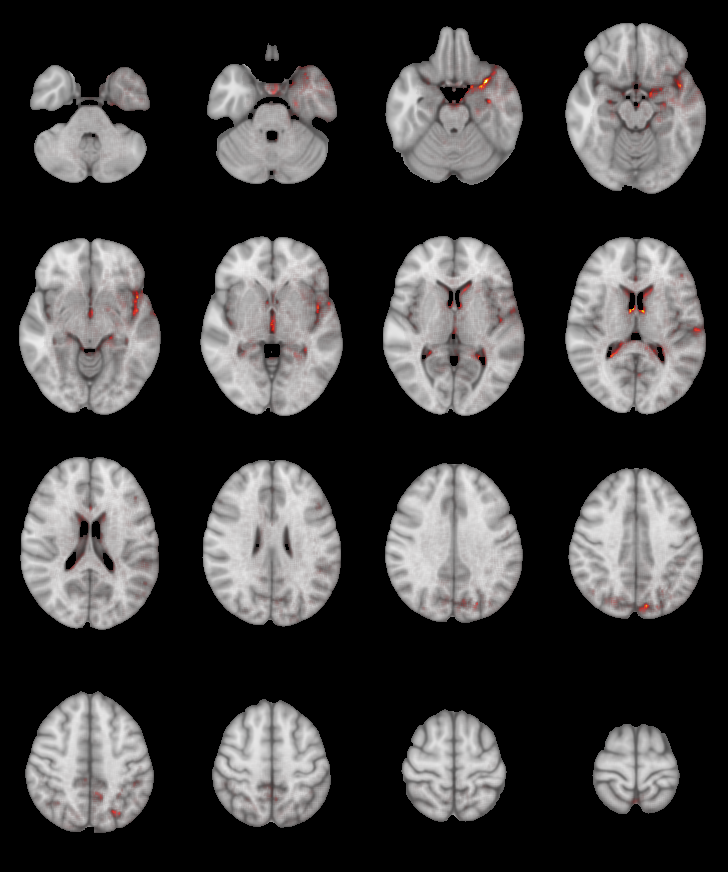
\includegraphics[width=0.31\textwidth]{data/subject1.png}
			};
			\node[anchor=north,inner sep=2pt, text=white, font=\footnotesize] at (box1.north) {Patient 1};

			\node
				[minimum height=0.41\textwidth,
				minimum width=0.32\textwidth,
				fill=black,
				anchor=west
			] (box2) at ($ (box1.east) + (0.05,0) $) {};
			\node[anchor=south] at (box2.south) {
				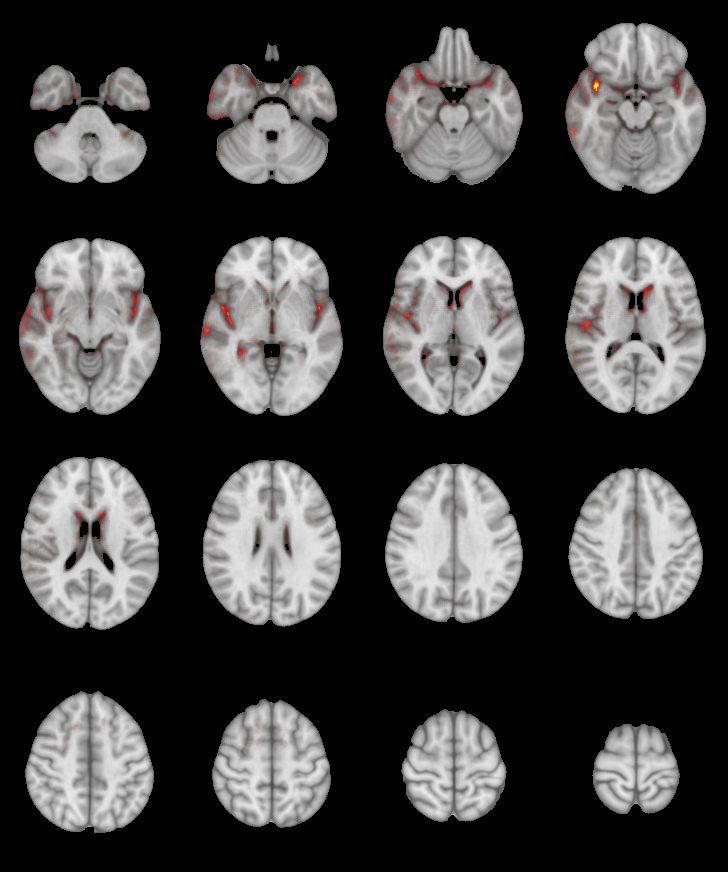
\includegraphics[width=0.31\textwidth]{data/subject2.png}
			};
			\node[anchor=north,inner sep=3pt, text=white, font=\footnotesize] at (box2.north) {Partient 2};

			\node
				[minimum height=0.41\textwidth,
				minimum width=0.32\textwidth,
				fill=black,
				anchor=west
			] (box3) at ($ (box2.east) + (0.05,0) $) {};
			\node[anchor=south] at (box3.south) {
				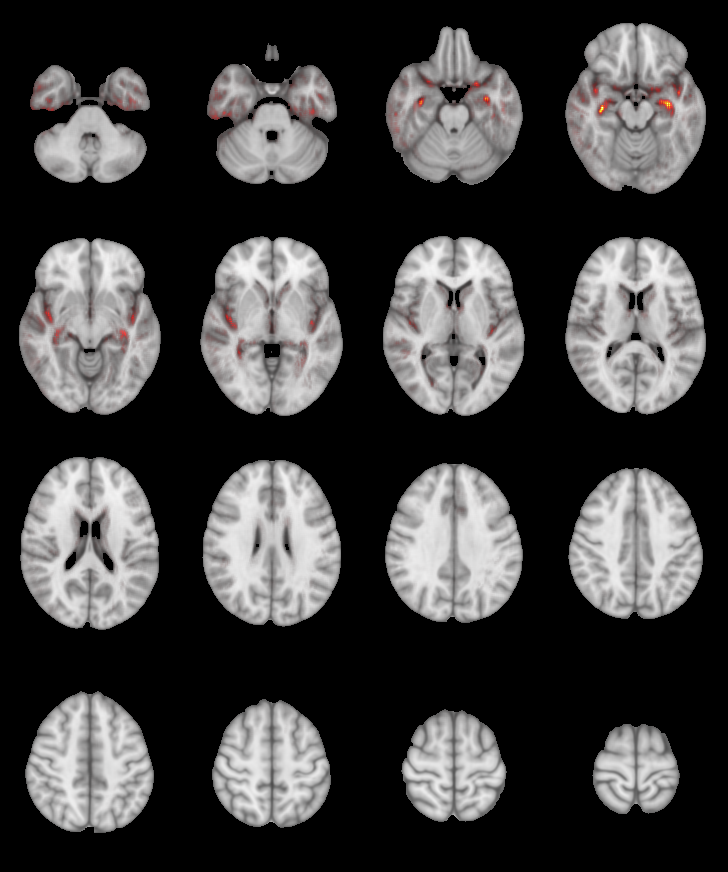
\includegraphics[width=0.31\textwidth]{data/subject3.png}
			};
			\node[anchor=north,inner sep=3pt, text=white, font=\footnotesize] at (box3.north) {Patient 3};

		\end{tikzpicture}
		\vfill
	\end{frame}

	\begin{frame}{Paper 3: Explainable AI and dementia} % Average maps
		\centering
		\vfill
		\begin{tikzpicture}
			\node[draw=none] at (-2, -2) {};
			\node[draw=none] at (6.5, 2.5) {};
			\node[label={[text depth=0]above:LRP}] at (0, 0) {
				
\includegraphics[width=0.31\textwidth]{data/dementia.png}
			};
		\end{tikzpicture}
		\vfill
	\end{frame}

	\begin{frame}{Paper 3: Explainable AI and dementia} % Average maps
		\centering
		\vfill
		\begin{tikzpicture}
			\node[draw=none] at (-2, -2) {};
			\node[draw=none] at (6.5, 2.5) {};
			\node[label={[text depth=0]above:LRP}] at (0, 0) {
				
\includegraphics[width=0.31\textwidth]{data/dementia.png}
			};

			\node[label={[text depth=0]above:GingerALE}] at (4.5, 0) {
				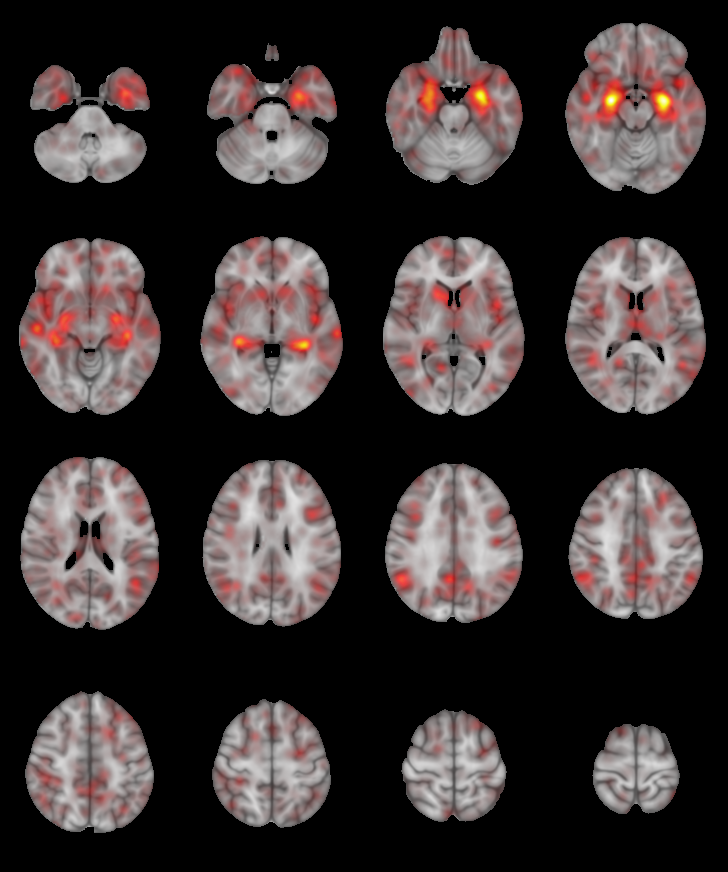
\includegraphics[width=0.31\textwidth]{data/ALE.png}
			};
		\end{tikzpicture}
		\vfill
	\end{frame}

	\begin{frame}{Paper 3: Explainable AI and dementia} % Overlap
		\centering
		\vfill
		\begin{tikzpicture}
            \node[
                minimum height=0.45\textwidth,
                minimum width=0.33\textwidth,
                fill=black
            ] (box1) at (0, 0) {};
            \node[anchor=south] at ($ (box1.south) + (0, 0.3) $) {
                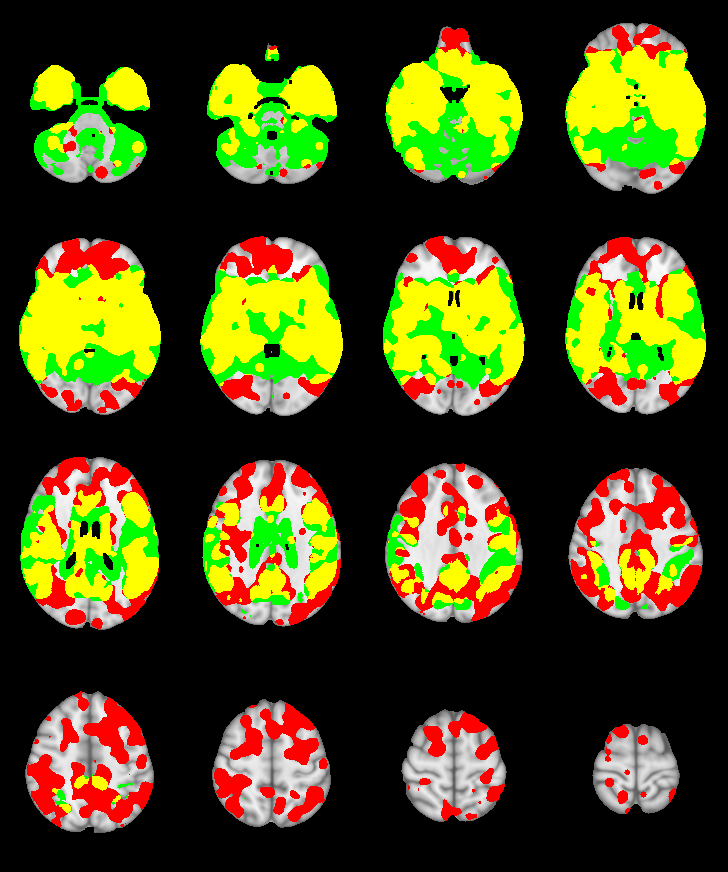
\includegraphics[width=0.31\textwidth]{data/test_50.png}
            };
            \node[anchor=north,inner sep=2pt, text=white, font=\footnotesize] at (box1.north) {50th percentile};

            \node
                [minimum height=0.45\textwidth,
                minimum width=0.33\textwidth,
                fill=black,
                anchor=west
            ] (box2) at ($ (box1.east) + (0.05,0) $) {};
            \node[anchor=south] at ($ (box2.south) + (0, 0.3) $) {
                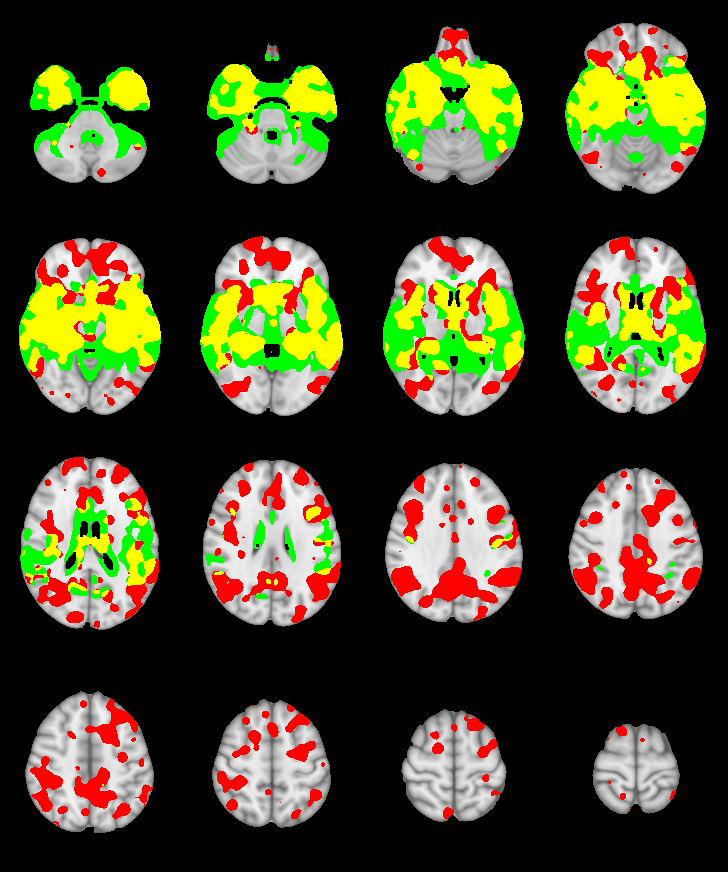
\includegraphics[width=0.31\textwidth]{data/test_70.png}
            };
            \node[anchor=north,inner sep=3pt, text=white, font=\footnotesize] at (box2.north) {70th percentile};

            \node
                [minimum height=0.45\textwidth,
                minimum width=0.33\textwidth,
                fill=black,
                anchor=west
            ] (box3) at ($ (box2.east) + (0.05,0) $) {};
            \node[anchor=south] at ($ (box3.south) + (0, 0.3) $) {
                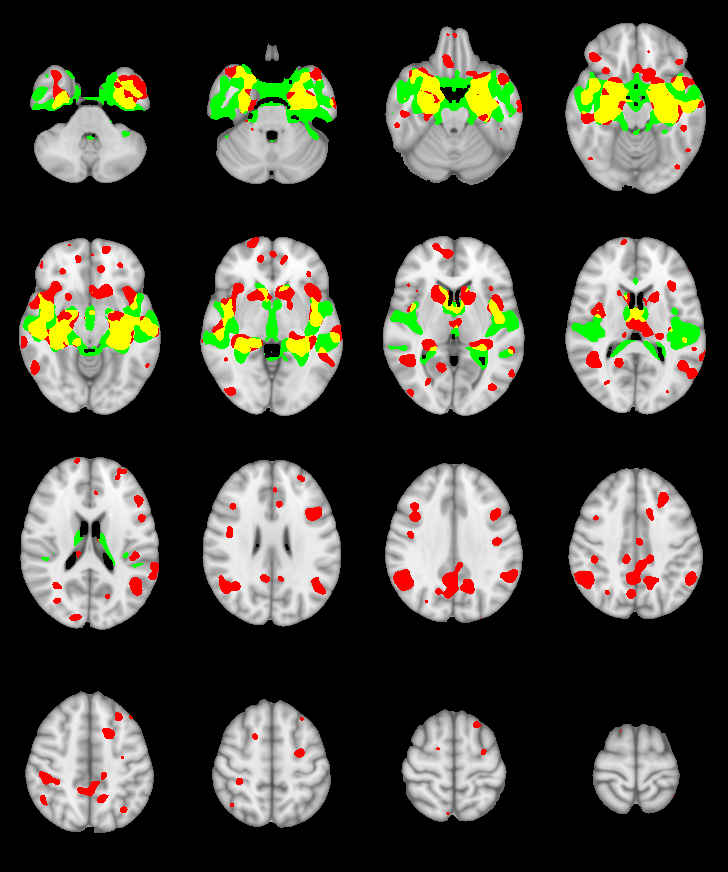
\includegraphics[width=0.31\textwidth]{data/test_90.png}
            };
            \node[anchor=north,inner sep=3pt, text=white, font=\footnotesize] at (box3.north) {90th percentile};

            \node[anchor=south, inner sep=0pt, text depth=0] (overlap) at ($ (box2.south) + (0.1, 0.15) $) {\textcolor{white}{\scriptsize{Overlap}}};
            \node[anchor=east, inner sep=2pt, fill=yellow] (overlap-box) at ($ (overlap.west) + (-0.07, 0) $) {};
            \node[anchor=east, inner sep=0pt,text depth=0] (lrp) at ($ (overlap-box.west) + (-0.2, 0) $) {\textcolor{white}{\scriptsize{LRP}}};
            \node[anchor=east, inner sep=2pt, fill=green] at ($ (lrp.west) + (-0.07, 0) $) {};
            \node[anchor=west, inner sep=2pt, fill=red] (ale-box) at ($ (overlap.east) + (0.2, 0) $) {};
            \node[anchor=west, inner sep=0pt, text depth=0] at ($ (ale-box.east) + (0.07, 0) $) {\textcolor{white}{\scriptsize{ALE}}};

        \end{tikzpicture}
		\vfill
	\end{frame}

	\begin{frame}{Paper 3: Explainable AI and dementia} % Components
		\centering
		\vfill
		\begin{tikzpicture}
			\newcommand{\drawmask}[3]{
				\node[anchor=west] (second) at (####2*0.89, ####3*-1) {
					\includegraphics[
						width=0.9cm,
						clip=true,
						trim = 192mm 232mm 0mm 0mm
					]{data/components/component_####1.png}
				};
			}
			\foreach \i in {0,...,7}{
				\foreach \j in {0,...,7}{
					\pgfmathsetmacro{\idx}{int(\i * 8 + \j)}
					\drawmask{\idx}{\j}{\i}
				}
			}
		\end{tikzpicture}
		\vfill
	\end{frame}

	\begin{frame}{Paper 3: Explainable AI and dementia} % Prognosis
		\centering
		\vfill
		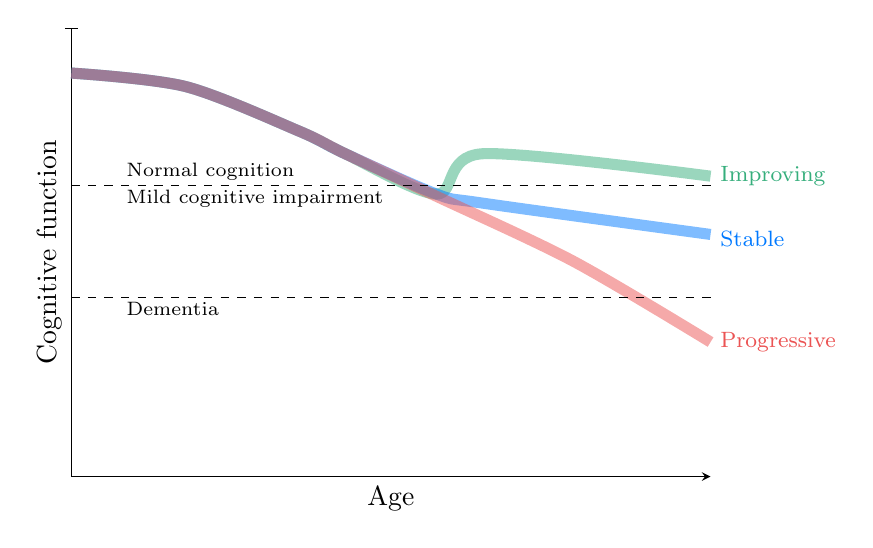
\begin{tikzpicture}
			\begin{axis}[
				height=0.6\textwidth,
				width=0.8\textwidth,
				xlabel={Age},
				ylabel={Cognitive function},
				ticks=none,
				axis x line=bottom,
				axis y line=left,
				y axis line style={-|},
				xmin=0,
				xmax=1.4,
				ymin=0,
				ymax=1,
				clip=false
			]
			\addplot[draw=healthy-default, smooth, line width=4pt, opacity=0.5] coordinates {
				(0, 0.9)
				(0.25, 0.87)
				(0.5, 0.77)
				(0.6, 0.72)
				(0.8, 0.63)
				(0.9, 0.72)
				(1.4, 0.67)
			};
			\addplot[draw=controls-default, smooth, line width=4pt, opacity=0.5] coordinates {
				(0, 0.9)
				(0.25, 0.87)
				(0.5, 0.77)
				(0.6, 0.72)
				(0.8, 0.63)
				(0.9, 0.61)
				(1.4, 0.54)
			};
			\addplot[draw=cases-default, smooth, line width=4pt, opacity=0.5] coordinates {
				(0, 0.9)
				(0.25, 0.87)
				(0.5, 0.77)
				(0.6, 0.72)
				(0.8, 0.625)
				(1.1, 0.48)
				(1.4, 0.3)
			};
			\addplot[dashed] coordinates {
				(0, 0.65)
				(1.4, 0.65)
			};
			\addplot[dashed] coordinates {
				(0, 0.4)
				(1.4, 0.4)
			};
			\node[anchor=south west] at (axis cs: 0.1, 0.64) {\scriptsize{Normal cognition}};
			\node[anchor=north west] at (axis cs: 0.1, 0.66) {\scriptsize{Mild cognitive impairment}};
			\node[anchor=north west] at (axis cs: 0.1, 0.41) {\scriptsize{Dementia}};
			\node[anchor=west] at (axis cs: 1.4, 0.67) {\textcolor{healthy-default}{\footnotesize{Improving}}};
			\node[anchor=west] at (axis cs: 1.4, 0.53) {\textcolor{controls-default}{\footnotesize{Stable}}};
			\node[anchor=west] at (axis cs: 1.4, 0.3) {\textcolor{cases-default}{\footnotesize{Progressive}}};
			\end{axis}
		\end{tikzpicture}
		\vfill
	\end{frame}

	\begin{frame}{Paper 3: Explainable AI and dementia} % Prognosis
		\centering
		\vfill
		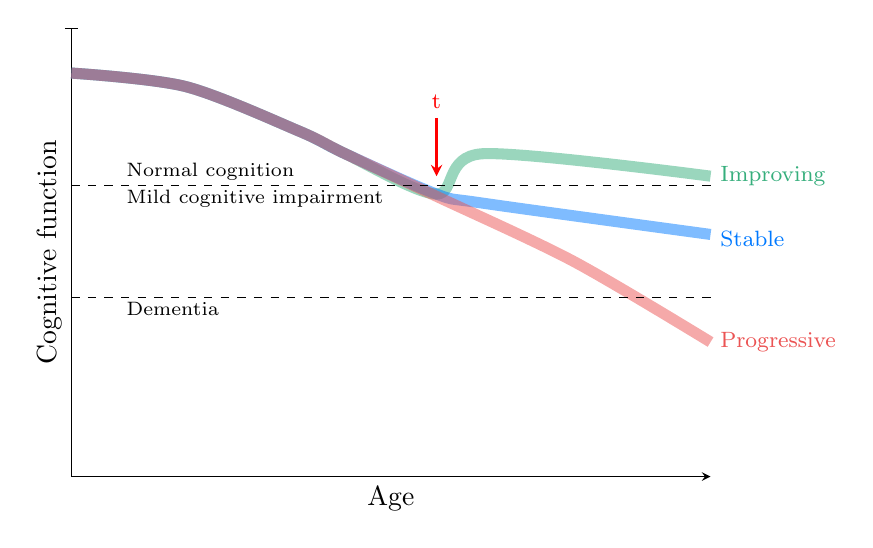
\begin{tikzpicture}
			\begin{axis}[
				height=0.6\textwidth,
				width=0.8\textwidth,
				xlabel={Age},
				ylabel={Cognitive function},
				ticks=none,
				axis x line=bottom,
				axis y line=left,
				y axis line style={-|},
				xmin=0,
				xmax=1.4,
				ymin=0,
				ymax=1,
				clip=false
			]
			\addplot[draw=healthy-default, smooth, line width=4pt, opacity=0.5] coordinates {
				(0, 0.9)
				(0.25, 0.87)
				(0.5, 0.77)
				(0.6, 0.72)
				(0.8, 0.63)
				(0.9, 0.72)
				(1.4, 0.67)
			};
			\addplot[draw=controls-default, smooth, line width=4pt, opacity=0.5] coordinates {
				(0, 0.9)
				(0.25, 0.87)
				(0.5, 0.77)
				(0.6, 0.72)
				(0.8, 0.63)
				(0.9, 0.61)
				(1.4, 0.54)
			};
			\addplot[draw=cases-default, smooth, line width=4pt, opacity=0.5] coordinates {
				(0, 0.9)
				(0.25, 0.87)
				(0.5, 0.77)
				(0.6, 0.72)
				(0.8, 0.625)
				(1.1, 0.48)
				(1.4, 0.3)
			};
			\addplot[dashed] coordinates {
				(0, 0.65)
				(1.4, 0.65)
			};
			\addplot[dashed] coordinates {
				(0, 0.4)
				(1.4, 0.4)
			};
			\node[anchor=south west] at (axis cs: 0.1, 0.64) {\scriptsize{Normal cognition}};
			\node[anchor=north west] at (axis cs: 0.1, 0.66) {\scriptsize{Mild cognitive impairment}};
			\node[anchor=north west] at (axis cs: 0.1, 0.41) {\scriptsize{Dementia}};
			\node[anchor=west] at (axis cs: 1.4, 0.67) {\textcolor{healthy-default}{\footnotesize{Improving}}};
			\node[anchor=west] at (axis cs: 1.4, 0.53) {\textcolor{controls-default}{\footnotesize{Stable}}};
			\node[anchor=west] at (axis cs: 1.4, 0.3) {\textcolor{cases-default}{\footnotesize{Progressive}}};
			\draw[-stealth, red, thick] (axis cs: 0.8, 0.8) -- (axis cs: 0.8, 0.67);
			\node[anchor=south] at (axis cs: 0.8, 0.8) {\textcolor{red}{\footnotesize{t}}};
			\end{axis}
		\end{tikzpicture}
		\vfill
	\end{frame}

	\begin{frame}{Paper 3: Explainable AI and dementia} % Prognosis
		\centering
		\vfill
		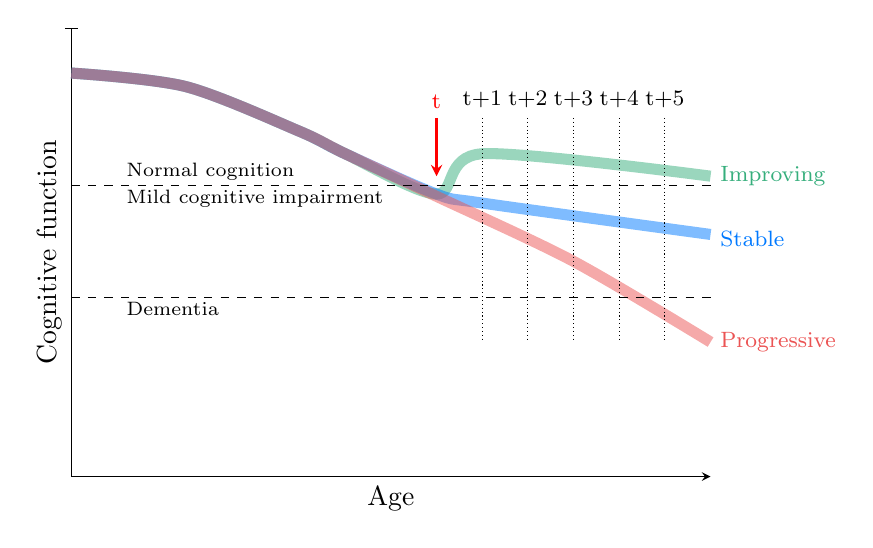
\begin{tikzpicture}
			\begin{axis}[
				height=0.6\textwidth,
				width=0.8\textwidth,
				xlabel={Age},
				ylabel={Cognitive function},
				ticks=none,
				axis x line=bottom,
				axis y line=left,
				y axis line style={-|},
				xmin=0,
				xmax=1.4,
				ymin=0,
				ymax=1,
				clip=false
			]
			\addplot[draw=healthy-default, smooth, line width=4pt, opacity=0.5] coordinates {
				(0, 0.9)
				(0.25, 0.87)
				(0.5, 0.77)
				(0.6, 0.72)
				(0.8, 0.63)
				(0.9, 0.72)
				(1.4, 0.67)
			};
			\addplot[draw=controls-default, smooth, line width=4pt, opacity=0.5] coordinates {
				(0, 0.9)
				(0.25, 0.87)
				(0.5, 0.77)
				(0.6, 0.72)
				(0.8, 0.63)
				(0.9, 0.61)
				(1.4, 0.54)
			};
			\addplot[draw=cases-default, smooth, line width=4pt, opacity=0.5] coordinates {
				(0, 0.9)
				(0.25, 0.87)
				(0.5, 0.77)
				(0.6, 0.72)
				(0.8, 0.625)
				(1.1, 0.48)
				(1.4, 0.3)
			};
			\addplot[dashed] coordinates {
				(0, 0.65)
				(1.4, 0.65)
			};
			\addplot[dashed] coordinates {
				(0, 0.4)
				(1.4, 0.4)
			};
			\node[anchor=south west] at (axis cs: 0.1, 0.64) {\scriptsize{Normal cognition}};
			\node[anchor=north west] at (axis cs: 0.1, 0.66) {\scriptsize{Mild cognitive impairment}};
			\node[anchor=north west] at (axis cs: 0.1, 0.41) {\scriptsize{Dementia}};
			\node[anchor=west] at (axis cs: 1.4, 0.67) {\textcolor{healthy-default}{\footnotesize{Improving}}};
			\node[anchor=west] at (axis cs: 1.4, 0.53) {\textcolor{controls-default}{\footnotesize{Stable}}};
			\node[anchor=west] at (axis cs: 1.4, 0.3) {\textcolor{cases-default}{\footnotesize{Progressive}}};
			\draw[-stealth, red, thick] (axis cs: 0.8, 0.8) -- (axis cs: 0.8, 0.67);
			\node[anchor=south] at (axis cs: 0.8, 0.8) {\textcolor{red}{\footnotesize{t}}};
			\draw[densely dotted] (axis cs: 0.9, 0.8) -- (axis cs: 0.9, 0.3);
			\draw[densely dotted] (axis cs: 1, 0.8) -- (axis cs: 1, 0.3);
			\draw[densely dotted] (axis cs: 1.1, 0.8) -- (axis cs: 1.1, 0.3);
			\draw[densely dotted] (axis cs: 1.2, 0.8) -- (axis cs: 1.2, 0.3);
			\draw[densely dotted] (axis cs: 1.3, 0.8) -- (axis cs: 1.3, 0.3);
			\node[anchor=south] at (axis cs: 0.9, 0.8) {\footnotesize{t+1}};
			\node[anchor=south] at (axis cs: 1, 0.8) {\footnotesize{t+2}};
			\node[anchor=south] at (axis cs: 1.1, 0.8) {\footnotesize{t+3}};
			\node[anchor=south] at (axis cs: 1.2, 0.8) {\footnotesize{t+4}};
			\node[anchor=south] at (axis cs: 1.3, 0.8) {\footnotesize{t+5}};
			\end{axis}
		\end{tikzpicture}
		\vfill
	\end{frame}

	\begin{frame}{Paper 3: Explainable AI and dementia} % Prognosis
		\centering
		\vfill
		\newsavebox{\resultsboxtwo}
			\sbox{\resultsboxtwo}{%
			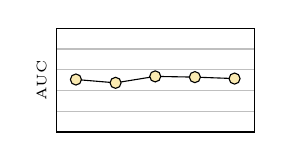
\begin{tikzpicture}
				\begin{axis}[
					height=2.9cm,
					width=4.1cm,
					xmajorticks=false,
					xmin=0.5,
					xmax=5.5,
					ymin=0,
					ymax=1,
					ylabel=\tiny{AUC},
					ymajorticks=false,
					ymajorgrids=true
				]
					\addplot[mark=*, draw=black, mark options={fill=baseline}] coordinates {
						(1, 0.506)
						(2, 0.474)
						(3, 0.536)
						(4, 0.529)
						(5, 0.515)
					};
				\end{axis}
			\end{tikzpicture}
		}
		\begin{tikzpicture}
			\begin{axis}[
				height=0.6\textwidth,
				width=0.8\textwidth,
				xlabel={Age},
				ylabel={Cognitive function},
				ticks=none,
				axis x line=bottom,
				axis y line=left,
				y axis line style={-|},
				xmin=0,
				xmax=1.4,
				ymin=0,
				ymax=1,
				clip=false
			]
			\addplot[draw=healthy-default, smooth, line width=4pt, opacity=0.5] coordinates {
				(0, 0.9)
				(0.25, 0.87)
				(0.5, 0.77)
				(0.6, 0.72)
				(0.8, 0.63)
				(0.9, 0.72)
				(1.4, 0.67)
			};
			\addplot[draw=controls-default, smooth, line width=4pt, opacity=0.5] coordinates {
				(0, 0.9)
				(0.25, 0.87)
				(0.5, 0.77)
				(0.6, 0.72)
				(0.8, 0.63)
				(0.9, 0.61)
				(1.4, 0.54)
			};
			\addplot[draw=cases-default, smooth, line width=4pt, opacity=0.5] coordinates {
				(0, 0.9)
				(0.25, 0.87)
				(0.5, 0.77)
				(0.6, 0.72)
				(0.8, 0.625)
				(1.1, 0.48)
				(1.4, 0.3)
			};
			\addplot[dashed] coordinates {
				(0, 0.65)
				(1.4, 0.65)
			};
			\addplot[dashed] coordinates {
				(0, 0.4)
				(1.4, 0.4)
			};
			\node[anchor=south west] at (axis cs: 0.1, 0.64) {\scriptsize{Normal cognition}};
			\node[anchor=north west] at (axis cs: 0.1, 0.66) {\scriptsize{Mild cognitive impairment}};
			\node[anchor=north west] at (axis cs: 0.1, 0.41) {\scriptsize{Dementia}};
			\node[anchor=west] at (axis cs: 1.4, 0.67) {\textcolor{healthy-default}{\footnotesize{Improving}}};
			\node[anchor=west] at (axis cs: 1.4, 0.53) {\textcolor{controls-default}{\footnotesize{Stable}}};
			\node[anchor=west] at (axis cs: 1.4, 0.3) {\textcolor{cases-default}{\footnotesize{Progressive}}};
			\draw[-stealth, red, thick] (axis cs: 0.8, 0.8) -- (axis cs: 0.8, 0.67);
			\node[anchor=south] at (axis cs: 0.8, 0.8) {\textcolor{red}{\footnotesize{t}}};
			\draw[densely dotted] (axis cs: 0.9, 0.8) -- (axis cs: 0.9, 0.3);
			\draw[densely dotted] (axis cs: 1, 0.8) -- (axis cs: 1, 0.3);
			\draw[densely dotted] (axis cs: 1.1, 0.8) -- (axis cs: 1.1, 0.3);
			\draw[densely dotted] (axis cs: 1.2, 0.8) -- (axis cs: 1.2, 0.3);
			\draw[densely dotted] (axis cs: 1.3, 0.8) -- (axis cs: 1.3, 0.3);
			\node[anchor=south] at (axis cs: 0.9, 0.8) {\footnotesize{t+1}};
			\node[anchor=south] at (axis cs: 1, 0.8) {\footnotesize{t+2}};
			\node[anchor=south] at (axis cs: 1.1, 0.8) {\footnotesize{t+3}};
			\node[anchor=south] at (axis cs: 1.2, 0.8) {\footnotesize{t+4}};
			\node[anchor=south] at (axis cs: 1.3, 0.8) {\footnotesize{t+5}};
			\node[] at (axis cs: 1.0755, 0.155) {
				\usebox{\resultsboxtwo}
			};
			\node[anchor=west] at (axis cs: 1.34, 0.158) {\footnotesize{0.51}};
			\end{axis}
		\end{tikzpicture}
		\vfill
	\end{frame}

	\begin{frame}{Paper 3: Explainable AI and dementia} % Prognosis
		\centering
		\vfill
		\newsavebox{\resultsboxone}
			\sbox{\resultsboxone}{%
			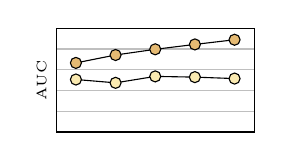
\begin{tikzpicture}
				\begin{axis}[
					height=2.9cm,
					width=4.1cm,
					xmajorticks=false,
					xmin=0.5,
					xmax=5.5,
					ymin=0,
					ymax=1,
					ylabel=\tiny{AUC},
					ymajorticks=false,
					ymajorgrids=true
				]
					\addplot[mark=*, draw=black, mark options={fill=baseline}] coordinates {
						(1, 0.506)
						(2, 0.474)
						(3, 0.536)
						(4, 0.529)
						(5, 0.515)
					};
					\addplot[mark=*, draw=black, mark options={fill=preds}] coordinates {
						(1, 0.666)
						(2, 0.742)
						(3, 0.797)
						(4, 0.844)
						(5, 0.889)
					};
				\end{axis}
			\end{tikzpicture}
		}
		\begin{tikzpicture}
			\begin{axis}[
				height=0.6\textwidth,
				width=0.8\textwidth,
				xlabel={Age},
				ylabel={Cognitive function},
				ticks=none,
				axis x line=bottom,
				axis y line=left,
				y axis line style={-|},
				xmin=0,
				xmax=1.4,
				ymin=0,
				ymax=1,
				clip=false
			]
			\addplot[draw=healthy-default, smooth, line width=4pt, opacity=0.5] coordinates {
				(0, 0.9)
				(0.25, 0.87)
				(0.5, 0.77)
				(0.6, 0.72)
				(0.8, 0.63)
				(0.9, 0.72)
				(1.4, 0.67)
			};
			\addplot[draw=controls-default, smooth, line width=4pt, opacity=0.5] coordinates {
				(0, 0.9)
				(0.25, 0.87)
				(0.5, 0.77)
				(0.6, 0.72)
				(0.8, 0.63)
				(0.9, 0.61)
				(1.4, 0.54)
			};
			\addplot[draw=cases-default, smooth, line width=4pt, opacity=0.5] coordinates {
				(0, 0.9)
				(0.25, 0.87)
				(0.5, 0.77)
				(0.6, 0.72)
				(0.8, 0.625)
				(1.1, 0.48)
				(1.4, 0.3)
			};
			\addplot[dashed] coordinates {
				(0, 0.65)
				(1.4, 0.65)
			};
			\addplot[dashed] coordinates {
				(0, 0.4)
				(1.4, 0.4)
			};
			\node[anchor=south west] at (axis cs: 0.1, 0.64) {\scriptsize{Normal cognition}};
			\node[anchor=north west] at (axis cs: 0.1, 0.66) {\scriptsize{Mild cognitive impairment}};
			\node[anchor=north west] at (axis cs: 0.1, 0.41) {\scriptsize{Dementia}};
			\node[anchor=west] at (axis cs: 1.4, 0.67) {\textcolor{healthy-default}{\footnotesize{Improving}}};
			\node[anchor=west] at (axis cs: 1.4, 0.53) {\textcolor{controls-default}{\footnotesize{Stable}}};
			\node[anchor=west] at (axis cs: 1.4, 0.3) {\textcolor{cases-default}{\footnotesize{Progressive}}};
			\draw[-stealth, red, thick] (axis cs: 0.8, 0.8) -- (axis cs: 0.8, 0.67);
			\node[anchor=south] at (axis cs: 0.8, 0.8) {\textcolor{red}{\footnotesize{t}}};
			\draw[densely dotted] (axis cs: 0.9, 0.8) -- (axis cs: 0.9, 0.3);
			\draw[densely dotted] (axis cs: 1, 0.8) -- (axis cs: 1, 0.3);
			\draw[densely dotted] (axis cs: 1.1, 0.8) -- (axis cs: 1.1, 0.3);
			\draw[densely dotted] (axis cs: 1.2, 0.8) -- (axis cs: 1.2, 0.3);
			\draw[densely dotted] (axis cs: 1.3, 0.8) -- (axis cs: 1.3, 0.3);
			\node[anchor=south] at (axis cs: 0.9, 0.8) {\footnotesize{t+1}};
			\node[anchor=south] at (axis cs: 1, 0.8) {\footnotesize{t+2}};
			\node[anchor=south] at (axis cs: 1.1, 0.8) {\footnotesize{t+3}};
			\node[anchor=south] at (axis cs: 1.2, 0.8) {\footnotesize{t+4}};
			\node[anchor=south] at (axis cs: 1.3, 0.8) {\footnotesize{t+5}};
			\node[] at (axis cs: 1.0755, 0.155) {
				\usebox{\resultsboxone}
			};
			\node[anchor=west] at (axis cs: 1.34, 0.261) {\footnotesize{0.88}};
			\end{axis}
		\end{tikzpicture}
		\vfill
	\end{frame}

	\begin{frame}{Paper 3: Explainable AI and dementia} % Prognosis
		\centering
		\vfill
		\newsavebox{\resultsbox}
			\sbox{\resultsbox}{%
			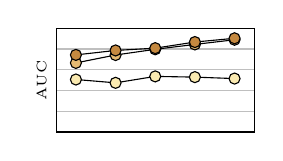
\begin{tikzpicture}
				\begin{axis}[
					height=2.9cm,
					width=4.1cm,
					xmajorticks=false,
					xmin=0.5,
					xmax=5.5,
					ymin=0,
					ymax=1,
					ylabel=\tiny{AUC},
					ymajorticks=false,
					ymajorgrids=true
				]
					\addplot[mark=*, draw=black, mark options={fill=baseline}] coordinates {
						(1, 0.506)
						(2, 0.474)
						(3, 0.536)
						(4, 0.529)
						(5, 0.515)
					};
					\addplot[mark=*, draw=black, mark options={fill=preds}] coordinates {
						(1, 0.666)
						(2, 0.742)
						(3, 0.797)
						(4, 0.844)
						(5, 0.889)
					};
					\addplot[mark=*, draw=black, mark options={fill=maps}] coordinates {
						(1, 0.743)
						(2, 0.786)
						(3, 0.808)
						(4, 0.867)
						(5, 0.903)
					};
				\end{axis}
			\end{tikzpicture}
		}
		\begin{tikzpicture}
			\begin{axis}[
				height=0.6\textwidth,
				width=0.8\textwidth,
				xlabel={Age},
				ylabel={Cognitive function},
				ticks=none,
				axis x line=bottom,
				axis y line=left,
				y axis line style={-|},
				xmin=0,
				xmax=1.4,
				ymin=0,
				ymax=1,
				clip=false
			]
			\addplot[draw=healthy-default, smooth, line width=4pt, opacity=0.5] coordinates {
				(0, 0.9)
				(0.25, 0.87)
				(0.5, 0.77)
				(0.6, 0.72)
				(0.8, 0.63)
				(0.9, 0.72)
				(1.4, 0.67)
			};
			\addplot[draw=controls-default, smooth, line width=4pt, opacity=0.5] coordinates {
				(0, 0.9)
				(0.25, 0.87)
				(0.5, 0.77)
				(0.6, 0.72)
				(0.8, 0.63)
				(0.9, 0.61)
				(1.4, 0.54)
			};
			\addplot[draw=cases-default, smooth, line width=4pt, opacity=0.5] coordinates {
				(0, 0.9)
				(0.25, 0.87)
				(0.5, 0.77)
				(0.6, 0.72)
				(0.8, 0.625)
				(1.1, 0.48)
				(1.4, 0.3)
			};
			\addplot[dashed] coordinates {
				(0, 0.65)
				(1.4, 0.65)
			};
			\addplot[dashed] coordinates {
				(0, 0.4)
				(1.4, 0.4)
			};
			\node[anchor=south west] at (axis cs: 0.1, 0.64) {\scriptsize{Normal cognition}};
			\node[anchor=north west] at (axis cs: 0.1, 0.66) {\scriptsize{Mild cognitive impairment}};
			\node[anchor=north west] at (axis cs: 0.1, 0.41) {\scriptsize{Dementia}};
			\node[anchor=west] at (axis cs: 1.4, 0.67) {\textcolor{healthy-default}{\footnotesize{Improving}}};
			\node[anchor=west] at (axis cs: 1.4, 0.53) {\textcolor{controls-default}{\footnotesize{Stable}}};
			\node[anchor=west] at (axis cs: 1.4, 0.3) {\textcolor{cases-default}{\footnotesize{Progressive}}};
			\draw[-stealth, red, thick] (axis cs: 0.8, 0.8) -- (axis cs: 0.8, 0.67);
			\node[anchor=south] at (axis cs: 0.8, 0.8) {\textcolor{red}{\footnotesize{t}}};
			\draw[densely dotted] (axis cs: 0.9, 0.8) -- (axis cs: 0.9, 0.3);
			\draw[densely dotted] (axis cs: 1, 0.8) -- (axis cs: 1, 0.3);
			\draw[densely dotted] (axis cs: 1.1, 0.8) -- (axis cs: 1.1, 0.3);
			\draw[densely dotted] (axis cs: 1.2, 0.8) -- (axis cs: 1.2, 0.3);
			\draw[densely dotted] (axis cs: 1.3, 0.8) -- (axis cs: 1.3, 0.3);
			\node[anchor=south] at (axis cs: 0.9, 0.8) {\footnotesize{t+1}};
			\node[anchor=south] at (axis cs: 1, 0.8) {\footnotesize{t+2}};
			\node[anchor=south] at (axis cs: 1.1, 0.8) {\footnotesize{t+3}};
			\node[anchor=south] at (axis cs: 1.2, 0.8) {\footnotesize{t+4}};
			\node[anchor=south] at (axis cs: 1.3, 0.8) {\footnotesize{t+5}};
			\node[] at (axis cs: 1.0755, 0.155) {
				\usebox{\resultsbox}
			};
			\node[anchor=west] at (axis cs: 1.34, 0.262) {\footnotesize{0.90}};
			\end{axis}
		\end{tikzpicture}
		\vfill
	\end{frame}

	\begin{frame}{Paper 3: Explainable AI and dementia} % Correlations
		\newcommand{\mriwidth}{2.2cm}
        \newcommand{\gap}{0.00cm}

        \newcommand{\correlationplot}[4]{
            \begin{tikzpicture}
                \begin{axis}[
                    height=1.71 * \mriwidth,
                    width=1.71 * \mriwidth,
                    xmajorticks=false,
                    ylabel=####3,
                    ytick={0, 2, 4, 6, 8},
                    yticklabels=####2,
                    xmin=-1,
                    xmax=17,
                    ymin=0,
                    ymax=9,
                    every tick label/.append style={font=\tiny},
                    ytick pos=left,
                    scatter/classes={
                        ADNI_EF={color0, draw=black},
                        ADNI_MEM={color1, draw=black},
                        CDCARE={color2, draw=black},
                        CDCOMMUN={color3, draw=black},
                        CDGLOBAL={color4, draw=black},
                        CDHOME={color5, draw=black},
                        CDJUDGE={color6, draw=black},
                        CDMEMORY={color7, draw=black},
                        CDORIENT={color8, draw=black},
                        FAQTOTAL={color9, draw=black},
                        GDTOTAL={color10, draw=black},
                        MMSCORE={color11, draw=black},
                        NPISCORE={color12, draw=black},
                        PHC_EXF={color13, draw=black},
                        PHC_LAN={color14, draw=black},
                        PHC_MEM={color15, draw=black},
                        PHC_VSP={color16, draw=black}
                    },
                    y label style={at={(-0.1,0.5)}},
                    ymajorgrids=true,
                    ytick style={draw=none},
                    clip=false,
                    grid style={draw=gray!20},
                    axis line style={draw=gray!70}
                ]
                    \addplot[
                        only marks,
                        scatter,
                        scatter src=explicit symbolic
                    ] table [
                        col sep=comma,
                        x=index,
                        y=component_####1,
                        meta=symptom
                    ] {data/correlations.csv};
                    \addplot[dashed,red, thick] coordinates {
                        (-1, 2.76)
                        (17, 2.76)
                    };
                    ####4
                \end{axis}
            \end{tikzpicture}
        }

        \newsavebox{\firstcorrelations}
        \sbox{\firstcorrelations}{%
            \correlationplot{0}{{0, 2, 4, 6, 8}}{\scriptsize{$-log_{10}(p)$}}{
                \node[] at (axis cs: 14, 6.09) {\tiny{PHC\_LAN}};
            }
        }
        \newsavebox{\secondcorrelations}
        \sbox{\secondcorrelations}{%
            \correlationplot{1}{{,,}}{{}}{
                \node[] at (axis cs: 9, 3.64) {\tiny{FAQTOTAL}};
            }
        }
        \newsavebox{\thirdcorrelations}
        \sbox{\thirdcorrelations}{%
            \correlationplot{2}{{,,}}{{}}{
                \node[] at (axis cs: 0, 6.34) {\tiny{ADNI\_EF}};
                \node[] at (axis cs: 13, 7.85) {\tiny{PHC\_EXF}};
            }
        }
        \newsavebox{\fourthcorrelations}
        \sbox{\fourthcorrelations}{%
            \correlationplot{3}{{,,}}{{}}{
                \node[] at (axis cs: 0, 8.92) {\tiny{ADNI\_EF}};
                \node[] at (axis cs: 13, 8.65) {\tiny{PHC\_EXF}};
                \node[] at (axis cs: 14, 5.84) {\tiny{PHC\_LAN}};
                \node[] at (axis cs: 6, 5.08) {\tiny{CDJUDGE}};
                \node[] at (axis cs: 11, 3.89) {\tiny{MMSCORE}};
            }
        }

        \begin{tikzpicture}
            \node[] (first) at (0, 0) {
                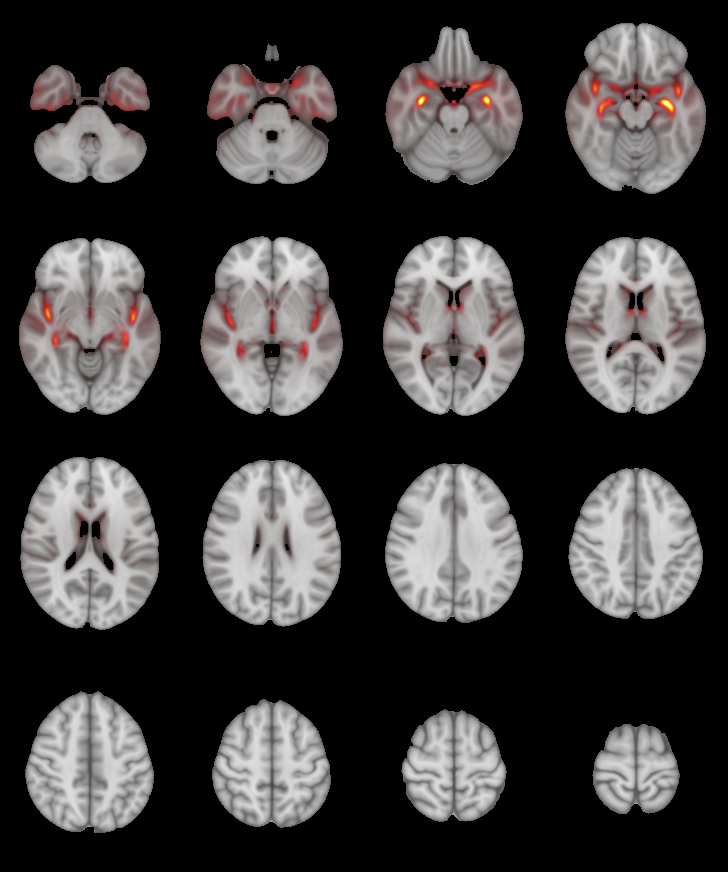
\includegraphics[
                    width=\mriwidth,
                    clip=true,
                    trim = 192mm 232mm 0mm 0mm
                ]{data/components/component_0.png}
            };
            \node[anchor=north west] (first-correlation) at ($ (first.south west) + (-0.73, 0.1) $) {
                \usebox{\firstcorrelations}
            };

            \node[anchor=west] (second) at ($ (first.east) + (\gap, 0) $) {
                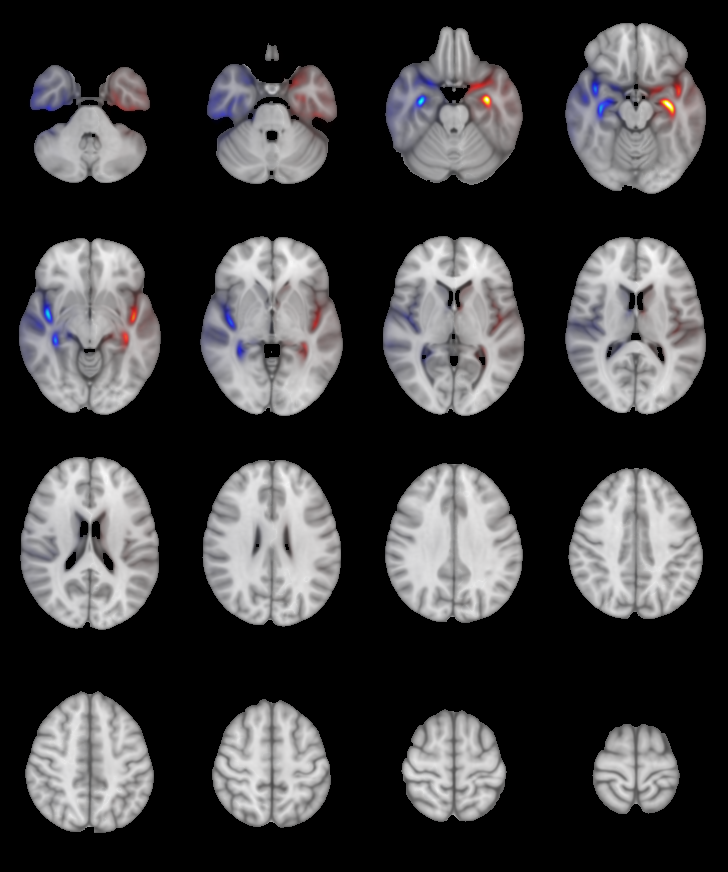
\includegraphics[
                    width=\mriwidth,
                    clip=true,
                    trim = 192mm 232mm 0mm 0mm
                ]{data/components/component_1.png}
            };
            \node[anchor=north west] (second-correlation) at ($ (first-correlation.north east) - (0.56, 0) $) {
                \usebox{\secondcorrelations}
            };

            \node[anchor=west] (third) at ($ (second.east) + (\gap, 0) $) {
                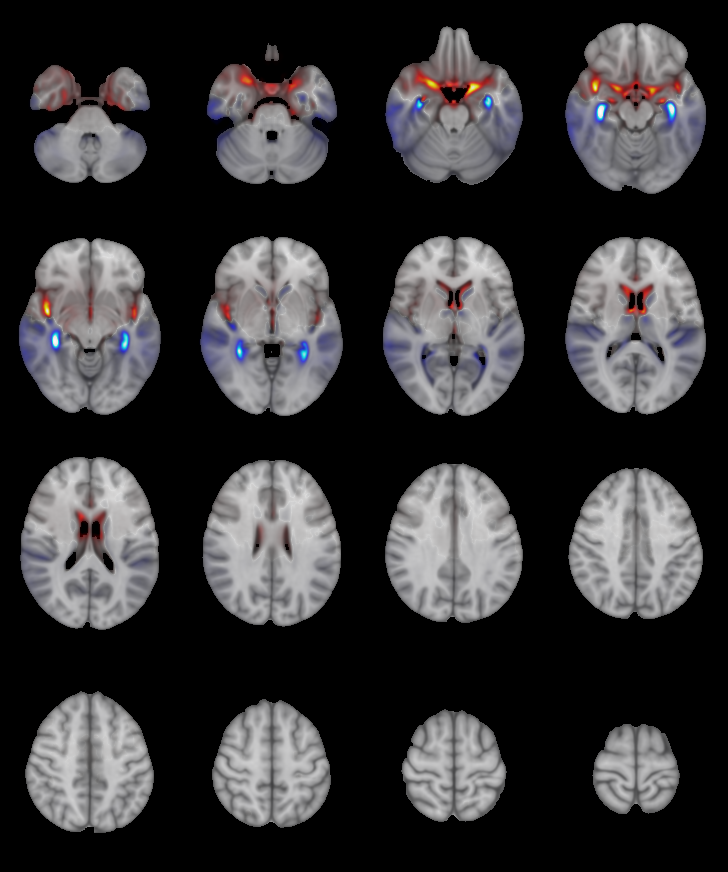
\includegraphics[
                    width=\mriwidth,
                    clip=true,
                    trim = 192mm 232mm 0mm 0mm
                ]{data/components/component_2.png}
            };
            \node[anchor=north west] (third-correlation) at ($ (second-correlation.north east) - (0.56, 0) $) {
                \usebox{\thirdcorrelations}
            };

            \node[anchor=west] (fourth) at ($ (third.east) + (\gap, 0) $) {
                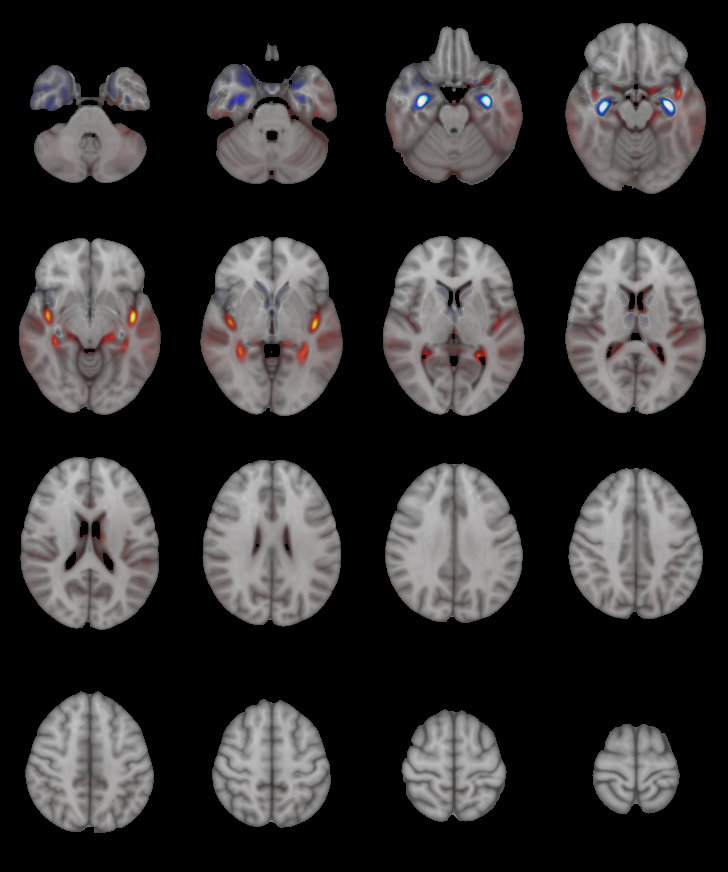
\includegraphics[
                    width=\mriwidth,
                    clip=true,
                    trim = 192mm 232mm 0mm 0mm
                ]{data/components/component_3.png}
            };
            \node[anchor=north west] (fourth-correlation) at ($ (third-correlation.north east) - (0.56, -0.16) $) {
                \usebox{\fourthcorrelations}
            };
        \end{tikzpicture}
	\end{frame}

	\begin{frame}{Paper 4: Explainable brain age}
		\centering
		\vfill
		\begin{tikzpicture}
			\node[inner sep=1pt, fill=white, draw=black] {
				
\includegraphics[width=8cm]{data/paper4.png}
			};
		\end{tikzpicture}
		\vfill
	\end{frame}

	\begin{frame}{Paper 4: Explainable brain age}
		\begin{figure}
			\scalebox{.4}{
			\begin{minipage}[b]{0.78\textwidth}
				\hspace{1.69cm}\begin{subfigure}[b]{\textwidth}

					\begin{tikzpicture}
						\pgfplotstableread[col sep=comma]{/Users/esten/phd/papers/2023-explainable-brain-age/data/full_data_distributions.csv}\data
						\begin{axis}[
							width=0.97\textwidth,
							height=0.85\textwidth,
							xmin=0,
							xmax=100,
							ytick=\empty,
							axis x line=middle,
							axis y line=none,
							xtick={10,20,30,40,50,60,70,80},
							x axis line style={|-stealth},
						]
							\addplot[
								name path=zero,
							] coordinates {(0,0) (100,0)};
							\addplot [
								draw=none,
								line width=0pt,
								name path={female_ds002424},
							] table [
								x=age,
								y expr=1 * \thisrow{female_ds002424}
							]{\data};
							\addplot [
								draw=none,
								line width=0pt,
								name path={female_HBN},
							] table [
								x=age,
								y expr=1 * \thisrow{female_HBN}
							]{\data};
							\addplot [
								draw=none,
								line width=0pt,
								name path={female_ABCD},
							] table [
								x=age,
								y expr=1 * \thisrow{female_ABCD}
							]{\data};
							\addplot [
								draw=none,
								line width=0pt,
								name path={female_QTAB},
							] table [
								x=age,
								y expr=1 * \thisrow{female_QTAB}
							]{\data};
							\addplot [
								draw=none,
								line width=0pt,
								name path={female_PING},
							] table [
								x=age,
								y expr=1 * \thisrow{female_PING}
							]{\data};
							\addplot [
								draw=none,
								line width=0pt,
								name path={female_ADHD200},
							] table [
								x=age,
								y expr=1 * \thisrow{female_ADHD200}
							]{\data};
							\addplot [
								draw=none,
								line width=0pt,
								name path={female_PNC},
							] table [
								x=age,
								y expr=1 * \thisrow{female_PNC}
							]{\data};
							\addplot [
								draw=none,
								line width=0pt,
								name path={female_ABIDE II},
							] table [
								x=age,
								y expr=1 * \thisrow{female_ABIDE II}
							]{\data};
							\addplot [
								draw=none,
								line width=0pt,
								name path={female_ds000119},
							] table [
								x=age,
								y expr=1 * \thisrow{female_ds000119}
							]{\data};
							\addplot [
								draw=none,
								line width=0pt,
								name path={female_ABIDE I},
							] table [
								x=age,
								y expr=1 * \thisrow{female_ABIDE I}
							]{\data};
							\addplot [
								draw=none,
								line width=0pt,
								name path={female_BRAINMINT},
							] table [
								x=age,
								y expr=1 * \thisrow{female_BRAINMINT}
							]{\data};
							\addplot [
								draw=none,
								line width=0pt,
								name path={female_SLIM},
							] table [
								x=age,
								y expr=1 * \thisrow{female_SLIM}
							]{\data};
							\addplot [
								draw=none,
								line width=0pt,
								name path={female_QTIM},
							] table [
								x=age,
								y expr=1 * \thisrow{female_QTIM}
							]{\data};
							\addplot [
								draw=none,
								line width=0pt,
								name path={female_Beijing},
							] table [
								x=age,
								y expr=1 * \thisrow{female_Beijing}
							]{\data};
							\addplot [
								draw=none,
								line width=0pt,
								name path={female_AOMIC-PIOP2},
							] table [
								x=age,
								y expr=1 * \thisrow{female_AOMIC-PIOP2}
							]{\data};
							\addplot [
								draw=none,
								line width=0pt,
								name path={female_ds000202},
							] table [
								x=age,
								y expr=1 * \thisrow{female_ds000202}
							]{\data};
							\addplot [
								draw=none,
								line width=0pt,
								name path={female_AOMIC-PIOP1},
							] table [
								x=age,
								y expr=1 * \thisrow{female_AOMIC-PIOP1}
							]{\data};
							\addplot [
								draw=none,
								line width=0pt,
								name path={female_AOMIC-ID1000},
							] table [
								x=age,
								y expr=1 * \thisrow{female_AOMIC-ID1000}
							]{\data};
							\addplot [
								draw=none,
								line width=0pt,
								name path={female_CoRR},
							] table [
								x=age,
								y expr=1 * \thisrow{female_CoRR}
							]{\data};
							\addplot [
								draw=none,
								line width=0pt,
								name path={female_HCP},
							] table [
								x=age,
								y expr=1 * \thisrow{female_HCP}
							]{\data};
							\addplot [
								draw=none,
								line width=0pt,
								name path={female_FCON1000},
							] table [
								x=age,
								y expr=1 * \thisrow{female_FCON1000}
							]{\data};
							\addplot [
								draw=none,
								line width=0pt,
								name path={female_ds000171},
							] table [
								x=age,
								y expr=1 * \thisrow{female_ds000171}
							]{\data};
							\addplot [
								draw=none,
								line width=0pt,
								name path={female_TOP},
							] table [
								x=age,
								y expr=1 * \thisrow{female_TOP}
							]{\data};
							\addplot [
								draw=none,
								line width=0pt,
								name path={female_SCZ-Z},
							] table [
								x=age,
								y expr=1 * \thisrow{female_SCZ-Z}
							]{\data};
							\addplot [
								draw=none,
								line width=0pt,
								name path={female_NIMH},
							] table [
								x=age,
								y expr=1 * \thisrow{female_NIMH}
							]{\data};
							\addplot [
								draw=none,
								line width=0pt,
								name path={female_NKI-RS},
							] table [
								x=age,
								y expr=1 * \thisrow{female_NKI-RS}
							]{\data};
							\addplot [
								draw=none,
								line width=0pt,
								name path={female_MPI-LEMON},
							] table [
								x=age,
								y expr=1 * \thisrow{female_MPI-LEMON}
							]{\data};
							\addplot [
								draw=none,
								line width=0pt,
								name path={female_ds003592},
							] table [
								x=age,
								y expr=1 * \thisrow{female_ds003592}
							]{\data};
							\addplot [
								draw=none,
								line width=0pt,
								name path={female_ds004302},
							] table [
								x=age,
								y expr=1 * \thisrow{female_ds004302}
							]{\data};
							\addplot [
								draw=none,
								line width=0pt,
								name path={female_ds000222},
							] table [
								x=age,
								y expr=1 * \thisrow{female_ds000222}
							]{\data};
							\addplot [
								draw=none,
								line width=0pt,
								name path={female_SALD},
							] table [
								x=age,
								y expr=1 * \thisrow{female_SALD}
							]{\data};
							\addplot [
								draw=none,
								line width=0pt,
								name path={female_IXI},
							] table [
								x=age,
								y expr=1 * \thisrow{female_IXI}
							]{\data};
							\addplot [
								draw=none,
								line width=0pt,
								name path={female_DLBS},
							] table [
								x=age,
								y expr=1 * \thisrow{female_DLBS}
							]{\data};
							\addplot [
								draw=none,
								line width=0pt,
								name path={female_Cam-CAN},
							] table [
								x=age,
								y expr=1 * \thisrow{female_Cam-CAN}
							]{\data};
							\addplot [
								draw=none,
								line width=0pt,
								name path={female_StrokeMRI},
							] table [
								x=age,
								y expr=1 * \thisrow{female_StrokeMRI}
							]{\data};
							\addplot [
								draw=none,
								line width=0pt,
								name path={female_PPMI},
							] table [
								x=age,
								y expr=1 * \thisrow{female_PPMI}
							]{\data};
							\addplot [
								draw=none,
								line width=0pt,
								name path={female_UKBB},
							] table [
								x=age,
								y expr=1 * \thisrow{female_UKBB}
							]{\data};
							\addplot [
								draw=none,
								line width=0pt,
								name path={female_Tao-Wu},
							] table [
								x=age,
								y expr=1 * \thisrow{female_Tao-Wu}
							]{\data};
							\addplot [
								draw=none,
								line width=0pt,
								name path={female_ds000245},
							] table [
								x=age,
								y expr=1 * \thisrow{female_ds000245}
							]{\data};
							\addplot [
								draw=none,
								line width=0pt,
								name path={female_OASIS3},
							] table [
								x=age,
								y expr=1 * \thisrow{female_OASIS3}
							]{\data};
							\addplot [
								draw=none,
								line width=0pt,
								name path={female_Demgen},
							] table [
								x=age,
								y expr=1 * \thisrow{female_Demgen}
							]{\data};
							\addplot [
								draw=none,
								line width=0pt,
								name path={female_NEUROCON},
							] table [
								x=age,
								y expr=1 * \thisrow{female_NEUROCON}
							]{\data};
							\addplot [
								draw=none,
								line width=0pt,
								name path={female_MIRIAD},
							] table [
								x=age,
								y expr=1 * \thisrow{female_MIRIAD}
							]{\data};
							\addplot [
								draw=none,
								line width=0pt,
								name path={female_ds004392},
							] table [
								x=age,
								y expr=1 * \thisrow{female_ds004392}
							]{\data};
							\addplot [
								draw=none,
								line width=0pt,
								name path={female_AIBL},
							] table [
								x=age,
								y expr=1 * \thisrow{female_AIBL}
							]{\data};
							\addplot [
								draw=none,
								line width=0pt,
								name path={female_ANM},
							] table [
								x=age,
								y expr=1 * \thisrow{female_ANM}
							]{\data};
							\addplot [
								draw=none,
								line width=0pt,
								name path={female_ADNI},
							] table [
								x=age,
								y expr=1 * \thisrow{female_ADNI}
							]{\data};
							\addplot [
								draw=none,
								line width=0pt,
								name path={male_ds002424},
							] table [
								x=age,
								y expr=-1 * \thisrow{male_ds002424}
							]{\data};
							\addplot [
								draw=none,
								line width=0pt,
								name path={male_HBN},
							] table [
								x=age,
								y expr=-1 * \thisrow{male_HBN}
							]{\data};
							\addplot [
								draw=none,
								line width=0pt,
								name path={male_ABCD},
							] table [
								x=age,
								y expr=-1 * \thisrow{male_ABCD}
							]{\data};
							\addplot [
								draw=none,
								line width=0pt,
								name path={male_QTAB},
							] table [
								x=age,
								y expr=-1 * \thisrow{male_QTAB}
							]{\data};
							\addplot [
								draw=none,
								line width=0pt,
								name path={male_PING},
							] table [
								x=age,
								y expr=-1 * \thisrow{male_PING}
							]{\data};
							\addplot [
								draw=none,
								line width=0pt,
								name path={male_ADHD200},
							] table [
								x=age,
								y expr=-1 * \thisrow{male_ADHD200}
							]{\data};
							\addplot [
								draw=none,
								line width=0pt,
								name path={male_PNC},
							] table [
								x=age,
								y expr=-1 * \thisrow{male_PNC}
							]{\data};
							\addplot [
								draw=none,
								line width=0pt,
								name path={male_ABIDE II},
							] table [
								x=age,
								y expr=-1 * \thisrow{male_ABIDE II}
							]{\data};
							\addplot [
								draw=none,
								line width=0pt,
								name path={male_ds000119},
							] table [
								x=age,
								y expr=-1 * \thisrow{male_ds000119}
							]{\data};
							\addplot [
								draw=none,
								line width=0pt,
								name path={male_ABIDE I},
							] table [
								x=age,
								y expr=-1 * \thisrow{male_ABIDE I}
							]{\data};
							\addplot [
								draw=none,
								line width=0pt,
								name path={male_BRAINMINT},
							] table [
								x=age,
								y expr=-1 * \thisrow{male_BRAINMINT}
							]{\data};
							\addplot [
								draw=none,
								line width=0pt,
								name path={male_SLIM},
							] table [
								x=age,
								y expr=-1 * \thisrow{male_SLIM}
							]{\data};
							\addplot [
								draw=none,
								line width=0pt,
								name path={male_QTIM},
							] table [
								x=age,
								y expr=-1 * \thisrow{male_QTIM}
							]{\data};
							\addplot [
								draw=none,
								line width=0pt,
								name path={male_Beijing},
							] table [
								x=age,
								y expr=-1 * \thisrow{male_Beijing}
							]{\data};
							\addplot [
								draw=none,
								line width=0pt,
								name path={male_AOMIC-PIOP2},
							] table [
								x=age,
								y expr=-1 * \thisrow{male_AOMIC-PIOP2}
							]{\data};
							\addplot [
								draw=none,
								line width=0pt,
								name path={male_ds000202},
							] table [
								x=age,
								y expr=-1 * \thisrow{male_ds000202}
							]{\data};
							\addplot [
								draw=none,
								line width=0pt,
								name path={male_AOMIC-PIOP1},
							] table [
								x=age,
								y expr=-1 * \thisrow{male_AOMIC-PIOP1}
							]{\data};
							\addplot [
								draw=none,
								line width=0pt,
								name path={male_AOMIC-ID1000},
							] table [
								x=age,
								y expr=-1 * \thisrow{male_AOMIC-ID1000}
							]{\data};
							\addplot [
								draw=none,
								line width=0pt,
								name path={male_CoRR},
							] table [
								x=age,
								y expr=-1 * \thisrow{male_CoRR}
							]{\data};
							\addplot [
								draw=none,
								line width=0pt,
								name path={male_HCP},
							] table [
								x=age,
								y expr=-1 * \thisrow{male_HCP}
							]{\data};
							\addplot [
								draw=none,
								line width=0pt,
								name path={male_FCON1000},
							] table [
								x=age,
								y expr=-1 * \thisrow{male_FCON1000}
							]{\data};
							\addplot [
								draw=none,
								line width=0pt,
								name path={male_ds000171},
							] table [
								x=age,
								y expr=-1 * \thisrow{male_ds000171}
							]{\data};
							\addplot [
								draw=none,
								line width=0pt,
								name path={male_TOP},
							] table [
								x=age,
								y expr=-1 * \thisrow{male_TOP}
							]{\data};
							\addplot [
								draw=none,
								line width=0pt,
								name path={male_SCZ-Z},
							] table [
								x=age,
								y expr=-1 * \thisrow{male_SCZ-Z}
							]{\data};
							\addplot [
								draw=none,
								line width=0pt,
								name path={male_NIMH},
							] table [
								x=age,
								y expr=-1 * \thisrow{male_NIMH}
							]{\data};
							\addplot [
								draw=none,
								line width=0pt,
								name path={male_NKI-RS},
							] table [
								x=age,
								y expr=-1 * \thisrow{male_NKI-RS}
							]{\data};
							\addplot [
								draw=none,
								line width=0pt,
								name path={male_MPI-LEMON},
							] table [
								x=age,
								y expr=-1 * \thisrow{male_MPI-LEMON}
							]{\data};
							\addplot [
								draw=none,
								line width=0pt,
								name path={male_ds003592},
							] table [
								x=age,
								y expr=-1 * \thisrow{male_ds003592}
							]{\data};
							\addplot [
								draw=none,
								line width=0pt,
								name path={male_ds004302},
							] table [
								x=age,
								y expr=-1 * \thisrow{male_ds004302}
							]{\data};
							\addplot [
								draw=none,
								line width=0pt,
								name path={male_ds000222},
							] table [
								x=age,
								y expr=-1 * \thisrow{male_ds000222}
							]{\data};
							\addplot [
								draw=none,
								line width=0pt,
								name path={male_SALD},
							] table [
								x=age,
								y expr=-1 * \thisrow{male_SALD}
							]{\data};
							\addplot [
								draw=none,
								line width=0pt,
								name path={male_IXI},
							] table [
								x=age,
								y expr=-1 * \thisrow{male_IXI}
							]{\data};
							\addplot [
								draw=none,
								line width=0pt,
								name path={male_DLBS},
							] table [
								x=age,
								y expr=-1 * \thisrow{male_DLBS}
							]{\data};
							\addplot [
								draw=none,
								line width=0pt,
								name path={male_Cam-CAN},
							] table [
								x=age,
								y expr=-1 * \thisrow{male_Cam-CAN}
							]{\data};
							\addplot [
								draw=none,
								line width=0pt,
								name path={male_StrokeMRI},
							] table [
								x=age,
								y expr=-1 * \thisrow{male_StrokeMRI}
							]{\data};
							\addplot [
								draw=none,
								line width=0pt,
								name path={male_PPMI},
							] table [
								x=age,
								y expr=-1 * \thisrow{male_PPMI}
							]{\data};
							\addplot [
								draw=none,
								line width=0pt,
								name path={male_UKBB},
							] table [
								x=age,
								y expr=-1 * \thisrow{male_UKBB}
							]{\data};
							\addplot [
								draw=none,
								line width=0pt,
								name path={male_Tao-Wu},
							] table [
								x=age,
								y expr=-1 * \thisrow{male_Tao-Wu}
							]{\data};
							\addplot [
								draw=none,
								line width=0pt,
								name path={male_ds000245},
							] table [
								x=age,
								y expr=-1 * \thisrow{male_ds000245}
							]{\data};
							\addplot [
								draw=none,
								line width=0pt,
								name path={male_OASIS3},
							] table [
								x=age,
								y expr=-1 * \thisrow{male_OASIS3}
							]{\data};
							\addplot [
								draw=none,
								line width=0pt,
								name path={male_Demgen},
							] table [
								x=age,
								y expr=-1 * \thisrow{male_Demgen}
							]{\data};
							\addplot [
								draw=none,
								line width=0pt,
								name path={male_NEUROCON},
							] table [
								x=age,
								y expr=-1 * \thisrow{male_NEUROCON}
							]{\data};
							\addplot [
								draw=none,
								line width=0pt,
								name path={male_MIRIAD},
							] table [
								x=age,
								y expr=-1 * \thisrow{male_MIRIAD}
							]{\data};
							\addplot [
								draw=none,
								line width=0pt,
								name path={male_ds004392},
							] table [
								x=age,
								y expr=-1 * \thisrow{male_ds004392}
							]{\data};
							\addplot [
								draw=none,
								line width=0pt,
								name path={male_AIBL},
							] table [
								x=age,
								y expr=-1 * \thisrow{male_AIBL}
							]{\data};
							\addplot [
								draw=none,
								line width=0pt,
								name path={male_ANM},
							] table [
								x=age,
								y expr=-1 * \thisrow{male_ANM}
							]{\data};
							\addplot [
								draw=none,
								line width=0pt,
								name path={male_ADNI},
							] table [
								x=age,
								y expr=-1 * \thisrow{male_ADNI}
							]{\data};
							\addplot[
								ds002424!50
							] fill between [
								of=zero and female_ds002424
							];
							\addplot[
								ds002424!50
							] fill between [
								of=zero and male_ds002424
							];
							\addplot[
								HBN!50
							] fill between [
								of=female_ds002424 and female_HBN
							];
							\addplot[
								HBN!50
							] fill between [
								of=male_ds002424 and male_HBN
							];
							\addplot[
								ABCD!50
							] fill between [
								of=female_HBN and female_ABCD
							];
							\addplot[
								ABCD!50
							] fill between [
								of=male_HBN and male_ABCD
							];
							\addplot[
								QTAB!50
							] fill between [
								of=female_ABCD and female_QTAB
							];
							\addplot[
								QTAB!50
							] fill between [
								of=male_ABCD and male_QTAB
							];
							\addplot[
								PING!50
							] fill between [
								of=female_QTAB and female_PING
							];
							\addplot[
								PING!50
							] fill between [
								of=male_QTAB and male_PING
							];
							\addplot[
								ADHD200!50
							] fill between [
								of=female_PING and female_ADHD200
							];
							\addplot[
								ADHD200!50
							] fill between [
								of=male_PING and male_ADHD200
							];
							\addplot[
								PNC!50
							] fill between [
								of=female_ADHD200 and female_PNC
							];
							\addplot[
								PNC!50
							] fill between [
								of=male_ADHD200 and male_PNC
							];
							\addplot[
								ABIDE II!50
							] fill between [
								of=female_PNC and female_ABIDE II
							];
							\addplot[
								ABIDE II!50
							] fill between [
								of=male_PNC and male_ABIDE II
							];
							\addplot[
								ds000119!50
							] fill between [
								of=female_ABIDE II and female_ds000119
							];
							\addplot[
								ds000119!50
							] fill between [
								of=male_ABIDE II and male_ds000119
							];
							\addplot[
								ABIDE I!50
							] fill between [
								of=female_ds000119 and female_ABIDE I
							];
							\addplot[
								ABIDE I!50
							] fill between [
								of=male_ds000119 and male_ABIDE I
							];
							\addplot[
								BRAINMINT!50
							] fill between [
								of=female_ABIDE I and female_BRAINMINT
							];
							\addplot[
								BRAINMINT!50
							] fill between [
								of=male_ABIDE I and male_BRAINMINT
							];
							\addplot[
								SLIM!50
							] fill between [
								of=female_BRAINMINT and female_SLIM
							];
							\addplot[
								SLIM!50
							] fill between [
								of=male_BRAINMINT and male_SLIM
							];
							\addplot[
								QTIM!50
							] fill between [
								of=female_SLIM and female_QTIM
							];
							\addplot[
								QTIM!50
							] fill between [
								of=male_SLIM and male_QTIM
							];
							\addplot[
								Beijing!50
							] fill between [
								of=female_QTIM and female_Beijing
							];
							\addplot[
								Beijing!50
							] fill between [
								of=male_QTIM and male_Beijing
							];
							\addplot[
								AOMIC-PIOP2!50
							] fill between [
								of=female_Beijing and female_AOMIC-PIOP2
							];
							\addplot[
								AOMIC-PIOP2!50
							] fill between [
								of=male_Beijing and male_AOMIC-PIOP2
							];
							\addplot[
								ds000202!50
							] fill between [
								of=female_AOMIC-PIOP2 and female_ds000202
							];
							\addplot[
								ds000202!50
							] fill between [
								of=male_AOMIC-PIOP2 and male_ds000202
							];
							\addplot[
								AOMIC-PIOP1!50
							] fill between [
								of=female_ds000202 and female_AOMIC-PIOP1
							];
							\addplot[
								AOMIC-PIOP1!50
							] fill between [
								of=male_ds000202 and male_AOMIC-PIOP1
							];
							\addplot[
								AOMIC-ID1000!50
							] fill between [
								of=female_AOMIC-PIOP1 and female_AOMIC-ID1000
							];
							\addplot[
								AOMIC-ID1000!50
							] fill between [
								of=male_AOMIC-PIOP1 and male_AOMIC-ID1000
							];
							\addplot[
								CoRR!50
							] fill between [
								of=female_AOMIC-ID1000 and female_CoRR
							];
							\addplot[
								CoRR!50
							] fill between [
								of=male_AOMIC-ID1000 and male_CoRR
							];
							\addplot[
								HCP!50
							] fill between [
								of=female_CoRR and female_HCP
							];
							\addplot[
								HCP!50
							] fill between [
								of=male_CoRR and male_HCP
							];
							\addplot[
								FCON1000!50
							] fill between [
								of=female_HCP and female_FCON1000
							];
							\addplot[
								FCON1000!50
							] fill between [
								of=male_HCP and male_FCON1000
							];
							\addplot[
								ds000171!50
							] fill between [
								of=female_FCON1000 and female_ds000171
							];
							\addplot[
								ds000171!50
							] fill between [
								of=male_FCON1000 and male_ds000171
							];
							\addplot[
								TOP!50
							] fill between [
								of=female_ds000171 and female_TOP
							];
							\addplot[
								TOP!50
							] fill between [
								of=male_ds000171 and male_TOP
							];
							\addplot[
								SCZ-Z!50
							] fill between [
								of=female_TOP and female_SCZ-Z
							];
							\addplot[
								SCZ-Z!50
							] fill between [
								of=male_TOP and male_SCZ-Z
							];
							\addplot[
								NIMH!50
							] fill between [
								of=female_SCZ-Z and female_NIMH
							];
							\addplot[
								NIMH!50
							] fill between [
								of=male_SCZ-Z and male_NIMH
							];
							\addplot[
								NKI-RS!50
							] fill between [
								of=female_NIMH and female_NKI-RS
							];
							\addplot[
								NKI-RS!50
							] fill between [
								of=male_NIMH and male_NKI-RS
							];
							\addplot[
								MPI-LEMON!50
							] fill between [
								of=female_NKI-RS and female_MPI-LEMON
							];
							\addplot[
								MPI-LEMON!50
							] fill between [
								of=male_NKI-RS and male_MPI-LEMON
							];
							\addplot[
								ds003592!50
							] fill between [
								of=female_MPI-LEMON and female_ds003592
							];
							\addplot[
								ds003592!50
							] fill between [
								of=male_MPI-LEMON and male_ds003592
							];
							\addplot[
								ds004302!50
							] fill between [
								of=female_ds003592 and female_ds004302
							];
							\addplot[
								ds004302!50
							] fill between [
								of=male_ds003592 and male_ds004302
							];
							\addplot[
								ds000222!50
							] fill between [
								of=female_ds004302 and female_ds000222
							];
							\addplot[
								ds000222!50
							] fill between [
								of=male_ds004302 and male_ds000222
							];
							\addplot[
								SALD!50
							] fill between [
								of=female_ds000222 and female_SALD
							];
							\addplot[
								SALD!50
							] fill between [
								of=male_ds000222 and male_SALD
							];
							\addplot[
								IXI!50
							] fill between [
								of=female_SALD and female_IXI
							];
							\addplot[
								IXI!50
							] fill between [
								of=male_SALD and male_IXI
							];
							\addplot[
								DLBS!50
							] fill between [
								of=female_IXI and female_DLBS
							];
							\addplot[
								DLBS!50
							] fill between [
								of=male_IXI and male_DLBS
							];
							\addplot[
								Cam-CAN!50
							] fill between [
								of=female_DLBS and female_Cam-CAN
							];
							\addplot[
								Cam-CAN!50
							] fill between [
								of=male_DLBS and male_Cam-CAN
							];
							\addplot[
								StrokeMRI!50
							] fill between [
								of=female_Cam-CAN and female_StrokeMRI
							];
							\addplot[
								StrokeMRI!50
							] fill between [
								of=male_Cam-CAN and male_StrokeMRI
							];
							\addplot[
								PPMI!50
							] fill between [
								of=female_StrokeMRI and female_PPMI
							];
							\addplot[
								PPMI!50
							] fill between [
								of=male_StrokeMRI and male_PPMI
							];
							\addplot[
								UKBB!50
							] fill between [
								of=female_PPMI and female_UKBB
							];
							\addplot[
								UKBB!50
							] fill between [
								of=male_PPMI and male_UKBB
							];
							\addplot[
								Tao-Wu!50
							] fill between [
								of=female_UKBB and female_Tao-Wu
							];
							\addplot[
								Tao-Wu!50
							] fill between [
								of=male_UKBB and male_Tao-Wu
							];
							\addplot[
								ds000245!50
							] fill between [
								of=female_Tao-Wu and female_ds000245
							];
							\addplot[
								ds000245!50
							] fill between [
								of=male_Tao-Wu and male_ds000245
							];
							\addplot[
								OASIS3!50
							] fill between [
								of=female_ds000245 and female_OASIS3
							];
							\addplot[
								OASIS3!50
							] fill between [
								of=male_ds000245 and male_OASIS3
							];
							\addplot[
								Demgen!50
							] fill between [
								of=female_OASIS3 and female_Demgen
							];
							\addplot[
								Demgen!50
							] fill between [
								of=male_OASIS3 and male_Demgen
							];
							\addplot[
								NEUROCON!50
							] fill between [
								of=female_Demgen and female_NEUROCON
							];
							\addplot[
								NEUROCON!50
							] fill between [
								of=male_Demgen and male_NEUROCON
							];
							\addplot[
								MIRIAD!50
							] fill between [
								of=female_NEUROCON and female_MIRIAD
							];
							\addplot[
								MIRIAD!50
							] fill between [
								of=male_NEUROCON and male_MIRIAD
							];
							\addplot[
								ds004392!50
							] fill between [
								of=female_MIRIAD and female_ds004392
							];
							\addplot[
								ds004392!50
							] fill between [
								of=male_MIRIAD and male_ds004392
							];
							\addplot[
								AIBL!50
							] fill between [
								of=female_ds004392 and female_AIBL
							];
							\addplot[
								AIBL!50
							] fill between [
								of=male_ds004392 and male_AIBL
							];
							\addplot[
								ANM!50
							] fill between [
								of=female_AIBL and female_ANM
							];
							\addplot[
								ANM!50
							] fill between [
								of=male_AIBL and male_ANM
							];
							\addplot[
								ADNI!50
							] fill between [
								of=female_ANM and female_ADNI
							];
							\addplot[
								ADNI!50
							] fill between [
								of=male_ANM and male_ADNI
							];
							\node[
								anchor=south east
							] at (axis cs: 99, 0.0){FEMALE};
							\node[
								anchor=north east
							] at (axis cs: 99, -0.0){MALE};
							\node[
								anchor=center
								] at (axis cs: 65, -0.57) {
								scans=114289
							};
							\node[
								anchor=center
								] at (axis cs: 65, -0.71) {
								subjects=83401
							};
						\end{axis}
					\end{tikzpicture}
				\end{subfigure}
				\begin{subfigure}[b]{\textwidth}

					\begin{tikzpicture}
						\begin{axis}[
							width=0.97\textwidth,
							height=0.85\textwidth,
							xmin=0,
							xmax=100,
							ymin=0,
							ymax=1.0,
							clip=false,
							axis x line=bottom,
							axis y line=left,
							x axis line style={|-stealth},
							y axis line style={-},
							xlabel={Mean age},
							ylabel={Percentage female},
							ytick={0, 0.2, 0.4, 0.6, 0.8, 1.0},
							yticklabels={0\%, 20\%, 40\%, 60\%, 80\%, 100\%},
							xtick={10,20,30,40,50,60,70,80,90},
						]
							\node[
								circle,
								draw=ds002424,
								fill=ds002424!50,
								opacity=0.5,
								minimum size=6.38148129767251pt,
								inner sep=0pt
							] at (axis cs:
								10.38285714285714, 0.1818181818181818
							) {};
							\node[
								circle,
								draw=HBN,
								fill=HBN!50,
								opacity=0.5,
								minimum size=16.655553702880177pt,
								inner sep=0pt
							] at (axis cs:
								10.45151607377648, 0.3455076698319941
							) {};
							\node[
								circle,
								draw=ABCD,
								fill=ABCD!50,
								opacity=0.5,
								minimum size=38.69435648732014pt,
								inner sep=0pt
							] at (axis cs:
								10.475853431201164, 0.4704066177327274
							) {};
							\node[
								circle,
								draw=QTAB,
								fill=QTAB!50,
								opacity=0.5,
								minimum size=13.43175434908608pt,
								inner sep=0pt
							] at (axis cs:
								11.571030640668525, 0.4986072423398329
							) {};
							\node[
								circle,
								draw=PING,
								fill=PING!50,
								opacity=0.5,
								minimum size=15.837382774653332pt,
								inner sep=0pt
							] at (axis cs:
								11.976355140186916, 0.4808836023789294
							) {};
							\node[
								circle,
								draw=ADHD200,
								fill=ADHD200!50,
								opacity=0.5,
								minimum size=13.9479358721868pt,
								inner sep=0pt
							] at (axis cs:
								12.071467661691536, 0.3793532338308458
							) {};
							\node[
								circle,
								draw=PNC,
								fill=PNC!50,
								opacity=0.5,
								minimum size=14.124944526892069pt,
								inner sep=0pt
							] at (axis cs:
								15.004191616766484, 0.5425149700598803
							) {};
							\node[
								circle,
								draw=ABIDE II,
								fill=ABIDE II!50,
								opacity=0.5,
								minimum size=13.754433831818705pt,
								inner sep=0pt
							] at (axis cs:
								15.86999340097664, 0.2412451361867704
							) {};
							\node[
								circle,
								draw=ds000119,
								fill=ds000119!50,
								opacity=0.5,
								minimum size=6.269008794571848pt,
								inner sep=0pt
							] at (axis cs:
								16.197158904109592, 0.589041095890411
							) {};
							\node[
								circle,
								draw=ABIDE I,
								fill=ABIDE I!50,
								opacity=0.5,
								minimum size=10.66079049175884pt,
								inner sep=0pt
							] at (axis cs:
								16.497105849582166, 0.1754874651810584
							) {};
							\node[
								circle,
								draw=BRAINMINT,
								fill=BRAINMINT!50,
								opacity=0.5,
								minimum size=13.196951775478427pt,
								inner sep=0pt
							] at (axis cs:
								17.51393036371003, 0.7195301027900147
							) {};
							\node[
								circle,
								draw=SLIM,
								fill=SLIM!50,
								opacity=0.5,
								minimum size=15.11412942919512pt,
								inner sep=0pt
							] at (axis cs:
								20.09286412512219, 0.5542521994134897
							) {};
							\node[
								circle,
								draw=QTIM,
								fill=QTIM!50,
								opacity=0.5,
								minimum size=16.541219256961995pt,
								inner sep=0pt
							] at (axis cs:
								21.1193139448173, 0.610738255033557
							) {};
							\node[
								circle,
								draw=Beijing,
								fill=Beijing!50,
								opacity=0.5,
								minimum size=8.469324259929257pt,
								inner sep=0pt
							] at (axis cs:
								21.22222222222222, 0.5944444444444444
							) {};
							\node[
								circle,
								draw=AOMIC-PIOP2,
								fill=AOMIC-PIOP2!50,
								opacity=0.5,
								minimum size=9.109766915626988pt,
								inner sep=0pt
							] at (axis cs:
								21.955357142857142, 0.5714285714285714
							) {};
							\node[
								circle,
								draw=ds000202,
								fill=ds000202!50,
								opacity=0.5,
								minimum size=6.84435395308045pt,
								inner sep=0pt
							] at (axis cs:
								22.13684210526316, 1.0
							) {};
							\node[
								circle,
								draw=AOMIC-PIOP1,
								fill=AOMIC-PIOP1!50,
								opacity=0.5,
								minimum size=8.901708210599914pt,
								inner sep=0pt
							] at (axis cs:
								22.183014354066987, 0.5741626794258373
							) {};
							\node[
								circle,
								draw=AOMIC-ID1000,
								fill=AOMIC-ID1000!50,
								opacity=0.5,
								minimum size=20.196704850864705pt,
								inner sep=0pt
							] at (axis cs:
								22.83306022122081, 0.5239655878738222
							) {};
							\node[
								circle,
								draw=CoRR,
								fill=CoRR!50,
								opacity=0.5,
								minimum size=19.728090857142192pt,
								inner sep=0pt
							] at (axis cs:
								26.22406153846152, 0.5125274725274725
							) {};
							\node[
								circle,
								draw=HCP,
								fill=HCP!50,
								opacity=0.5,
								minimum size=15.544961371074763pt,
								inner sep=0pt
							] at (axis cs:
								28.80323450134771, 0.5399820305480683
							) {};
							\node[
								circle,
								draw=FCON1000,
								fill=FCON1000!50,
								opacity=0.5,
								minimum size=14.225720428094537pt,
								inner sep=0pt
							] at (axis cs:
								29.2506447831184, 0.5404454865181711
							) {};
							\node[
								circle,
								draw=ds000171,
								fill=ds000171!50,
								opacity=0.5,
								minimum size=5.08681716452125pt,
								inner sep=0pt
							] at (axis cs:
								31.435897435897434, 0.5641025641025641
							) {};
							\node[
								circle,
								draw=TOP,
								fill=TOP!50,
								opacity=0.5,
								minimum size=20.892305799294945pt,
								inner sep=0pt
							] at (axis cs:
								32.28500879770151, 0.4529977794226499
							) {};
							\node[
								circle,
								draw=SCZ-Z,
								fill=SCZ-Z!50,
								opacity=0.5,
								minimum size=13.38168210668452pt,
								inner sep=0pt
							] at (axis cs:
								34.108684477137366, 0.3295774647887324
							) {};
							\node[
								circle,
								draw=NIMH,
								fill=NIMH!50,
								opacity=0.5,
								minimum size=9.436791827334432pt,
								inner sep=0pt
							] at (axis cs:
								34.46987951807229, 0.6706827309236948
							) {};
							\node[
								circle,
								draw=NKI-RS,
								fill=NKI-RS!50,
								opacity=0.5,
								minimum size=14.30312579394468pt,
								inner sep=0pt
							] at (axis cs:
								35.3598615916955, 0.5697808535178778
							) {};
							\node[
								circle,
								draw=MPI-LEMON,
								fill=MPI-LEMON!50,
								opacity=0.5,
								minimum size=9.150255300589592pt,
								inner sep=0pt
							] at (axis cs:
								39.019823788546255, 0.3568281938325991
							) {};
							\node[
								circle,
								draw=ds003592,
								fill=ds003592!50,
								opacity=0.5,
								minimum size=10.052639093067105pt,
								inner sep=0pt
							] at (axis cs:
								40.9468438538206, 0.5581395348837209
							) {};
							\node[
								circle,
								draw=ds004302,
								fill=ds004302!50,
								opacity=0.5,
								minimum size=6.211226624134279pt,
								inner sep=0pt
							] at (axis cs:
								41.563380281690144, 0.2394366197183098
							) {};
							\node[
								circle,
								draw=ds000222,
								fill=ds000222!50,
								opacity=0.5,
								minimum size=6.436260640539311pt,
								inner sep=0pt
							] at (axis cs:
								44.43037974683544, 0.5189873417721519
							) {};
							\node[
								circle,
								draw=SALD,
								fill=SALD!50,
								opacity=0.5,
								minimum size=11.857694089905761pt,
								inner sep=0pt
							] at (axis cs:
								45.18421052631579, 0.6214574898785425
							) {};
							\node[
								circle,
								draw=IXI,
								fill=IXI!50,
								opacity=0.5,
								minimum size=12.169470382399446pt,
								inner sep=0pt
							] at (axis cs:
								48.42704832511725, 0.5468164794007491
							) {};
							\node[
								circle,
								draw=DLBS,
								fill=DLBS!50,
								opacity=0.5,
								minimum size=10.206138173930052pt,
								inner sep=0pt
							] at (axis cs:
								54.618190476190485, 0.6285714285714286
							) {};
							\node[
								circle,
								draw=Cam-CAN,
								fill=Cam-CAN!50,
								opacity=0.5,
								minimum size=13.013546037877363pt,
								inner sep=0pt
							] at (axis cs:
								54.79807044410412, 0.5053598774885145
							) {};
							\node[
								circle,
								draw=StrokeMRI,
								fill=StrokeMRI!50,
								opacity=0.5,
								minimum size=12.566578092360086pt,
								inner sep=0pt
							] at (axis cs:
								60.788850213339344, 0.6224489795918368
							) {};
							\node[
								circle,
								draw=PPMI,
								fill=PPMI!50,
								opacity=0.5,
								minimum size=15.832896263712229pt,
								inner sep=0pt
							] at (axis cs:
								63.741836734694, 0.4141156462585034
							) {};
							\node[
								circle,
								draw=UKBB,
								fill=UKBB!50,
								opacity=0.5,
								minimum size=53.70323316259527pt,
								inner sep=0pt
							] at (axis cs:
								64.86403695713773, 0.51746529820662
							) {};
							\node[
								circle,
								draw=Tao-Wu,
								fill=Tao-Wu!50,
								opacity=0.5,
								minimum size=5.129927840030091pt,
								inner sep=0pt
							] at (axis cs:
								64.975, 0.425
							) {};
							\node[
								circle,
								draw=ds000245,
								fill=ds000245!50,
								opacity=0.5,
								minimum size=5.335339956735094pt,
								inner sep=0pt
							] at (axis cs:
								66.15555555555555, 0.5555555555555556
							) {};
							\node[
								circle,
								draw=OASIS3,
								fill=OASIS3!50,
								opacity=0.5,
								minimum size=21.07372049323483pt,
								inner sep=0pt
							] at (axis cs:
								67.19834766498381, 0.571583122971511
							) {};
							\node[
								circle,
								draw=Demgen,
								fill=Demgen!50,
								opacity=0.5,
								minimum size=10.469298070363331pt,
								inner sep=0pt
							] at (axis cs:
								67.88493779441959, 0.4529411764705882
							) {};
							\node[
								circle,
								draw=NEUROCON,
								fill=NEUROCON!50,
								opacity=0.5,
								minimum size=5.255097090580087pt,
								inner sep=0pt
							] at (axis cs:
								68.30232558139535, 0.5116279069767442
							) {};
							\node[
								circle,
								draw=MIRIAD,
								fill=MIRIAD!50,
								opacity=0.5,
								minimum size=10.302428182979986pt,
								inner sep=0pt
							] at (axis cs:
								69.23694444444443, 0.5771604938271605
							) {};
							\node[
								circle,
								draw=ds004392,
								fill=ds004392!50,
								opacity=0.5,
								minimum size=5.772751696915208pt,
								inner sep=0pt
							] at (axis cs:
								70.04472338117546, 0.3333333333333333
							) {};
							\node[
								circle,
								draw=AIBL,
								fill=AIBL!50,
								opacity=0.5,
								minimum size=14.514452494548078pt,
								inner sep=0pt
							] at (axis cs:
								73.59713024282561, 0.5353200883002207
							) {};
							\node[
								circle,
								draw=ANM,
								fill=ANM!50,
								opacity=0.5,
								minimum size=11.152490612423803pt,
								inner sep=0pt
							] at (axis cs:
								74.67299270072994, 0.5669099756690997
							) {};
							\node[
								circle,
								draw=ADNI,
								fill=ADNI!50,
								opacity=0.5,
								minimum size=41.165944538318904pt,
								inner sep=0pt
							] at (axis cs:
								74.82074504112235, 0.4477503628447025
							) {};
							\node[
								circle,
								draw=gray,
								fill=gray!50,
								minimum size=3.2316520350478255pt,
								inner sep=0pt,
								label=below:{{n=10}},
								anchor=south
							] at (axis cs: 56, 0.09) {};
							\node[
								circle,
								draw=gray,
								fill=gray!50,
								minimum size=6.962383250419169pt,
								inner sep=0pt,
								label=below:100,
								anchor=south
							] at (axis cs: 66, 0.09) {};
							\node[
								circle,
								draw=gray,
								fill=gray!50,
								minimum size=15.0pt,
								inner sep=0pt,
								label=below:1000,
								anchor=south
							] at (axis cs: 76, 0.09) {};
							\node[
								circle,
								draw=gray,
								fill=gray!50,
								minimum size=32.31652035047826pt,
								inner sep=0pt,
								label=below:10000,
								anchor=south
							] at (axis cs: 90, 0.09) {};
						\end{axis}
					\end{tikzpicture}
				\end{subfigure}
			\end{minipage}
			\begin{subfigure}[b]{0.2\textwidth}

				\begin{tikzpicture}
					\node[
						circle,
						anchor=west,
						draw=ds002424,
						fill=ds002424!50,
						label={[text depth=0]right:\footnotesize{ds002424}},
						inner sep=2pt
					]
					at (0, -0.0){};
					\node[
						circle,
						anchor=west,
						draw=HBN,
						fill=HBN!50,
						label={[text depth=0]right:\footnotesize{HBN}},
						inner sep=2pt
					]
					at (0, -0.3){};
					\node[
						circle,
						anchor=west,
						draw=ABCD,
						fill=ABCD!50,
						label={[text depth=0]right:\footnotesize{ABCD}},
						inner sep=2pt
					]
					at (0, -0.6){};
					\node[
						circle,
						anchor=west,
						draw=QTAB,
						fill=QTAB!50,
						label={[text depth=0]right:\footnotesize{QTAB}},
						inner sep=2pt
					]
					at (0, -0.8999999999999999){};
					\node[
						circle,
						anchor=west,
						draw=PING,
						fill=PING!50,
						label={[text depth=0]right:\footnotesize{PING}},
						inner sep=2pt
					]
					at (0, -1.2){};
					\node[
						circle,
						anchor=west,
						draw=ADHD200,
						fill=ADHD200!50,
						label={[text depth=0]right:\footnotesize{ADHD200}},
						inner sep=2pt
					]
					at (0, -1.5){};
					\node[
						circle,
						anchor=west,
						draw=PNC,
						fill=PNC!50,
						label={[text depth=0]right:\footnotesize{PNC}},
						inner sep=2pt
					]
					at (0, -1.7999999999999998){};
					\node[
						circle,
						anchor=west,
						draw=ABIDE II,
						fill=ABIDE II!50,
						label={[text depth=0]right:\footnotesize{ABIDE II}},
						inner sep=2pt
					]
					at (0, -2.1){};
					\node[
						circle,
						anchor=west,
						draw=ds000119,
						fill=ds000119!50,
						label={[text depth=0]right:\footnotesize{ds000119}},
						inner sep=2pt
					]
					at (0, -2.4){};
					\node[
						circle,
						anchor=west,
						draw=ABIDE I,
						fill=ABIDE I!50,
						label={[text depth=0]right:\footnotesize{ABIDE I}},
						inner sep=2pt
					]
					at (0, -2.6999999999999997){};
					\node[
						circle,
						anchor=west,
						draw=BRAINMINT,
						fill=BRAINMINT!50,
						label={[text depth=0]right:\footnotesize{BRAINMINT}},
						inner sep=2pt
					]
					at (0, -3.0){};
					\node[
						circle,
						anchor=west,
						draw=SLIM,
						fill=SLIM!50,
						label={[text depth=0]right:\footnotesize{SLIM}},
						inner sep=2pt
					]
					at (0, -3.3){};
					\node[
						circle,
						anchor=west,
						draw=QTIM,
						fill=QTIM!50,
						label={[text depth=0]right:\footnotesize{QTIM}},
						inner sep=2pt
					]
					at (0, -3.5999999999999996){};
					\node[
						circle,
						anchor=west,
						draw=Beijing,
						fill=Beijing!50,
						label={[text depth=0]right:\footnotesize{Beijing}},
						inner sep=2pt
					]
					at (0, -3.9){};
					\node[
						circle,
						anchor=west,
						draw=AOMIC-PIOP2,
						fill=AOMIC-PIOP2!50,
						label={[text depth=0]right:\footnotesize{AOMIC-PIOP2}},
						inner sep=2pt
					]
					at (0, -4.2){};
					\node[
						circle,
						anchor=west,
						draw=ds000202,
						fill=ds000202!50,
						label={[text depth=0]right:\footnotesize{ds000202}},
						inner sep=2pt
					]
					at (0, -4.5){};
					\node[
						circle,
						anchor=west,
						draw=AOMIC-PIOP1,
						fill=AOMIC-PIOP1!50,
						label={[text depth=0]right:\footnotesize{AOMIC-PIOP1}},
						inner sep=2pt
					]
					at (0, -4.8){};
					\node[
						circle,
						anchor=west,
						draw=AOMIC-ID1000,
						fill=AOMIC-ID1000!50,
						label={[text depth=0]right:\footnotesize{AOMIC-ID1000}},
						inner sep=2pt
					]
					at (0, -5.1){};
					\node[
						circle,
						anchor=west,
						draw=CoRR,
						fill=CoRR!50,
						label={[text depth=0]right:\footnotesize{CoRR}},
						inner sep=2pt
					]
					at (0, -5.3999999999999995){};
					\node[
						circle,
						anchor=west,
						draw=HCP,
						fill=HCP!50,
						label={[text depth=0]right:\footnotesize{HCP}},
						inner sep=2pt
					]
					at (0, -5.7){};
					\node[
						circle,
						anchor=west,
						draw=FCON1000,
						fill=FCON1000!50,
						label={[text depth=0]right:\footnotesize{FCON1000}},
						inner sep=2pt
					]
					at (0, -6.0){};
					\node[
						circle,
						anchor=west,
						draw=ds000171,
						fill=ds000171!50,
						label={[text depth=0]right:\footnotesize{ds000171}},
						inner sep=2pt
					]
					at (0, -6.3){};
					\node[
						circle,
						anchor=west,
						draw=TOP,
						fill=TOP!50,
						label={[text depth=0]right:\footnotesize{TOP}},
						inner sep=2pt
					]
					at (0, -6.6){};
					\node[
						circle,
						anchor=west,
						draw=SCZ-Z,
						fill=SCZ-Z!50,
						label={[text depth=0]right:\footnotesize{SCZ-Z}},
						inner sep=2pt
					]
					at (0, -6.8999999999999995){};
					\node[
						circle,
						anchor=west,
						draw=NIMH,
						fill=NIMH!50,
						label={[text depth=0]right:\footnotesize{NIMH}},
						inner sep=2pt
					]
					at (0, -7.199999999999999){};
					\node[
						circle,
						anchor=west,
						draw=NKI-RS,
						fill=NKI-RS!50,
						label={[text depth=0]right:\footnotesize{NKI-RS}},
						inner sep=2pt
					]
					at (0, -7.5){};
					\node[
						circle,
						anchor=west,
						draw=MPI-LEMON,
						fill=MPI-LEMON!50,
						label={[text depth=0]right:\footnotesize{MPI-LEMON}},
						inner sep=2pt
					]
					at (0, -7.8){};
					\node[
						circle,
						anchor=west,
						draw=ds003592,
						fill=ds003592!50,
						label={[text depth=0]right:\footnotesize{ds003592}},
						inner sep=2pt
					]
					at (0, -8.1){};
					\node[
						circle,
						anchor=west,
						draw=ds004302,
						fill=ds004302!50,
						label={[text depth=0]right:\footnotesize{ds004302}},
						inner sep=2pt
					]
					at (0, -8.4){};
					\node[
						circle,
						anchor=west,
						draw=ds000222,
						fill=ds000222!50,
						label={[text depth=0]right:\footnotesize{ds000222}},
						inner sep=2pt
					]
					at (0, -8.7){};
					\node[
						circle,
						anchor=west,
						draw=SALD,
						fill=SALD!50,
						label={[text depth=0]right:\footnotesize{SALD}},
						inner sep=2pt
					]
					at (0, -9.0){};
					\node[
						circle,
						anchor=west,
						draw=IXI,
						fill=IXI!50,
						label={[text depth=0]right:\footnotesize{IXI}},
						inner sep=2pt
					]
					at (0, -9.299999999999999){};
					\node[
						circle,
						anchor=west,
						draw=DLBS,
						fill=DLBS!50,
						label={[text depth=0]right:\footnotesize{DLBS}},
						inner sep=2pt
					]
					at (0, -9.6){};
					\node[
						circle,
						anchor=west,
						draw=Cam-CAN,
						fill=Cam-CAN!50,
						label={[text depth=0]right:\footnotesize{Cam-CAN}},
						inner sep=2pt
					]
					at (0, -9.9){};
					\node[
						circle,
						anchor=west,
						draw=StrokeMRI,
						fill=StrokeMRI!50,
						label={[text depth=0]right:\footnotesize{StrokeMRI}},
						inner sep=2pt
					]
					at (0, -10.2){};
					\node[
						circle,
						anchor=west,
						draw=PPMI,
						fill=PPMI!50,
						label={[text depth=0]right:\footnotesize{PPMI}},
						inner sep=2pt
					]
					at (0, -10.5){};
					\node[
						circle,
						anchor=west,
						draw=UKBB,
						fill=UKBB!50,
						label={[text depth=0]right:\footnotesize{UKBB}},
						inner sep=2pt
					]
					at (0, -10.799999999999999){};
					\node[
						circle,
						anchor=west,
						draw=Tao-Wu,
						fill=Tao-Wu!50,
						label={[text depth=0]right:\footnotesize{Tao-Wu}},
						inner sep=2pt
					]
					at (0, -11.1){};
					\node[
						circle,
						anchor=west,
						draw=ds000245,
						fill=ds000245!50,
						label={[text depth=0]right:\footnotesize{ds000245}},
						inner sep=2pt
					]
					at (0, -11.4){};
					\node[
						circle,
						anchor=west,
						draw=OASIS3,
						fill=OASIS3!50,
						label={[text depth=0]right:\footnotesize{OASIS3}},
						inner sep=2pt
					]
					at (0, -11.7){};
					\node[
						circle,
						anchor=west,
						draw=Demgen,
						fill=Demgen!50,
						label={[text depth=0]right:\footnotesize{Demgen}},
						inner sep=2pt
					]
					at (0, -12.0){};
					\node[
						circle,
						anchor=west,
						draw=NEUROCON,
						fill=NEUROCON!50,
						label={[text depth=0]right:\footnotesize{NEUROCON}},
						inner sep=2pt
					]
					at (0, -12.299999999999999){};
					\node[
						circle,
						anchor=west,
						draw=MIRIAD,
						fill=MIRIAD!50,
						label={[text depth=0]right:\footnotesize{MIRIAD}},
						inner sep=2pt
					]
					at (0, -12.6){};
					\node[
						circle,
						anchor=west,
						draw=ds004392,
						fill=ds004392!50,
						label={[text depth=0]right:\footnotesize{ds004392}},
						inner sep=2pt
					]
					at (0, -12.9){};
					\node[
						circle,
						anchor=west,
						draw=AIBL,
						fill=AIBL!50,
						label={[text depth=0]right:\footnotesize{AIBL}},
						inner sep=2pt
					]
					at (0, -13.2){};
					\node[
						circle,
						anchor=west,
						draw=ANM,
						fill=ANM!50,
						label={[text depth=0]right:\footnotesize{ANM}},
						inner sep=2pt
					]
					at (0, -13.5){};
					\node[
						circle,
						anchor=west,
						draw=ADNI,
						fill=ADNI!50,
						label={[text depth=0]right:\footnotesize{ADNI}},
						inner sep=2pt
					]
					at (0, -13.799999999999999){};
				\end{tikzpicture}
			\end{subfigure}
			}
		\end{figure}
	\end{frame}

	\begin{frame}{Paper 4: Explainable brain age}
		\centering
		\vfill
		\begin{tikzpicture}
			\begin{axis}[
				xmin=0,
				xmax=100,
				ymin=0,
				ymax=100,
				xtick pos=bottom,
				ytick pos=left,
				xlabel=Age,
				ylabel={Predicted brain age}
			]
				\addplot [red] coordinates {(0,0) (100,100)};
				\addplot [
					only marks,
					mark size=0.75pt,
					color=black,
					opacity=0.35
				] table [
					x=yhat,
					y=y,
					col sep=comma
				] {data/clinical.csv};
				\addplot [red] coordinates {(0,0) (100,100)};
				\node [anchor=south east,inner sep=0pt,outer sep=0pt] (outofsample) at (rel axis cs:0.92,0.08) {\footnotesize{\textcolor{red}{MAE=4.73}}};]
			\end{axis}
		\end{tikzpicture}
		\vfill
	\end{frame}

	\begin{frame}{Paper 4: Explainable brain age}
		\centering
		\scalebox{0.8}{
		\begin{tikzpicture}
            \begin{groupplot}[
                group style={
                    group size=2 by 10,vertical sep=0.4cm,
                    horizontal sep=0.5cm
                },
                height=0.2\textwidth,
                width=0.58\textwidth,
            ]
                \nextgroupplot[
                    xmin=0,
                    xmax=100,
                    ymax=1,
                    ymin=-1,
                    ytick=\empty,
                    axis x line=middle,
                    axis y line=none,
                    xtick={0,20,40,60,80},
                    xticklabels={,,},
                    x axis line style={|-stealth},
                ]
                \addplot [
                    draw=none,
                    line width=0pt,
                    name path=zero,
                ] coordinates {(0,0) (100,0)};
                \addplot [
                    draw=none,
                    line width=0pt,
                    name path=F-HC,
                ] coordinates {
                    (0, 0.0028709277315029126)
                    (1, 0.008269540530375877)
                    (2, 0.023457852559046272)
                    (3, 0.05602187442538784)
                    (4, 0.11320500291043417)
                    (5, 0.19564625515939363)
                    (6, 0.29129163757735166)
                    (7, 0.3760553188157383)
                    (8, 0.4256789635522576)
                    (9, 0.43083970136352456)
                    (10, 0.40002476708592205)
                    (11, 0.34817656228298866)
                    (12, 0.28610834622626885)
                    (13, 0.22039703629257373)
                    (14, 0.1575875899292944)
                    (15, 0.10461133496093661)
                    (16, 0.06580550812085022)
                    (17, 0.040925771425533865)
                    (18, 0.026129414486868223)
                    (19, 0.016887155970756594)
                    (20, 0.01034059109541013)
                    (21, 0.005587635109389662)
                    (22, 0.002536837997216051)
                    (23, 0.0009401562707886178)
                    (24, 0.0002800861669624841)
                    (25, 6.632264591892632e-05)
                    (26, 1.2274763660473753e-05)
                    (27, 1.6321046237228178e-06)
                    (28, 0.0)
                    (29, 0.0)
                    (30, 0.0)
                    (31, 0.0)
                    (32, 0.0)
                    (33, 0.0)
                    (34, 0.0)
                    (35, 0.0)
                    (36, 0.0)
                    (37, 0.0)
                    (38, 0.0)
                    (39, 0.0)
                    (40, 0.0)
                    (41, 0.0)
                    (42, 0.0)
                    (43, 0.0)
                    (44, 0.0)
                    (45, 0.0)
                    (46, 0.0)
                    (47, 0.0)
                    (48, 0.0)
                    (49, 0.0)
                    (50, 0.0)
                    (51, 0.0)
                    (52, 0.0)
                    (53, 0.0)
                    (54, 0.0)
                    (55, 0.0)
                    (56, 0.0)
                    (57, 0.0)
                    (58, 0.0)
                    (59, 0.0)
                    (60, 0.0)
                    (61, 0.0)
                    (62, 0.0)
                    (63, 0.0)
                    (64, 0.0)
                    (65, 0.0)
                    (66, 0.0)
                    (67, 0.0)
                    (68, 0.0)
                    (69, 0.0)
                    (70, 0.0)
                    (71, 0.0)
                    (72, 0.0)
                    (73, 0.0)
                    (74, 0.0)
                    (75, 0.0)
                    (76, 0.0)
                    (77, 0.0)
                    (78, 0.0)
                    (79, 0.0)
                    (80, 0.0)
                    (81, 0.0)
                    (82, 0.0)
                    (83, 0.0)
                    (84, 0.0)
                    (85, 0.0)
                    (86, 0.0)
                    (87, 0.0)
                    (88, 0.0)
                    (89, 0.0)
                    (90, 0.0)
                    (91, 0.0)
                    (92, 0.0)
                    (93, 0.0)
                    (94, 0.0)
                    (95, 0.0)
                    (96, 0.0)
                    (97, 0.0)
                    (98, 0.0)
                    (99, 0.0)
                };
                \addplot[
                    gray,
                    opacity=1,
                ] fill between [
                    of=zero and F-HC
                ];
                \addplot [
                    draw=none,
                    line width=0pt,
                    name path=F-ADHD,
                ] coordinates {
                    (0, 0.0028243108127791548)
                    (1, 0.008043540929380014)
                    (2, 0.02249227470236488)
                    (3, 0.052752554569153204)
                    (4, 0.10443318383215647)
                    (5, 0.17688000332759268)
                    (6, 0.25889881342714843)
                    (7, 0.32980667386893947)
                    (8, 0.3683572345316902)
                    (9, 0.3646815899847661)
                    (10, 0.32495433282459407)
                    (11, 0.26510790332299317)
                    (12, 0.2010796388778348)
                    (13, 0.14371556832358018)
                    (14, 0.09850694143538605)
                    (15, 0.06658068014040631)
                    (16, 0.04580763207525099)
                    (17, 0.03255666578694143)
                    (18, 0.023430706552071766)
                    (19, 0.01624999469041604)
                    (20, 0.010244026704932558)
                    (21, 0.005583573382593191)
                    (22, 0.002539320133134188)
                    (23, 0.0009417883754123407)
                    (24, 0.0002800861669624841)
                    (25, 6.632264591892632e-05)
                    (26, 1.2274763660473753e-05)
                    (27, 1.6321046237228178e-06)
                    (28, 0.0)
                    (29, 0.0)
                    (30, 0.0)
                    (31, 0.0)
                    (32, 0.0)
                    (33, 0.0)
                    (34, 0.0)
                    (35, 0.0)
                    (36, 0.0)
                    (37, 0.0)
                    (38, 0.0)
                    (39, 0.0)
                    (40, 0.0)
                    (41, 0.0)
                    (42, 0.0)
                    (43, 0.0)
                    (44, 0.0)
                    (45, 0.0)
                    (46, 0.0)
                    (47, 0.0)
                    (48, 0.0)
                    (49, 0.0)
                    (50, 0.0)
                    (51, 0.0)
                    (52, 0.0)
                    (53, 0.0)
                    (54, 0.0)
                    (55, 0.0)
                    (56, 0.0)
                    (57, 0.0)
                    (58, 0.0)
                    (59, 0.0)
                    (60, 0.0)
                    (61, 0.0)
                    (62, 0.0)
                    (63, 0.0)
                    (64, 0.0)
                    (65, 0.0)
                    (66, 0.0)
                    (67, 0.0)
                    (68, 0.0)
                    (69, 0.0)
                    (70, 0.0)
                    (71, 0.0)
                    (72, 0.0)
                    (73, 0.0)
                    (74, 0.0)
                    (75, 0.0)
                    (76, 0.0)
                    (77, 0.0)
                    (78, 0.0)
                    (79, 0.0)
                    (80, 0.0)
                    (81, 0.0)
                    (82, 0.0)
                    (83, 0.0)
                    (84, 0.0)
                    (85, 0.0)
                    (86, 0.0)
                    (87, 0.0)
                    (88, 0.0)
                    (89, 0.0)
                    (90, 0.0)
                    (91, 0.0)
                    (92, 0.0)
                    (93, 0.0)
                    (94, 0.0)
                    (95, 0.0)
                    (96, 0.0)
                    (97, 0.0)
                    (98, 0.0)
                    (99, 0.0)
                };
                \addplot[
                    red,
                    opacity=0.75,
                ] fill between [
                    of=zero and F-ADHD
                ];
                \addplot [
                    draw=none,
                    line width=0pt,
                    name path=M-HC,
                ] coordinates {
                    (0, -0.006063117876547589)
                    (1, -0.017454848331860243)
                    (2, -0.048749955282399476)
                    (3, -0.11289688347921195)
                    (4, -0.21871469721247233)
                    (5, -0.3631865597025845)
                    (6, -0.5314146423939998)
                    (7, -0.7019034478838991)
                    (8, -0.8485765976462979)
                    (9, -0.9411303692287553)
                    (10, -0.953498228116231)
                    (11, -0.8793723719427342)
                    (12, -0.7408459285596073)
                    (13, -0.579357100772396)
                    (14, -0.43349170562154227)
                    (15, -0.3209808939630222)
                    (16, -0.23819773927395954)
                    (17, -0.17349895363339277)
                    (18, -0.11972881009870581)
                    (19, -0.07635656846188942)
                    (20, -0.04460075371598001)
                    (21, -0.023989019053771266)
                    (22, -0.012437473695004007)
                    (23, -0.007301664909978732)
                    (24, -0.005753690171744926)
                    (25, -0.005264841977619717)
                    (26, -0.004381163058743413)
                    (27, -0.002966453357428628)
                    (28, -0.001581142753519514)
                    (29, -0.0006584379992024109)
                    (30, -0.0002137635210435578)
                    (31, -5.404788225845257e-05)
                    (32, -1.0642659036750935e-05)
                    (33, -1.6321046237228178e-06)
                    (34, -0.0)
                    (35, -0.0)
                    (36, -0.0)
                    (37, -0.0)
                    (38, -0.0)
                    (39, -0.0)
                    (40, -0.0)
                    (41, -0.0)
                    (42, -0.0)
                    (43, -0.0)
                    (44, -0.0)
                    (45, -0.0)
                    (46, -0.0)
                    (47, -0.0)
                    (48, -0.0)
                    (49, -0.0)
                    (50, -0.0)
                    (51, -0.0)
                    (52, -0.0)
                    (53, -0.0)
                    (54, -0.0)
                    (55, -0.0)
                    (56, -0.0)
                    (57, -0.0)
                    (58, -0.0)
                    (59, -0.0)
                    (60, -0.0)
                    (61, -0.0)
                    (62, -0.0)
                    (63, -0.0)
                    (64, -0.0)
                    (65, -0.0)
                    (66, -0.0)
                    (67, -0.0)
                    (68, -0.0)
                    (69, -0.0)
                    (70, -0.0)
                    (71, -0.0)
                    (72, -0.0)
                    (73, -0.0)
                    (74, -0.0)
                    (75, -0.0)
                    (76, -0.0)
                    (77, -0.0)
                    (78, -0.0)
                    (79, -0.0)
                    (80, -0.0)
                    (81, -0.0)
                    (82, -0.0)
                    (83, -0.0)
                    (84, -0.0)
                    (85, -0.0)
                    (86, -0.0)
                    (87, -0.0)
                    (88, -0.0)
                    (89, -0.0)
                    (90, -0.0)
                    (91, -0.0)
                    (92, -0.0)
                    (93, -0.0)
                    (94, -0.0)
                    (95, -0.0)
                    (96, -0.0)
                    (97, -0.0)
                    (98, -0.0)
                    (99, -0.0)
                };
                \addplot[
                    gray,
                    opacity=1,
                ] fill between [
                    of=zero and M-HC
                ];
                \addplot [
                    draw=none,
                    line width=0pt,
                    name path=M-ADHD,
                ] coordinates {
                    (0, -0.006117113245060653)
                    (1, -0.017707864151875474)
                    (2, -0.04980724151357793)
                    (3, -0.11637912245799276)
                    (4, -0.2278696346941494)
                    (5, -0.3825386156385745)
                    (6, -0.5646155504830138)
                    (7, -0.7486801247306174)
                    (8, -0.9036557867730646)
                    (9, -0.9975803844148734)
                    (10, -1.008995444420853)
                    (11, -0.9393262771105451)
                    (12, -0.8131018434131938)
                    (13, -0.6641808016997987)
                    (14, -0.5199408698544448)
                    (15, -0.3945477614009073)
                    (16, -0.2916310318396919)
                    (17, -0.20998023225973111)
                    (18, -0.1471557210229689)
                    (19, -0.10013027609130751)
                    (20, -0.06521951758502767)
                    (21, -0.039334930124874254)
                    (22, -0.020991502910897377)
                    (23, -0.009505316823901348)
                    (24, -0.003540280629870633)
                    (25, -0.0010621825450496242)
                    (26, -0.00025301582001523154)
                    (27, -4.746695001817219e-05)
                    (28, -6.528418494891271e-06)
                    (29, -0.0)
                    (30, -0.0)
                    (31, -0.0)
                    (32, -0.0)
                    (33, -0.0)
                    (34, -0.0)
                    (35, -0.0)
                    (36, -0.0)
                    (37, -0.0)
                    (38, -0.0)
                    (39, -0.0)
                    (40, -0.0)
                    (41, -0.0)
                    (42, -0.0)
                    (43, -0.0)
                    (44, -0.0)
                    (45, -0.0)
                    (46, -0.0)
                    (47, -0.0)
                    (48, -0.0)
                    (49, -0.0)
                    (50, -0.0)
                    (51, -0.0)
                    (52, -0.0)
                    (53, -0.0)
                    (54, -0.0)
                    (55, -0.0)
                    (56, -0.0)
                    (57, -0.0)
                    (58, -0.0)
                    (59, -0.0)
                    (60, -0.0)
                    (61, -0.0)
                    (62, -0.0)
                    (63, -0.0)
                    (64, -0.0)
                    (65, -0.0)
                    (66, -0.0)
                    (67, -0.0)
                    (68, -0.0)
                    (69, -0.0)
                    (70, -0.0)
                    (71, -0.0)
                    (72, -0.0)
                    (73, -0.0)
                    (74, -0.0)
                    (75, -0.0)
                    (76, -0.0)
                    (77, -0.0)
                    (78, -0.0)
                    (79, -0.0)
                    (80, -0.0)
                    (81, -0.0)
                    (82, -0.0)
                    (83, -0.0)
                    (84, -0.0)
                    (85, -0.0)
                    (86, -0.0)
                    (87, -0.0)
                    (88, -0.0)
                    (89, -0.0)
                    (90, -0.0)
                    (91, -0.0)
                    (92, -0.0)
                    (93, -0.0)
                    (94, -0.0)
                    (95, -0.0)
                    (96, -0.0)
                    (97, -0.0)
                    (98, -0.0)
                    (99, -0.0)
                };
                \addplot[
                    red,
                    opacity=0.75,
                ] fill between [
                    of=zero and M-ADHD
                ];
                \node[
                    anchor=north east
                ] at (axis cs: 100, 0) {
                    \textcolor{red}{
                    \footnotesize{
                    n=499
                    }
                    }
                };
                \node[
                    anchor=south east
                ] at (axis cs: 100, 0) {
                    \textcolor{gray}{
                    \footnotesize{
                    n=493
                    }
                    }
                };
                \nextgroupplot[
                    xmin=-20,
                    xmax=20,
                    ymax=1.2,
                    ymin=0,
                    ytick=\empty,
                    axis x line=bottom,
                    xtick={-10,0,10},
                    xticklabels=\empty,
                    axis y line=none,
                    x axis line style={stealth-stealth},
                ]
                \addplot [
                    draw=none,
                    line width=0pt,
                    name path=zero,
                ] coordinates {(0,0) (100,0)};
                \addplot [
                    draw=none,
                    line width=0pt,
                    name path=HC,
                ] coordinates {
                    (-20, 0.0)
                    (-19, 0.0)
                    (-18, 0.0)
                    (-17, 0.0)
                    (-16, 0.0)
                    (-15, 0.0)
                    (-14, 0.0)
                    (-13, 0.0)
                    (-12, 6.922374783376089e-06)
                    (-11, 6.359921993453273e-05)
                    (-10, 0.0003772992123005379)
                    (-9, 0.0017365836376951722)
                    (-8, 0.0064344824516484956)
                    (-7, 0.019478713791394642)
                    (-6, 0.04893840911490456)
                    (-5, 0.1038879008858081)
                    (-4, 0.19011188863059125)
                    (-3, 0.3061734708482954)
                    (-2, 0.4420412745577279)
                    (-1, 0.5806179646318526)
                    (0, 0.7023076787912736)
                    (1, 0.7913740538930261)
                    (2, 0.8387583586471237)
                    (3, 0.838970205764418)
                    (4, 0.7884288247826001)
                    (5, 0.6913422610981291)
                    (6, 0.5657033896957346)
                    (7, 0.43832922164850974)
                    (8, 0.33072022703287157)
                    (9, 0.24864476045951162)
                    (10, 0.18486998105519975)
                    (11, 0.13108271034626015)
                    (12, 0.08600619281384286)
                    (13, 0.05288410908760934)
                    (14, 0.03266867918487242)
                    (15, 0.02187109762760449)
                    (16, 0.015623474238267075)
                    (17, 0.010940623548488775)
                    (18, 0.007244352628895645)
                    (19, 0.005119908988480748)
                };
                \addplot[
                    gray,
                    opacity=1,
                ] fill between [
                    of=zero and HC
                ];
                \addplot [
                    draw=none,
                    line width=0pt,
                    name path=ADHD,
                ] coordinates {
                    (-20, 0.0)
                    (-19, 0.0)
                    (-18, 0.0)
                    (-17, 0.0)
                    (-16, 0.0)
                    (-15, 0.0)
                    (-14, 0.0)
                    (-13, 1.1537291305626815e-06)
                    (-12, 1.0984446365943016e-05)
                    (-11, 8.731180852219892e-05)
                    (-10, 0.0004652982071103842)
                    (-9, 0.0020374689015904518)
                    (-8, 0.007362326513414102)
                    (-7, 0.022277233803022)
                    (-6, 0.056855196353178865)
                    (-5, 0.12340478548711424)
                    (-4, 0.2301807420933833)
                    (-3, 0.37328724447054684)
                    (-2, 0.5328438272490792)
                    (-1, 0.6784238431854257)
                    (0, 0.7820781563192829)
                    (1, 0.8295719004421579)
                    (2, 0.8219694124028594)
                    (3, 0.7701049581864836)
                    (4, 0.6891361409808088)
                    (5, 0.5948045497648093)
                    (6, 0.49954174138438134)
                    (7, 0.4097485396680909)
                    (8, 0.3269377396813169)
                    (9, 0.2514680947871559)
                    (10, 0.1847777285191002)
                    (11, 0.12907441156596028)
                    (12, 0.08601192708205524)
                    (13, 0.055551023885253)
                    (14, 0.03574822962840353)
                    (15, 0.02389387486744983)
                    (16, 0.01786118125465025)
                    (17, 0.016090355633712645)
                    (18, 0.016772094350004645)
                    (19, 0.01782741989990457)
                };
                \addplot[
                    red,
                    opacity=0.75,
                ] fill between [
                    of=zero and ADHD
                ];
                \node[
                    anchor=south east,
                    align=right,
                    font=\tiny\linespread{0.8}\selectfont
                ] at (axis cs: 20, -0.2) {
                    $p=0.28$\\
                    $\Delta=-0.27$\\
                };
                \nextgroupplot[
                    xmin=0,
                    xmax=100,
                    ymax=1,
                    ymin=-1,
                    ytick=\empty,
                    axis x line=middle,
                    axis y line=none,
                    xtick={0,20,40,60,80},
                    xticklabels={,,},
                    x axis line style={|-stealth},
                ]
                \addplot [
                    draw=none,
                    line width=0pt,
                    name path=zero,
                ] coordinates {(0,0) (100,0)};
                \addplot [
                    draw=none,
                    line width=0pt,
                    name path=F-HC,
                ] coordinates {
                    (0, 0.009972263875434376)
                    (1, 0.026920174673913767)
                    (2, 0.0701433193505354)
                    (3, 0.14962114035217564)
                    (4, 0.2624036962242473)
                    (5, 0.38674134387504144)
                    (6, 0.49401736169038607)
                    (7, 0.5691204924906045)
                    (8, 0.6179866424529525)
                    (9, 0.654315559423043)
                    (10, 0.6810388165855865)
                    (11, 0.6897123652703612)
                    (12, 0.6794749354575806)
                    (13, 0.6658876339313613)
                    (14, 0.6603738374837276)
                    (15, 0.648343470364849)
                    (16, 0.6004459507695895)
                    (17, 0.5039538256616737)
                    (18, 0.37567020210429586)
                    (19, 0.24682401966011083)
                    (20, 0.14200948448364725)
                    (21, 0.07070510315617508)
                    (22, 0.02991453797955563)
                    (23, 0.010534583406505722)
                    (24, 0.003030157683671636)
                    (25, 0.0006965361930621536)
                    (26, 0.00012581632751985597)
                    (27, 1.6729072393158883e-05)
                    (28, 0.0)
                    (29, 0.0)
                    (30, 0.0)
                    (31, 0.0)
                    (32, 0.0)
                    (33, 0.0)
                    (34, 0.0)
                    (35, 0.0)
                    (36, 0.0)
                    (37, 0.0)
                    (38, 0.0)
                    (39, 0.0)
                    (40, 0.0)
                    (41, 0.0)
                    (42, 0.0)
                    (43, 0.0)
                    (44, 0.0)
                    (45, 0.0)
                    (46, 0.0)
                    (47, 0.0)
                    (48, 0.0)
                    (49, 0.0)
                    (50, 0.0)
                    (51, 0.0)
                    (52, 0.0)
                    (53, 0.0)
                    (54, 0.0)
                    (55, 0.0)
                    (56, 0.0)
                    (57, 0.0)
                    (58, 0.0)
                    (59, 0.0)
                    (60, 0.0)
                    (61, 0.0)
                    (62, 0.0)
                    (63, 0.0)
                    (64, 0.0)
                    (65, 0.0)
                    (66, 0.0)
                    (67, 0.0)
                    (68, 0.0)
                    (69, 0.0)
                    (70, 0.0)
                    (71, 0.0)
                    (72, 0.0)
                    (73, 0.0)
                    (74, 0.0)
                    (75, 0.0)
                    (76, 0.0)
                    (77, 0.0)
                    (78, 0.0)
                    (79, 0.0)
                    (80, 0.0)
                    (81, 0.0)
                    (82, 0.0)
                    (83, 0.0)
                    (84, 0.0)
                    (85, 0.0)
                    (86, 0.0)
                    (87, 0.0)
                    (88, 0.0)
                    (89, 0.0)
                    (90, 0.0)
                    (91, 0.0)
                    (92, 0.0)
                    (93, 0.0)
                    (94, 0.0)
                    (95, 0.0)
                    (96, 0.0)
                    (97, 0.0)
                    (98, 0.0)
                    (99, 0.0)
                };
                \addplot[
                    gray,
                    opacity=1,
                ] fill between [
                    of=zero and F-HC
                ];
                \addplot [
                    draw=none,
                    line width=0pt,
                    name path=F-ANX,
                ] coordinates {
                    (0, 0.009972263875434376)
                    (1, 0.026920174673913767)
                    (2, 0.0701433193505354)
                    (3, 0.14962114035217564)
                    (4, 0.2624036962242473)
                    (5, 0.38674134387504144)
                    (6, 0.49401736169038607)
                    (7, 0.5691204924906045)
                    (8, 0.6179866424529525)
                    (9, 0.654315559423043)
                    (10, 0.6810388165855865)
                    (11, 0.6897123652703612)
                    (12, 0.6794749354575806)
                    (13, 0.6658876339313613)
                    (14, 0.6603738374837276)
                    (15, 0.648343470364849)
                    (16, 0.6004459507695895)
                    (17, 0.5039538256616737)
                    (18, 0.37567020210429586)
                    (19, 0.24682401966011083)
                    (20, 0.14200948448364725)
                    (21, 0.07070510315617508)
                    (22, 0.02991453797955563)
                    (23, 0.010534583406505722)
                    (24, 0.003030157683671636)
                    (25, 0.0006965361930621536)
                    (26, 0.00012581632751985597)
                    (27, 1.6729072393158883e-05)
                    (28, 0.0)
                    (29, 0.0)
                    (30, 0.0)
                    (31, 0.0)
                    (32, 0.0)
                    (33, 0.0)
                    (34, 0.0)
                    (35, 0.0)
                    (36, 0.0)
                    (37, 0.0)
                    (38, 0.0)
                    (39, 0.0)
                    (40, 0.0)
                    (41, 0.0)
                    (42, 0.0)
                    (43, 0.0)
                    (44, 0.0)
                    (45, 0.0)
                    (46, 0.0)
                    (47, 0.0)
                    (48, 0.0)
                    (49, 0.0)
                    (50, 0.0)
                    (51, 0.0)
                    (52, 0.0)
                    (53, 0.0)
                    (54, 0.0)
                    (55, 0.0)
                    (56, 0.0)
                    (57, 0.0)
                    (58, 0.0)
                    (59, 0.0)
                    (60, 0.0)
                    (61, 0.0)
                    (62, 0.0)
                    (63, 0.0)
                    (64, 0.0)
                    (65, 0.0)
                    (66, 0.0)
                    (67, 0.0)
                    (68, 0.0)
                    (69, 0.0)
                    (70, 0.0)
                    (71, 0.0)
                    (72, 0.0)
                    (73, 0.0)
                    (74, 0.0)
                    (75, 0.0)
                    (76, 0.0)
                    (77, 0.0)
                    (78, 0.0)
                    (79, 0.0)
                    (80, 0.0)
                    (81, 0.0)
                    (82, 0.0)
                    (83, 0.0)
                    (84, 0.0)
                    (85, 0.0)
                    (86, 0.0)
                    (87, 0.0)
                    (88, 0.0)
                    (89, 0.0)
                    (90, 0.0)
                    (91, 0.0)
                    (92, 0.0)
                    (93, 0.0)
                    (94, 0.0)
                    (95, 0.0)
                    (96, 0.0)
                    (97, 0.0)
                    (98, 0.0)
                    (99, 0.0)
                };
                \addplot[
                    red,
                    opacity=0.75,
                ] fill between [
                    of=zero and F-ANX
                ];
                \addplot [
                    draw=none,
                    line width=0pt,
                    name path=M-HC,
                ] coordinates {
                    (0, -0.0005367234548657417)
                    (1, -0.0025512411896020616)
                    (2, -0.01073627116932998)
                    (3, -0.03597748552106857)
                    (4, -0.09737247107504692)
                    (5, -0.21613207869956727)
                    (6, -0.4000323448427876)
                    (7, -0.6274444493236814)
                    (8, -0.8446161187236361)
                    (9, -0.9845002266647807)
                    (10, -1.0030865992593148)
                    (11, -0.9086533797902647)
                    (12, -0.7524939995493465)
                    (13, -0.5873653461599395)
                    (14, -0.44039481531537217)
                    (15, -0.3232094281357401)
                    (16, -0.24894085158407342)
                    (17, -0.2254891192193654)
                    (18, -0.237923268036888)
                    (19, -0.25148225018515435)
                    (20, -0.2378351084820548)
                    (21, -0.19577083343817084)
                    (22, -0.14377418779797355)
                    (23, -0.09795441441528902)
                    (24, -0.06244306167938909)
                    (25, -0.03584609346415517)
                    (26, -0.01753286932012669)
                    (27, -0.007000622146864423)
                    (28, -0.002224534235482785)
                    (29, -0.0005539907931491388)
                    (30, -0.00010908725512669708)
                    (31, -1.6729072393158883e-05)
                    (32, -0.0)
                    (33, -0.0)
                    (34, -0.0)
                    (35, -0.0)
                    (36, -0.0)
                    (37, -0.0)
                    (38, -0.0)
                    (39, -0.0)
                    (40, -0.0)
                    (41, -0.0)
                    (42, -0.0)
                    (43, -0.0)
                    (44, -0.0)
                    (45, -0.0)
                    (46, -0.0)
                    (47, -0.0)
                    (48, -0.0)
                    (49, -0.0)
                    (50, -0.0)
                    (51, -0.0)
                    (52, -0.0)
                    (53, -0.0)
                    (54, -0.0)
                    (55, -0.0)
                    (56, -0.0)
                    (57, -0.0)
                    (58, -0.0)
                    (59, -0.0)
                    (60, -0.0)
                    (61, -0.0)
                    (62, -0.0)
                    (63, -0.0)
                    (64, -0.0)
                    (65, -0.0)
                    (66, -0.0)
                    (67, -0.0)
                    (68, -0.0)
                    (69, -0.0)
                    (70, -0.0)
                    (71, -0.0)
                    (72, -0.0)
                    (73, -0.0)
                    (74, -0.0)
                    (75, -0.0)
                    (76, -0.0)
                    (77, -0.0)
                    (78, -0.0)
                    (79, -0.0)
                    (80, -0.0)
                    (81, -0.0)
                    (82, -0.0)
                    (83, -0.0)
                    (84, -0.0)
                    (85, -0.0)
                    (86, -0.0)
                    (87, -0.0)
                    (88, -0.0)
                    (89, -0.0)
                    (90, -0.0)
                    (91, -0.0)
                    (92, -0.0)
                    (93, -0.0)
                    (94, -0.0)
                    (95, -0.0)
                    (96, -0.0)
                    (97, -0.0)
                    (98, -0.0)
                    (99, -0.0)
                };
                \addplot[
                    gray,
                    opacity=1,
                ] fill between [
                    of=zero and M-HC
                ];
                \addplot [
                    draw=none,
                    line width=0pt,
                    name path=M-ANX,
                ] coordinates {
                    (0, -0.0006625397823855976)
                    (1, -0.0031052319827512003)
                    (2, -0.012927347260026447)
                    (3, -0.042726475012893284)
                    (4, -0.11356245522622878)
                    (5, -0.24637895114090452)
                    (6, -0.4440412845639852)
                    (7, -0.6773131112898677)
                    (8, -0.8886250584448336)
                    (9, -1.014747099106118)
                    (10, -1.0192765834104967)
                    (11, -0.9154023692820894)
                    (12, -0.754685075640043)
                    (13, -0.5879193369530886)
                    (14, -0.44050390257049876)
                    (15, -0.32322615720813325)
                    (16, -0.24894085158407342)
                    (17, -0.2254891192193654)
                    (18, -0.237923268036888)
                    (19, -0.25148225018515435)
                    (20, -0.2378351084820548)
                    (21, -0.19577083343817084)
                    (22, -0.14377418779797355)
                    (23, -0.09795441441528902)
                    (24, -0.06244306167938909)
                    (25, -0.03584609346415517)
                    (26, -0.01753286932012669)
                    (27, -0.007000622146864423)
                    (28, -0.002224534235482785)
                    (29, -0.0005539907931491388)
                    (30, -0.00010908725512669708)
                    (31, -1.6729072393158883e-05)
                    (32, -0.0)
                    (33, -0.0)
                    (34, -0.0)
                    (35, -0.0)
                    (36, -0.0)
                    (37, -0.0)
                    (38, -0.0)
                    (39, -0.0)
                    (40, -0.0)
                    (41, -0.0)
                    (42, -0.0)
                    (43, -0.0)
                    (44, -0.0)
                    (45, -0.0)
                    (46, -0.0)
                    (47, -0.0)
                    (48, -0.0)
                    (49, -0.0)
                    (50, -0.0)
                    (51, -0.0)
                    (52, -0.0)
                    (53, -0.0)
                    (54, -0.0)
                    (55, -0.0)
                    (56, -0.0)
                    (57, -0.0)
                    (58, -0.0)
                    (59, -0.0)
                    (60, -0.0)
                    (61, -0.0)
                    (62, -0.0)
                    (63, -0.0)
                    (64, -0.0)
                    (65, -0.0)
                    (66, -0.0)
                    (67, -0.0)
                    (68, -0.0)
                    (69, -0.0)
                    (70, -0.0)
                    (71, -0.0)
                    (72, -0.0)
                    (73, -0.0)
                    (74, -0.0)
                    (75, -0.0)
                    (76, -0.0)
                    (77, -0.0)
                    (78, -0.0)
                    (79, -0.0)
                    (80, -0.0)
                    (81, -0.0)
                    (82, -0.0)
                    (83, -0.0)
                    (84, -0.0)
                    (85, -0.0)
                    (86, -0.0)
                    (87, -0.0)
                    (88, -0.0)
                    (89, -0.0)
                    (90, -0.0)
                    (91, -0.0)
                    (92, -0.0)
                    (93, -0.0)
                    (94, -0.0)
                    (95, -0.0)
                    (96, -0.0)
                    (97, -0.0)
                    (98, -0.0)
                    (99, -0.0)
                };
                \addplot[
                    red,
                    opacity=0.75,
                ] fill between [
                    of=zero and M-ANX
                ];
                \node[
                    anchor=north east
                ] at (axis cs: 100, 0) {
                    \textcolor{red}{
                    \footnotesize{
                    n=74
                    }
                    }
                };
                \node[
                    anchor=south east
                ] at (axis cs: 100, 0) {
                    \textcolor{gray}{
                    \footnotesize{
                    n=73
                    }
                    }
                };
                \nextgroupplot[
                    xmin=-20,
                    xmax=20,
                    ymax=1.2,
                    ymin=0,
                    ytick=\empty,
                    axis x line=bottom,
                    xtick={-10,0,10},
                    xticklabels=\empty,
                    axis y line=none,
                    x axis line style={stealth-stealth},
                ]
                \addplot [
                    draw=none,
                    line width=0pt,
                    name path=zero,
                ] coordinates {(0,0) (100,0)};
                \addplot [
                    draw=none,
                    line width=0pt,
                    name path=HC,
                ] coordinates {
                    (-20, 0.0)
                    (-19, 0.0)
                    (-18, 0.0)
                    (-17, 0.0)
                    (-16, 0.0)
                    (-15, 0.0)
                    (-14, 0.0)
                    (-13, 0.0)
                    (-12, 0.0)
                    (-11, 0.0)
                    (-10, 1.1152714928772588e-05)
                    (-9, 7.830119421551769e-05)
                    (-8, 0.0004224186862014838)
                    (-7, 0.001782350033962653)
                    (-6, 0.005993369697130862)
                    (-5, 0.016406108392124974)
                    (-4, 0.03736630385640806)
                    (-3, 0.07306872715340854)
                    (-2, 0.12700182580968594)
                    (-1, 0.20215467617360872)
                    (0, 0.2993429014899032)
                    (1, 0.41225230691512227)
                    (2, 0.5234430330244546)
                    (3, 0.6083946257823695)
                    (4, 0.6481044338857523)
                    (5, 0.6393540098732102)
                    (6, 0.5919273725565232)
                    (7, 0.517204563165542)
                    (8, 0.4226083279018318)
                    (9, 0.31679797404833687)
                    (10, 0.21503650520048673)
                    (11, 0.13420238404726428)
                    (12, 0.08241808978656474)
                    (13, 0.05565648518108439)
                    (14, 0.04350842109767587)
                    (15, 0.036498539049836354)
                    (16, 0.029360351491627648)
                    (17, 0.021045574457772515)
                    (18, 0.01328891504817581)
                    (19, 0.00860328561812401)
                };
                \addplot[
                    gray,
                    opacity=1,
                ] fill between [
                    of=zero and HC
                ];
                \addplot [
                    draw=none,
                    line width=0pt,
                    name path=ANX,
                ] coordinates {
                    (-20, 0.0)
                    (-19, 0.0)
                    (-18, 0.0)
                    (-17, 0.0)
                    (-16, 0.0)
                    (-15, 0.0)
                    (-14, 0.0)
                    (-13, 0.0)
                    (-12, 0.0)
                    (-11, 0.0)
                    (-10, 4.461085971509035e-06)
                    (-9, 3.8012106643470626e-05)
                    (-8, 0.00022821617743155396)
                    (-7, 0.0010296594733390373)
                    (-6, 0.0037628152875863975)
                    (-5, 0.011200645217003032)
                    (-4, 0.027498541449187595)
                    (-3, 0.05655217381210309)
                    (-2, 0.09987708858102474)
                    (-1, 0.15695195346620694)
                    (0, 0.2282153888395994)
                    (1, 0.31408454859573953)
                    (2, 0.4057282261076397)
                    (3, 0.47925507186993993)
                    (4, 0.5089117188179209)
                    (5, 0.4896020975721545)
                    (6, 0.44036010204999765)
                    (7, 0.38383394413034316)
                    (8, 0.3284708927065006)
                    (9, 0.27128492603884413)
                    (10, 0.21049320464461357)
                    (11, 0.15164343206016712)
                    (12, 0.1034933437002524)
                    (13, 0.07018293673458388)
                    (14, 0.04874315296281845)
                    (15, 0.033560027900604195)
                    (16, 0.021370797061918717)
                    (17, 0.011882306514147477)
                    (18, 0.005669322587965122)
                    (19, 0.002737659114419427)
                };
                \addplot[
                    red,
                    opacity=0.75,
                ] fill between [
                    of=zero and ANX
                ];
                \node[
                    anchor=south east,
                    align=right,
                    font=\tiny\linespread{0.8}\selectfont
                ] at (axis cs: 20, -0.2) {
                    $p=0.39$\\
                    $\Delta=0.55$\\
                };
                \nextgroupplot[
                    xmin=0,
                    xmax=100,
                    ymax=1,
                    ymin=-1,
                    ytick=\empty,
                    axis x line=middle,
                    axis y line=none,
                    xtick={0,20,40,60,80},
                    xticklabels={,,},
                    x axis line style={|-stealth},
                ]
                \addplot [
                    draw=none,
                    line width=0pt,
                    name path=zero,
                ] coordinates {(0,0) (100,0)};
                \addplot [
                    draw=none,
                    line width=0pt,
                    name path=F-HC,
                ] coordinates {
                    (0, 0.0004183912658428092)
                    (1, 0.0012578244626066)
                    (2, 0.00381525672083012)
                    (3, 0.010109922985254392)
                    (4, 0.02344131407113763)
                    (5, 0.047295422098992984)
                    (6, 0.08193493136120661)
                    (7, 0.120779938166934)
                    (8, 0.15212815098801707)
                    (9, 0.167462605112904)
                    (10, 0.16788117361694632)
                    (11, 0.16068678881569076)
                    (12, 0.15066513087659678)
                    (13, 0.1367736562222741)
                    (14, 0.11675990682071002)
                    (15, 0.09243287129351314)
                    (16, 0.06937738158821473)
                    (17, 0.05276652225452686)
                    (18, 0.04414672889264111)
                    (19, 0.0412507827060051)
                    (20, 0.04019698532304256)
                    (21, 0.03812151440844819)
                    (22, 0.03432007248668889)
                    (23, 0.029621512267249694)
                    (24, 0.025296394872500107)
                    (25, 0.022382759908593963)
                    (26, 0.021231683610202532)
                    (27, 0.021191314926286522)
                    (28, 0.02089380834758702)
                    (29, 0.01926693438796852)
                    (30, 0.01637110816742688)
                    (31, 0.013094896871804719)
                    (32, 0.010122868242247753)
                    (33, 0.007483429375924212)
                    (34, 0.005026846952597343)
                    (35, 0.002897828807220497)
                    (36, 0.0013764983820982852)
                    (37, 0.0005265281728947359)
                    (38, 0.00016107391470329994)
                    (39, 4.476320599434973e-05)
                    (40, 3.94091084445794e-05)
                    (41, 0.000127988705106645)
                    (42, 0.00039124576764201226)
                    (43, 0.000938549805865615)
                    (44, 0.0017534418806572324)
                    (45, 0.002551242882388266)
                    (46, 0.0028919067268741686)
                    (47, 0.0025575667812361906)
                    (48, 0.0017855572889557332)
                    (49, 0.001065568709674106)
                    (50, 0.0007824915352840245)
                    (51, 0.001065568709674106)
                    (52, 0.0017855572889557332)
                    (53, 0.0025575667812361906)
                    (54, 0.0028919067268741686)
                    (55, 0.002551242882388266)
                    (56, 0.0017534418806572324)
                    (57, 0.000938549805865615)
                    (58, 0.00039124576764201226)
                    (59, 0.00012701890380849087)
                    (60, 3.21154082985008e-05)
                    (61, 6.323898847924468e-06)
                    (62, 9.698012981541383e-07)
                    (63, 0.0)
                    (64, 0.0)
                    (65, 0.0)
                    (66, 0.0)
                    (67, 0.0)
                    (68, 0.0)
                    (69, 0.0)
                    (70, 0.0)
                    (71, 0.0)
                    (72, 0.0)
                    (73, 0.0)
                    (74, 0.0)
                    (75, 0.0)
                    (76, 0.0)
                    (77, 0.0)
                    (78, 0.0)
                    (79, 0.0)
                    (80, 0.0)
                    (81, 0.0)
                    (82, 0.0)
                    (83, 0.0)
                    (84, 0.0)
                    (85, 0.0)
                    (86, 0.0)
                    (87, 0.0)
                    (88, 0.0)
                    (89, 0.0)
                    (90, 0.0)
                    (91, 0.0)
                    (92, 0.0)
                    (93, 0.0)
                    (94, 0.0)
                    (95, 0.0)
                    (96, 0.0)
                    (97, 0.0)
                    (98, 0.0)
                    (99, 0.0)
                };
                \addplot[
                    gray,
                    opacity=1,
                ] fill between [
                    of=zero and F-HC
                ];
                \addplot [
                    draw=none,
                    line width=0pt,
                    name path=F-ASD,
                ] coordinates {
                    (0, 0.0006714674900098405)
                    (1, 0.0019308621358839987)
                    (2, 0.005449667965213439)
                    (3, 0.013008360222863162)
                    (4, 0.026643386509120202)
                    (5, 0.04778480286337883)
                    (6, 0.07584180171002337)
                    (7, 0.10659909834353679)
                    (8, 0.13260911207420528)
                    (9, 0.14709089511746337)
                    (10, 0.14839371703690643)
                    (11, 0.14040837694980604)
                    (12, 0.12890209349592158)
                    (13, 0.11752062771440483)
                    (14, 0.10638677500603214)
                    (15, 0.0937367031017381)
                    (16, 0.07877323500416883)
                    (17, 0.06291185277054408)
                    (18, 0.0485672037347419)
                    (19, 0.03745371434940292)
                    (20, 0.03029861664609866)
                    (21, 0.027179746079858208)
                    (22, 0.027162100669015976)
                    (23, 0.02788646208681094)
                    (24, 0.026595312781302248)
                    (25, 0.022178133059039717)
                    (26, 0.016089568777131514)
                    (27, 0.011019915253714187)
                    (28, 0.008773128891276571)
                    (29, 0.009349099832825926)
                    (30, 0.011526268511372968)
                    (31, 0.013814890020018924)
                    (32, 0.015038741551107859)
                    (33, 0.01457175360810209)
                    (34, 0.012482892698677417)
                    (35, 0.009553958099595444)
                    (36, 0.006882598330242731)
                    (37, 0.0051397964885718)
                    (38, 0.004242780237152816)
                    (39, 0.0038163248139120973)
                    (40, 0.003705427181866036)
                    (41, 0.0038946560548898963)
                    (42, 0.004222672101679949)
                    (43, 0.004431703666853989)
                    (44, 0.004336800171344)
                    (45, 0.003835810630289554)
                    (46, 0.0029453980539247407)
                    (47, 0.001893108582161572)
                    (48, 0.0010348960307611174)
                    (49, 0.0006516074741069184)
                    (50, 0.0009104802403906696)
                    (51, 0.0019092150200297308)
                    (52, 0.003513207660162389)
                    (53, 0.005103455566074687)
                    (54, 0.005781873851152029)
                    (55, 0.005102485764776532)
                    (56, 0.0035068837613144647)
                    (57, 0.00187709961173123)
                    (58, 0.0007824915352840245)
                    (59, 0.00025403780761698173)
                    (60, 6.42308165970016e-05)
                    (61, 1.2647797695848936e-05)
                    (62, 1.9396025963082765e-06)
                    (63, 0.0)
                    (64, 0.0)
                    (65, 0.0)
                    (66, 0.0)
                    (67, 0.0)
                    (68, 0.0)
                    (69, 0.0)
                    (70, 0.0)
                    (71, 0.0)
                    (72, 0.0)
                    (73, 0.0)
                    (74, 0.0)
                    (75, 0.0)
                    (76, 0.0)
                    (77, 0.0)
                    (78, 0.0)
                    (79, 0.0)
                    (80, 0.0)
                    (81, 0.0)
                    (82, 0.0)
                    (83, 0.0)
                    (84, 0.0)
                    (85, 0.0)
                    (86, 0.0)
                    (87, 0.0)
                    (88, 0.0)
                    (89, 0.0)
                    (90, 0.0)
                    (91, 0.0)
                    (92, 0.0)
                    (93, 0.0)
                    (94, 0.0)
                    (95, 0.0)
                    (96, 0.0)
                    (97, 0.0)
                    (98, 0.0)
                    (99, 0.0)
                };
                \addplot[
                    red,
                    opacity=0.75,
                ] fill between [
                    of=zero and F-ASD
                ];
                \addplot [
                    draw=none,
                    line width=0pt,
                    name path=M-HC,
                ] coordinates {
                    (0, -0.002451147329803338)
                    (1, -0.007699976831874448)
                    (2, -0.0236714661415572)
                    (3, -0.061201169078461695)
                    (4, -0.13395258066406082)
                    (5, -0.2519129134988074)
                    (6, -0.4132598184704054)
                    (7, -0.5998701808487474)
                    (8, -0.7806148258787264)
                    (9, -0.9216178095673315)
                    (10, -0.9984383958861582)
                    (11, -1.0044486415923277)
                    (12, -0.9518804558779715)
                    (13, -0.8645489194595144)
                    (14, -0.7650603104536053)
                    (15, -0.6654322219716414)
                    (16, -0.5691578328491184)
                    (17, -0.4802217393502986)
                    (18, -0.40601699270906866)
                    (19, -0.3506108105747852)
                    (20, -0.30916257429594773)
                    (21, -0.27206749354613435)
                    (22, -0.2333125921236333)
                    (23, -0.19378342925283693)
                    (24, -0.15818675939156518)
                    (25, -0.13002458034858677)
                    (26, -0.10925517805290338)
                    (27, -0.09383303836153903)
                    (28, -0.08218019417374783)
                    (29, -0.07343404538558156)
                    (30, -0.06639656111363984)
                    (31, -0.05981790714989091)
                    (32, -0.05347490097101648)
                    (33, -0.048020778744576)
                    (34, -0.04396118439379394)
                    (35, -0.041240817698473466)
                    (36, -0.03946441990914324)
                    (37, -0.03816444859923766)
                    (38, -0.03704924125345543)
                    (39, -0.03619167834804486)
                    (40, -0.03589428876937216)
                    (41, -0.036217723694257645)
                    (42, -0.03662931181909126)
                    (43, -0.036283763065600154)
                    (44, -0.03477082327714853)
                    (45, -0.03241525452305556)
                    (46, -0.029691052980297172)
                    (47, -0.026554048899143833)
                    (48, -0.022618828344489403)
                    (49, -0.017929510665856185)
                    (50, -0.013309164131577539)
                    (51, -0.009902276001057423)
                    (52, -0.008498600349539816)
                    (53, -0.00915715530713181)
                    (54, -0.011091846822053011)
                    (55, -0.012874752929836902)
                    (56, -0.01319838468037534)
                    (57, -0.01179039219499408)
                    (58, -0.009571049172656027)
                    (59, -0.0077665875571994916)
                    (60, -0.00691580022713189)
                    (61, -0.006724758453047566)
                    (62, -0.0065963641074420504)
                    (63, -0.006086768577934651)
                    (64, -0.005043888075319492)
                    (65, -0.003617781393360526)
                    (66, -0.0021768030565977453)
                    (67, -0.0010718926085220304)
                    (68, -0.0004243309772386672)
                    (69, -0.00013334280265641534)
                    (70, -3.308520959665493e-05)
                    (71, -6.323898847924468e-06)
                    (72, -9.698012981541383e-07)
                    (73, -0.0)
                    (74, -0.0)
                    (75, -0.0)
                    (76, -0.0)
                    (77, -0.0)
                    (78, -0.0)
                    (79, -0.0)
                    (80, -0.0)
                    (81, -0.0)
                    (82, -0.0)
                    (83, -0.0)
                    (84, -0.0)
                    (85, -0.0)
                    (86, -0.0)
                    (87, -0.0)
                    (88, -0.0)
                    (89, -0.0)
                    (90, -0.0)
                    (91, -0.0)
                    (92, -0.0)
                    (93, -0.0)
                    (94, -0.0)
                    (95, -0.0)
                    (96, -0.0)
                    (97, -0.0)
                    (98, -0.0)
                    (99, -0.0)
                };
                \addplot[
                    gray,
                    opacity=1,
                ] fill between [
                    of=zero and M-HC
                ];
                \addplot [
                    draw=none,
                    line width=0pt,
                    name path=M-ASD,
                ] coordinates {
                    (0, -0.0019106147437375244)
                    (1, -0.005790012341810808)
                    (2, -0.0174188384077458)
                    (3, -0.04473916762403831)
                    (4, -0.09875101287080043)
                    (5, -0.18914696289683144)
                    (6, -0.316400561388615)
                    (7, -0.46528165970436863)
                    (8, -0.6081423313755762)
                    (9, -0.7181847495913322)
                    (10, -0.7807337640066985)
                    (11, -0.793454653252393)
                    (12, -0.7610200478902445)
                    (13, -0.6932648241140649)
                    (14, -0.6058753232346598)
                    (15, -0.5175729824970816)
                    (16, -0.44316030194570244)
                    (17, -0.387677713527177)
                    (18, -0.3464868853937736)
                    (19, -0.3109049579129281)
                    (20, -0.2744092927545451)
                    (21, -0.23492813557915349)
                    (22, -0.19392448415447422)
                    (23, -0.15511705058836678)
                    (24, -0.1230623743450274)
                    (25, -0.10069229840787676)
                    (26, -0.08748960730628502)
                    (27, -0.08037585766512488)
                    (28, -0.07619239669110017)
                    (29, -0.07291896321110697)
                    (30, -0.06894102104629662)
                    (31, -0.06261204752410979)
                    (32, -0.05335225284014453)
                    (33, -0.04263748657692878)
                    (34, -0.03315091160514449)
                    (35, -0.026877755258449255)
                    (36, -0.024091316467079807)
                    (37, -0.023737585920927624)
                    (38, -0.024349122179624896)
                    (39, -0.02469858950237827)
                    (40, -0.02410580748250373)
                    (41, -0.02263985176198942)
                    (42, -0.021128723839527463)
                    (43, -0.02063097490870771)
                    (44, -0.02136089125467483)
                    (45, -0.022221992848310227)
                    (46, -0.021805706124535217)
                    (47, -0.019740883326931448)
                    (48, -0.016823164599818287)
                    (49, -0.014229391794544279)
                    (50, -0.012854297042236017)
                    (51, -0.013046608985754122)
                    (52, -0.014597462882542754)
                    (53, -0.016927406322552782)
                    (54, -0.019294566141800272)
                    (55, -0.02094411513735115)
                    (56, -0.02125008424856853)
                    (57, -0.019861063671314426)
                    (58, -0.016891623027263367)
                    (59, -0.013108239474789191)
                    (60, -0.00968548764881164)
                    (61, -0.007459161602744346)
                    (62, -0.006375172589008275)
                    (63, -0.005720006065017)
                    (64, -0.004822484814884012)
                    (65, -0.003531141399294769)
                    (66, -0.0021519813484453232)
                    (67, -0.00106653851097226)
                    (68, -0.00042336117594051305)
                    (69, -0.00013334280265641534)
                    (70, -3.308520959665493e-05)
                    (71, -6.323898847924468e-06)
                    (72, -9.698012981541383e-07)
                    (73, -0.0)
                    (74, -0.0)
                    (75, -0.0)
                    (76, -0.0)
                    (77, -0.0)
                    (78, -0.0)
                    (79, -0.0)
                    (80, -0.0)
                    (81, -0.0)
                    (82, -0.0)
                    (83, -0.0)
                    (84, -0.0)
                    (85, -0.0)
                    (86, -0.0)
                    (87, -0.0)
                    (88, -0.0)
                    (89, -0.0)
                    (90, -0.0)
                    (91, -0.0)
                    (92, -0.0)
                    (93, -0.0)
                    (94, -0.0)
                    (95, -0.0)
                    (96, -0.0)
                    (97, -0.0)
                    (98, -0.0)
                    (99, -0.0)
                };
                \addplot[
                    red,
                    opacity=0.75,
                ] fill between [
                    of=zero and M-ASD
                ];
                \node[
                    anchor=north east
                ] at (axis cs: 100, 0) {
                    \textcolor{red}{
                    \footnotesize{
                    n=841
                    }
                    }
                };
                \node[
                    anchor=south east
                ] at (axis cs: 100, 0) {
                    \textcolor{gray}{
                    \footnotesize{
                    n=1023
                    }
                    }
                };
                \nextgroupplot[
                    xmin=-20,
                    xmax=20,
                    ymax=1.2,
                    ymin=0,
                    ytick=\empty,
                    axis x line=bottom,
                    xtick={-10,0,10},
                    xticklabels=\empty,
                    axis y line=none,
                    x axis line style={stealth-stealth},
                ]
                \addplot [
                    draw=none,
                    line width=0pt,
                    name path=zero,
                ] coordinates {(0,0) (100,0)};
                \addplot [
                    draw=none,
                    line width=0pt,
                    name path=HC,
                ] coordinates {
                    (-20, 0.0034706105644200366)
                    (-19, 0.002815238531400521)
                    (-18, 0.002002282179745871)
                    (-17, 0.0016500213724643265)
                    (-16, 0.0021604252098444488)
                    (-15, 0.0036725769504920083)
                    (-14, 0.006152520737611335)
                    (-13, 0.009397516564652885)
                    (-12, 0.012991512972026126)
                    (-11, 0.016522527324907024)
                    (-10, 0.020124503175524)
                    (-9, 0.024858634248095285)
                    (-8, 0.03286472797949623)
                    (-7, 0.048005671903578476)
                    (-6, 0.07712043897753107)
                    (-5, 0.12979510914975176)
                    (-4, 0.2144328510600228)
                    (-3, 0.331982361276951)
                    (-2, 0.4716432154717709)
                    (-1, 0.6123285925248255)
                    (0, 0.7300890372114435)
                    (1, 0.8078181288063785)
                    (2, 0.8406457404778704)
                    (3, 0.8328070435650715)
                    (4, 0.7904203271776693)
                    (5, 0.7185255905787111)
                    (6, 0.6237505393298088)
                    (7, 0.5164822368876772)
                    (8, 0.4085668131231509)
                    (9, 0.30937543123819305)
                    (10, 0.22447632737146433)
                    (11, 0.1565600037031217)
                    (12, 0.10607083616624961)
                    (13, 0.07124032714756007)
                    (14, 0.04868909562337573)
                    (15, 0.03476330617810364)
                    (16, 0.02650527328369879)
                    (17, 0.021835158615987844)
                    (18, 0.01936689455430053)
                    (19, 0.01829578014285088)
                };
                \addplot[
                    gray,
                    opacity=1,
                ] fill between [
                    of=zero and HC
                ];
                \addplot [
                    draw=none,
                    line width=0pt,
                    name path=ASD,
                ] coordinates {
                    (-20, 0.0004890380401838662)
                    (-19, 0.0010228350862085225)
                    (-18, 0.002116335791658754)
                    (-17, 0.0036115849395627064)
                    (-16, 0.00504380503961398)
                    (-15, 0.005916299445602869)
                    (-14, 0.006245512324888975)
                    (-13, 0.00680373014054173)
                    (-12, 0.008677384054494086)
                    (-11, 0.01248343170552763)
                    (-10, 0.018124860735729026)
                    (-9, 0.025731142967297747)
                    (-8, 0.03733636011531104)
                    (-7, 0.057905880817347995)
                    (-6, 0.09452879477896059)
                    (-5, 0.15398126663363595)
                    (-4, 0.23974098068137364)
                    (-3, 0.34961947566142526)
                    (-2, 0.4748178782376287)
                    (-1, 0.6003254296389564)
                    (0, 0.706382129129896)
                    (1, 0.7721477933658181)
                    (2, 0.7830068955442697)
                    (3, 0.7384766472908845)
                    (4, 0.6535334153610164)
                    (5, 0.550815308187329)
                    (6, 0.4502164662162744)
                    (7, 0.36304922469898115)
                    (8, 0.291668860257519)
                    (9, 0.2326114549196192)
                    (10, 0.18131734351164142)
                    (11, 0.13568964169389774)
                    (12, 0.09654127599182033)
                    (13, 0.06581841873711874)
                    (14, 0.04445549716333398)
                    (15, 0.031186951090307453)
                    (16, 0.02312950429877854)
                    (17, 0.0176429867551801)
                    (18, 0.013668958150871581)
                    (19, 0.011445933472761355)
                };
                \addplot[
                    red,
                    opacity=0.75,
                ] fill between [
                    of=zero and ASD
                ];
                \node[
                    anchor=south east,
                    align=right,
                    font=\tiny\linespread{0.8}\selectfont
                ] at (axis cs: 20, -0.2) {
                    $p=0.06$\\
                    $\Delta=-0.43$\\
                };
                \nextgroupplot[
                    xmin=0,
                    xmax=100,
                    ymax=1.2,
                    ymin=-1.2,
                    ytick=\empty,
                    axis x line=middle,
                    axis y line=none,
                    xtick={0,20,40,60,80},
                    xticklabels={,,},
                    x axis line style={|-stealth},
                ]
                \addplot [
                    draw=none,
                    line width=0pt,
                    name path=zero,
                ] coordinates {(0,0) (100,0)};
                \addplot [
                    draw=none,
                    line width=0pt,
                    name path=F-HC,
                ] coordinates {
                    (0, 0.0)
                    (1, 0.0)
                    (2, 0.0)
                    (3, 0.0)
                    (4, 0.0)
                    (5, 0.0)
                    (6, 0.0)
                    (7, 0.0)
                    (8, 4.461085971509035e-06)
                    (9, 2.9089934700452554e-05)
                    (10, 0.00016557522205913982)
                    (11, 0.0007184910402069044)
                    (12, 0.0025516246423625717)
                    (13, 0.007567527398555565)
                    (14, 0.019314068532147295)
                    (15, 0.04334702628043297)
                    (16, 0.0864176402544837)
                    (17, 0.15330772595270664)
                    (18, 0.24222528935694)
                    (19, 0.34369062273575757)
                    (20, 0.44667773148585566)
                    (21, 0.5462878421211474)
                    (22, 0.6430844127622346)
                    (23, 0.7352467346927376)
                    (24, 0.8162004907006826)
                    (25, 0.8798170020507876)
                    (26, 0.9209222219630522)
                    (27, 0.9294154154128533)
                    (28, 0.8937397328802981)
                    (29, 0.8176208301365018)
                    (30, 0.7263352989106708)
                    (31, 0.6462666539262799)
                    (32, 0.5813085487346719)
                    (33, 0.517019606195748)
                    (34, 0.4451664087145887)
                    (35, 0.37622781261452404)
                    (36, 0.32838160703787656)
                    (37, 0.31072444209561634)
                    (38, 0.3180430140379489)
                    (39, 0.3364407504432586)
                    (40, 0.3523026146919721)
                    (41, 0.3584382433835082)
                    (42, 0.35416090940737166)
                    (43, 0.34060735628648)
                    (44, 0.31658487837637794)
                    (45, 0.2804058447261735)
                    (46, 0.23625417325319792)
                    (47, 0.19555265720618797)
                    (48, 0.1685503888527516)
                    (49, 0.15594893640024632)
                    (50, 0.15122717196538726)
                    (51, 0.1493917728868264)
                    (52, 0.1502343633723648)
                    (53, 0.1533995319788087)
                    (54, 0.15384729814526982)
                    (55, 0.1443500253847974)
                    (56, 0.12217941571098687)
                    (57, 0.09211315921404264)
                    (58, 0.062444032188298124)
                    (59, 0.03884750150345052)
                    (60, 0.022376847904769674)
                    (61, 0.011696623737222488)
                    (62, 0.005322359731591923)
                    (63, 0.0020234856226133014)
                    (64, 0.0006222990641625287)
                    (65, 0.0001521919641446127)
                    (66, 2.9089934700452554e-05)
                    (67, 4.461085971509035e-06)
                    (68, 0.0)
                    (69, 0.0)
                    (70, 0.0)
                    (71, 0.0)
                    (72, 0.0)
                    (73, 0.0)
                    (74, 0.0)
                    (75, 0.0)
                    (76, 0.0)
                    (77, 0.0)
                    (78, 0.0)
                    (79, 0.0)
                    (80, 0.0)
                    (81, 0.0)
                    (82, 0.0)
                    (83, 0.0)
                    (84, 0.0)
                    (85, 0.0)
                    (86, 0.0)
                    (87, 0.0)
                    (88, 0.0)
                    (89, 0.0)
                    (90, 0.0)
                    (91, 0.0)
                    (92, 0.0)
                    (93, 0.0)
                    (94, 0.0)
                    (95, 0.0)
                    (96, 0.0)
                    (97, 0.0)
                    (98, 0.0)
                    (99, 0.0)
                };
                \addplot[
                    gray,
                    opacity=1,
                ] fill between [
                    of=zero and F-HC
                ];
                \addplot [
                    draw=none,
                    line width=0pt,
                    name path=F-BIP,
                ] coordinates {
                    (0, 0.0)
                    (1, 0.0)
                    (2, 0.0)
                    (3, 0.0)
                    (4, 0.0)
                    (5, 0.0)
                    (6, 0.0)
                    (7, 0.0)
                    (8, 4.461085971509035e-06)
                    (9, 2.9089934700452554e-05)
                    (10, 0.0001744973940021579)
                    (11, 0.0007722098236363005)
                    (12, 0.002826918635951345)
                    (13, 0.008651011390792992)
                    (14, 0.0226493332420099)
                    (15, 0.05146916882175414)
                    (16, 0.1022769157631439)
                    (17, 0.17861714839068266)
                    (18, 0.2759929053408312)
                    (19, 0.38202850428167157)
                    (20, 0.4838810812582165)
                    (21, 0.5765544048840255)
                    (22, 0.6607115614085288)
                    (23, 0.7308044571647981)
                    (24, 0.7713301729118198)
                    (25, 0.7701357119299366)
                    (26, 0.7321961834258635)
                    (27, 0.676750270723363)
                    (28, 0.622730160510831)
                    (29, 0.5787127074907811)
                    (30, 0.5434771936706877)
                    (31, 0.5105305606589768)
                    (32, 0.4713340769099131)
                    (33, 0.419338105767637)
                    (34, 0.3563299687652579)
                    (35, 0.2945169072429946)
                    (36, 0.24907983145135765)
                    (37, 0.22811371867872393)
                    (38, 0.23014767486263016)
                    (39, 0.24833324980354743)
                    (40, 0.2740990651128272)
                    (41, 0.2978280739531533)
                    (42, 0.30996062569400623)
                    (43, 0.30475809544837384)
                    (44, 0.2825789647029201)
                    (45, 0.2487633826010943)
                    (46, 0.21223654359810618)
                    (47, 0.1834049109719484)
                    (48, 0.16798494899722893)
                    (49, 0.16243723423838533)
                    (50, 0.15883746393406373)
                    (51, 0.15298647126987772)
                    (52, 0.14433545815805904)
                    (53, 0.13116335634097426)
                    (54, 0.1120645989014893)
                    (55, 0.09113188418060256)
                    (56, 0.07640544659983481)
                    (57, 0.07208193798546925)
                    (58, 0.07416128718951895)
                    (59, 0.07419440095852858)
                    (60, 0.06693260564874892)
                    (61, 0.054553943914848434)
                    (62, 0.043315557327401014)
                    (63, 0.03644203271590589)
                    (64, 0.031541475505517516)
                    (65, 0.024969021210028336)
                    (66, 0.016489768013765158)
                    (67, 0.008701760255307582)
                    (68, 0.003608383234249531)
                    (69, 0.001168573915038116)
                    (70, 0.00029546175634620735)
                    (71, 5.817986940090511e-05)
                    (72, 8.92217194301807e-06)
                    (73, 0.0)
                    (74, 0.0)
                    (75, 0.0)
                    (76, 0.0)
                    (77, 0.0)
                    (78, 0.0)
                    (79, 0.0)
                    (80, 0.0)
                    (81, 0.0)
                    (82, 0.0)
                    (83, 0.0)
                    (84, 0.0)
                    (85, 0.0)
                    (86, 0.0)
                    (87, 0.0)
                    (88, 0.0)
                    (89, 0.0)
                    (90, 0.0)
                    (91, 0.0)
                    (92, 0.0)
                    (93, 0.0)
                    (94, 0.0)
                    (95, 0.0)
                    (96, 0.0)
                    (97, 0.0)
                    (98, 0.0)
                    (99, 0.0)
                };
                \addplot[
                    red,
                    opacity=0.75,
                ] fill between [
                    of=zero and F-BIP
                ];
                \addplot [
                    draw=none,
                    line width=0pt,
                    name path=M-HC,
                ] coordinates {
                    (0, -0.0)
                    (1, -0.0)
                    (2, -0.0)
                    (3, -0.0)
                    (4, -0.0)
                    (5, -0.0)
                    (6, -4.461085971509035e-06)
                    (7, -2.9089934700452554e-05)
                    (8, -0.00014773087817310368)
                    (9, -0.000584286957519058)
                    (10, -0.0018131137890677834)
                    (11, -0.0044224432549692235)
                    (12, -0.008647690454201934)
                    (13, -0.014274023263424477)
                    (14, -0.02212005946958522)
                    (15, -0.03663440727607574)
                    (16, -0.06605060869953822)
                    (17, -0.11779845702448463)
                    (18, -0.1920482351397982)
                    (19, -0.2786008118711951)
                    (20, -0.3599745516850874)
                    (21, -0.4209100790709872)
                    (22, -0.4599350530096012)
                    (23, -0.49285454579111)
                    (24, -0.5420373212759825)
                    (25, -0.6196118996731967)
                    (26, -0.7188911541279166)
                    (27, -0.8190694167302396)
                    (28, -0.8982948711125583)
                    (29, -0.9466455724302432)
                    (30, -0.9715606083386081)
                    (31, -0.9891033635546438)
                    (32, -1.0069679073989855)
                    (33, -1.0189141523526795)
                    (34, -1.0174672373473834)
                    (35, -1.0060175150092663)
                    (36, -0.9963031672544334)
                    (37, -0.9980304714080854)
                    (38, -1.00757265256493)
                    (39, -1.0015073622855453)
                    (40, -0.9503337957418865)
                    (41, -0.8500930665792223)
                    (42, -0.7330857561319111)
                    (43, -0.6363997171518682)
                    (44, -0.5675914747798857)
                    (45, -0.5103021347854281)
                    (46, -0.4527805453018373)
                    (47, -0.3965863631168195)
                    (48, -0.34431692104437556)
                    (49, -0.2937748270069167)
                    (50, -0.2449137977589288)
                    (51, -0.20272161433637725)
                    (52, -0.17092845894715872)
                    (53, -0.14731158090540575)
                    (54, -0.1263533723341187)
                    (55, -0.10436543545168397)
                    (56, -0.0819806795566458)
                    (57, -0.06322298430257678)
                    (58, -0.05182721550922568)
                    (59, -0.047650853375778936)
                    (60, -0.04692952233057303)
                    (61, -0.04617318916427283)
                    (62, -0.044827189438901995)
                    (63, -0.04367550840422697)
                    (64, -0.04191742054455524)
                    (65, -0.037194200733168016)
                    (66, -0.028549871395346496)
                    (67, -0.01811267773204486)
                    (68, -0.009252496192154678)
                    (69, -0.0037516530264511253)
                    (70, -0.0011976638497385686)
                    (71, -0.0002999228423177164)
                    (72, -5.817986940090511e-05)
                    (73, -8.92217194301807e-06)
                    (74, -0.0)
                    (75, -0.0)
                    (76, -0.0)
                    (77, -0.0)
                    (78, -0.0)
                    (79, -0.0)
                    (80, -0.0)
                    (81, -0.0)
                    (82, -0.0)
                    (83, -0.0)
                    (84, -0.0)
                    (85, -0.0)
                    (86, -0.0)
                    (87, -0.0)
                    (88, -0.0)
                    (89, -0.0)
                    (90, -0.0)
                    (91, -0.0)
                    (92, -0.0)
                    (93, -0.0)
                    (94, -0.0)
                    (95, -0.0)
                    (96, -0.0)
                    (97, -0.0)
                    (98, -0.0)
                    (99, -0.0)
                };
                \addplot[
                    gray,
                    opacity=1,
                ] fill between [
                    of=zero and M-HC
                ];
                \addplot [
                    draw=none,
                    line width=0pt,
                    name path=M-BIP,
                ] coordinates {
                    (0, -0.0)
                    (1, -0.0)
                    (2, -0.0)
                    (3, -0.0)
                    (4, -0.0)
                    (5, -0.0)
                    (6, -4.461085971509035e-06)
                    (7, -2.9089934700452554e-05)
                    (8, -0.00014773087817310368)
                    (9, -0.0005932091294620761)
                    (10, -0.0018623714865256705)
                    (11, -0.004646341883999998)
                    (12, -0.009437993894763994)
                    (13, -0.016272963366987976)
                    (14, -0.02545161123194252)
                    (15, -0.0388419459543273)
                    (16, -0.06047405246440164)
                    (17, -0.09605641717044233)
                    (18, -0.151057772045157)
                    (19, -0.22541935012818898)
                    (20, -0.3071681701180176)
                    (21, -0.37456165745326736)
                    (22, -0.4112035832487366)
                    (23, -0.42104051920142443)
                    (24, -0.4241998210422434)
                    (25, -0.4349624592574659)
                    (26, -0.44695330058955907)
                    (27, -0.4431262971211358)
                    (28, -0.41658013769531976)
                    (29, -0.37736553084841196)
                    (30, -0.3419745607216962)
                    (31, -0.32007272443847323)
                    (32, -0.309139552224584)
                    (33, -0.29865403398941925)
                    (34, -0.2809412733135547)
                    (35, -0.259671015477513)
                    (36, -0.24640135201718713)
                    (37, -0.24756771495932417)
                    (38, -0.2565354797730873)
                    (39, -0.2597647617455912)
                    (40, -0.24914961231747085)
                    (41, -0.2261885600356506)
                    (42, -0.19636708512850223)
                    (43, -0.16418399824084629)
                    (44, -0.13344878121629888)
                    (45, -0.10811138083337915)
                    (46, -0.09174707653797805)
                    (47, -0.08718189023877065)
                    (48, -0.09526834181461095)
                    (49, -0.112268223779625)
                    (50, -0.12975453861393743)
                    (51, -0.1389069511062245)
                    (52, -0.1355953302452759)
                    (53, -0.12212140178932794)
                    (54, -0.10544474632582511)
                    (55, -0.09329096117041324)
                    (56, -0.09022015505380104)
                    (57, -0.09574944765304666)
                    (58, -0.10544153411394118)
                    (59, -0.1142462298399974)
                    (60, -0.11980917266637203)
                    (61, -0.12267033450935447)
                    (62, -0.12289578959936734)
                    (63, -0.11742493049569734)
                    (64, -0.10253136852701207)
                    (65, -0.07870058877134516)
                    (66, -0.05167626691272924)
                    (67, -0.02847166525940642)
                    (68, -0.012961740645981231)
                    (69, -0.004808222553189947)
                    (70, -0.001437125617984539)
                    (71, -0.0003423960349326961)
                    (72, -6.264095537241414e-05)
                    (73, -8.92217194301807e-06)
                    (74, -0.0)
                    (75, -0.0)
                    (76, -0.0)
                    (77, -0.0)
                    (78, -0.0)
                    (79, -0.0)
                    (80, -0.0)
                    (81, -0.0)
                    (82, -0.0)
                    (83, -0.0)
                    (84, -0.0)
                    (85, -0.0)
                    (86, -0.0)
                    (87, -0.0)
                    (88, -0.0)
                    (89, -0.0)
                    (90, -0.0)
                    (91, -0.0)
                    (92, -0.0)
                    (93, -0.0)
                    (94, -0.0)
                    (95, -0.0)
                    (96, -0.0)
                    (97, -0.0)
                    (98, -0.0)
                    (99, -0.0)
                };
                \addplot[
                    red,
                    opacity=0.75,
                ] fill between [
                    of=zero and M-BIP
                ];
                \node[
                    anchor=north east
                ] at (axis cs: 100, 0) {
                    \textcolor{red}{
                    \footnotesize{
                    n=388
                    }
                    }
                };
                \node[
                    anchor=south east
                ] at (axis cs: 100, 0) {
                    \textcolor{gray}{
                    \footnotesize{
                    n=622
                    }
                    }
                };
                \nextgroupplot[
                    xmin=-20,
                    xmax=20,
                    ymax=1.2,
                    ymin=0,
                    ytick=\empty,
                    axis x line=bottom,
                    xtick={-10,0,10},
                    xticklabels=\empty,
                    axis y line=none,
                    x axis line style={stealth-stealth},
                ]
                \addplot [
                    draw=none,
                    line width=0pt,
                    name path=zero,
                ] coordinates {(0,0) (100,0)};
                \addplot [
                    draw=none,
                    line width=0pt,
                    name path=HC,
                ] coordinates {
                    (-20, 0.000383010728135416)
                    (-19, 0.0009856614247108358)
                    (-18, 0.0024501776490768695)
                    (-17, 0.005019780128844659)
                    (-16, 0.00871017064949708)
                    (-15, 0.013613613021989502)
                    (-14, 0.02063489999492663)
                    (-13, 0.03178420823468254)
                    (-12, 0.04974789121634994)
                    (-11, 0.07756368909017403)
                    (-10, 0.11882513951375444)
                    (-9, 0.17739026789740567)
                    (-8, 0.2556636908372205)
                    (-7, 0.3524173298368885)
                    (-6, 0.4617489544049043)
                    (-5, 0.5736348382962955)
                    (-4, 0.6759346097063237)
                    (-3, 0.7580486049673519)
                    (-2, 0.8140775675759913)
                    (-1, 0.8418755202498205)
                    (0, 0.839474092369378)
                    (1, 0.8050872433450689)
                    (2, 0.7410415855040549)
                    (3, 0.6549697904150014)
                    (4, 0.5564236117659631)
                    (5, 0.4540760426706941)
                    (6, 0.3556799649010851)
                    (7, 0.2679633633695542)
                    (8, 0.19524364928405044)
                    (9, 0.13852666739108777)
                    (10, 0.0961520966205002)
                    (11, 0.06524953568256539)
                    (12, 0.04290038333530047)
                    (13, 0.026785607821447555)
                    (14, 0.015395068880131705)
                    (15, 0.007850287910030885)
                    (16, 0.003427916281802072)
                    (17, 0.0012451601756927329)
                    (18, 0.00036990761742472245)
                    (19, 0.00010297550600977379)
                };
                \addplot[
                    gray,
                    opacity=1,
                ] fill between [
                    of=zero and HC
                ];
                \addplot [
                    draw=none,
                    line width=0pt,
                    name path=BIP,
                ] coordinates {
                    (-20, 1.6290902847201695e-05)
                    (-19, 7.960413634996042e-05)
                    (-18, 0.0003443918412889688)
                    (-17, 0.0011933971684311066)
                    (-16, 0.0033775176918284552)
                    (-15, 0.007971118481532171)
                    (-14, 0.016128877855321667)
                    (-13, 0.028935914877531478)
                    (-12, 0.047507276264193946)
                    (-11, 0.07302366147086865)
                    (-10, 0.10630047146625929)
                    (-9, 0.14771503357060348)
                    (-8, 0.19882594998583164)
                    (-7, 0.2639042606099942)
                    (-6, 0.34690567888114493)
                    (-5, 0.44506972812504086)
                    (-4, 0.5478753663303503)
                    (-3, 0.6437068160256587)
                    (-2, 0.7251237985250583)
                    (-1, 0.7875335693545275)
                    (0, 0.8266134624845329)
                    (1, 0.8382821750560513)
                    (2, 0.8200116975887737)
                    (3, 0.7727855670925724)
                    (4, 0.7015803844419939)
                    (5, 0.6121664740455798)
                    (6, 0.5087814010742417)
                    (7, 0.3980496133280939)
                    (8, 0.29305006797176864)
                    (9, 0.2084781645840026)
                    (10, 0.1510950207535801)
                    (11, 0.11673144672612254)
                    (12, 0.0958367445318132)
                    (13, 0.08045342877862602)
                    (14, 0.06691619195858517)
                    (15, 0.05440860874684508)
                    (16, 0.04292051445289119)
                    (17, 0.03271059475715208)
                    (18, 0.024646138430803096)
                    (19, 0.02008643677416563)
                };
                \addplot[
                    red,
                    opacity=0.75,
                ] fill between [
                    of=zero and BIP
                ];
                \node[
                    anchor=south east,
                    align=right,
                    font=\tiny\linespread{0.8}\selectfont
                ] at (axis cs: 20, -0.2) {
                    $p=2.77 \times 10^{-06}$\\
                    $\Delta=1.50$\\
                };
                \nextgroupplot[
                    xmin=0,
                    xmax=100,
                    ymax=1,
                    ymin=-1,
                    ytick=\empty,
                    axis x line=middle,
                    axis y line=none,
                    xtick={0,20,40,60,80},
                    xticklabels={,,},
                    x axis line style={|-stealth},
                ]
                \addplot [
                    draw=none,
                    line width=0pt,
                    name path=zero,
                ] coordinates {(0,0) (100,0)};
                \addplot [
                    draw=none,
                    line width=0pt,
                    name path=F-HC,
                ] coordinates {
                    (0, 0.0)
                    (1, 0.0)
                    (2, 0.0)
                    (3, 0.0)
                    (4, 0.0)
                    (5, 0.0)
                    (6, 0.0)
                    (7, 0.0)
                    (8, 0.0)
                    (9, 0.0)
                    (10, 0.0)
                    (11, 0.0)
                    (12, 0.0)
                    (13, 0.0)
                    (14, 0.0)
                    (15, 0.0)
                    (16, 0.0)
                    (17, 0.0)
                    (18, 0.0)
                    (19, 0.0)
                    (20, 0.0)
                    (21, 0.0)
                    (22, 0.0)
                    (23, 0.0)
                    (24, 0.0)
                    (25, 0.0)
                    (26, 0.0)
                    (27, 0.0)
                    (28, 0.0)
                    (29, 0.0)
                    (30, 0.0)
                    (31, 0.0)
                    (32, 0.0)
                    (33, 0.0)
                    (34, 0.0)
                    (35, 0.0)
                    (36, 1.9118939877895865e-06)
                    (37, 1.437900885941211e-05)
                    (38, 7.578034837438125e-05)
                    (39, 0.000313721929582355)
                    (40, 0.0010236336748473528)
                    (41, 0.002634064102643802)
                    (42, 0.005372294452349876)
                    (43, 0.008751166237800135)
                    (44, 0.011577874091414576)
                    (45, 0.01290534171171863)
                    (46, 0.013030110863078353)
                    (47, 0.013223047128564529)
                    (48, 0.014476947293052073)
                    (49, 0.016714166372160888)
                    (50, 0.019045020339926926)
                    (51, 0.0205929374041548)
                    (52, 0.021264541103568006)
                    (53, 0.021906995316965695)
                    (54, 0.023920097659829893)
                    (55, 0.029293021787489687)
                    (56, 0.0411161356676982)
                    (57, 0.06266414960567203)
                    (58, 0.09442898979000891)
                    (59, 0.13228629042879575)
                    (60, 0.17009002666037532)
                    (61, 0.20477644776799586)
                    (62, 0.23895522140212783)
                    (63, 0.2781500665555118)
                    (64, 0.3255482154370528)
                    (65, 0.37979742338227507)
                    (66, 0.438942619218629)
                    (67, 0.5062467139113452)
                    (68, 0.5902989804679887)
                    (69, 0.6959337196406556)
                    (70, 0.8127838834292148)
                    (71, 0.9157025225639915)
                    (72, 0.9816200362662589)
                    (73, 1.0054276568954208)
                    (74, 0.9974529847560284)
                    (75, 0.9698442047084941)
                    (76, 0.9291812845702291)
                    (77, 0.8768867385095344)
                    (78, 0.810801214920313)
                    (79, 0.7280867714552676)
                    (80, 0.6301134677042995)
                    (81, 0.5240130894292984)
                    (82, 0.419834782864807)
                    (83, 0.32696976699302294)
                    (84, 0.2510922740066446)
                    (85, 0.1917162720867726)
                    (86, 0.14366741087810445)
                    (87, 0.10246069533547197)
                    (88, 0.06798754241045846)
                    (89, 0.04280100627005256)
                    (90, 0.028107751758490156)
                    (91, 0.021906023881390832)
                    (92, 0.02021726175138937)
                    (93, 0.01927174978204195)
                    (94, 0.01687056458607947)
                    (95, 0.012709541227479025)
                    (96, 0.007939116412569374)
                    (97, 0.004018113523542359)
                    (98, 0.0016433407476775604)
                    (99, 0.0006437347620119117)
                };
                \addplot[
                    gray,
                    opacity=1,
                ] fill between [
                    of=zero and F-HC
                ];
                \addplot [
                    draw=none,
                    line width=0pt,
                    name path=F-DEM,
                ] coordinates {
                    (0, 0.0)
                    (1, 0.0)
                    (2, 0.0)
                    (3, 0.0)
                    (4, 0.0)
                    (5, 0.0)
                    (6, 0.0)
                    (7, 0.0)
                    (8, 0.0)
                    (9, 0.0)
                    (10, 0.0)
                    (11, 0.0)
                    (12, 0.0)
                    (13, 0.0)
                    (14, 0.0)
                    (15, 0.0)
                    (16, 0.0)
                    (17, 0.0)
                    (18, 0.0)
                    (19, 0.0)
                    (20, 0.0)
                    (21, 0.0)
                    (22, 0.0)
                    (23, 0.0)
                    (24, 0.0)
                    (25, 0.0)
                    (26, 0.0)
                    (27, 0.0)
                    (28, 0.0)
                    (29, 0.0)
                    (30, 0.0)
                    (31, 0.0)
                    (32, 0.0)
                    (33, 0.0)
                    (34, 0.0)
                    (35, 0.0)
                    (36, 0.0)
                    (37, 0.0)
                    (38, 0.0)
                    (39, 1.9118939877895865e-06)
                    (40, 1.2467114871622523e-05)
                    (41, 6.522512749054831e-05)
                    (42, 0.000266699598926798)
                    (43, 0.0008595605480259708)
                    (44, 0.002227319066077326)
                    (45, 0.004728915898806275)
                    (46, 0.008424415077533947)
                    (47, 0.012871007889989381)
                    (48, 0.01705044930808442)
                    (49, 0.019541436341587542)
                    (50, 0.01937111091085656)
                    (51, 0.017220630235900106)
                    (52, 0.015432172839612842)
                    (53, 0.01634155669259969)
                    (54, 0.02106512882724396)
                    (55, 0.030435305839204695)
                    (56, 0.046367121900774)
                    (57, 0.07078673444720987)
                    (58, 0.10292719293832758)
                    (59, 0.13871059690377438)
                    (60, 0.17348067000148776)
                    (61, 0.20490710209181018)
                    (62, 0.23333017710169346)
                    (63, 0.2600046495091447)
                    (64, 0.28532244587711425)
                    (65, 0.3088690256258702)
                    (66, 0.3317959855333189)
                    (67, 0.35939435644262113)
                    (68, 0.40012878148404785)
                    (69, 0.4586172431590225)
                    (70, 0.5265095840100391)
                    (71, 0.5827560690130533)
                    (72, 0.6087448557768866)
                    (73, 0.6044725166727694)
                    (74, 0.5866832395942869)
                    (75, 0.5716820342729219)
                    (76, 0.5629214598612317)
                    (77, 0.5532689196423326)
                    (78, 0.5344635969852464)
                    (79, 0.5033004343631597)
                    (80, 0.46214036459363717)
                    (81, 0.41663619737245106)
                    (82, 0.3721275475319187)
                    (83, 0.32980509227584653)
                    (84, 0.2864233475960516)
                    (85, 0.23884783649914032)
                    (86, 0.18849269508906727)
                    (87, 0.14057234966074528)
                    (88, 0.09980706267083278)
                    (89, 0.0681750201703657)
                    (90, 0.04584504597449091)
                    (91, 0.03211082011132142)
                    (92, 0.024948932840296863)
                    (93, 0.02112968921290148)
                    (94, 0.017740094376698285)
                    (95, 0.013566390190248002)
                    (96, 0.009015063312740225)
                    (97, 0.00507901572777701)
                    (98, 0.0024307054315013655)
                    (99, 0.0011751943715961155)
                };
                \addplot[
                    red,
                    opacity=0.75,
                ] fill between [
                    of=zero and F-DEM
                ];
                \addplot [
                    draw=none,
                    line width=0pt,
                    name path=M-HC,
                ] coordinates {
                    (0, -0.0)
                    (1, -0.0)
                    (2, -0.0)
                    (3, -0.0)
                    (4, -0.0)
                    (5, -0.0)
                    (6, -0.0)
                    (7, -0.0)
                    (8, -0.0)
                    (9, -0.0)
                    (10, -0.0)
                    (11, -0.0)
                    (12, -0.0)
                    (13, -0.0)
                    (14, -0.0)
                    (15, -0.0)
                    (16, -0.0)
                    (17, -0.0)
                    (18, -0.0)
                    (19, -0.0)
                    (20, -0.0)
                    (21, -0.0)
                    (22, -0.0)
                    (23, -0.0)
                    (24, -0.0)
                    (25, -0.0)
                    (26, -0.0)
                    (27, -0.0)
                    (28, -0.0)
                    (29, -0.0)
                    (30, -0.0)
                    (31, -0.0)
                    (32, -0.0)
                    (33, -0.0)
                    (34, -0.0)
                    (35, -0.0)
                    (36, -0.0)
                    (37, -0.0)
                    (38, -0.0)
                    (39, -1.9118939877895865e-06)
                    (40, -1.2467114871622523e-05)
                    (41, -6.331323350275872e-05)
                    (42, -0.0002504086960795963)
                    (43, -0.000771313084779967)
                    (44, -0.0018502839029922126)
                    (45, -0.0034567854218671154)
                    (46, -0.005029593110994011)
                    (47, -0.005699275653278428)
                    (48, -0.0050334168989695895)
                    (49, -0.0034951029095248876)
                    (50, -0.0020699158560624565)
                    (51, -0.0017622839260122863)
                    (52, -0.00380964237698983)
                    (53, -0.010319050835843798)
                    (54, -0.023920716689346082)
                    (55, -0.04568737684519163)
                    (56, -0.07301970179288061)
                    (57, -0.10059958833890052)
                    (58, -0.12412511223613343)
                    (59, -0.1426145081661191)
                    (60, -0.1574262159544883)
                    (61, -0.17137639889850442)
                    (62, -0.18978285401344633)
                    (63, -0.21985662615429732)
                    (64, -0.2658528911141581)
                    (65, -0.3242686727184108)
                    (66, -0.38572976596139047)
                    (67, -0.44323156762246707)
                    (68, -0.49856914345731795)
                    (69, -0.5607301363784489)
                    (70, -0.6377841684857993)
                    (71, -0.7279454909030718)
                    (72, -0.8153360657774873)
                    (73, -0.8757620277778899)
                    (74, -0.8923477247316673)
                    (75, -0.868444078280631)
                    (76, -0.8229618085058241)
                    (77, -0.7728850062894639)
                    (78, -0.722327462384882)
                    (79, -0.6664144425092244)
                    (80, -0.6008992302796576)
                    (81, -0.5271456278075193)
                    (82, -0.4504805489161928)
                    (83, -0.37563105835020916)
                    (84, -0.3040811115607427)
                    (85, -0.23560912440039414)
                    (86, -0.1716281219643515)
                    (87, -0.11613194699150317)
                    (88, -0.07323035647275628)
                    (89, -0.04421031636193)
                    (90, -0.026910620662012635)
                    (91, -0.017328438456619397)
                    (92, -0.011657948998984796)
                    (93, -0.007588775387386942)
                    (94, -0.004389218673334793)
                    (95, -0.002129450616790633)
                    (96, -0.0008384501062583049)
                    (97, -0.0002628758109512188)
                    (98, -6.522512749054831e-05)
                    (99, -1.437900885941211e-05)
                };
                \addplot[
                    gray,
                    opacity=1,
                ] fill between [
                    of=zero and M-HC
                ];
                \addplot [
                    draw=none,
                    line width=0pt,
                    name path=M-DEM,
                ] coordinates {
                    (0, -0.0)
                    (1, -0.0)
                    (2, -0.0)
                    (3, -0.0)
                    (4, -0.0)
                    (5, -0.0)
                    (6, -0.0)
                    (7, -0.0)
                    (8, -0.0)
                    (9, -0.0)
                    (10, -0.0)
                    (11, -0.0)
                    (12, -0.0)
                    (13, -0.0)
                    (14, -0.0)
                    (15, -0.0)
                    (16, -0.0)
                    (17, -0.0)
                    (18, -0.0)
                    (19, -0.0)
                    (20, -0.0)
                    (21, -0.0)
                    (22, -0.0)
                    (23, -0.0)
                    (24, -0.0)
                    (25, -0.0)
                    (26, -0.0)
                    (27, -0.0)
                    (28, -0.0)
                    (29, -0.0)
                    (30, -0.0)
                    (31, -0.0)
                    (32, -0.0)
                    (33, -0.0)
                    (34, -0.0)
                    (35, -0.0)
                    (36, -0.0)
                    (37, -0.0)
                    (38, -0.0)
                    (39, -1.9118939877895865e-06)
                    (40, -1.2467114871622523e-05)
                    (41, -6.331323350275872e-05)
                    (42, -0.0002504086960795963)
                    (43, -0.000771313084779967)
                    (44, -0.0018502839029922126)
                    (45, -0.0034567854218671154)
                    (46, -0.005029593110994011)
                    (47, -0.0057011875472662175)
                    (48, -0.00505353158979237)
                    (49, -0.0036025489205507677)
                    (50, -0.0025380880355260096)
                    (51, -0.0033539354214984054)
                    (52, -0.008030419640634848)
                    (53, -0.01897625962353011)
                    (54, -0.03744624935282156)
                    (55, -0.061259054735675764)
                    (56, -0.08502551321688305)
                    (57, -0.10429237751443571)
                    (58, -0.1195138838470694)
                    (59, -0.13507284943001893)
                    (60, -0.15491283520513158)
                    (61, -0.1805013447425095)
                    (62, -0.21239770700728938)
                    (63, -0.2509906682366579)
                    (64, -0.29434414337397297)
                    (65, -0.3372830863540283)
                    (66, -0.37474450929629066)
                    (67, -0.4059784604152349)
                    (68, -0.4344390514590213)
                    (69, -0.46375166843787635)
                    (70, -0.49405728776150065)
                    (71, -0.5225228283527956)
                    (72, -0.5480526109859234)
                    (73, -0.5746172521624376)
                    (74, -0.6076752230186153)
                    (75, -0.6470621855532079)
                    (76, -0.68397302949794)
                    (77, -0.7044201029369916)
                    (78, -0.6961854681770321)
                    (79, -0.6555927028764382)
                    (80, -0.5899640355656733)
                    (81, -0.5131232607012755)
                    (82, -0.4377402208774705)
                    (83, -0.3709593040934114)
                    (84, -0.3137256127400925)
                    (85, -0.26217474591261947)
                    (86, -0.21167251809529136)
                    (87, -0.16143450645783097)
                    (88, -0.11493233275710721)
                    (89, -0.07637079729258614)
                    (90, -0.04763430254602084)
                    (91, -0.027951048526375318)
                    (92, -0.015243672416492774)
                    (93, -0.007498152566530263)
                    (94, -0.003199065556147661)
                    (95, -0.0011444629437877601)
                    (96, -0.0003338366204051359)
                    (97, -7.769224236217083e-05)
                    (98, -1.437900885941211e-05)
                    (99, -1.9118939877895865e-06)
                };
                \addplot[
                    red,
                    opacity=0.75,
                ] fill between [
                    of=zero and M-DEM
                ];
                \node[
                    anchor=north west
                ] at (axis cs: 0, 0) {
                    \textcolor{red}{
                    \footnotesize{
                    n=874
                    }
                    }
                };
                \node[
                    anchor=south west
                ] at (axis cs: 0, 0) {
                    \textcolor{gray}{
                    \footnotesize{
                    n=1078
                    }
                    }
                };
                \nextgroupplot[
                    xmin=-20,
                    xmax=20,
                    ymax=1.2,
                    ymin=0,
                    ytick=\empty,
                    axis x line=bottom,
                    xtick={-10,0,10},
                    xticklabels=\empty,
                    axis y line=none,
                    x axis line style={stealth-stealth},
                ]
                \addplot [
                    draw=none,
                    line width=0pt,
                    name path=zero,
                ] coordinates {(0,0) (100,0)};
                \addplot [
                    draw=none,
                    line width=0pt,
                    name path=HC,
                ] coordinates {
                    (-20, 0.0023313893760176247)
                    (-19, 0.0040676836622667596)
                    (-18, 0.007278900656419953)
                    (-17, 0.01139090449134704)
                    (-16, 0.016056644330514003)
                    (-15, 0.022245931897202437)
                    (-14, 0.03253833720230533)
                    (-13, 0.04953223821100581)
                    (-12, 0.07360824579301675)
                    (-11, 0.10283917962102697)
                    (-10, 0.1357119382390743)
                    (-9, 0.17358674473303504)
                    (-8, 0.21972755575411096)
                    (-7, 0.27648281189554313)
                    (-6, 0.3447961460843449)
                    (-5, 0.4255860720455222)
                    (-4, 0.5183635689288733)
                    (-3, 0.6175654046708008)
                    (-2, 0.7130902781997509)
                    (-1, 0.7959245978581708)
                    (0, 0.8610542482260641)
                    (1, 0.9046050622781634)
                    (2, 0.9216778449189398)
                    (3, 0.9088381884898507)
                    (4, 0.8672069525640556)
                    (5, 0.802428693194905)
                    (6, 0.7224947473628622)
                    (7, 0.6348958720453305)
                    (8, 0.5440453453083733)
                    (9, 0.4514588414084423)
                    (10, 0.35920940772095755)
                    (11, 0.27254349180229065)
                    (12, 0.19817066809680486)
                    (13, 0.1402719913974485)
                    (14, 0.09873835080251397)
                    (15, 0.07074097054016126)
                    (16, 0.052829721457074305)
                    (17, 0.041770154693083456)
                    (18, 0.03508048687319376)
                    (19, 0.031714387169137284)
                };
                \addplot[
                    gray,
                    opacity=1,
                ] fill between [
                    of=zero and HC
                ];
                \addplot [
                    draw=none,
                    line width=0pt,
                    name path=DEM,
                ] coordinates {
                    (-20, 0.000156536621331376)
                    (-19, 0.0003986620426594255)
                    (-18, 0.0009754757639365238)
                    (-17, 0.0019518734476125833)
                    (-16, 0.0032516270644694463)
                    (-15, 0.00470275344590718)
                    (-14, 0.006208096281586634)
                    (-13, 0.0078432368463642)
                    (-12, 0.01001252296494506)
                    (-11, 0.013629826630701941)
                    (-10, 0.019788945825893092)
                    (-9, 0.029091281688256036)
                    (-8, 0.0421359517704047)
                    (-7, 0.061231614302327375)
                    (-6, 0.09046380391426226)
                    (-5, 0.1327130775044663)
                    (-4, 0.1870617492220129)
                    (-3, 0.24991191637987553)
                    (-2, 0.3180194173797001)
                    (-1, 0.3896304935106948)
                    (0, 0.4633273616559068)
                    (1, 0.5362339911042542)
                    (2, 0.603314220371159)
                    (3, 0.6592623070752777)
                    (4, 0.7021369100996068)
                    (5, 0.7343113420772298)
                    (6, 0.7581779180465922)
                    (7, 0.770186968378207)
                    (8, 0.7606695674934589)
                    (9, 0.7219284310221278)
                    (10, 0.6568047278802863)
                    (11, 0.5783788482879765)
                    (12, 0.5013459172573324)
                    (13, 0.4334790568062793)
                    (14, 0.37373813490014907)
                    (15, 0.3172262302015471)
                    (16, 0.26214570815054344)
                    (17, 0.21242450683614172)
                    (18, 0.1747710269250753)
                    (19, 0.1546199346544284)
                };
                \addplot[
                    red,
                    opacity=0.75,
                ] fill between [
                    of=zero and DEM
                ];
                \node[
                    anchor=south east,
                    align=right,
                    font=\tiny\linespread{0.8}\selectfont
                ] at (axis cs: 20, -0.2) {
                    $p=1.39 \times 10^{-69}$\\
                    $\Delta=4.99$\\
                };
                \nextgroupplot[
                    xmin=0,
                    xmax=100,
                    ymax=1,
                    ymin=-1,
                    ytick=\empty,
                    axis x line=middle,
                    axis y line=none,
                    xtick={0,20,40,60,80},
                    xticklabels={,,},
                    x axis line style={|-stealth},
                ]
                \addplot [
                    draw=none,
                    line width=0pt,
                    name path=zero,
                ] coordinates {(0,0) (100,0)};
                \addplot [
                    draw=none,
                    line width=0pt,
                    name path=F-HC,
                ] coordinates {
                    (0, 0.0)
                    (1, 0.0)
                    (2, 0.0)
                    (3, 0.0)
                    (4, 0.0)
                    (5, 0.0)
                    (6, 0.0)
                    (7, 0.0)
                    (8, 0.0)
                    (9, 0.0)
                    (10, 0.0)
                    (11, 0.0)
                    (12, 0.0)
                    (13, 0.0)
                    (14, 0.0)
                    (15, 0.0)
                    (16, 0.0)
                    (17, 0.0)
                    (18, 0.0)
                    (19, 0.0)
                    (20, 0.0)
                    (21, 0.0)
                    (22, 0.0)
                    (23, 0.0)
                    (24, 0.0)
                    (25, 0.0)
                    (26, 0.0)
                    (27, 0.0)
                    (28, 0.0)
                    (29, 0.0)
                    (30, 1.7158022967342444e-06)
                    (31, 1.1188436423250983e-05)
                    (32, 5.6819568528116796e-05)
                    (33, 0.0002264415551886796)
                    (34, 0.0007033924868668111)
                    (35, 0.001717330763521128)
                    (36, 0.003326969080208587)
                    (37, 0.005205941457745877)
                    (38, 0.006775245755627498)
                    (39, 0.007615980734618959)
                    (40, 0.007615980734618959)
                    (41, 0.006775245755627498)
                    (42, 0.005205941457745877)
                    (43, 0.003326969080208587)
                    (44, 0.001717330763521128)
                    (45, 0.0007051082891635453)
                    (46, 0.0002376299916119306)
                    (47, 0.0001256497531333733)
                    (48, 0.00033139126724529566)
                    (49, 0.0012155518127467614)
                    (50, 0.0039024116353380987)
                    (51, 0.010750126478617237)
                    (52, 0.02546142060883803)
                    (53, 0.05169562700010823)
                    (54, 0.0898595705963328)
                    (55, 0.1345012833651931)
                    (56, 0.17596149013401396)
                    (57, 0.20619783905681482)
                    (58, 0.22413738615311377)
                    (59, 0.23665955677421896)
                    (60, 0.2548759454829637)
                    (61, 0.2891685593535528)
                    (62, 0.34723099815897596)
                    (63, 0.4338073889930491)
                    (64, 0.5467159009100617)
                    (65, 0.6709829695735452)
                    (66, 0.7823578264845082)
                    (67, 0.8632517318869819)
                    (68, 0.9159862098585486)
                    (69, 0.9562142639325312)
                    (70, 0.9923568264039436)
                    (71, 1.016571378958302)
                    (72, 1.0183412688738556)
                    (73, 0.9999402949885535)
                    (74, 0.9724322165836852)
                    (75, 0.9403841610031081)
                    (76, 0.8970530931327916)
                    (77, 0.8342401700070674)
                    (78, 0.7520051947959864)
                    (79, 0.6579027646021064)
                    (80, 0.5600557591101938)
                    (81, 0.4627099642488388)
                    (82, 0.3681678048093177)
                    (83, 0.2812397387629916)
                    (84, 0.2090524774532283)
                    (85, 0.15543081074502216)
                    (86, 0.11747640058257533)
                    (87, 0.08865419330666605)
                    (88, 0.06421663589887831)
                    (89, 0.043357375148845675)
                    (90, 0.027572682905316826)
                    (91, 0.01781031707121539)
                    (92, 0.012976897529191168)
                    (93, 0.010628836022908306)
                    (94, 0.00865430666718085)
                    (95, 0.006269780886983401)
                    (96, 0.003810783221073656)
                    (97, 0.001888668552478425)
                    (98, 0.0007602120553949279)
                    (99, 0.0002944495601400474)
                };
                \addplot[
                    gray,
                    opacity=1,
                ] fill between [
                    of=zero and F-HC
                ];
                \addplot [
                    draw=none,
                    line width=0pt,
                    name path=F-MCI,
                ] coordinates {
                    (0, 0.0)
                    (1, 0.0)
                    (2, 0.0)
                    (3, 0.0)
                    (4, 0.0)
                    (5, 0.0)
                    (6, 0.0)
                    (7, 0.0)
                    (8, 0.0)
                    (9, 0.0)
                    (10, 0.0)
                    (11, 0.0)
                    (12, 0.0)
                    (13, 0.0)
                    (14, 0.0)
                    (15, 0.0)
                    (16, 0.0)
                    (17, 0.0)
                    (18, 0.0)
                    (19, 0.0)
                    (20, 0.0)
                    (21, 0.0)
                    (22, 0.0)
                    (23, 0.0)
                    (24, 0.0)
                    (25, 0.0)
                    (26, 0.0)
                    (27, 0.0)
                    (28, 0.0)
                    (29, 0.0)
                    (30, 1.7158022967342444e-06)
                    (31, 1.1188436423250983e-05)
                    (32, 5.6819568528116796e-05)
                    (33, 0.0002264415551886796)
                    (34, 0.0007033924868668111)
                    (35, 0.001717330763521128)
                    (36, 0.003326969080208587)
                    (37, 0.005205941457745877)
                    (38, 0.006775245755627498)
                    (39, 0.007615980734618959)
                    (40, 0.007615980734618959)
                    (41, 0.006775245755627498)
                    (42, 0.005205941457745877)
                    (43, 0.003326969080208587)
                    (44, 0.001717330763521128)
                    (45, 0.0007051082891635453)
                    (46, 0.0002376299916119306)
                    (47, 0.00012221814853990482)
                    (48, 0.0003004353829151225)
                    (49, 0.0010459704935742728)
                    (50, 0.003153420066243016)
                    (51, 0.008146541092351333)
                    (52, 0.01820328296144764)
                    (53, 0.035352847143380176)
                    (54, 0.059864183839110297)
                    (55, 0.08927940203521173)
                    (56, 0.12003255896832332)
                    (57, 0.1507370501773116)
                    (58, 0.18335307111861843)
                    (59, 0.22022894251730962)
                    (60, 0.25992381688117105)
                    (61, 0.29646003594790593)
                    (62, 0.32371325157381925)
                    (63, 0.34133217288474393)
                    (64, 0.3560648220531477)
                    (65, 0.37659817779385196)
                    (66, 0.4066286413919381)
                    (67, 0.4424299530882664)
                    (68, 0.47671555370815083)
                    (69, 0.5039595267529133)
                    (70, 0.5211968618737016)
                    (71, 0.5258587678387447)
                    (72, 0.5168671666050497)
                    (73, 0.49798389198734744)
                    (74, 0.47658171616702244)
                    (75, 0.45726265006327055)
                    (76, 0.4377120743622164)
                    (77, 0.41189675845902896)
                    (78, 0.37746250423306316)
                    (79, 0.33951172894017256)
                    (80, 0.30646177080919124)
                    (81, 0.2816148884217038)
                    (82, 0.2591355659568403)
                    (83, 0.22937655147491853)
                    (84, 0.18844597881042593)
                    (85, 0.14207280339162653)
                    (86, 0.10048106734904058)
                    (87, 0.07025474785893741)
                    (88, 0.05091400401542108)
                    (89, 0.0378759927866471)
                    (90, 0.0274597072949944)
                    (91, 0.01884524648141695)
                    (92, 0.012569725350959259)
                    (93, 0.008786371909971455)
                    (94, 0.007006923091382073)
                    (95, 0.00637051578531965)
                    (96, 0.005855123961364519)
                    (97, 0.004800430135612582)
                    (98, 0.003383788648736704)
                    (99, 0.0023656194841565567)
                };
                \addplot[
                    red,
                    opacity=0.75,
                ] fill between [
                    of=zero and F-MCI
                ];
                \addplot [
                    draw=none,
                    line width=0pt,
                    name path=M-HC,
                ] coordinates {
                    (0, -0.0)
                    (1, -0.0)
                    (2, -0.0)
                    (3, -0.0)
                    (4, -0.0)
                    (5, -0.0)
                    (6, -0.0)
                    (7, -0.0)
                    (8, -0.0)
                    (9, -0.0)
                    (10, -0.0)
                    (11, -0.0)
                    (12, -0.0)
                    (13, -0.0)
                    (14, -0.0)
                    (15, -0.0)
                    (16, -0.0)
                    (17, -0.0)
                    (18, -0.0)
                    (19, -0.0)
                    (20, -0.0)
                    (21, -0.0)
                    (22, -0.0)
                    (23, -0.0)
                    (24, -0.0)
                    (25, -0.0)
                    (26, -0.0)
                    (27, -0.0)
                    (28, -0.0)
                    (29, -0.0)
                    (30, -0.0)
                    (31, -0.0)
                    (32, -0.0)
                    (33, -1.7158022967342444e-06)
                    (34, -1.1188436423250983e-05)
                    (35, -5.6819568528116796e-05)
                    (36, -0.00022472575289194538)
                    (37, -0.0006922040504435601)
                    (38, -0.0016605111949930113)
                    (39, -0.003102243327316642)
                    (40, -0.004517169011895785)
                    (41, -0.005137111433480989)
                    (42, -0.004632523951248754)
                    (43, -0.003595554956150691)
                    (44, -0.003291087631487659)
                    (45, -0.0050911265015773114)
                    (46, -0.010191609676024841)
                    (47, -0.01962761729375833)
                    (48, -0.03416909585704311)
                    (49, -0.05346835499906222)
                    (50, -0.0746560393645016)
                    (51, -0.09235557558459268)
                    (52, -0.1015399395057352)
                    (53, -0.10123057105097774)
                    (54, -0.09547596177683287)
                    (55, -0.0906179395065824)
                    (56, -0.09095803673959452)
                    (57, -0.09639835865828578)
                    (58, -0.1039699319916465)
                    (59, -0.11127732833993394)
                    (60, -0.11906037378003798)
                    (61, -0.13303287600082872)
                    (62, -0.16482918570568028)
                    (63, -0.22771733096327493)
                    (64, -0.32566970318171895)
                    (65, -0.44509059502533976)
                    (66, -0.5606346360565977)
                    (67, -0.6517831637170989)
                    (68, -0.7140533279019177)
                    (69, -0.7557683453947202)
                    (70, -0.7866673088185696)
                    (71, -0.8095283937394528)
                    (72, -0.8197853366482468)
                    (73, -0.811274369942772)
                    (74, -0.7832532838419424)
                    (75, -0.7426633675842709)
                    (76, -0.6978236315203934)
                    (77, -0.6493053552077998)
                    (78, -0.5891554722194555)
                    (79, -0.5107412085829847)
                    (80, -0.4186772210872588)
                    (81, -0.32791817223324066)
                    (82, -0.25329694244767065)
                    (83, -0.1999132099584341)
                    (84, -0.16233152008823942)
                    (85, -0.13161809885362974)
                    (86, -0.10247588428437836)
                    (87, -0.07460871879682093)
                    (88, -0.05005315253118024)
                    (89, -0.0308694939937879)
                    (90, -0.018073874427198863)
                    (91, -0.010980637791525104)
                    (92, -0.007415163028568657)
                    (93, -0.005175791939423982)
                    (94, -0.003254595180532831)
                    (95, -0.0016880354747297159)
                    (96, -0.0006956356550370286)
                    (97, -0.00022472575289194538)
                    (98, -5.6819568528116796e-05)
                    (99, -1.2904238719985227e-05)
                };
                \addplot[
                    gray,
                    opacity=1,
                ] fill between [
                    of=zero and M-HC
                ];
                \addplot [
                    draw=none,
                    line width=0pt,
                    name path=M-MCI,
                ] coordinates {
                    (0, -0.0)
                    (1, -0.0)
                    (2, -0.0)
                    (3, -0.0)
                    (4, -0.0)
                    (5, -0.0)
                    (6, -0.0)
                    (7, -0.0)
                    (8, -0.0)
                    (9, -0.0)
                    (10, -0.0)
                    (11, -0.0)
                    (12, -0.0)
                    (13, -0.0)
                    (14, -0.0)
                    (15, -0.0)
                    (16, -0.0)
                    (17, -0.0)
                    (18, -0.0)
                    (19, -0.0)
                    (20, -0.0)
                    (21, -0.0)
                    (22, -0.0)
                    (23, -0.0)
                    (24, -0.0)
                    (25, -0.0)
                    (26, -0.0)
                    (27, -0.0)
                    (28, -0.0)
                    (29, -0.0)
                    (30, -0.0)
                    (31, -0.0)
                    (32, -0.0)
                    (33, -1.7158022967342444e-06)
                    (34, -1.1188436423250983e-05)
                    (35, -5.6819568528116796e-05)
                    (36, -0.00022472575289194538)
                    (37, -0.0006922040504435601)
                    (38, -0.0016605111949930113)
                    (39, -0.003102243327316642)
                    (40, -0.004515453209599052)
                    (41, -0.005125922997057738)
                    (42, -0.004570556975830434)
                    (43, -0.0033286848825053216)
                    (44, -0.0023639036818598226)
                    (45, -0.0024095348139646883)
                    (46, -0.003553410635397267)
                    (47, -0.00528424427647765)
                    (48, -0.006917247588305309)
                    (49, -0.008229809248966078)
                    (50, -0.009900153419840112)
                    (51, -0.01358170074724099)
                    (52, -0.021473071708788233)
                    (53, -0.03470094883752197)
                    (54, -0.05119864178358304)
                    (55, -0.06639981269813236)
                    (56, -0.07821131579083196)
                    (57, -0.09135216537857131)
                    (58, -0.11472349046510025)
                    (59, -0.15299327780078)
                    (60, -0.20085341783614313)
                    (61, -0.24648330070265542)
                    (62, -0.28130897944012334)
                    (63, -0.30612892282860393)
                    (64, -0.3282803410012668)
                    (65, -0.3550406525319852)
                    (66, -0.39018874885482624)
                    (67, -0.43430874647995277)
                    (68, -0.48622091207293144)
                    (69, -0.5435483759526858)
                    (70, -0.6008825546386383)
                    (71, -0.6481584070928641)
                    (72, -0.674838481610759)
                    (73, -0.6765994222752674)
                    (74, -0.6555667520228032)
                    (75, -0.6160160872706841)
                    (76, -0.5631264679023198)
                    (77, -0.5029739200093344)
                    (78, -0.43994507820783396)
                    (79, -0.37625716864488223)
                    (80, -0.3162414721899203)
                    (81, -0.2678820122846083)
                    (82, -0.23686501498785442)
                    (83, -0.2200001361589315)
                    (84, -0.20627922510885988)
                    (85, -0.18507273742190478)
                    (86, -0.1535469062107086)
                    (87, -0.11654634589706933)
                    (88, -0.08084281003891974)
                    (89, -0.05084187100682627)
                    (90, -0.028375213941935953)
                    (91, -0.01365728075921968)
                    (92, -0.005520076489876993)
                    (93, -0.0018346659726792892)
                    (94, -0.0004941483477578368)
                    (95, -0.00010672072111132347)
                    (96, -1.805164561018796e-05)
                    (97, -1.7158022967342444e-06)
                    (98, -0.0)
                    (99, -0.0)
                };
                \addplot[
                    red,
                    opacity=0.75,
                ] fill between [
                    of=zero and M-MCI
                ];
                \node[
                    anchor=north west
                ] at (axis cs: 0, 0) {
                    \textcolor{red}{
                    \footnotesize{
                    n=895
                    }
                    }
                };
                \node[
                    anchor=south west
                ] at (axis cs: 0, 0) {
                    \textcolor{gray}{
                    \footnotesize{
                    n=1287
                    }
                    }
                };
                \nextgroupplot[
                    xmin=-20,
                    xmax=20,
                    ymax=1.2,
                    ymin=0,
                    ytick=\empty,
                    axis x line=bottom,
                    xtick={-10,0,10},
                    xticklabels=\empty,
                    axis y line=none,
                    x axis line style={stealth-stealth},
                ]
                \addplot [
                    draw=none,
                    line width=0pt,
                    name path=zero,
                ] coordinates {(0,0) (100,0)};
                \addplot [
                    draw=none,
                    line width=0pt,
                    name path=HC,
                ] coordinates {
                    (-20, 0.0006312225001956959)
                    (-19, 0.0014487075663783574)
                    (-18, 0.0034220160026782213)
                    (-17, 0.007143498335796937)
                    (-16, 0.013499719810205785)
                    (-15, 0.02383327021147693)
                    (-14, 0.03975496866339728)
                    (-13, 0.0624220705724121)
                    (-12, 0.09185992789292464)
                    (-11, 0.1270016772337897)
                    (-10, 0.16625260351831012)
                    (-9, 0.20853544905046634)
                    (-8, 0.25441647713648324)
                    (-7, 0.30609629178536757)
                    (-6, 0.3659943423806131)
                    (-5, 0.43528363806485204)
                    (-4, 0.513301419046858)
                    (-3, 0.597308189127988)
                    (-2, 0.6820973575887253)
                    (-1, 0.759541497491663)
                    (0, 0.8189937763944302)
                    (1, 0.8504220276013639)
                    (2, 0.8495417112848394)
                    (3, 0.8201760123417285)
                    (4, 0.7710986045320086)
                    (5, 0.7104605515967958)
                    (6, 0.6426936995800723)
                    (7, 0.5693533566500697)
                    (8, 0.4915505463876184)
                    (9, 0.41184740325207136)
                    (10, 0.3345116409790048)
                    (11, 0.26388650384411616)
                    (12, 0.20251600900046635)
                    (13, 0.15091711500678515)
                    (14, 0.10869995642192519)
                    (15, 0.07537791580747452)
                    (16, 0.050269147806141175)
                    (17, 0.032349959409180326)
                    (18, 0.02067021786185474)
                    (19, 0.014819500261472317)
                };
                \addplot[
                    gray,
                    opacity=1,
                ] fill between [
                    of=zero and HC
                ];
                \addplot [
                    draw=none,
                    line width=0pt,
                    name path=MCI,
                ] coordinates {
                    (-20, 0.00032294425836313983)
                    (-19, 0.0011127915427551253)
                    (-18, 0.003548282509929783)
                    (-17, 0.009036742738514887)
                    (-16, 0.018474638960291664)
                    (-15, 0.03091776072154377)
                    (-14, 0.04371711418651969)
                    (-13, 0.05472738489232426)
                    (-12, 0.06425248573681926)
                    (-11, 0.0748749576778246)
                    (-10, 0.09037698415458323)
                    (-9, 0.11504794773045565)
                    (-8, 0.15225486748647676)
                    (-7, 0.20220539377029023)
                    (-6, 0.26163958490823436)
                    (-5, 0.3266710234094495)
                    (-4, 0.3955528765704308)
                    (-3, 0.46782460422245253)
                    (-2, 0.5416386352222042)
                    (-1, 0.6136478122579507)
                    (0, 0.6806155623106654)
                    (1, 0.7385717959825284)
                    (2, 0.7802638399329093)
                    (3, 0.796763414927047)
                    (4, 0.783811594636858)
                    (5, 0.7453005843166403)
                    (6, 0.6896740916649475)
                    (7, 0.6253538373604488)
                    (8, 0.5603044096208019)
                    (9, 0.5012932277335689)
                    (10, 0.44900939185811994)
                    (11, 0.39604943348624955)
                    (12, 0.3344164304409241)
                    (13, 0.26515778712857774)
                    (14, 0.19840813829499668)
                    (15, 0.14463694982676573)
                    (16, 0.10771321970852618)
                    (17, 0.08544574931217408)
                    (18, 0.07362379789725608)
                    (19, 0.06869965708145452)
                };
                \addplot[
                    red,
                    opacity=0.75,
                ] fill between [
                    of=zero and MCI
                ];
                \node[
                    anchor=south east,
                    align=right,
                    font=\tiny\linespread{0.8}\selectfont
                ] at (axis cs: 20, -0.2) {
                    $p=2.01 \times 10^{-11}$\\
                    $\Delta=1.81$\\
                };
                \nextgroupplot[
                    xmin=0,
                    xmax=100,
                    ymax=1.2,
                    ymin=-1,
                    ytick=\empty,
                    axis x line=middle,
                    axis y line=none,
                    xtick={0,20,40,60,80},
                    xticklabels={,,},
                    x axis line style={|-stealth},
                ]
                \addplot [
                    draw=none,
                    line width=0pt,
                    name path=zero,
                ] coordinates {(0,0) (100,0)};
                \addplot [
                    draw=none,
                    line width=0pt,
                    name path=F-HC,
                ] coordinates {
                    (0, 0.0)
                    (1, 0.0)
                    (2, 0.0)
                    (3, 0.0)
                    (4, 2.2305429857545176e-05)
                    (5, 0.00021236596307489832)
                    (6, 0.0012642251308024874)
                    (7, 0.0057415020840584415)
                    (8, 0.021019162264519303)
                    (9, 0.0620697556176856)
                    (10, 0.14955584707299752)
                    (11, 0.29760968356401934)
                    (12, 0.4978673774410115)
                    (13, 0.717399577814616)
                    (14, 0.9165512074928654)
                    (15, 1.0672449778223987)
                    (16, 1.1553520883695712)
                    (17, 1.175566530988388)
                    (18, 1.1293859233940577)
                    (19, 1.027042547277585)
                    (20, 0.8929030047435114)
                    (21, 0.7631275064489536)
                    (22, 0.6638137836891165)
                    (23, 0.5923476214561398)
                    (24, 0.534639564858942)
                    (25, 0.4999762690058987)
                    (26, 0.5214378007900111)
                    (27, 0.6133508124372591)
                    (28, 0.7376515883192718)
                    (29, 0.8211099942023146)
                    (30, 0.8071741616933046)
                    (31, 0.6929992100555039)
                    (32, 0.5248644952939383)
                    (33, 0.3643947109215505)
                    (34, 0.2562033093434931)
                    (35, 0.21662951607078215)
                    (36, 0.23819918778260657)
                    (37, 0.2968543197898952)
                    (38, 0.36208060315953533)
                    (39, 0.40982188975887623)
                    (40, 0.42619156654913626)
                    (41, 0.40168771954534777)
                    (42, 0.3333648805887276)
                    (43, 0.23606642532119224)
                    (44, 0.14103455265710665)
                    (45, 0.0770639777800353)
                    (46, 0.055354188001481446)
                    (47, 0.06940374225030692)
                    (48, 0.10082056853849712)
                    (49, 0.12565109546340034)
                    (50, 0.12595340083375905)
                    (51, 0.10197379519735685)
                    (52, 0.0712053607927963)
                    (53, 0.053649252507315615)
                    (54, 0.058092120273668495)
                    (55, 0.08033598078492349)
                    (56, 0.11054894442243439)
                    (57, 0.13950466790852262)
                    (58, 0.15770864127483414)
                    (59, 0.15456974411140578)
                    (60, 0.12635582524562652)
                    (61, 0.08357976129782799)
                    (62, 0.04391194546068381)
                    (63, 0.018142754985034825)
                    (64, 0.0058651750050481245)
                    (65, 0.0014773087817310368)
                    (66, 0.00029089934700452554)
                    (67, 4.461085971509035e-05)
                    (68, 0.0)
                    (69, 0.0)
                    (70, 0.0)
                    (71, 0.0)
                    (72, 0.0)
                    (73, 0.0)
                    (74, 0.0)
                    (75, 0.0)
                    (76, 0.0)
                    (77, 0.0)
                    (78, 0.0)
                    (79, 0.0)
                    (80, 0.0)
                    (81, 0.0)
                    (82, 0.0)
                    (83, 0.0)
                    (84, 0.0)
                    (85, 0.0)
                    (86, 0.0)
                    (87, 0.0)
                    (88, 0.0)
                    (89, 0.0)
                    (90, 0.0)
                    (91, 0.0)
                    (92, 0.0)
                    (93, 0.0)
                    (94, 0.0)
                    (95, 0.0)
                    (96, 0.0)
                    (97, 0.0)
                    (98, 0.0)
                    (99, 0.0)
                };
                \addplot[
                    gray,
                    opacity=1,
                ] fill between [
                    of=zero and F-HC
                ];
                \addplot [
                    draw=none,
                    line width=0pt,
                    name path=F-MDD,
                ] coordinates {
                    (0, 0.0)
                    (1, 0.0)
                    (2, 0.0)
                    (3, 0.0)
                    (4, 2.2305429857545176e-05)
                    (5, 0.00021236596307489832)
                    (6, 0.0012642251308024874)
                    (7, 0.0057415020840584415)
                    (8, 0.021019162264519303)
                    (9, 0.0620697556176856)
                    (10, 0.14953354164313998)
                    (11, 0.2974865393203746)
                    (12, 0.4972518672937907)
                    (13, 0.7150936531742416)
                    (14, 0.9098584794774738)
                    (15, 1.0523064494431662)
                    (16, 1.1296482487168253)
                    (17, 1.140946720461113)
                    (18, 1.0907872109935262)
                    (19, 0.9853275843230509)
                    (20, 0.8393185701733943)
                    (21, 0.6844079592110442)
                    (22, 0.5559635174078819)
                    (23, 0.4687890438822334)
                    (24, 0.4167529888636333)
                    (25, 0.3949725561155487)
                    (26, 0.4079659771544423)
                    (27, 0.4511413526208752)
                    (28, 0.4952498499660607)
                    (29, 0.4985780628454046)
                    (30, 0.43884230594001516)
                    (31, 0.3337096196498317)
                    (32, 0.2262142548698497)
                    (33, 0.1483305569541083)
                    (34, 0.10188185021005391)
                    (35, 0.07303894306827216)
                    (36, 0.055539378468659605)
                    (37, 0.05557433839340174)
                    (38, 0.08000233582098823)
                    (39, 0.12366127954605316)
                    (40, 0.16697660762002584)
                    (41, 0.18693791176906366)
                    (42, 0.17468801202727843)
                    (43, 0.14306514468423254)
                    (44, 0.11492601930922647)
                    (45, 0.10425085639006468)
                    (46, 0.11047424370401636)
                    (47, 0.12732136872451397)
                    (48, 0.14926428038501197)
                    (49, 0.1686566314298588)
                    (50, 0.17525891131478413)
                    (51, 0.16352920542016716)
                    (52, 0.1381446651249056)
                    (53, 0.11099597969401695)
                    (54, 0.09260071938345181)
                    (55, 0.08392532100830008)
                    (56, 0.07637430600838238)
                    (57, 0.06176777618588522)
                    (58, 0.04109012307583941)
                    (59, 0.02173209520841141)
                    (60, 0.009020958085623827)
                    (61, 0.002943740217452835)
                    (62, 0.0008841040643677812)
                    (63, 0.0008841040643677812)
                    (64, 0.002943740217452835)
                    (65, 0.008998652655766281)
                    (66, 0.021586645534909146)
                    (67, 0.040329163255116346)
                    (68, 0.05867858629493012)
                    (69, 0.06649154928824833)
                    (70, 0.05867858629493012)
                    (71, 0.040329163255116346)
                    (72, 0.021586645534909146)
                    (73, 0.008998652655766281)
                    (74, 0.00292143478759529)
                    (75, 0.0007386543908655184)
                    (76, 0.00014544967350226277)
                    (77, 2.2305429857545176e-05)
                    (78, 0.0)
                    (79, 0.0)
                    (80, 0.0)
                    (81, 0.0)
                    (82, 0.0)
                    (83, 0.0)
                    (84, 0.0)
                    (85, 0.0)
                    (86, 0.0)
                    (87, 0.0)
                    (88, 0.0)
                    (89, 0.0)
                    (90, 0.0)
                    (91, 0.0)
                    (92, 0.0)
                    (93, 0.0)
                    (94, 0.0)
                    (95, 0.0)
                    (96, 0.0)
                    (97, 0.0)
                    (98, 0.0)
                    (99, 0.0)
                };
                \addplot[
                    red,
                    opacity=0.75,
                ] fill between [
                    of=zero and F-MDD
                ];
                \addplot [
                    draw=none,
                    line width=0pt,
                    name path=M-HC,
                ] coordinates {
                    (0, -0.0)
                    (1, -2.2305429857545176e-05)
                    (2, -0.00014544967350226277)
                    (3, -0.0007386543908655184)
                    (4, -0.00292143478759529)
                    (5, -0.008998652655766281)
                    (6, -0.021586645534909146)
                    (7, -0.04035146868497389)
                    (8, -0.05886864682814747)
                    (9, -0.0675434084559759)
                    (10, -0.06324508496761626)
                    (11, -0.05612170584001362)
                    (12, -0.065289340010176)
                    (13, -0.10684952355973394)
                    (14, -0.1828275644173068)
                    (15, -0.2789720511932099)
                    (16, -0.3751282912768481)
                    (17, -0.46000371987542366)
                    (18, -0.5337452052042672)
                    (19, -0.5977248815696405)
                    (20, -0.6478495885652762)
                    (21, -0.6801085837611124)
                    (22, -0.6992062906993803)
                    (23, -0.7171596420625621)
                    (24, -0.7381417770538783)
                    (25, -0.745253013191772)
                    (26, -0.7111485262181442)
                    (27, -0.627478494308346)
                    (28, -0.5202881180483921)
                    (29, -0.4303792703041861)
                    (30, -0.3781669490376024)
                    (31, -0.3518669786608338)
                    (32, -0.3278929157022072)
                    (33, -0.2942742113940561)
                    (34, -0.25415564036824223)
                    (35, -0.2185468424271233)
                    (36, -0.19885134031752655)
                    (37, -0.1977887948987232)
                    (38, -0.20410588144967434)
                    (39, -0.20107728714843234)
                    (40, -0.18151124998233983)
                    (41, -0.15154789959552892)
                    (42, -0.12165184409100083)
                    (43, -0.0991466412057396)
                    (44, -0.08745221643936368)
                    (45, -0.08512262984952992)
                    (46, -0.08699571711938195)
                    (47, -0.09199558183993552)
                    (48, -0.10839293886839706)
                    (49, -0.14517061810806897)
                    (50, -0.19649999713922117)
                    (51, -0.23763577996731577)
                    (52, -0.24054246551072686)
                    (53, -0.19776785409320177)
                    (54, -0.13000844785097287)
                    (55, -0.06768137139232273)
                    (56, -0.027734612358164365)
                    (57, -0.008909754036288133)
                    (58, -0.0022382686024541004)
                    (59, -0.0004363490205067883)
                    (60, -6.691628957263553e-05)
                    (61, -0.0)
                    (62, -0.0)
                    (63, -0.0)
                    (64, -0.0)
                    (65, -0.0)
                    (66, -0.0)
                    (67, -0.0)
                    (68, -0.0)
                    (69, -0.0)
                    (70, -0.0)
                    (71, -0.0)
                    (72, -0.0)
                    (73, -0.0)
                    (74, -0.0)
                    (75, -0.0)
                    (76, -0.0)
                    (77, -0.0)
                    (78, -0.0)
                    (79, -0.0)
                    (80, -0.0)
                    (81, -0.0)
                    (82, -0.0)
                    (83, -0.0)
                    (84, -0.0)
                    (85, -0.0)
                    (86, -0.0)
                    (87, -0.0)
                    (88, -0.0)
                    (89, -0.0)
                    (90, -0.0)
                    (91, -0.0)
                    (92, -0.0)
                    (93, -0.0)
                    (94, -0.0)
                    (95, -0.0)
                    (96, -0.0)
                    (97, -0.0)
                    (98, -0.0)
                    (99, -0.0)
                };
                \addplot[
                    gray,
                    opacity=1,
                ] fill between [
                    of=zero and M-HC
                ];
                \addplot [
                    draw=none,
                    line width=0pt,
                    name path=M-MDD,
                ] coordinates {
                    (0, -0.0)
                    (1, -2.2305429857545176e-05)
                    (2, -0.00014544967350226277)
                    (3, -0.0007386543908655184)
                    (4, -0.00292143478759529)
                    (5, -0.008998652655766281)
                    (6, -0.021586645534909146)
                    (7, -0.04035146868497389)
                    (8, -0.05886864682814747)
                    (9, -0.0675434084559759)
                    (10, -0.06324508496761626)
                    (11, -0.05612170584001362)
                    (12, -0.065289340010176)
                    (13, -0.10684952355973394)
                    (14, -0.18280525898744926)
                    (15, -0.2788266015197076)
                    (16, -0.3743896368859826)
                    (17, -0.45705997965797085)
                    (18, -0.5246234083048562)
                    (19, -0.5755227258875106)
                    (20, -0.6051921952399277)
                    (21, -0.6146141252071456)
                    (22, -0.6172499246041089)
                    (23, -0.6310084793088054)
                    (24, -0.6592084043322677)
                    (25, -0.6806284565927533)
                    (26, -0.6663601207847033)
                    (27, -0.6105895716863682)
                    (28, -0.5386850760581272)
                    (29, -0.47952065958945433)
                    (30, -0.4369397282225732)
                    (31, -0.3958944242735516)
                    (32, -0.3473989761737754)
                    (33, -0.29576417467067173)
                    (34, -0.2474994156837681)
                    (35, -0.20622465158742154)
                    (36, -0.17510421981574517)
                    (37, -0.1542358914856528)
                    (38, -0.13706645807605627)
                    (39, -0.1158982216830126)
                    (40, -0.09150215308805965)
                    (41, -0.07412679558039159)
                    (42, -0.0739028125229597)
                    (43, -0.09014798854997333)
                    (44, -0.11067086225504283)
                    (45, -0.12133046654518312)
                    (46, -0.11746442908422179)
                    (47, -0.10788480747315635)
                    (48, -0.10856069397175687)
                    (49, -0.1301654965392159)
                    (50, -0.1695459246793399)
                    (51, -0.21260937632415863)
                    (52, -0.2449876830981278)
                    (53, -0.25968366288322725)
                    (54, -0.2551785834341513)
                    (55, -0.22994344773552217)
                    (56, -0.18423525854069286)
                    (57, -0.12658271433364846)
                    (58, -0.07241407565738035)
                    (59, -0.033797632325275245)
                    (60, -0.012703352693942179)
                    (61, -0.003805538851963071)
                    (62, -0.0009064094942253263)
                    (63, -0.00016775510335980794)
                    (64, -2.2305429857545176e-05)
                    (65, -0.0)
                    (66, -0.0)
                    (67, -0.0)
                    (68, -0.0)
                    (69, -0.0)
                    (70, -0.0)
                    (71, -0.0)
                    (72, -0.0)
                    (73, -0.0)
                    (74, -0.0)
                    (75, -0.0)
                    (76, -0.0)
                    (77, -0.0)
                    (78, -0.0)
                    (79, -0.0)
                    (80, -0.0)
                    (81, -0.0)
                    (82, -0.0)
                    (83, -0.0)
                    (84, -0.0)
                    (85, -0.0)
                    (86, -0.0)
                    (87, -0.0)
                    (88, -0.0)
                    (89, -0.0)
                    (90, -0.0)
                    (91, -0.0)
                    (92, -0.0)
                    (93, -0.0)
                    (94, -0.0)
                    (95, -0.0)
                    (96, -0.0)
                    (97, -0.0)
                    (98, -0.0)
                    (99, -0.0)
                };
                \addplot[
                    red,
                    opacity=0.75,
                ] fill between [
                    of=zero and M-MDD
                ];
                \node[
                    anchor=north east
                ] at (axis cs: 100, 0) {
                    \textcolor{red}{
                    \footnotesize{
                    n=96
                    }
                    }
                };
                \node[
                    anchor=south east
                ] at (axis cs: 100, 0) {
                    \textcolor{gray}{
                    \footnotesize{
                    n=110
                    }
                    }
                };
                \nextgroupplot[
                    xmin=-20,
                    xmax=20,
                    ymax=1.2,
                    ymin=0,
                    ytick=\empty,
                    axis x line=bottom,
                    xtick={-10,0,10},
                    xticklabels=\empty,
                    axis y line=none,
                    x axis line style={stealth-stealth},
                ]
                \addplot [
                    draw=none,
                    line width=0pt,
                    name path=zero,
                ] coordinates {(0,0) (100,0)};
                \addplot [
                    draw=none,
                    line width=0pt,
                    name path=HC,
                ] coordinates {
                    (-20, 0.0)
                    (-19, 0.0)
                    (-18, 0.0)
                    (-17, 0.0)
                    (-16, 0.0)
                    (-15, 1.2166598104115551e-05)
                    (-14, 9.150278365080434e-05)
                    (-13, 0.0005065717767724754)
                    (-12, 0.002167251248357934)
                    (-11, 0.007399173451883137)
                    (-10, 0.020376481467244842)
                    (-9, 0.045792722370792856)
                    (-8, 0.08520264349018991)
                    (-7, 0.1339650115658742)
                    (-6, 0.18344995092384098)
                    (-5, 0.22903218686633547)
                    (-4, 0.2758164476837169)
                    (-3, 0.33383703454413316)
                    (-2, 0.40646697907711205)
                    (-1, 0.48598816556722374)
                    (0, 0.5604826278935602)
                    (1, 0.6211916452591291)
                    (2, 0.6636545700707261)
                    (3, 0.6874502903295524)
                    (4, 0.6962523903041503)
                    (5, 0.6931136923319816)
                    (6, 0.6737484116941472)
                    (7, 0.6287718999078231)
                    (8, 0.555402610025678)
                    (9, 0.464822482037489)
                    (10, 0.37529367848434547)
                    (11, 0.2987747658417774)
                    (12, 0.23576765178409265)
                    (13, 0.18154455505819772)
                    (14, 0.13410689496582806)
                    (15, 0.09611693625089324)
                    (16, 0.07064606231789816)
                    (17, 0.056619868013546744)
                    (18, 0.049651947990711646)
                    (19, 0.04648273002323971)
                };
                \addplot[
                    gray,
                    opacity=1,
                ] fill between [
                    of=zero and HC
                ];
                \addplot [
                    draw=none,
                    line width=0pt,
                    name path=MDD,
                ] coordinates {
                    (-20, 0.0)
                    (-19, 0.0)
                    (-18, 0.0)
                    (-17, 0.0)
                    (-16, 5.576357464386294e-06)
                    (-15, 5.309149076872458e-05)
                    (-14, 0.00029375085284307666)
                    (-13, 0.0012899258475123476)
                    (-12, 0.004482678030477989)
                    (-11, 0.012383405964037102)
                    (-10, 0.027329842659489165)
                    (-9, 0.04868543525170587)
                    (-8, 0.07173090738276507)
                    (-7, 0.09203232705304716)
                    (-6, 0.11249308736062674)
                    (-5, 0.14376886593379168)
                    (-4, 0.19530827122003286)
                    (-3, 0.26692731147131354)
                    (-2, 0.35019628549501397)
                    (-1, 0.4357888041998562)
                    (0, 0.5164511661903208)
                    (1, 0.5830784977939387)
                    (2, 0.621212108161677)
                    (3, 0.6164961024954176)
                    (4, 0.5686799001903574)
                    (5, 0.4991556031979145)
                    (6, 0.4375839260192164)
                    (7, 0.3984829915051693)
                    (8, 0.37398389174746266)
                    (9, 0.3482613565982027)
                    (10, 0.31278218627700843)
                    (11, 0.2673212415947204)
                    (12, 0.21457178780594782)
                    (13, 0.15905838921139878)
                    (14, 0.10788272820138928)
                    (15, 0.06816270045745729)
                    (16, 0.04352376949464245)
                    (17, 0.033158054924090394)
                    (18, 0.03252130201672626)
                    (19, 0.0348627295461963)
                };
                \addplot[
                    red,
                    opacity=0.75,
                ] fill between [
                    of=zero and MDD
                ];
                \node[
                    anchor=south east,
                    align=right,
                    font=\tiny\linespread{0.8}\selectfont
                ] at (axis cs: 20, -0.2) {
                    $p=0.85$\\
                    $\Delta=-0.14$\\
                };
                \nextgroupplot[
                    xmin=0,
                    xmax=100,
                    ymax=1,
                    ymin=-1,
                    ytick=\empty,
                    axis x line=middle,
                    axis y line=none,
                    xtick={0,20,40,60,80},
                    xticklabels={,,},
                    x axis line style={|-stealth},
                ]
                \addplot [
                    draw=none,
                    line width=0pt,
                    name path=zero,
                ] coordinates {(0,0) (100,0)};
                \addplot [
                    draw=none,
                    line width=0pt,
                    name path=F-HC,
                ] coordinates {
                    (0, 0.0)
                    (1, 0.0)
                    (2, 0.0)
                    (3, 0.0)
                    (4, 0.0)
                    (5, 4.182268098289721e-06)
                    (6, 4.400088617483315e-05)
                    (7, 0.0002726785620037201)
                    (8, 0.0012904843071030396)
                    (9, 0.004902216412754427)
                    (10, 0.015130082160450045)
                    (11, 0.03834092035508017)
                    (12, 0.08074003064293955)
                    (13, 0.1435576439962907)
                    (14, 0.22096614767573675)
                    (15, 0.30547973936960776)
                    (16, 0.39793742701087215)
                    (17, 0.5093674296573039)
                    (18, 0.6467695535389005)
                    (19, 0.795548375040315)
                    (20, 0.9226651240144818)
                    (21, 1.000326943081757)
                    (22, 1.020570071343002)
                    (23, 0.9878644598827448)
                    (24, 0.9119127694065605)
                    (25, 0.8130108941388949)
                    (26, 0.7218686326178171)
                    (27, 0.6626186216998338)
                    (28, 0.6359007278004174)
                    (29, 0.6219080916476585)
                    (30, 0.6003433885607203)
                    (31, 0.5670034096520664)
                    (32, 0.5320018746305014)
                    (33, 0.5054805036593646)
                    (34, 0.4905051049502822)
                    (35, 0.4873305941986335)
                    (36, 0.4937954986390618)
                    (37, 0.49962350295347857)
                    (38, 0.49272211136097266)
                    (39, 0.47858157348327623)
                    (40, 0.48462816714442575)
                    (41, 0.5359008847555147)
                    (42, 0.6272340038123638)
                    (43, 0.722809197338825)
                    (44, 0.7827553438521297)
                    (45, 0.7908956750865902)
                    (46, 0.760920426749611)
                    (47, 0.720009893240232)
                    (48, 0.6869038664114068)
                    (49, 0.6621751317318367)
                    (50, 0.6338868597435818)
                    (51, 0.5902227556684441)
                    (52, 0.5297756127724975)
                    (53, 0.463275608459447)
                    (54, 0.4056585979019008)
                    (55, 0.3650234095693291)
                    (56, 0.3377495679683411)
                    (57, 0.3141328796526292)
                    (58, 0.28905590689743427)
                    (59, 0.26654179220821744)
                    (60, 0.2530401571383858)
                    (61, 0.24829862503720562)
                    (62, 0.24489970082744558)
                    (63, 0.23455170871998)
                    (64, 0.21193220317158956)
                    (65, 0.17547571630649245)
                    (66, 0.1294409934689435)
                    (67, 0.08381857260684229)
                    (68, 0.04802494632208076)
                    (69, 0.024936718506356155)
                    (70, 0.011895413868166362)
                    (71, 0.0051071599033480596)
                    (72, 0.001890696873722767)
                    (73, 0.0005770448993621448)
                    (74, 0.0001384976982872847)
                    (75, 2.727181378167427e-05)
                    (76, 4.182268098289721e-06)
                    (77, 0.0)
                    (78, 0.0)
                    (79, 0.0)
                    (80, 0.0)
                    (81, 0.0)
                    (82, 0.0)
                    (83, 0.0)
                    (84, 0.0)
                    (85, 0.0)
                    (86, 0.0)
                    (87, 0.0)
                    (88, 0.0)
                    (89, 0.0)
                    (90, 0.0)
                    (91, 0.0)
                    (92, 0.0)
                    (93, 0.0)
                    (94, 0.0)
                    (95, 0.0)
                    (96, 0.0)
                    (97, 0.0)
                    (98, 0.0)
                    (99, 0.0)
                };
                \addplot[
                    gray,
                    opacity=1,
                ] fill between [
                    of=zero and F-HC
                ];
                \addplot [
                    draw=none,
                    line width=0pt,
                    name path=F-MS,
                ] coordinates {
                    (0, 0.0)
                    (1, 0.0)
                    (2, 0.0)
                    (3, 0.0)
                    (4, 0.0)
                    (5, 0.0)
                    (6, 0.0)
                    (7, 0.0)
                    (8, 0.0)
                    (9, 0.0)
                    (10, 4.182268098289721e-06)
                    (11, 3.145408187996399e-05)
                    (12, 0.0001741340482655384)
                    (13, 0.000757539420917909)
                    (14, 0.002625281315429851)
                    (15, 0.007424090867325559)
                    (16, 0.01741600946486236)
                    (17, 0.03453264940308343)
                    (18, 0.05902386409407922)
                    (19, 0.08881707978417641)
                    (20, 0.12118565093491344)
                    (21, 0.15703952098270568)
                    (22, 0.20427010039423477)
                    (23, 0.2743920514157624)
                    (24, 0.3719915001351319)
                    (25, 0.48492610500127586)
                    (26, 0.5861327497856661)
                    (27, 0.6494008340156932)
                    (28, 0.666410968372048)
                    (29, 0.6485810587020358)
                    (30, 0.6148748139608761)
                    (31, 0.5813910523162308)
                    (32, 0.5589832827450272)
                    (33, 0.5523964811759556)
                    (34, 0.55808126157047)
                    (35, 0.5654218142144989)
                    (36, 0.5637156367383007)
                    (37, 0.5502361735227894)
                    (38, 0.5335023104677482)
                    (39, 0.5289248579457194)
                    (40, 0.5467679297844167)
                    (41, 0.5794716521130373)
                    (42, 0.6023167083367302)
                    (43, 0.5916483325936023)
                    (44, 0.5443292429459805)
                    (45, 0.4788542800832725)
                    (46, 0.419848039701285)
                    (47, 0.38246511085479784)
                    (48, 0.36638841879455947)
                    (49, 0.3592814873580581)
                    (50, 0.34663190710658537)
                    (51, 0.3215206470866051)
                    (52, 0.2867787026704651)
                    (53, 0.2500791015962569)
                    (54, 0.21866545227237005)
                    (55, 0.19600866107891055)
                    (56, 0.17984618948930148)
                    (57, 0.16399802545761938)
                    (58, 0.14382992139632514)
                    (59, 0.12007400657849747)
                    (60, 0.09746406130547128)
                    (61, 0.0803063129304231)
                    (62, 0.06950896268183522)
                    (63, 0.06292985319497715)
                    (64, 0.057348661961900735)
                    (65, 0.05024888492645517)
                    (66, 0.041140349827395506)
                    (67, 0.03141974973669388)
                    (68, 0.022553672150449913)
                    (69, 0.014983224594547508)
                    (70, 0.008804118390166413)
                    (71, 0.004351763248151708)
                    (72, 0.0017459732686178162)
                    (73, 0.0005561335588706962)
                    (74, 0.0001384976982872847)
                    (75, 2.727181378167427e-05)
                    (76, 4.182268098289721e-06)
                    (77, 0.0)
                    (78, 0.0)
                    (79, 0.0)
                    (80, 0.0)
                    (81, 0.0)
                    (82, 0.0)
                    (83, 0.0)
                    (84, 0.0)
                    (85, 0.0)
                    (86, 0.0)
                    (87, 0.0)
                    (88, 0.0)
                    (89, 0.0)
                    (90, 0.0)
                    (91, 0.0)
                    (92, 0.0)
                    (93, 0.0)
                    (94, 0.0)
                    (95, 0.0)
                    (96, 0.0)
                    (97, 0.0)
                    (98, 0.0)
                    (99, 0.0)
                };
                \addplot[
                    red,
                    opacity=0.75,
                ] fill between [
                    of=zero and F-MS
                ];
                \addplot [
                    draw=none,
                    line width=0pt,
                    name path=M-HC,
                ] coordinates {
                    (0, -0.0)
                    (1, -0.0)
                    (2, -0.0)
                    (3, -0.0)
                    (4, -0.0)
                    (5, -0.0)
                    (6, -0.0)
                    (7, -0.0)
                    (8, -0.0)
                    (9, -0.0)
                    (10, -0.0)
                    (11, -2.0911340491448604e-05)
                    (12, -0.00021582216277587604)
                    (13, -0.0012273820256813936)
                    (14, -0.005496117708348849)
                    (15, -0.019519473148159813)
                    (16, -0.05514297394082679)
                    (17, -0.12421547982037168)
                    (18, -0.22404458565975763)
                    (19, -0.3260794112073146)
                    (20, -0.3886525667710968)
                    (21, -0.3900434700452449)
                    (22, -0.34565836770981445)
                    (23, -0.28922215089726233)
                    (24, -0.24420219534339052)
                    (25, -0.21622232105180103)
                    (26, -0.20195021421644604)
                    (27, -0.1961268258124834)
                    (28, -0.19322918407608974)
                    (29, -0.18836733542817458)
                    (30, -0.1783152432949418)
                    (31, -0.1627256043630843)
                    (32, -0.1454209387240511)
                    (33, -0.13262261730162217)
                    (34, -0.1286732151025289)
                    (35, -0.1335573474471326)
                    (36, -0.14364226605191832)
                    (37, -0.15344479835738312)
                    (38, -0.15775845857416007)
                    (39, -0.1546666167666249)
                    (40, -0.1473122379813778)
                    (41, -0.14169799513702044)
                    (42, -0.14241024645387357)
                    (43, -0.15022039098177836)
                    (44, -0.16220051666280422)
                    (45, -0.17295993488397426)
                    (46, -0.1767924868829802)
                    (47, -0.17050878761680993)
                    (48, -0.1548120621454569)
                    (49, -0.13284838240309085)
                    (50, -0.10811882153091389)
                    (51, -0.08381975717846676)
                    (52, -0.06288510737078738)
                    (53, -0.047313966412002695)
                    (54, -0.0372853453251493)
                    (55, -0.03144112535454343)
                    (56, -0.028370001050477274)
                    (57, -0.027546617699233257)
                    (58, -0.02853482159486386)
                    (59, -0.029791731473348265)
                    (60, -0.029401367426546525)
                    (61, -0.026977707383998385)
                    (62, -0.023849667090162986)
                    (63, -0.02160367546199224)
                    (64, -0.021336425669618915)
                    (65, -0.02337142105196435)
                    (66, -0.026217735410463218)
                    (67, -0.026653032437929266)
                    (68, -0.022556421151371204)
                    (69, -0.015261933918955915)
                    (70, -0.008122263889372604)
                    (71, -0.0033786770140106456)
                    (72, -0.0010955380453482337)
                    (73, -0.0002769953965745694)
                    (74, -5.454362756334854e-05)
                    (75, -8.364536196579441e-06)
                    (76, -0.0)
                    (77, -0.0)
                    (78, -0.0)
                    (79, -0.0)
                    (80, -0.0)
                    (81, -0.0)
                    (82, -0.0)
                    (83, -0.0)
                    (84, -0.0)
                    (85, -0.0)
                    (86, -0.0)
                    (87, -0.0)
                    (88, -0.0)
                    (89, -0.0)
                    (90, -0.0)
                    (91, -0.0)
                    (92, -0.0)
                    (93, -0.0)
                    (94, -0.0)
                    (95, -0.0)
                    (96, -0.0)
                    (97, -0.0)
                    (98, -0.0)
                    (99, -0.0)
                };
                \addplot[
                    gray,
                    opacity=1,
                ] fill between [
                    of=zero and M-HC
                ];
                \addplot [
                    draw=none,
                    line width=0pt,
                    name path=M-MS,
                ] coordinates {
                    (0, -0.0)
                    (1, -0.0)
                    (2, -0.0)
                    (3, -0.0)
                    (4, -0.0)
                    (5, -0.0)
                    (6, -0.0)
                    (7, -0.0)
                    (8, -0.0)
                    (9, -0.0)
                    (10, -0.0)
                    (11, -0.0)
                    (12, -0.0)
                    (13, -0.0)
                    (14, -8.364536196579441e-06)
                    (15, -5.872589566163826e-05)
                    (16, -0.0003084494784545334)
                    (17, -0.0012738543617120618)
                    (18, -0.004155123712513649)
                    (19, -0.010839863811722972)
                    (20, -0.02302807111233753)
                    (21, -0.04094185805934619)
                    (22, -0.06344530380763326)
                    (23, -0.08992981054746185)
                    (24, -0.12139838047654328)
                    (25, -0.15902249679206815)
                    (26, -0.2018394083283361)
                    (27, -0.24623507983697748)
                    (28, -0.28729412015565664)
                    (29, -0.32053614365435595)
                    (30, -0.34262226222721615)
                    (31, -0.3513387698553887)
                    (32, -0.34616016061810073)
                    (33, -0.3290891096406938)
                    (34, -0.30581828313585324)
                    (35, -0.285768886330493)
                    (36, -0.2769906775315616)
                    (37, -0.2779390774405889)
                    (38, -0.27639023060097057)
                    (39, -0.2599840776171324)
                    (40, -0.22814469192232031)
                    (41, -0.19212662585183407)
                    (42, -0.1645911182548934)
                    (43, -0.15186894167516507)
                    (44, -0.15423666407706887)
                    (45, -0.16769538225201824)
                    (46, -0.18399163284743622)
                    (47, -0.19337227717863104)
                    (48, -0.18996755645954022)
                    (49, -0.17373355873773344)
                    (50, -0.14834891323263372)
                    (51, -0.11904723765500308)
                    (52, -0.09123324811309085)
                    (53, -0.06856239070010159)
                    (54, -0.05182784451343001)
                    (55, -0.040129835592105936)
                    (56, -0.0326986747529456)
                    (57, -0.029288408699752785)
                    (58, -0.029090955153734555)
                    (59, -0.02993022917163555)
                    (60, -0.0294286392403282)
                    (61, -0.026981889652096677)
                    (62, -0.023849667090162986)
                    (63, -0.02160367546199224)
                    (64, -0.021336425669618915)
                    (65, -0.02337142105196435)
                    (66, -0.026217735410463218)
                    (67, -0.026653032437929266)
                    (68, -0.022556421151371204)
                    (69, -0.015261933918955915)
                    (70, -0.008122263889372604)
                    (71, -0.0033786770140106456)
                    (72, -0.0010955380453482337)
                    (73, -0.0002769953965745694)
                    (74, -5.454362756334854e-05)
                    (75, -8.364536196579441e-06)
                    (76, -0.0)
                    (77, -0.0)
                    (78, -0.0)
                    (79, -0.0)
                    (80, -0.0)
                    (81, -0.0)
                    (82, -0.0)
                    (83, -0.0)
                    (84, -0.0)
                    (85, -0.0)
                    (86, -0.0)
                    (87, -0.0)
                    (88, -0.0)
                    (89, -0.0)
                    (90, -0.0)
                    (91, -0.0)
                    (92, -0.0)
                    (93, -0.0)
                    (94, -0.0)
                    (95, -0.0)
                    (96, -0.0)
                    (97, -0.0)
                    (98, -0.0)
                    (99, -0.0)
                };
                \addplot[
                    red,
                    opacity=0.75,
                ] fill between [
                    of=zero and M-MS
                ];
                \node[
                    anchor=north east
                ] at (axis cs: 100, 0) {
                    \textcolor{red}{
                    \footnotesize{
                    n=399
                    }
                    }
                };
                \node[
                    anchor=south east
                ] at (axis cs: 100, 0) {
                    \textcolor{gray}{
                    \footnotesize{
                    n=583
                    }
                    }
                };
                \nextgroupplot[
                    xmin=-20,
                    xmax=20,
                    ymax=1.2,
                    ymin=0,
                    ytick=\empty,
                    axis x line=bottom,
                    xtick={-10,0,10},
                    xticklabels=\empty,
                    axis y line=none,
                    x axis line style={stealth-stealth},
                ]
                \addplot [
                    draw=none,
                    line width=0pt,
                    name path=zero,
                ] coordinates {(0,0) (100,0)};
                \addplot [
                    draw=none,
                    line width=0pt,
                    name path=HC,
                ] coordinates {
                    (-20, 0.007332996991837667)
                    (-19, 0.010372889582876795)
                    (-18, 0.015570860127252211)
                    (-17, 0.021775854008269376)
                    (-16, 0.028502975681992185)
                    (-15, 0.03647181577418139)
                    (-14, 0.047401608650447236)
                    (-13, 0.06365764926464011)
                    (-12, 0.08879326179162428)
                    (-11, 0.12794811499828002)
                    (-10, 0.18531837305343432)
                    (-9, 0.2589547194239079)
                    (-8, 0.33910804158928604)
                    (-7, 0.4148289889707094)
                    (-6, 0.48263560536082617)
                    (-5, 0.5465933527444747)
                    (-4, 0.6104181622003683)
                    (-3, 0.6721626793715196)
                    (-2, 0.7264337426857629)
                    (-1, 0.768597464902408)
                    (0, 0.7952820602983828)
                    (1, 0.8011600052491601)
                    (2, 0.7767591822174988)
                    (3, 0.7135654509708553)
                    (4, 0.6150502849065498)
                    (5, 0.5009699390156047)
                    (6, 0.39676459719131785)
                    (7, 0.3176638558533893)
                    (8, 0.26296914095008705)
                    (9, 0.22282798681814647)
                    (10, 0.18784225398611953)
                    (11, 0.1537733515707296)
                    (12, 0.12107021453753031)
                    (13, 0.09203524880821928)
                    (14, 0.068214306111539)
                    (15, 0.04955490013351519)
                    (16, 0.03526501978787651)
                    (17, 0.02471440010008303)
                    (18, 0.017625159491320787)
                    (19, 0.01401348482797736)
                };
                \addplot[
                    gray,
                    opacity=1,
                ] fill between [
                    of=zero and HC
                ];
                \addplot [
                    draw=none,
                    line width=0pt,
                    name path=MS,
                ] coordinates {
                    (-20, 0.00217654611405732)
                    (-19, 0.004773522430223581)
                    (-18, 0.010408438001728183)
                    (-17, 0.018990099848202692)
                    (-16, 0.029281906499173498)
                    (-15, 0.040183343325417)
                    (-14, 0.05309502652801722)
                    (-13, 0.07235002665317736)
                    (-12, 0.10233970047102191)
                    (-11, 0.14416391801481848)
                    (-10, 0.19573415071370906)
                    (-9, 0.2550439293514133)
                    (-8, 0.3214260833376235)
                    (-7, 0.3921751645186066)
                    (-6, 0.4613088584616827)
                    (-5, 0.5260600165551438)
                    (-4, 0.5915183282349837)
                    (-3, 0.6626191387199115)
                    (-2, 0.7338598770919803)
                    (-1, 0.7926933225160164)
                    (0, 0.830776242524246)
                    (1, 0.8471949805208259)
                    (2, 0.8426428372681599)
                    (3, 0.8157446352190746)
                    (4, 0.7656672595754467)
                    (5, 0.6956197595028422)
                    (6, 0.613349756762325)
                    (7, 0.5291105149972805)
                    (8, 0.45195296687150466)
                    (9, 0.38594236984698505)
                    (10, 0.3296910261716107)
                    (11, 0.279710727484296)
                    (12, 0.23379332802979114)
                    (13, 0.19186376154901758)
                    (14, 0.15589660377296255)
                    (15, 0.12906029181177198)
                    (16, 0.11289732661681268)
                    (17, 0.10522235227324395)
                    (18, 0.10188066368785292)
                    (19, 0.10035262669847167)
                };
                \addplot[
                    red,
                    opacity=0.75,
                ] fill between [
                    of=zero and MS
                ];
                \node[
                    anchor=south east,
                    align=right,
                    font=\tiny\linespread{0.8}\selectfont
                ] at (axis cs: 20, -0.2) {
                    $p=6.18 \times 10^{-07}$\\
                    $\Delta=2.15$\\
                };
                \nextgroupplot[
                    xmin=0,
                    xmax=100,
                    ymax=1,
                    ymin=-1,
                    ytick=\empty,
                    axis x line=middle,
                    axis y line=none,
                    xtick={0,20,40,60,80},
                    xticklabels={,,},
                    x axis line style={|-stealth},
                ]
                \addplot [
                    draw=none,
                    line width=0pt,
                    name path=zero,
                ] coordinates {(0,0) (100,0)};
                \addplot [
                    draw=none,
                    line width=0pt,
                    name path=F-HC,
                ] coordinates {
                    (0, 0.0)
                    (1, 0.0)
                    (2, 0.0)
                    (3, 0.0)
                    (4, 0.0)
                    (5, 0.0)
                    (6, 0.0)
                    (7, 0.0)
                    (8, 0.0)
                    (9, 0.0)
                    (10, 0.0)
                    (11, 0.0)
                    (12, 0.0)
                    (13, 0.0)
                    (14, 0.0)
                    (15, 0.0)
                    (16, 0.0)
                    (17, 0.0)
                    (18, 0.0)
                    (19, 0.0)
                    (20, 0.0)
                    (21, 0.0)
                    (22, 0.0)
                    (23, 0.0)
                    (24, 0.0)
                    (25, 0.0)
                    (26, 0.0)
                    (27, 0.0)
                    (28, 0.0)
                    (29, 0.0)
                    (30, 0.0)
                    (31, 0.0)
                    (32, 0.0)
                    (33, 6.0832990520577755e-06)
                    (34, 3.966809277334439e-05)
                    (35, 0.00020753449656083552)
                    (36, 0.0008425063338968449)
                    (37, 0.0026952972873092902)
                    (38, 0.0068854731036463515)
                    (39, 0.014249795645039432)
                    (40, 0.024350779067853573)
                    (41, 0.0350598566595753)
                    (42, 0.043212898817918094)
                    (43, 0.045972595445288825)
                    (44, 0.042680205863105294)
                    (45, 0.03616464661302201)
                    (46, 0.03131284758329594)
                    (47, 0.031364306297783626)
                    (48, 0.036284980583453516)
                    (49, 0.04562364282879927)
                    (50, 0.06216582155706499)
                    (51, 0.09048918323825082)
                    (52, 0.13078175520058177)
                    (53, 0.17570869244761464)
                    (54, 0.2161239806049789)
                    (55, 0.24893833149343958)
                    (56, 0.27661031827639493)
                    (57, 0.29971059539933514)
                    (58, 0.3130606353841436)
                    (59, 0.3109734969799507)
                    (60, 0.2959322893583462)
                    (61, 0.2789431218635349)
                    (62, 0.26807208584376796)
                    (63, 0.2587781305303355)
                    (64, 0.24054079729993616)
                    (65, 0.2115670934135354)
                    (66, 0.1810521503351743)
                    (67, 0.15729429507806897)
                    (68, 0.13933139367188294)
                    (69, 0.12132618257985706)
                    (70, 0.10105322461646907)
                    (71, 0.08190714918488808)
                    (72, 0.06922412278203535)
                    (73, 0.06654514924661893)
                    (74, 0.07373357005910279)
                    (75, 0.08655104868896638)
                    (76, 0.09819285833416416)
                    (77, 0.1026385349661749)
                    (78, 0.09732548802679142)
                    (79, 0.08359374469302544)
                    (80, 0.06563627302026333)
                    (81, 0.04814346556138688)
                    (82, 0.033602096251816774)
                    (83, 0.021995232425941518)
                    (84, 0.012845658478469944)
                    (85, 0.0063359207509090885)
                    (86, 0.0025395974816259147)
                    (87, 0.0008089215401755582)
                    (88, 0.00020145119750877776)
                    (89, 3.966809277334439e-05)
                    (90, 6.0832990520577755e-06)
                    (91, 0.0)
                    (92, 0.0)
                    (93, 0.0)
                    (94, 0.0)
                    (95, 0.0)
                    (96, 0.0)
                    (97, 0.0)
                    (98, 0.0)
                    (99, 0.0)
                };
                \addplot[
                    gray,
                    opacity=1,
                ] fill between [
                    of=zero and F-HC
                ];
                \addplot [
                    draw=none,
                    line width=0pt,
                    name path=F-PARK,
                ] coordinates {
                    (0, 0.0)
                    (1, 0.0)
                    (2, 0.0)
                    (3, 0.0)
                    (4, 0.0)
                    (5, 0.0)
                    (6, 0.0)
                    (7, 0.0)
                    (8, 0.0)
                    (9, 0.0)
                    (10, 0.0)
                    (11, 0.0)
                    (12, 0.0)
                    (13, 0.0)
                    (14, 0.0)
                    (15, 0.0)
                    (16, 0.0)
                    (17, 0.0)
                    (18, 0.0)
                    (19, 0.0)
                    (20, 0.0)
                    (21, 0.0)
                    (22, 0.0)
                    (23, 0.0)
                    (24, 0.0)
                    (25, 0.0)
                    (26, 0.0)
                    (27, 0.0)
                    (28, 0.0)
                    (29, 0.0)
                    (30, 0.0)
                    (31, 6.0832990520577755e-06)
                    (32, 3.966809277334439e-05)
                    (33, 0.00020753449656083552)
                    (34, 0.0008425063338968449)
                    (35, 0.0026952972873092902)
                    (36, 0.006891556402698409)
                    (37, 0.014289463737812777)
                    (38, 0.02455831356441441)
                    (39, 0.035902362993472145)
                    (40, 0.04590211280617532)
                    (41, 0.052836650353318006)
                    (42, 0.056865804486112156)
                    (43, 0.06042986201154639)
                    (44, 0.06683380847903803)
                    (45, 0.07803983457391385)
                    (46, 0.0947077882190947)
                    (47, 0.11819396837469112)
                    (48, 0.1501729919525704)
                    (49, 0.1892839657543439)
                    (50, 0.23143990846742918)
                    (51, 0.2756185046916751)
                    (52, 0.32580351416684883)
                    (53, 0.3832359270711159)
                    (54, 0.43883080952218845)
                    (55, 0.47855343836454184)
                    (56, 0.49792149224191096)
                    (57, 0.5083108163415394)
                    (58, 0.5265375371604857)
                    (59, 0.5584936147202958)
                    (60, 0.594323437317116)
                    (61, 0.6186706646961717)
                    (62, 0.6231682417950376)
                    (63, 0.6098468844028764)
                    (64, 0.5859585357615213)
                    (65, 0.5561164555031359)
                    (66, 0.517712788074734)
                    (67, 0.46334057649636773)
                    (68, 0.39020602499424684)
                    (69, 0.3090088315072141)
                    (70, 0.24188895504020985)
                    (71, 0.20846359553795127)
                    (72, 0.21102460871530157)
                    (73, 0.23052232476066256)
                    (74, 0.2380157199029455)
                    (75, 0.21519986095834345)
                    (76, 0.16666454576304449)
                    (77, 0.11220594009993512)
                    (78, 0.06880155189944143)
                    (79, 0.040842887200324654)
                    (80, 0.024000694553065628)
                    (81, 0.013285118232618787)
                    (82, 0.00641208863799478)
                    (83, 0.002545680780677972)
                    (84, 0.0008089215401755582)
                    (85, 0.00020145119750877776)
                    (86, 3.966809277334439e-05)
                    (87, 6.0832990520577755e-06)
                    (88, 0.0)
                    (89, 0.0)
                    (90, 0.0)
                    (91, 0.0)
                    (92, 0.0)
                    (93, 0.0)
                    (94, 0.0)
                    (95, 0.0)
                    (96, 0.0)
                    (97, 0.0)
                    (98, 0.0)
                    (99, 0.0)
                };
                \addplot[
                    red,
                    opacity=0.75,
                ] fill between [
                    of=zero and F-PARK
                ];
                \addplot [
                    draw=none,
                    line width=0pt,
                    name path=M-HC,
                ] coordinates {
                    (0, -0.0)
                    (1, -0.0)
                    (2, -0.0)
                    (3, -0.0)
                    (4, -0.0)
                    (5, -0.0)
                    (6, -0.0)
                    (7, -0.0)
                    (8, -0.0)
                    (9, -0.0)
                    (10, -0.0)
                    (11, -0.0)
                    (12, -0.0)
                    (13, -0.0)
                    (14, -0.0)
                    (15, -0.0)
                    (16, -0.0)
                    (17, -0.0)
                    (18, -0.0)
                    (19, -0.0)
                    (20, -0.0)
                    (21, -0.0)
                    (22, -6.0832990520577755e-06)
                    (23, -3.966809277334439e-05)
                    (24, -0.00020753449656083552)
                    (25, -0.0008364230348447871)
                    (26, -0.0026556291945359456)
                    (27, -0.006684021906137574)
                    (28, -0.013453040702967989)
                    (29, -0.021890517771774348)
                    (30, -0.029132921602735822)
                    (31, -0.03200650161541643)
                    (32, -0.029132921602735822)
                    (33, -0.021890517771774348)
                    (34, -0.013453040702967989)
                    (35, -0.006690105205189632)
                    (36, -0.0026952972873092902)
                    (37, -0.0010378742323535648)
                    (38, -0.001010372737684336)
                    (39, -0.002533514182573857)
                    (40, -0.00611305135778314)
                    (41, -0.011914621926332298)
                    (42, -0.01907394899536583)
                    (43, -0.02649092687262215)
                    (44, -0.034773633198800155)
                    (45, -0.046321425578971884)
                    (46, -0.06228639354134008)
                    (47, -0.07986252478525502)
                    (48, -0.0939800549901201)
                    (49, -0.10259631031211872)
                    (50, -0.1096673078498132)
                    (51, -0.12187703562048965)
                    (52, -0.1426794259559563)
                    (53, -0.17048290080954237)
                    (54, -0.20108784337034435)
                    (55, -0.2288033660761769)
                    (56, -0.247092938101454)
                    (57, -0.2538277284713903)
                    (58, -0.2562590989705655)
                    (59, -0.26560853846251814)
                    (60, -0.2863200492613198)
                    (61, -0.31338039795910494)
                    (62, -0.33880963051933277)
                    (63, -0.35671289263973094)
                    (64, -0.36293473996180897)
                    (65, -0.35477205047309346)
                    (66, -0.3335009419040325)
                    (67, -0.3061598329081695)
                    (68, -0.28211663406253285)
                    (69, -0.26549670159793315)
                    (70, -0.25101231840255417)
                    (71, -0.23003532639755625)
                    (72, -0.2014891595330792)
                    (73, -0.17374080080604412)
                    (74, -0.1550726912189365)
                    (75, -0.1464322031465782)
                    (76, -0.14497015382113257)
                    (77, -0.14900160412112187)
                    (78, -0.1557075256622058)
                    (79, -0.15774468396724653)
                    (80, -0.14713020153156775)
                    (81, -0.12205837512028621)
                    (82, -0.08826596278839625)
                    (83, -0.0547610793012744)
                    (84, -0.028661796988720203)
                    (85, -0.012443934082052422)
                    (86, -0.004413894748824266)
                    (87, -0.0012636586260705736)
                    (88, -0.0002868706821075243)
                    (89, -5.183469087745994e-05)
                    (90, -6.0832990520577755e-06)
                    (91, -0.0)
                    (92, -0.0)
                    (93, -0.0)
                    (94, -0.0)
                    (95, -0.0)
                    (96, -0.0)
                    (97, -0.0)
                    (98, -0.0)
                    (99, -0.0)
                };
                \addplot[
                    gray,
                    opacity=1,
                ] fill between [
                    of=zero and M-HC
                ];
                \addplot [
                    draw=none,
                    line width=0pt,
                    name path=M-PARK,
                ] coordinates {
                    (0, -0.0)
                    (1, -0.0)
                    (2, -0.0)
                    (3, -0.0)
                    (4, -0.0)
                    (5, -0.0)
                    (6, -0.0)
                    (7, -0.0)
                    (8, -0.0)
                    (9, -0.0)
                    (10, -0.0)
                    (11, -0.0)
                    (12, -0.0)
                    (13, -0.0)
                    (14, -0.0)
                    (15, -0.0)
                    (16, -0.0)
                    (17, -0.0)
                    (18, -0.0)
                    (19, -0.0)
                    (20, -0.0)
                    (21, -0.0)
                    (22, -0.0)
                    (23, -0.0)
                    (24, -0.0)
                    (25, -0.0)
                    (26, -0.0)
                    (27, -6.0832990520577755e-06)
                    (28, -3.966809277334439e-05)
                    (29, -0.00020145119750877776)
                    (30, -0.0008089215401755582)
                    (31, -0.002545680780677972)
                    (32, -0.0063755888436824336)
                    (33, -0.013041026376926664)
                    (34, -0.022752319275239616)
                    (35, -0.03587307294849133)
                    (36, -0.0533529818617016)
                    (37, -0.07479139462075537)
                    (38, -0.09613357815660314)
                    (39, -0.11199716791156666)
                    (40, -0.12098105908753468)
                    (41, -0.12616641040198318)
                    (42, -0.12977653669889447)
                    (43, -0.1309875933818417)
                    (44, -0.1312523084214861)
                    (45, -0.13893977237403665)
                    (46, -0.16500780826399092)
                    (47, -0.21387308449645812)
                    (48, -0.2799670688039545)
                    (49, -0.35245780841479213)
                    (50, -0.4212507721653721)
                    (51, -0.477474110448897)
                    (52, -0.5103621720799836)
                    (53, -0.5100224666756359)
                    (54, -0.4792816261359921)
                    (55, -0.4423358034169616)
                    (56, -0.43569335867055436)
                    (57, -0.4858050541553652)
                    (58, -0.5935493790207141)
                    (59, -0.7359673183559905)
                    (60, -0.8777081607779857)
                    (61, -0.9833497810829748)
                    (62, -1.0294054204584446)
                    (63, -1.0140337012284764)
                    (64, -0.9573779144962368)
                    (65, -0.8885178023643384)
                    (66, -0.8265184559889289)
                    (67, -0.7709779363344536)
                    (68, -0.7106416374702917)
                    (69, -0.6412261924080846)
                    (70, -0.574519828484273)
                    (71, -0.5307643411303333)
                    (72, -0.5223038654416341)
                    (73, -0.5419978277269268)
                    (74, -0.5647960547882647)
                    (75, -0.5616340861540488)
                    (76, -0.5165046731523893)
                    (77, -0.4347999270777235)
                    (78, -0.33794077856341165)
                    (79, -0.24957752211118844)
                    (80, -0.1837417544361132)
                    (81, -0.14098867536556778)
                    (82, -0.11235035241957123)
                    (83, -0.08824157294637133)
                    (84, -0.06549305370601374)
                    (85, -0.046174775621252176)
                    (86, -0.03171648192587556)
                    (87, -0.02090561162087923)
                    (88, -0.012406054539590655)
                    (89, -0.006207722439894942)
                    (90, -0.002512095986956686)
                    (91, -0.0008028382411235005)
                    (92, -0.00020145119750877776)
                    (93, -3.966809277334439e-05)
                    (94, -6.0832990520577755e-06)
                    (95, -0.0)
                    (96, -0.0)
                    (97, -0.0)
                    (98, -0.0)
                    (99, -0.0)
                };
                \addplot[
                    red,
                    opacity=0.75,
                ] fill between [
                    of=zero and M-PARK
                ];
                \node[
                    anchor=north west
                ] at (axis cs: 0, 0) {
                    \textcolor{red}{
                    \footnotesize{
                    n=372
                    }
                    }
                };
                \node[
                    anchor=south west
                ] at (axis cs: 0, 0) {
                    \textcolor{gray}{
                    \footnotesize{
                    n=152
                    }
                    }
                };
                \nextgroupplot[
                    xmin=-20,
                    xmax=20,
                    ymax=1.2,
                    ymin=0,
                    ytick=\empty,
                    axis x line=bottom,
                    xtick={-10,0,10},
                    xticklabels=\empty,
                    axis y line=none,
                    x axis line style={stealth-stealth},
                ]
                \addplot [
                    draw=none,
                    line width=0pt,
                    name path=zero,
                ] coordinates {(0,0) (100,0)};
                \addplot [
                    draw=none,
                    line width=0pt,
                    name path=HC,
                ] coordinates {
                    (-20, 0.006403455684967545)
                    (-19, 0.009744701241924619)
                    (-18, 0.015773974489830745)
                    (-17, 0.024469800519961837)
                    (-16, 0.03755715516060249)
                    (-15, 0.05711733582370746)
                    (-14, 0.08262638414131399)
                    (-13, 0.11124532582533436)
                    (-12, 0.1423491662219755)
                    (-11, 0.17929168740074364)
                    (-10, 0.22432592934622433)
                    (-9, 0.2738327649690133)
                    (-8, 0.3214403873245526)
                    (-7, 0.3649511833946955)
                    (-6, 0.4080565777212307)
                    (-5, 0.45575094117962234)
                    (-4, 0.5078873793011333)
                    (-3, 0.5545342384218932)
                    (-2, 0.5784728311774936)
                    (-1, 0.5689537812040272)
                    (0, 0.5363719710233332)
                    (1, 0.5069478365691206)
                    (2, 0.4977587126729557)
                    (3, 0.5016325823093438)
                    (4, 0.4992031471342797)
                    (5, 0.4780540630801207)
                    (6, 0.4365408865691063)
                    (7, 0.3779914023029714)
                    (8, 0.3088924602234412)
                    (9, 0.23970627397220756)
                    (10, 0.18176372866982315)
                    (11, 0.14170620318126734)
                    (12, 0.11791345597165309)
                    (13, 0.10170400527367875)
                    (14, 0.08381533454087131)
                    (15, 0.061317627070116724)
                    (16, 0.03818329231520494)
                    (17, 0.019859557757507564)
                    (18, 0.008691345817585891)
                    (19, 0.0038277796618302103)
                };
                \addplot[
                    gray,
                    opacity=1,
                ] fill between [
                    of=zero and HC
                ];
                \addplot [
                    draw=none,
                    line width=0pt,
                    name path=PARK,
                ] coordinates {
                    (-20, 0.031676628799868246)
                    (-19, 0.033014891365253714)
                    (-18, 0.03431624325342332)
                    (-17, 0.035495136666695556)
                    (-16, 0.03889401160678398)
                    (-15, 0.04729496326020988)
                    (-14, 0.06178194345530888)
                    (-13, 0.08176821839501594)
                    (-12, 0.10618841310791194)
                    (-11, 0.13451294725663004)
                    (-10, 0.16734906463042373)
                    (-9, 0.2060630720171759)
                    (-8, 0.25179125625905885)
                    (-7, 0.3043953650118874)
                    (-6, 0.36051641153225406)
                    (-5, 0.4120947930604666)
                    (-4, 0.45122076202666916)
                    (-3, 0.4796482009073927)
                    (-2, 0.5100197987713637)
                    (-1, 0.553473608022347)
                    (0, 0.606955815133029)
                    (1, 0.6538085987950022)
                    (2, 0.6758918754827287)
                    (3, 0.665829807771215)
                    (4, 0.6296197182192413)
                    (5, 0.5790508852298257)
                    (6, 0.5230808453305985)
                    (7, 0.4651966150449538)
                    (8, 0.4052869551456634)
                    (9, 0.34313438881177966)
                    (10, 0.28160217800885784)
                    (11, 0.22519095480551)
                    (12, 0.1752055856371469)
                    (13, 0.12959816386677828)
                    (14, 0.0883913228625274)
                    (15, 0.05560901548777457)
                    (16, 0.03487017615543192)
                    (17, 0.025446665548327422)
                    (18, 0.023133386185642334)
                    (19, 0.023346022954179778)
                };
                \addplot[
                    red,
                    opacity=0.75,
                ] fill between [
                    of=zero and PARK
                ];
                \node[
                    anchor=south east,
                    align=right,
                    font=\tiny\linespread{0.8}\selectfont
                ] at (axis cs: 20, -0.2) {
                    $p=0.07$\\
                    $\Delta=1.18$\\
                };
                \nextgroupplot[
                    xmin=0,
                    xmax=100,
                    ymax=1,
                    ymin=-1,
                    ytick=\empty,
                    axis x line=middle,
                    axis y line=none,
                    xtick={0,20,40,60,80},
                    xticklabels={,,},
                    x axis line style={|-stealth},
                ]
                \addplot [
                    draw=none,
                    line width=0pt,
                    name path=zero,
                ] coordinates {(0,0) (100,0)};
                \addplot [
                    draw=none,
                    line width=0pt,
                    name path=F-HC,
                ] coordinates {
                    (0, 0.0)
                    (1, 0.0)
                    (2, 0.0)
                    (3, 0.0)
                    (4, 0.0)
                    (5, 4.956762190565594e-06)
                    (6, 3.97572929530179e-05)
                    (7, 0.00022254216907422285)
                    (8, 0.0009699836845807073)
                    (9, 0.003371404087944961)
                    (10, 0.009465525201932785)
                    (11, 0.021706496581429376)
                    (12, 0.041228894941819395)
                    (13, 0.06612144490344252)
                    (14, 0.09218931251964615)
                    (15, 0.11711341890489178)
                    (16, 0.14479217093325789)
                    (17, 0.18450920413445132)
                    (18, 0.24341517112411892)
                    (19, 0.31857675911644623)
                    (20, 0.3968804469678188)
                    (21, 0.46351629328888966)
                    (22, 0.5112501825357725)
                    (23, 0.5420497057250487)
                    (24, 0.5611241959658397)
                    (25, 0.5708546538175748)
                    (26, 0.5696686917848829)
                    (27, 0.5534185106057072)
                    (28, 0.5183995115260523)
                    (29, 0.4682158618999105)
                    (30, 0.417003681372183)
                    (31, 0.37954873371128)
                    (32, 0.3576487485576536)
                    (33, 0.34056874169043827)
                    (34, 0.3186901417526685)
                    (35, 0.2931463737689679)
                    (36, 0.27181258926052565)
                    (37, 0.25928351927954063)
                    (38, 0.25267031184474387)
                    (39, 0.24562044524695825)
                    (40, 0.234823356867302)
                    (41, 0.22277669524168037)
                    (42, 0.21475081738808183)
                    (43, 0.2124187534289164)
                    (44, 0.21104168789359376)
                    (45, 0.20400565508071472)
                    (46, 0.18907448694223286)
                    (47, 0.16928609196416924)
                    (48, 0.14940633142277032)
                    (49, 0.1329648224374818)
                    (50, 0.12130365276017702)
                    (51, 0.11377383862509212)
                    (52, 0.1086602038300829)
                    (53, 0.10409705692332683)
                    (54, 0.09847337668061112)
                    (55, 0.0911580373218345)
                    (56, 0.08324020807595432)
                    (57, 0.07637650073993178)
                    (58, 0.0701844799418675)
                    (59, 0.06178308821539068)
                    (60, 0.048971629740380364)
                    (61, 0.03324712820135141)
                    (62, 0.018784025744084887)
                    (63, 0.008892224825260631)
                    (64, 0.004158625738337012)
                    (65, 0.00332874256217315)
                    (66, 0.004698603546341029)
                    (67, 0.006559600214611921)
                    (68, 0.007392906683107047)
                    (69, 0.0065198429216589025)
                    (70, 0.004481018139457372)
                    (71, 0.0023985161705454604)
                    (72, 0.0009998502950851423)
                    (73, 0.0003246038652883655)
                    (74, 8.207271009616871e-05)
                    (75, 1.6161074833584753e-05)
                    (76, 2.478381095282797e-06)
                    (77, 0.0)
                    (78, 0.0)
                    (79, 0.0)
                    (80, 0.0)
                    (81, 0.0)
                    (82, 0.0)
                    (83, 0.0)
                    (84, 0.0)
                    (85, 0.0)
                    (86, 0.0)
                    (87, 0.0)
                    (88, 0.0)
                    (89, 0.0)
                    (90, 0.0)
                    (91, 0.0)
                    (92, 0.0)
                    (93, 0.0)
                    (94, 0.0)
                    (95, 0.0)
                    (96, 0.0)
                    (97, 0.0)
                    (98, 0.0)
                    (99, 0.0)
                };
                \addplot[
                    gray,
                    opacity=1,
                ] fill between [
                    of=zero and F-HC
                ];
                \addplot [
                    draw=none,
                    line width=0pt,
                    name path=F-SCZ,
                ] coordinates {
                    (0, 0.0)
                    (1, 0.0)
                    (2, 0.0)
                    (3, 0.0)
                    (4, 0.0)
                    (5, 2.478381095282797e-06)
                    (6, 1.6161074833584753e-05)
                    (7, 8.702947228673431e-05)
                    (8, 0.0003618827771461006)
                    (9, 0.0012037530082304976)
                    (10, 0.0032677876891011315)
                    (11, 0.00744445486375591)
                    (12, 0.014695634750885783)
                    (13, 0.025988244268482015)
                    (14, 0.04246106302998496)
                    (15, 0.06575672653924643)
                    (16, 0.09854037267451879)
                    (17, 0.1440548654709121)
                    (18, 0.20361851000668063)
                    (19, 0.27359790525650385)
                    (20, 0.34492554197027536)
                    (21, 0.40551177279179185)
                    (22, 0.44412849612036764)
                    (23, 0.4555257258885269)
                    (24, 0.4441119865766888)
                    (25, 0.4214189320131291)
                    (26, 0.3986998717644915)
                    (27, 0.38147163321889593)
                    (28, 0.3692141173242439)
                    (29, 0.357775079557316)
                    (30, 0.3416987671173388)
                    (31, 0.31690534639590584)
                    (32, 0.28396148454473785)
                    (33, 0.24924602686769037)
                    (34, 0.2214910552004035)
                    (35, 0.2061744130715394)
                    (36, 0.20319039960902258)
                    (37, 0.20828387693451156)
                    (38, 0.21480213659351502)
                    (39, 0.21599315138522124)
                    (40, 0.20878963064799408)
                    (41, 0.19536645711053555)
                    (42, 0.1799977718385828)
                    (43, 0.1655951096480639)
                    (44, 0.15408807317752227)
                    (45, 0.14778395358897314)
                    (46, 0.14803518172644073)
                    (47, 0.15320047509200638)
                    (48, 0.15955512813359274)
                    (49, 0.1641972881183388)
                    (50, 0.16545533009329078)
                    (51, 0.16131622081158617)
                    (52, 0.15067730082965752)
                    (53, 0.1360206429666093)
                    (54, 0.12120538769131593)
                    (55, 0.10679356745763506)
                    (56, 0.09110369754889688)
                    (57, 0.0753498744599531)
                    (58, 0.06369371501050397)
                    (59, 0.057897834094196535)
                    (60, 0.054848870806601925)
                    (61, 0.04984666643286691)
                    (62, 0.04090605560807283)
                    (63, 0.029875341553389653)
                    (64, 0.020223662174794405)
                    (65, 0.01388739784849698)
                    (66, 0.010167414176260419)
                    (67, 0.007356792290547404)
                    (68, 0.004679964090412161)
                    (69, 0.0024357950824031955)
                    (70, 0.001004807057275708)
                    (71, 0.0003246038652883655)
                    (72, 8.207271009616871e-05)
                    (73, 1.6161074833584753e-05)
                    (74, 2.478381095282797e-06)
                    (75, 0.0)
                    (76, 0.0)
                    (77, 0.0)
                    (78, 0.0)
                    (79, 0.0)
                    (80, 0.0)
                    (81, 0.0)
                    (82, 0.0)
                    (83, 0.0)
                    (84, 0.0)
                    (85, 0.0)
                    (86, 0.0)
                    (87, 0.0)
                    (88, 0.0)
                    (89, 0.0)
                    (90, 0.0)
                    (91, 0.0)
                    (92, 0.0)
                    (93, 0.0)
                    (94, 0.0)
                    (95, 0.0)
                    (96, 0.0)
                    (97, 0.0)
                    (98, 0.0)
                    (99, 0.0)
                };
                \addplot[
                    red,
                    opacity=0.75,
                ] fill between [
                    of=zero and F-SCZ
                ];
                \addplot [
                    draw=none,
                    line width=0pt,
                    name path=M-HC,
                ] coordinates {
                    (0, -0.0)
                    (1, -0.0)
                    (2, -0.0)
                    (3, -0.0)
                    (4, -0.0)
                    (5, -7.435143285848392e-06)
                    (6, -5.096160559603705e-05)
                    (7, -0.0002772494916937876)
                    (8, -0.0011726778037250362)
                    (9, -0.003968185039647028)
                    (10, -0.0110070128801054)
                    (11, -0.025629752165346145)
                    (12, -0.05175913927929786)
                    (13, -0.09378023111344315)
                    (14, -0.15645805207487662)
                    (15, -0.24309935028450724)
                    (16, -0.35045487865526703)
                    (17, -0.4639237162590314)
                    (18, -0.5609853111875006)
                    (19, -0.6250257137978755)
                    (20, -0.6569544351161869)
                    (21, -0.6713289105985223)
                    (22, -0.682960453634899)
                    (23, -0.7000721187808421)
                    (24, -0.7267567180644368)
                    (25, -0.7634719337838983)
                    (26, -0.8010159228113667)
                    (27, -0.8202395759375125)
                    (28, -0.8064246285720764)
                    (29, -0.76348403287934)
                    (30, -0.7091421875654785)
                    (31, -0.6581014192154794)
                    (32, -0.6144018983727177)
                    (33, -0.5761627312141934)
                    (34, -0.5404269341997654)
                    (35, -0.5048753263259929)
                    (36, -0.47026519602636757)
                    (37, -0.4414164489506397)
                    (38, -0.42338358280117344)
                    (39, -0.4167879672066051)
                    (40, -0.4168302662833938)
                    (41, -0.41612814601870374)
                    (42, -0.40936373207714927)
                    (43, -0.39626375660695773)
                    (44, -0.3799910172364461)
                    (45, -0.3627922449050914)
                    (46, -0.34370350320448595)
                    (47, -0.31982959310803416)
                    (48, -0.2895224308188875)
                    (49, -0.25521471365160986)
                    (50, -0.22293700924856524)
                    (51, -0.19763470818039225)
                    (52, -0.17876073070037005)
                    (53, -0.16106266396151886)
                    (54, -0.1398205399766742)
                    (55, -0.1154859419620387)
                    (56, -0.09327827568555294)
                    (57, -0.07831292465079626)
                    (58, -0.0710645499967085)
                    (59, -0.06733827270635682)
                    (60, -0.06229586003830985)
                    (61, -0.054681320735311234)
                    (62, -0.04736349178687382)
                    (63, -0.0435650612544556)
                    (64, -0.04282850375084183)
                    (65, -0.041234064124459555)
                    (66, -0.03536913253785079)
                    (67, -0.025549283978388942)
                    (68, -0.015109597379593888)
                    (69, -0.007205887887741022)
                    (70, -0.002747142105676769)
                    (71, -0.000831992606697936)
                    (72, -0.00019894595095478973)
                    (73, -3.7278911857735103e-05)
                    (74, -4.956762190565594e-06)
                    (75, -0.0)
                    (76, -0.0)
                    (77, -0.0)
                    (78, -0.0)
                    (79, -0.0)
                    (80, -0.0)
                    (81, -0.0)
                    (82, -0.0)
                    (83, -0.0)
                    (84, -0.0)
                    (85, -0.0)
                    (86, -0.0)
                    (87, -0.0)
                    (88, -0.0)
                    (89, -0.0)
                    (90, -0.0)
                    (91, -0.0)
                    (92, -0.0)
                    (93, -0.0)
                    (94, -0.0)
                    (95, -0.0)
                    (96, -0.0)
                    (97, -0.0)
                    (98, -0.0)
                    (99, -0.0)
                };
                \addplot[
                    gray,
                    opacity=1,
                ] fill between [
                    of=zero and M-HC
                ];
                \addplot [
                    draw=none,
                    line width=0pt,
                    name path=M-SCZ,
                ] coordinates {
                    (0, -0.0)
                    (1, -0.0)
                    (2, -0.0)
                    (3, -0.0)
                    (4, -0.0)
                    (5, -0.0)
                    (6, -0.0)
                    (7, -0.0)
                    (8, -4.956762190565594e-06)
                    (9, -4.2235674048300694e-05)
                    (10, -0.00023870324390780763)
                    (11, -0.0010817969678202696)
                    (12, -0.003951900378618413)
                    (13, -0.011901364129821944)
                    (14, -0.030418618455964337)
                    (15, -0.0678348984508182)
                    (16, -0.13499945110709324)
                    (17, -0.24239919993599102)
                    (18, -0.3927850800878071)
                    (19, -0.5733056288525705)
                    (20, -0.7557911433880264)
                    (21, -0.9065600326021586)
                    (22, -0.9982485874234377)
                    (23, -1.0196973302845724)
                    (24, -0.982503299757401)
                    (25, -0.9157310345322622)
                    (26, -0.8468261914432671)
                    (27, -0.7856334417471662)
                    (28, -0.7278196526755003)
                    (29, -0.6699523911786246)
                    (30, -0.616440393642409)
                    (31, -0.5733931025556807)
                    (32, -0.5411851228910175)
                    (33, -0.5140393298352783)
                    (34, -0.4850851641934781)
                    (35, -0.4528430573660366)
                    (36, -0.4238554510448427)
                    (37, -0.4068565660573545)
                    (38, -0.40320760112642395)
                    (39, -0.4046697908139062)
                    (40, -0.4012101052004629)
                    (41, -0.38956236097933244)
                    (42, -0.3736491657928378)
                    (43, -0.3578918012411598)
                    (44, -0.342022537888238)
                    (45, -0.3227884755846275)
                    (46, -0.2999402787241365)
                    (47, -0.27845138355835625)
                    (48, -0.26301865566646015)
                    (49, -0.2516572944642561)
                    (50, -0.23743020928044148)
                    (51, -0.21596054378560312)
                    (52, -0.1890849366851649)
                    (53, -0.16205031316773003)
                    (54, -0.1395986630595744)
                    (55, -0.12411412716943161)
                    (56, -0.11468150958389861)
                    (57, -0.10734069251610578)
                    (58, -0.09794284339636358)
                    (59, -0.08529630416793846)
                    (60, -0.07124182437644799)
                    (61, -0.05848335397685476)
                    (62, -0.04876446469422582)
                    (63, -0.041832663323140784)
                    (64, -0.035525116597277834)
                    (65, -0.02776890008086988)
                    (66, -0.01873102743374591)
                    (67, -0.010479325107683507)
                    (68, -0.004760099537861846)
                    (69, -0.0017360874979486076)
                    (70, -0.0005049103603142876)
                    (71, -0.00011687324085862102)
                    (72, -2.1117837024150347e-05)
                    (73, -2.478381095282797e-06)
                    (74, -0.0)
                    (75, -0.0)
                    (76, -0.0)
                    (77, -0.0)
                    (78, -0.0)
                    (79, -0.0)
                    (80, -0.0)
                    (81, -0.0)
                    (82, -0.0)
                    (83, -0.0)
                    (84, -0.0)
                    (85, -0.0)
                    (86, -0.0)
                    (87, -0.0)
                    (88, -0.0)
                    (89, -0.0)
                    (90, -0.0)
                    (91, -0.0)
                    (92, -0.0)
                    (93, -0.0)
                    (94, -0.0)
                    (95, -0.0)
                    (96, -0.0)
                    (97, -0.0)
                    (98, -0.0)
                    (99, -0.0)
                };
                \addplot[
                    red,
                    opacity=0.75,
                ] fill between [
                    of=zero and M-SCZ
                ];
                \node[
                    anchor=north east
                ] at (axis cs: 100, 0) {
                    \textcolor{red}{
                    \footnotesize{
                    n=820
                    }
                    }
                };
                \node[
                    anchor=south east
                ] at (axis cs: 100, 0) {
                    \textcolor{gray}{
                    \footnotesize{
                    n=896
                    }
                    }
                };
                \nextgroupplot[
                    xmin=-20,
                    xmax=20,
                    ymax=1.2,
                    ymin=0,
                    ytick=\empty,
                    axis x line=bottom,
                    xtick={-10,0,10},
                    xticklabels={\small{-10},\small{0},\small{10}},
                    axis y line=none,
                    x axis line style={stealth-stealth},
                ]
                \addplot [
                    draw=none,
                    line width=0pt,
                    name path=zero,
                ] coordinates {(0,0) (100,0)};
                \addplot [
                    draw=none,
                    line width=0pt,
                    name path=HC,
                ] coordinates {
                    (-20, 0.007912352284556168)
                    (-19, 0.009234989594027167)
                    (-18, 0.01132600257568562)
                    (-17, 0.013941747318610767)
                    (-16, 0.017939132644733492)
                    (-15, 0.024985914262515455)
                    (-14, 0.03627115359234315)
                    (-13, 0.051586997030486734)
                    (-12, 0.06983704041352799)
                    (-11, 0.09045661655649778)
                    (-10, 0.11439517330063101)
                    (-9, 0.1443258832680286)
                    (-8, 0.18441172835919767)
                    (-7, 0.23947447112156062)
                    (-6, 0.312896594946094)
                    (-5, 0.4032789724923883)
                    (-4, 0.501855442432007)
                    (-3, 0.5948188193838276)
                    (-2, 0.6709912859256976)
                    (-1, 0.7270879981197657)
                    (0, 0.7634816914983227)
                    (1, 0.7763913915673761)
                    (2, 0.7578499960384981)
                    (3, 0.7033786330968719)
                    (4, 0.6178215445082451)
                    (5, 0.5141081039800637)
                    (6, 0.40739578806939636)
                    (7, 0.30979001931761546)
                    (8, 0.22846625682420574)
                    (9, 0.16606371966530553)
                    (10, 0.12133010331209652)
                    (11, 0.09029225874069009)
                    (12, 0.0683778342085091)
                    (13, 0.0521350533988306)
                    (14, 0.03942297121973412)
                    (15, 0.029007772008629723)
                    (16, 0.02038995319469225)
                    (17, 0.013654464881542625)
                    (18, 0.009067448967028614)
                    (19, 0.006768902102386399)
                };
                \addplot[
                    gray,
                    opacity=1,
                ] fill between [
                    of=zero and HC
                ];
                \addplot [
                    draw=none,
                    line width=0pt,
                    name path=SCZ,
                ] coordinates {
                    (-20, 0.009978474345809195)
                    (-19, 0.009916364813582521)
                    (-18, 0.009799644302335753)
                    (-17, 0.010123298685815595)
                    (-16, 0.01213664548881074)
                    (-15, 0.01754013410120229)
                    (-14, 0.027796044665625713)
                    (-13, 0.04341572318915846)
                    (-12, 0.06388563934217621)
                    (-11, 0.08865129309569203)
                    (-10, 0.1184929564832151)
                    (-9, 0.15573397831201044)
                    (-8, 0.20295374335610283)
                    (-7, 0.26133466061253685)
                    (-6, 0.3297898482723608)
                    (-5, 0.40552434326198966)
                    (-4, 0.48605535678991124)
                    (-3, 0.5703203292293146)
                    (-2, 0.6558436827130749)
                    (-1, 0.7349248970958786)
                    (0, 0.7964808682986035)
                    (1, 0.8322166677190391)
                    (2, 0.8385112084728281)
                    (3, 0.8132797558353393)
                    (4, 0.7561003819392269)
                    (5, 0.6728401462085808)
                    (6, 0.5762637180413235)
                    (7, 0.4798536978976194)
                    (8, 0.3922430349299857)
                    (9, 0.31726274937894194)
                    (10, 0.256075935548134)
                    (11, 0.20715474192552488)
                    (12, 0.16607775780696188)
                    (13, 0.1283476880278208)
                    (14, 0.09297525264423187)
                    (15, 0.062491365499619214)
                    (16, 0.0397273927252011)
                    (17, 0.02532384650747921)
                    (18, 0.017769050886623314)
                    (19, 0.014787681550313021)
                };
                \addplot[
                    red,
                    opacity=0.75,
                ] fill between [
                    of=zero and SCZ
                ];
                \node[
                    anchor=south east,
                    align=right,
                    font=\tiny\linespread{0.8}\selectfont
                ] at (axis cs: 20, -0.2) {
                    $p=6.57 \times 10^{-06}$\\
                    $\Delta=1.20$\\
                };
            \end{groupplot}
            \node[
                anchor=south,
                rotate=90
            ] at ($(group c1r1.west)$) {
                \textbf{ADHD}
            };
            \node[
                anchor=south,
                rotate=90
            ] at ($(group c1r2.west)$) {
                \textbf{ANX}
            };
            \node[
                anchor=south,
                rotate=90
            ] at ($(group c1r3.west)$) {
                \textbf{ASD}
            };
            \node[
                anchor=south,
                rotate=90
            ] at ($(group c1r4.west)$) {
                \textbf{BIP}
            };
            \node[
                anchor=south,
                rotate=90
            ] at ($(group c1r5.west)$) {
                \textbf{DEM}
            };
            \node[
                anchor=south,
                rotate=90
            ] at ($(group c1r6.west)$) {
                \textbf{MCI}
            };
            \node[
                anchor=south,
                rotate=90
            ] at ($(group c1r7.west)$) {
                \textbf{MDD}
            };
            \node[
                anchor=south,
                rotate=90
            ] at ($(group c1r8.west)$) {
                \textbf{MS}
            };
            \node[
                anchor=south,
                rotate=90
            ] at ($(group c1r9.west)$) {
                \textbf{PARK}
            };
            \node[
                anchor=south,
                rotate=90
            ] at ($(group c1r10.west)$) {
                \textbf{SCZ}
            };
            \node[anchor=south] at ($ (group c1r9.south) + (0, -1.8) $) {\small{Age}};
            \node[anchor=south] at ($ (group c2r9.south) + (0, -1.8) $) {\small{Brain age delta}};
        \end{tikzpicture}
		}
	\end{frame}

	\begin{frame}{Paper 4: Explainable brain age}
		\vfill
		\centering
		\begin{tikzpicture}
			\node[outer sep=0pt, inner sep=0pt] (heatmap) at (0, -4) {
				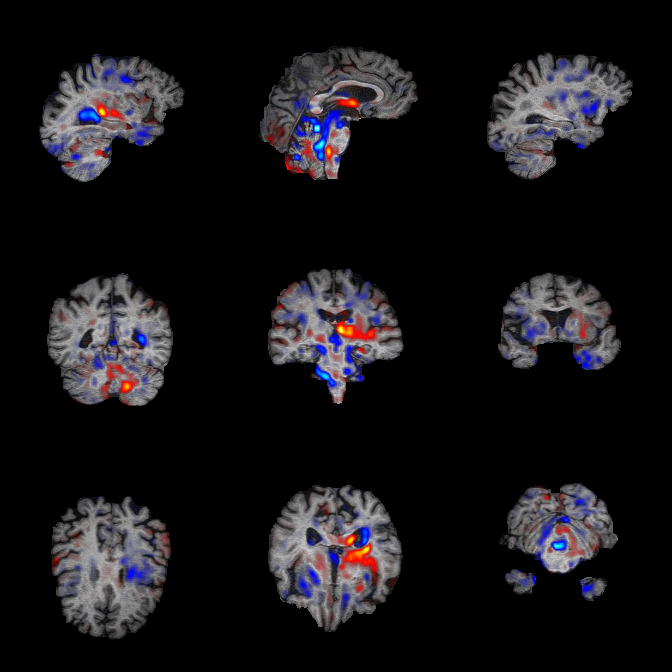
\includegraphics[width=4cm]{data/explanation_simple.png}
			};
			\node[] at ($ (heatmap.south) + (0, -0.3) $) {
				$\hat{\mathrm{age}}=79.6$
			};
		\end{tikzpicture}
		\vfill
	\end{frame}

	\begin{frame}{Paper 4: Explainable brain age}
		\vfill
		\centering
		\begin{tikzpicture}
			\node[outer sep=0pt, inner sep=0pt] (heatmap1) at (-3.5, -4) {
				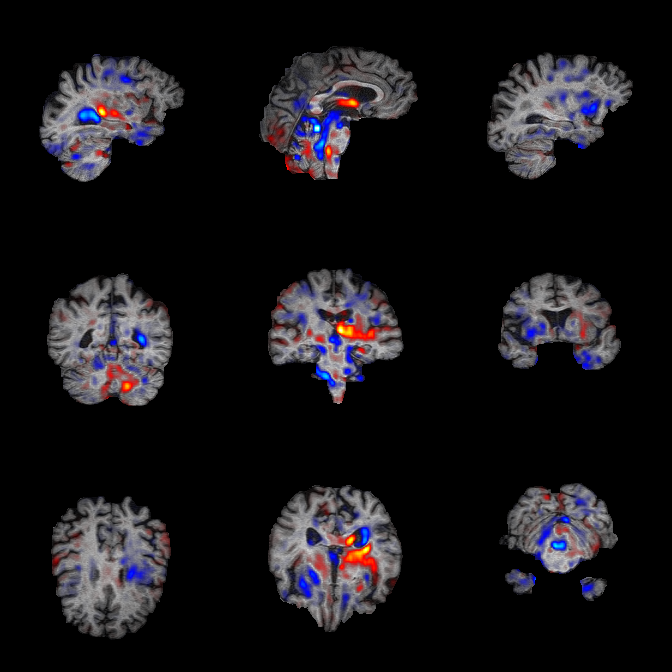
\includegraphics[width=3cm]{data/explanation_50.png}
			};
			\node[outer sep=0pt, inner sep=0pt] (heatmap2) at (0, -4) {
				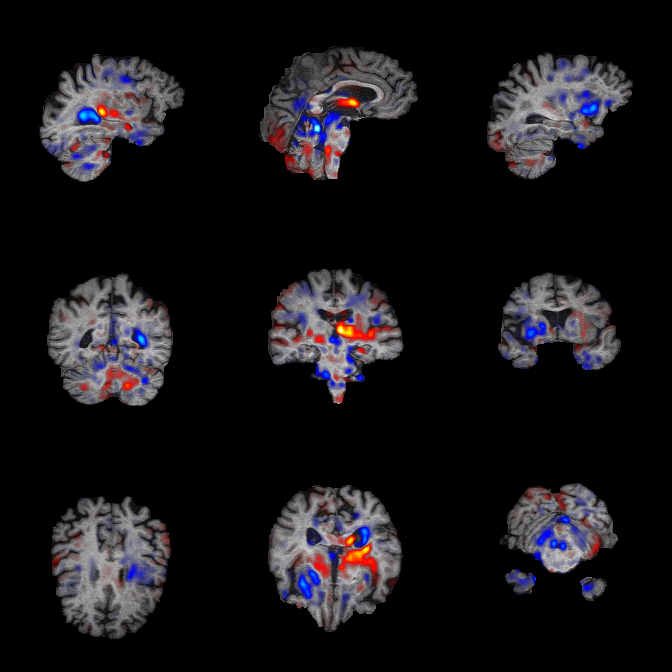
\includegraphics[width=3cm]{data/explanation_70.png}
			};
			\node[outer sep=0pt, inner sep=0pt] (heatmap3) at (3.5, -4) {
				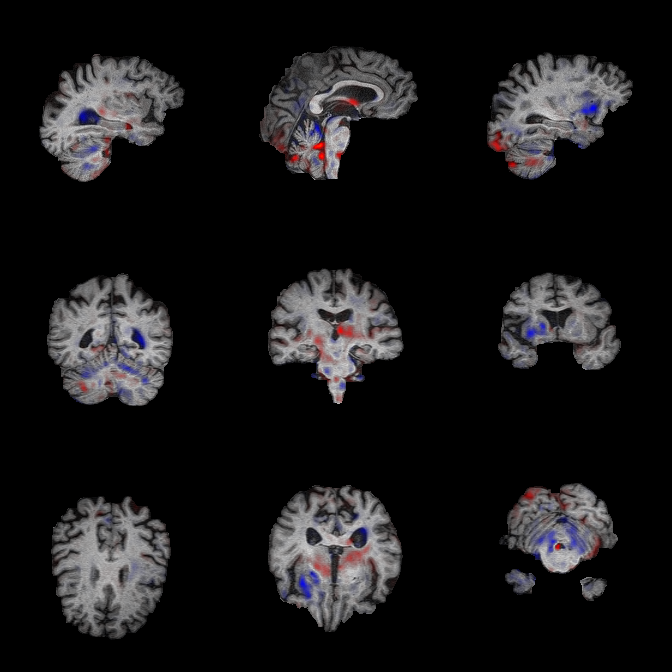
\includegraphics[width=3cm]{data/explanation_90.png}
			};
			\node[] at ($ (heatmap1.south) + (0, -0.3) $) {
				$\delta_{50}=29.6$
			};
			\node[] at ($ (heatmap2.south) + (0, -0.3) $) {
				$\delta_{70}=9.6$
			};
			\node[] at ($ (heatmap3.south) + (0, -0.3) $) {
				$\delta_{90}=-10.4$
			};
		\end{tikzpicture}
		\vfill
	\end{frame}

	\begin{frame}{Practical stuff}
		\begin{itemize}
			\item[\textcolor{green}{\checkmark}] 35/30 credits
			\item[\textcolor{green}{\checkmark}] Presented at conference
			\item[\textcolor{orange}{?}] ?/? teaching hours (PSY9511 this fall)
			\item[\textcolor{green}{\checkmark}] Public dissemination
			\item[\textcolor{green}{\checkmark}] Open source contributions
		\end{itemize}
	\end{frame}
\end{document}
